%\documentclass[12pt,twoside=semi,a4paper]{scrbook}
\documentclass[11pt,fleqn]{book}

%----------------------------------------------------------------------------------------
%	VARIOUS REQUIRED PACKAGES AND CONFIGURATIONS
%----------------------------------------------------------------------------------------

\usepackage[top=3cm,bottom=3cm,left=3cm,right=3cm,headsep=10pt,a4paper]{geometry} % Page margins
 
\usepackage{graphicx} 
\usepackage[english]{babel}
%\usepackage{enumitem} % Customize lists
% \setlist{nolistsep} % Reduce spacing between bullet points and numbered lists
% 
% \usepackage{booktabs} % Required for nicer horizontal rules in tables
% 
% \usepackage{marvosym}
% 
\usepackage{xcolor} % Required for specifying colors by name
\definecolor{grey}{rgb}{0.7,0.7,0.9} % Define the orange color used for
\definecolor{darkgrey}{rgb}{0.1,0.1,0.1} % Define the orange color used for
\definecolor{ocre}{RGB}{243,102,25} % Define the orange color used for highlighting throughout the book
% \definecolor{aureolin}{rgb}{0.99, 0.93, 0.0} % Define the yellow color used for
% 
% \definecolor{airforceblue}{rgb}{0.36, 0.54, 0.66}% Define the blue color used for
% 
% 


\parskip 1.5ex % paragraph spacing

 
% %----------------------------------------------------------------------------------------
% %	THEOREM STYLES
% %----------------------------------------------------------------------------------------
% 
% \usepackage{amsmath,amsfonts,amssymb,amsthm} % For math equations, theorems, symbols, etc
% 
% \newcommand{\intoo}[2]{\mathopen{]}#1\,;#2\mathclose{[}}
% \newcommand{\ud}{\mathop{\mathrm{{}d}}\mathopen{}}
% \newcommand{\intff}[2]{\mathopen{[}#1\,;#2\mathclose{]}}
% \newtheorem{notation}{Notation}[chapter]
% 
% % Boxed/framed environments
% \newtheoremstyle{ocrenumbox}% % Theorem style name
% {0pt}% Space above
% {0pt}% Space below
% {\normalfont}% % Body font
% {}% Indent amount
% {\small\bf\sffamily\color{ocre}}% % Theorem head font
% {\;}% Punctuation after theorem head
% {0.25em}% Space after theorem head
% {\small\sffamily\color{ocre}\thmname{#1}\nobreakspace\thmnumber{\@ifnotempty{#1}{}\@upn{#2}}% Theorem text (e.g. Theorem 2.1)
% \thmnote{\nobreakspace\the\thm@notefont\sffamily\bfseries\color{black}---\nobreakspace#3.}} % Optional theorem note
% \renewcommand{\qedsymbol}{$\blacksquare$}% Optional qed square
% 
% \newtheoremstyle{blacknumex}% Theorem style name
% {5pt}% Space above
% {5pt}% Space below
% {\normalfont}% Body font
% {} % Indent amount
% {\small\bf\sffamily}% Theorem head font
% {\;}% Punctuation after theorem head
% {0.25em}% Space after theorem head
% {\small\sffamily{\tiny\ensuremath{\blacksquare}}\nobreakspace\thmname{#1}\nobreakspace\thmnumber{\@ifnotempty{#1}{}\@upn{#2}}% Theorem text (e.g. Theorem 2.1)
% \thmnote{\nobreakspace\the\thm@notefont\sffamily\bfseries---\nobreakspace#3.}}% Optional theorem note
% 
% \newtheoremstyle{blacknumbox} % Theorem style name
% {0pt}% Space above
% {0pt}% Space below
% {\normalfont}% Body font
% {}% Indent amount
% {\small\bf\sffamily}% Theorem head font
% {\;}% Punctuation after theorem head
% {0.25em}% Space after theorem head
% {\small\sffamily\thmname{#1}\nobreakspace\thmnumber{\@ifnotempty{#1}{}\@upn{#2}}% Theorem text (e.g. Theorem 2.1)
% \thmnote{\nobreakspace\the\thm@notefont\sffamily\bfseries---\nobreakspace#3.}}% Optional theorem note
% 
% % Non-boxed/non-framed environments
% \newtheoremstyle{ocrenum}% % Theorem style name
% {5pt}% Space above
% {5pt}% Space below
% {\normalfont}% % Body font
% {}% Indent amount
% {\small\bf\sffamily\color{ocre}}% % Theorem head font
% {\;}% Punctuation after theorem head
% {0.25em}% Space after theorem head
% {\small\sffamily\color{ocre}\thmname{#1}\nobreakspace\thmnumber{\@ifnotempty{#1}{}\@upn{#2}}% Theorem text (e.g. Theorem 2.1)
% \thmnote{\nobreakspace\the\thm@notefont\sffamily\bfseries\color{black}---\nobreakspace#3.}} % Optional theorem note
% \renewcommand{\qedsymbol}{$\blacksquare$}% Optional qed square
% \makeatother
% 
% % Defines the theorem text style for each type of theorem to one of the three styles above
% \newcounter{dummy} 
% \numberwithin{dummy}{section}
% \theoremstyle{ocrenumbox}
% \newtheorem{theoremeT}[dummy]{Theorem}
% \newtheorem{problem}{Problem}[chapter]
% \newtheorem{exerciseT}{Exercise}[chapter]
% \newtheorem{designT}{Design philosophy}[chapter]
% \theoremstyle{blacknumbox}
% \newtheorem{infoT}{Note}[chapter] % icon: \Info
% \newtheorem{warningT}{Warning}[chapter] % icon: \danger
% \newtheorem{exampleT}{Example}[chapter]
% \theoremstyle{blacknumbox}
% \newtheorem{vocabulary}{Vocabulary}[chapter]
% \newtheorem{definitionT}{Definition}[section]
% \newtheorem{corollaryT}[dummy]{Corollary}
% \theoremstyle{ocrenum}
% \newtheorem{proposition}[dummy]{Proposition}
% 
% %----------------------------------------------------------------------------------------
% %	DEFINITION OF COLORED BOXES
% %----------------------------------------------------------------------------------------
% 
% \RequirePackage[framemethod=default]{mdframed} % Required for creating the theorem, definition, exercise and corollary boxes
% 
% % Theorem box
% \newmdenv[skipabove=7pt,
% skipbelow=7pt,
% backgroundcolor=black!5,
% linecolor=ocre,
% innerleftmargin=5pt,
% innerrightmargin=5pt,
% innertopmargin=5pt,
% leftmargin=0cm,
% rightmargin=0cm,
% innerbottommargin=5pt]{tBox}
% 
% % Exercise box	  
% \newmdenv[skipabove=7pt,
% skipbelow=7pt,
% rightline=false,
% leftline=true,
% topline=false,
% bottomline=false,
% backgroundcolor=ocre!10,
% linecolor=ocre,
% innerleftmargin=5pt,
% innerrightmargin=5pt,
% innertopmargin=5pt,
% innerbottommargin=5pt,
% leftmargin=0cm,
% rightmargin=0cm,
% linewidth=4pt]{eBox}	
% 
% % Definition box
% \newmdenv[skipabove=7pt,
% skipbelow=7pt,
% rightline=false,
% leftline=true,
% topline=false,
% bottomline=false,
% linecolor=ocre,
% innerleftmargin=5pt,
% innerrightmargin=5pt,
% innertopmargin=0pt,
% leftmargin=0cm,
% rightmargin=0cm,
% linewidth=4pt,
% innerbottommargin=0pt]{dBox}
% 
% % Corollary box
% \newmdenv[skipabove=7pt,
% skipbelow=7pt,
% rightline=false,
% leftline=true,
% topline=false,
% bottomline=false,
% linecolor=gray,
% backgroundcolor=black!5,
% innerleftmargin=5pt,
% innerrightmargin=5pt,
% innertopmargin=5pt,
% leftmargin=0cm,
% rightmargin=0cm,
% linewidth=4pt,
% innerbottommargin=5pt]{cBox}
% 
% % Corollary style
% \mdfdefinestyle{cBoxStyle}{%
% skipabove=7pt,
% skipbelow=7pt,
% rightline=false,
% leftline=true,
% topline=false,
% bottomline=false,
% linecolor=gray,
% backgroundcolor=black!5,
% innerleftmargin=5pt,
% innerrightmargin=5pt,
% innertopmargin=5pt,
% leftmargin=0cm,
% rightmargin=0cm,
% linewidth=4pt,
% innerbottommargin=5pt
% }
% 
% % Warning box
% \newmdenv[skipabove=7pt,
% skipbelow=7pt,
% rightline=false,
% leftline=true,
% topline=false,
% bottomline=false,
% linecolor=aureolin, 
% backgroundcolor=aureolin!20,
% innerleftmargin=5pt,
% innerrightmargin=5pt,
% innertopmargin=5pt,
% innerbottommargin=5pt,
% leftmargin=0cm,
% rightmargin=0cm,
% linewidth=4pt,
% innerbottommargin=0pt]{wBox}
% 
% % Info box
% \newmdenv[skipabove=7pt,
% skipbelow=7pt,
% rightline=false,
% leftline=true,
% topline=false,
% bottomline=false,
% linecolor=airforceblue, 
% backgroundcolor=airforceblue!20,
% innerleftmargin=5pt,
% innerrightmargin=5pt,
% innertopmargin=5pt,
% innerbottommargin=5pt,
% leftmargin=0cm,
% rightmargin=0cm,
% linewidth=4pt,
% innerbottommargin=0pt]{iBox}
% 
% % Creates an environment for each type of theorem and assigns it a theorem text style from the "Theorem Styles" section above and a colored box from above
% \newenvironment{theorem}{\begin{tBox}\begin{theoremeT}}{\end{theoremeT}\end{tBox}}
% \newenvironment{exercise}{\begin{eBox}\begin{exerciseT}}{\hfill{\color{ocre}\tiny\ensuremath{\blacksquare}}\end{exerciseT}\end{eBox}}	
% \newenvironment{design}{\begin{eBox}\begin{designT}}{\end{designT}\end{eBox}}
% \newenvironment{definition}{\begin{dBox}\begin{definitionT}}{\end{definitionT}\end{dBox}}	
% \newenvironment{example}{\begin{exampleT}}{\hfill{\tiny\ensuremath{\blacksquare}}\end{exampleT}}		
% \newenvironment{corollary}{\begin{cBox}\begin{corollaryT}}{\end{corollaryT}\end{cBox}}	
% \newenvironment{warning}{\begin{wBox}\begin{warningT}}{\end{warningT}\end{wBox}}
% \newenvironment{info}{\begin{iBox}\begin{infoT}}{\end{infoT}\end{iBox}}
% 
% %----------------------------------------------------------------------------------------
% %	REMARK ENVIRONMENT
% %----------------------------------------------------------------------------------------
\usepackage{tikz} 


\newenvironment{remark}{\par\vspace{10pt}\small % Vertical white space above the remark and smaller font size
 \begin{list}{}{
 \leftmargin=35pt % Indentation on the left
 \rightmargin=25pt}\item\ignorespaces % Indentation on the right
 \makebox[-2.5pt]{
\begin{tikzpicture}[overlay]
 \node[draw=ocre!60,line width=1pt,circle,fill=ocre!25,font=\sffamily\bfseries,inner sep=2pt,outer sep=0pt] at (-15pt,0pt){\textcolor{ocre}{R}};\end{tikzpicture}} % Orange R in a circle
 \advance\baselineskip -1pt}{\end{list}\vskip5pt} % Tighter line spacing and white space after remark


\newenvironment{definition}{\par\vspace{10pt}\small 
 \begin{list}{}{
 \leftmargin=35pt % Indentation on the left
 \rightmargin=25pt}\item\ignorespaces % Indentation on the right
 \makebox[-2.5pt]{
\begin{tikzpicture}[overlay]
 \node[draw=ocre!60,line
 width=1pt,circle,fill=ocre!25,font=\sffamily\bfseries,inner sep=2pt,outer sep=0pt] at (-15pt,0pt){\textcolor{ocre}{D}};\end{tikzpicture}} % Orange R in a circle
 \advance\baselineskip -1pt}{\end{list}\vskip5pt} % Tighter line spacing and white space after remark
 
% %----------------------------------------------------------------------------------------
% %	SECTION NUMBERING IN THE MARGIN
% %----------------------------------------------------------------------------------------
% 
% \makeatletter
% \renewcommand{\@seccntformat}[1]{\llap{\textcolor{ocre}{\csname the#1\endcsname}\hspace{1em}}}                    
% \renewcommand{\section}{\@startsection{section}{1}{\z@}
% {-4ex \@plus -1ex \@minus -.4ex}
% {1ex \@plus.2ex }
% {\normalfont\large\sffamily\bfseries}}
% \renewcommand{\subsection}{\@startsection {subsection}{2}{\z@}
% {-3ex \@plus -0.1ex \@minus -.4ex}
% {0.5ex \@plus.2ex }
% {\normalfont\sffamily\bfseries}}
% \renewcommand{\subsubsection}{\@startsection {subsubsection}{3}{\z@}
% {-2ex \@plus -0.1ex \@minus -.2ex}
% {.2ex \@plus.2ex }
% {\normalfont\small\sffamily\bfseries}}                        
% \renewcommand\paragraph{\@startsection{paragraph}{4}{\z@}
% {-2ex \@plus-.2ex \@minus .2ex}
% {.1ex}
% {\normalfont\small\sffamily\bfseries}}
% 
 
\usepackage{hyperref}
\hypersetup{hidelinks,backref=true,pagebackref=true,hyperindex=true,colorlinks=false,breaklinks=true,urlcolor= ocre,bookmarks=true,bookmarksopen=false,pdftitle={Title},pdfauthor={Author}}

\hypersetup{
  pdftitle={Peano Cookbook},
  pdfauthor={Tobias Weinzierl},
  pdfsubject={Peano Cookbook}
}



\usepackage{listings}


\lstdefinelanguage{cCCode}[]{C}{
   backgroundcolor=\color{grey},
 %  basicstyle=\tiny,
 %  basicstyle=\small,
   basicstyle=\footnotesize,
   stringstyle=\color{red},
   keywordstyle=\color{blue},
   commentstyle=\color{darkgrey}\slshape,
   morekeywords={linestyle,linetype,linewidth,linecolor,pointtype,nohidden3d,hidden3d,palette,lt,lw,lc,pt,ps,fd,fill,fs,ls},
   framexleftmargin=1mm, framextopmargin=1mm, frame=shadowbox,
   rulesepcolor=\color{darkgrey}
 }
 
 
 
     
\lstnewenvironment{code}[1][]{
\lstset{
 language=cCCode,#1,
upquote=true,
columns=fullflexible,
literate={*}{{\char42}}1
         {-}{{\char45}}1
}}{}
     
     


% \usepackage{geometry}
% \usepackage{amsmath, amssymb, amsthm}
% \usepackage{graphicx}
% \usepackage{color}
% \usepackage{framed}
% \usepackage{listings} 
% \usepackage{hyperref}
% \usepackage[utf8]{inputenc}
% \usepackage{tgpagella}
% 
% 
% \geometry{left=3.5cm,textwidth=15cm,top=3cm,textheight=23cm}



\begin{document}

 
\begin{titlepage}

{ \large
  \begin{center}

  TECHNISCHE UNIVERSIT\"AT M\"UNCHEN \\
%  Technische Universit\"at M\"unchen\\
  \vspace{.3cm} 
  Department of Informatics \\
  Scientific Computing

  \vspace{4cm}
   Habilitationsverfahren Dr.~rer.~nat.~Tobias Weinzierl
  
  \vspace{1.5cm}

{\Huge
Cumulative Habilitation
}
\\
\vspace{1cm}
and 
\\
\vspace{0.6cm}
{\Huge
Progress Report\\
}

%   Dr.~rer.~nat.~Tobias Weinzierl
  \vspace{1.5cm}

%  \today
  \end{center}
}


\end{titlepage}


 \thispagestyle{empty}
 \newpage
 \cleardoublepage 

 \pagestyle{plain}
 \pagenumbering{roman}
 \chapter{Preamble}


\Peano\ is an open source framework for solvers on dynamically adaptive
Cartesian meshes.
Its core is built with C++, but many tools around it are written in Python.
\Peano\  is based upon the fact that spacetrees, a generalisation of the classical octree concept, yield a cascade of adaptive Cartesian grids. Consequently, any spacetree traversal is equivalent to an element-wise traversal of the hierarchy of the adaptive Cartesian grids. The software \Peano\  realises such a grid traversal and storage algorithm, and it provides hook-in points for applications performing per-element, per-vertex, and so forth operations on the grid. It also provides interfaces for dynamic load balancing, sophisticated geometry representations, and other features. Some properties are enlisted below.

Peano is currently available in its fourth generation. 
The development of the original set of Peano codes started around 2002.
2005-2009, we merged these codes into one Peano kernel (2nd generation). 
In 2009, I started a complete reimplementation of the kernel with special
emphasis on reusability, application-independent design and the support for rapid prototyping. 
This third generation of the code ended around 2019 when we released the
ExaHyPE code---a hyperbolic equation system solver engine which uses Peano's
AMR meshes.
The current guidebook discusses \Peano\ , which reuses ideas and lessons learned
from Peano~3 as well as lots of code buildling blocks, but can be seen as a
major rewrite starting from scratch.



\Peano\ has been the code base for multiple projects over the past years.
The most prominent one is likely ExaHyPE.
The first generation of ExaHyPE has been a stand-alone projects using Peano
as one required library or framework out of many.
The second generation, \ExaHyPE, is merged into \Peano as spin-off.
This document therefore covers \ExaHyPE, too.




\section*{Dependencies and prerequisites}

\Peano's core is plain C++17 code. 
We however use a whole set of tools around it:

\begin{itemize}
  \item GNU autotools (automake) to set up the system (required).
  \item C++17-compatible C++ compiler (required).
  \item Python3 (optional; not required if you work only with the C++
  baseline).
  \item MPI2 (optional). MPI's multithreaded support is required.
  \item Intel's Threading Building Blocks or OpenMP 5. We also can work with C++
  threads, but found their performance suboptimal.
  \item The Visualization Toolkit (VTK) if you want to use the built-in
  visualisation facilities (optional).
  \item Doxygen if you want to create HTML pages of PDFs of the in-code
  documentation.
\end{itemize}

\begin{remark}
I test and maintain \Peano\  for Linux only.
If you prefer Windows or MacOS, it should work as long as you provide the
mandatory tools from above, but I won't be able to help.
\end{remark}


\begin{center}
 \begin{tabular}{|l|l|p{8cm}|}
  \hline
   Software & Version & Remarks \\
  \hline
   GNU g++ & 7.5 or older & Works with \Peano\ core but not with some extensions
   such as \ExaHyPE. \\
   GNU g++ & 9.3.1 & Current development version. Works. \\
  \hline
   Intel icpc & 19.1 & Works with \Peano\ and all
   extensions such as \ExaHyPE. Tests with Intel Fortran have been successful,
   too. \\
  \hline
   VTK & 7--9 & Supported by \Peano. Default is 8, i.e.~if you need other
   version, you have to inform configure (see Chapter \ref{chapter:postprocessing}). \\
   \hline
   Python & 3 & Development version. Python 2 is not supported by frontend. \\
   \hline
 \end{tabular}
\end{center}

\section*{Who should read this document}

This cookbook is written similar to a tutorial in a hands-on style.
Therefore, it also contains lots of source code snippets.
If you read through a chapter, you should immediately be able to re-program the
presented details in your code and use the ideas.

Therefore, this cookbook is written for people that have a decent programming
background as well as scientific computing knowledge.
% Some background in the particular application area's algorithms for some
% chapters also is required. 
It is a cookbook that shall help readers to translate their scientific vision
into a working code quickly.


\section*{How the text is organised}

% This book covers a variety of problems I have tackled with Peano when I wrote
% scientific papers.
% There is no overall read thread through the document.
% I recommend to start reading some chapters and then jump into chapters
% that are of particular interest.
% Whenever something comes to my mind that should be added, I will add it.
If you feel something is urgently missing and deserves a chapter or things
remain unclear, please write me an email and I'll see whether I can provide some
additional text or extend the cookbook.


{
  \flushright
  \today 
  \\ 
  Tobias Weinzierl 
  \\
}

 

 \cleardoublepage 
 
 \tableofcontents

 \newpage

 \cleardoublepage 

 \pagestyle{plain}
 \pagenumbering{arabic}
 
 \chapter{Installation}

There are two ways to obtain \Peano: 
You can either download one of the archives we provide on the webpage, or you
can work directly against a repository clone (recommended).
If you work with the archive, type in a 
\begin{code}
tar -xzvf myarchive.tar.gz
\end{code}
in the directory where you've stored your downloaded file.


If you work with the git archive, you have to clone this archive first. 
I grant access to \Peano\  free of charge and the repository is public.
However, I ask users to sign up for the software if they indend to push
modifications to the code (which I very much appreciate\footnote{\Peano's
guidebook (the file you currently read) is hosted within \Peano's git
repository, too. I'm always happy if people add content to this
documentation, too.}).
This way I can report to funding agencies how frequent the software is used, and
I also have at least some ideas which application areas benefit from the
software and where it is actively used and developed.
If you do not indend to modify the \Peano\ core code base, you can just clone
the code anomymously.

\begin{code}
git clone https://gitlab.lrz.de/hpcsoftware/Peano.git
cd Peano
git checkout p4
\end{code}


\begin{remark}
I still maintain the ``old'' Peano in the repository (version 3), and most users
consider this to be the standard Peano generation.
For the present document, it is thus important that you manually switch to the
branch \texttt{p4}.
\end{remark}



\section{Prepare the configure environment}

This step should only required if you work directly against the git repository.
If you prefer to download a snapshot of \Peano, then you can skip this section
and continue with \ref{section:installation:configure}.


\begin{itemize}
  \item Ensure you have the autotool packages installed on your system. They
  typically are shipped in the packages \texttt{autoconf}, \texttt{automake} and
  \texttt{libtool}.
  \item Set up the configure environment: 
 \begin{code}
 libtoolize; aclocal; autoconf; autoheader; 
 cp src/config.h.in .; 
 automake --add-missing
 \end{code}
\end{itemize}


\noindent
These steps should only be required once, unless you push major revisions to the
development branch.


\section{Configure}
\label{section:installation:configure}


\Peano\  relies on the autotools to set up its build environment.
Change into the project's directory and type in 
\begin{code}
./configure --help
\end{code}


\noindent
The \texttt{--help} option should give you some information about the available
variants of \Peano.
A sole \texttt{./configure} call gives you the minimalist version of
\Peano---might be appropriate for a first test.

\begin{remark}
 I recommend that you start a first test without any additional flavours of
 \Peano, i.e.~to work with a plain \texttt{./configure} call. Once the tests
 pass, I recommend that you add further options (IO) and/or parallelisation.
 Please note that the baseline config is not sufficient for most applications
 as it is merely a stripped down version of the \Peano\ core.
 \ExaHyPE\ for example requires you to add \texttt{--enable-exahype} and
 \texttt{--enable-loadbalancing-toolbox}. 
 But the bare/minimal version is good for first tests.
\end{remark}


\noindent
The output of \texttt{./configure --help} should be reasonable verbose, but I
summarise some key options below:

\begin{center}
 \begin{longtable}{lp{10cm}}
  \texttt{--with-multithreading} & Switch on multithreading. By default, we
  build without multithreading, but a \texttt{--with-multithreading=omp}, e.g.,
  makes \Peano\  use the OpenMP threading model. Please consult \texttt{--help} for
  details. Note: To use OpenMP multithreading, you will need a compiler which
  supports OpenMP 5.0 (e.g - GCC 9.x)\footnote{\Peano\ realises its GPGPU
  offloading via OpenMP, too. Some compilers struggle to translate these GPGPU
  instructions. In this case, please configure with the CXXFLAG
  \texttt{-DnoGPUOffloading}.}.
   \\
  \texttt{--with-mpi} & Enable the MPI version of \Peano. You have to tell the
  build environment however which compile command to use. Please note that
  we need a C++ MPI wrapper. So \texttt{--with-mpi=mpcxx} is a typical call. Currently, you also need \texttt{--with-multithreading} if you want to use MPI. 
   \\
  \texttt{--with-vtk} & Inform \Peano\  that VTK is available on the system.
  \Peano\ mainly
  relies on its own IO data format. Even some VTK dump routines (used usually
  only for debugging) are written by hand, i.e.~do not rely on the VTK
  libraries.
  However, \Peano\ comes along with some command line conversion tools that can convert its tailored data
  dumps into VTK, and they do rely on the VTK libraries. With this flag, you
  tell \Peano\ to build these tools.
  The VTK installation is sometimes not easy (and you might have to provide additional parameters depending on your installation). I dedicate Chapter \ref{chapter:postprocessing} on VTK.
   \\
  \texttt{--with-hdf5} & Make \Peano\  support HDF5 output. Not stable at the
  moment.
   \\
  \texttt{--with-delta} & Configure \Peano\  such that the geometry library
  $\Delta $ is used. Not stable at the moment.
   \\
  \texttt{--with-toolchain} & Build against a particular vendor toolchain.
  Currently, I have dedicated support for the NVIDIA NVTX SDK
  (\texttt{--with-toolchain=nvidia}) providing NVIDIA-specific logging/tracing
  as well as memory allocation calls---the latter is of use if you use
  GPUs---and the Intel toolchain (\texttt{--with-toolchain=intel}). The latter
  in particular links against the ITAC tracing API. I also have support for
  Google's Chrome browser (\texttt{--with-toolchain=chrome}) which means that
  traces are written in a way that you can display it in Chrome. Ensure that your CXXFLAGS set the right include path\footnote{It is
  \texttt{CXXFLAGS+=-I/opt/nvidia/nsight-systems/2020.3.1/target-linux-x64/nvtx/include/nvtx3/}
  on my system, e.g.}.
  This is optional.
   \\
  \texttt{--with-gpu} & Add GPGPU support. Depending on the target, we currently
  have specialised versions for NVIDIA (\texttt{--with-gpu=nvidia}) and AMD
  (\texttt{--with-gpu=amd}). For different vendors, you might be required to
  select particular multithreading models. The AMD and NVIDIA port for example
  work only with OpenMP.
   \\
  \texttt{--enable-exahype} & Includes the \ExaHyPE\ core into your build.
   Requires the load balancing toolbox, too. 
   \\
  \texttt{--enable-xxx-toolbox} & \Peano\ is shipped with a couple of toolboxes
   for various purposes. These are C++ libraries which offer a lot of features.
   You have to enable/activate them manually. Please note: Not all toolboxes are
   compatible with all targets. We have experienced issues with the
   FEM toolbox and some GPGPU systems for example.
 \end{longtable}
\end{center}




\noindent
Compilers, linkers and both compiler and linker flags can be changed by
resetting the corresponding environment variables (such as
\texttt{CXX} or \texttt{LDFLAGS} or \texttt{CCFLAGS}) \emph{prior} to the
configure call.
Alternatively, you can pass the variables to be used to \texttt{configure}
	through arguments (\texttt{./configure CXX=icpc ...}, e.g.). 
Please consult the \texttt{--help} output for details.
For some supercomputers that we use frequently, there are recommendations which
setting to use (Chapter~\ref{chapter:selected-HPC-platforms}).


\begin{remark}
Most Linux tools prefer you to specify a dedicated installation directory via
\texttt{--prefix}.
For \Peano, things are slightly different: \Peano\ is a mere engine, i.e.~not
``useful'' per se.
It is applications built on top of \Peano\ that become tools that you might
later want to install/deploy on your system. 
Therefore, I ship \Peano\ with static libraries only, and most users work with
the code in the download/installation directory until they have constructed the
application with the help of \Peano.
So no need to specify a proper installation directory via \texttt{--prefix}.
\end{remark}


%   \texttt{--prefix=/mypath} & Will install \Peano\  in \texttt{/mypath}.
%    \\


\section{Build}

Once the configuration has been successful, a simple 
\begin{code}
make
\end{code}
should build the \Peano\ core.
It also builds some examples and all the extensions and toolboxes you have
manually enabled.
All of these go into static libraries.
The code is not small and you thus might prefer
\begin{code}
make -jx
\end{code}
with x being the number of parallel builds to use.


\begin{remark}
 Following up on the remark above, 
 \begin{code}
make install
 \end{code}
 would deploy the \Peano\ files in the directory specified via the
 \texttt{prefix} before.
 Most Unix tools want you to install them. 
 For \Peano, things might be slightly different as it is an engine used to
 construct tools in the first place. 
\end{remark}





\section{Installation test}

Once you have compiled \Peano\, I recommend that you run all tests using

\begin{code}
  make check
\end{code}

\noindent
The call launches all of \Peano's unit test, i.e.~all the unit tests for the
core plus the extensions that you have enabled.


\begin{remark}
 I have written the test target such that it works out-of-the-box for non-MPI
 calls. If you have configured with \texttt{--with-mpi}, then the unit tests
 will fail. But this does not mean that the unit tests are broken. It is simply
 due to the fact that the makefile's test target does not know that you have to
 use the \texttt{mpirun} prefix.
 To make a long story short: If you use MPI and you want to run the unit tests,
 you have to do so manually.
\end{remark}


\noindent
To run 2D and 3D tests individually, use

\begin{code}
  src/unittests/UnitTests2d
  src/unittests/UnitTests3d
\end{code}

\noindent
You can run these builds with different core counts and also MPI support if you
have compiled with MPI.
The executables contain both node correctness tests and MPI ping-pong tests,
i.e.~you can both assess a valid build plus a working MPI environment.
If successful, you should always get a message alike

\begin{code}
Peano 4 (C) www.peano-framework.org 
build: 2d, with mpi (1 ranks), omp (4 threads), debug level=4
it is recommended that you run the unit tests with more than one MPI rank, too (file:main.cpp,line:82)
usage: ././UnitTests2d core-count (use default core count=1 now) (file:main.cpp,line:88)
running test case collection "tarch.la.tests" ..... ok
running test case collection "tarch.la" ............. ok
running test case collection "tarch.mpi.tests" ..... ok
running test case collection "tarch.mpi" ... ok
running test case collection "tarch" ... ok
running test case collection ... ok
running test case collection "peano4.grid.tests" ....... ok
running test case collection "peano4.grid" ... ok
running test case collection "peano4.parallel.tests" ....... ok
running test case collection "peano4.parallel" ... ok
running test case collection "peano4" ... ok
running test case collection ... ok
\end{code}

\noindent
Watch out for the last line that tells you whether the overall unit tests passed
through.

\section{Python configuration}

\Peano\ is developed with Python 3. Python 2 is not supported. 


\subsection{Python paths}
To make any Python example pass, you have to set the Python paths.
There are multiple ways to do so.

The standard way is to set the \texttt{PYTHONPATH}:
\begin{code}
export PYTHONPATH=myPeanoDirectory/python
\end{code}
This can even be done in the \texttt{.bashrc}.

Alternatively, you can augment your Python scripts later on with 
\begin{code}
import sys
PEANO4_PYTHON_DIR="myPeanoDirectory/python"
sys.path.append(PEANO4_PYTHON_DIR)
\end{code}


\noindent
Please note that most Python scripts require you to set the
\texttt{LD\_LIBRARY\_PATH}. 
If you install \Peano, then this path should be automatically right.
If you work with a local \Peano\ installation, you can either tell \Peano\
through its API where to search for the library (all routines that add a
library accept additional search paths), or you can again use the
\texttt{sys.path.append} command to extend \texttt{LD\_LIBRARY\_PATH}.


\begin{remark}
 I personally prefer the variant to go through the environment variable.
 \Peano's Python API yield plain old makefiles building executables that work
 completely without any Python. 
 This way, we ensure that we work smoothly on supercomputers, too, where Python
 sometimes is not available in the latest version or on the compute nodes.
 As long as you run through environment variables or the \Peano\ routines to
 specify paths, your makefiles also will continue to work that way. 
\end{remark}


\subsection{Python packages}

\Peano\ currently relies on the following Python packages/projects:


\begin{center}
 \begin{tabular}{lp{6cm}ll}\\
   Package & Description & Ubuntu & OpenSUSE \\
   \hline
   jinja2 & For all the templated glue code. & 
    \texttt{python3-jinja2} &
    \texttt{} 
    \\
   sympy & For the symbolic modelling of partial differential equations
    (predominantly in \ExaHyPE). &
    \texttt{python3-sympy} &
    \texttt{python3-sympy} 
 \end{tabular}
\end{center}


\noindent
The table above specifies the corresponding packages in our two main
distributions for which we test \Peano. 
They can be installed via \texttt{zypper install} (SUSE) or \texttt{apt-get
install} (Ubuntu), respectively.
Alternatively, you might want to use Python's \texttt{pip}.





\section{Fortran}

\begin{remark} 
 If you don't use Fortran in your own code, ignore this section.
\end{remark}

\Peano's core does not use any Fortran at all. 
However, many users use Fortran for their domain-specific programming.
If you want to have a seemless integration of your particular Fortran choice
through \Peano's Python API, invoke \texttt{./configure} ensuring that the
Fortran variables---in particular the environment variable \texttt{FC}
identifying the compiler---are properly set.


For many codes and the GNU Fortran compiler, you need the flag
\texttt{-fdefault-real-8}.
You can export \texttt{FCFLAGS} and make it contain this argument before you
invoke \texttt{configure}.
As the \Peano's core does not use Fortran---it is only applications built on top
of \Peano---you can redefine the flags later on (see \ref{section:installation:applications-built-with-Peano}).



\section{\Peano\ components and build variants}
\label{chapter:installation:build-variants}

\Peano\ currently is delivered as a set of archives, i.e.~static libraries:
\begin{itemize}
  \item There is a technical architecture (\texttt{Tarch}) and the actual
  \texttt{Peano4Core}.
  \item Each archive variant is available as a release version, as a debug
  version, as a version with tracing and assertions and as a tracing-only
  version.
  \item Each archive variant is available as 2d build and as 3d build. If you
  need higher dimensions, you have to build the required libraries manually.
\end{itemize}


The version terminology is as follows:
\begin{itemize}
  \item {\bf debug} The debug versions of the archives all have the postfix
  \texttt{\_debug}. If you link against these versions, the full set of
  assertions, of all tracing and all debug messages is available; though you can
  always filter on the application-level which information you want to see
  (cmp.~Chapter \ref{section:logging}).
  \item {\bf asserts} Thsee versions of the archives all have the postfix
  \texttt{\_asserts}. If you link against these versions, all assertions are on.
  The code also contains tracing macros (see below).
  \item {\bf tracing} The release versions of the archives all have the postfix
  \texttt{\_trace}. If you link against these versions, all assertions and debug
  messages are removed, but some tracing is active. You can switch on/off the
  tracing per class (cmp.~Chapter \ref{section:logging}), and different tracing
  backends allow you to connect to different (profiling) tools.
  \item {\bf release} The release versions of the archives have no
  particular postfix. They disable tracing, any debugging and all assertions.
  These archives should be used by production runs.
\end{itemize}


\begin{remark}
 Peano's release components still write info messages (they suppress debug,
 tracing and logging, but not essential information). If you want to filter out
 these messages, too, you have to apply a log filter (Chapter
 \ref{section:logging:log-filter}).
\end{remark}


\noindent
Besides these archives, the \Peano\ installation also comes along with a set of
example applications.
They are found in the directory \texttt{src/examples}.
Most examples create by default two variants of the example: a debug
version and one with only tracing enabled.
Several examples furthermore come along as 2d and 3d build.



\section{Documentation}

\begin{figure}
 \begin{center}
  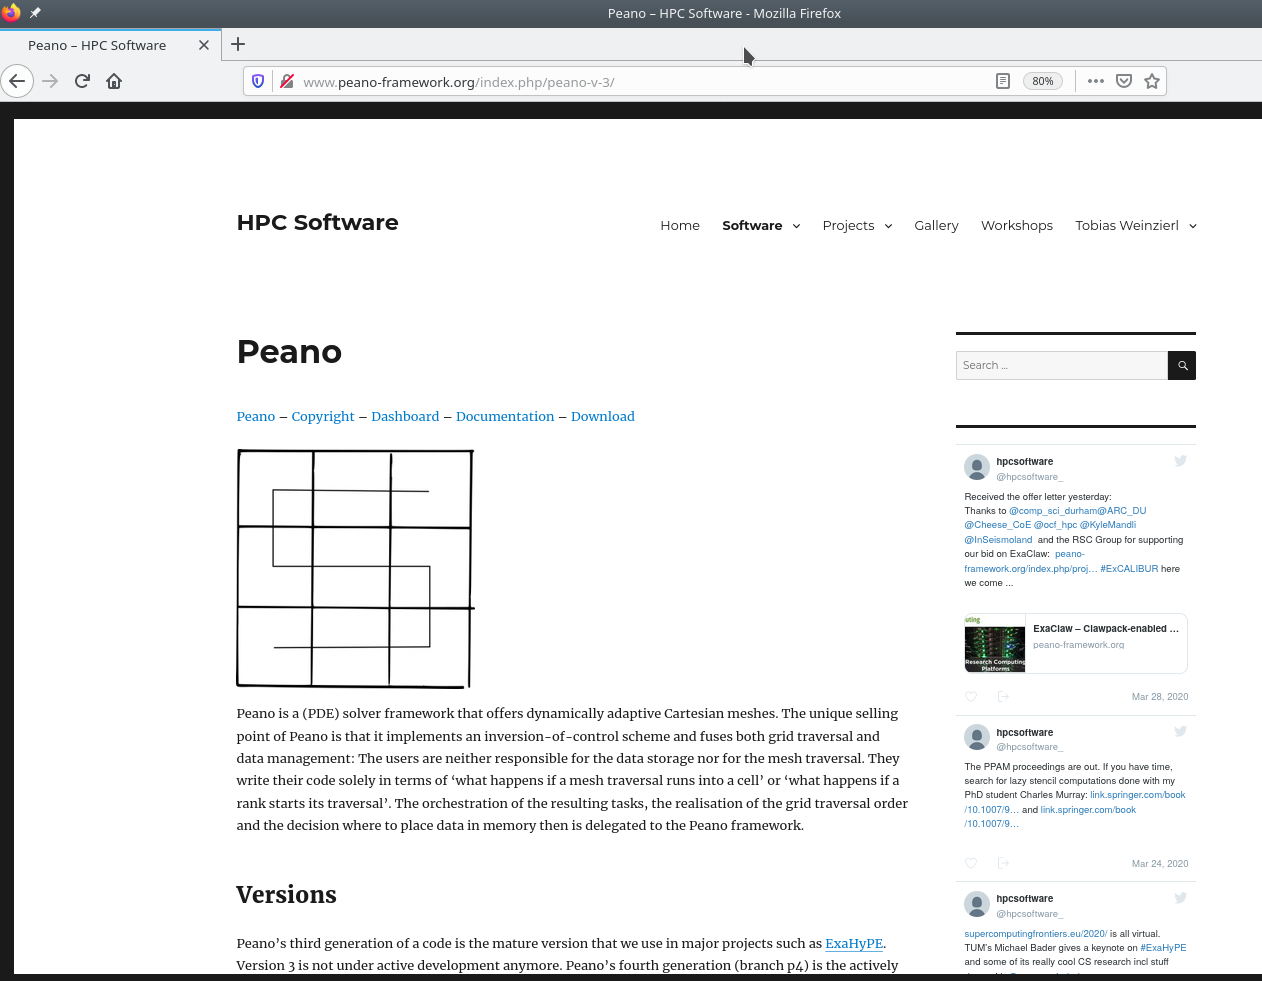
\includegraphics[width=0.4\textwidth]{10_installation/webpage.png}
  \hspace{0.4cm}
  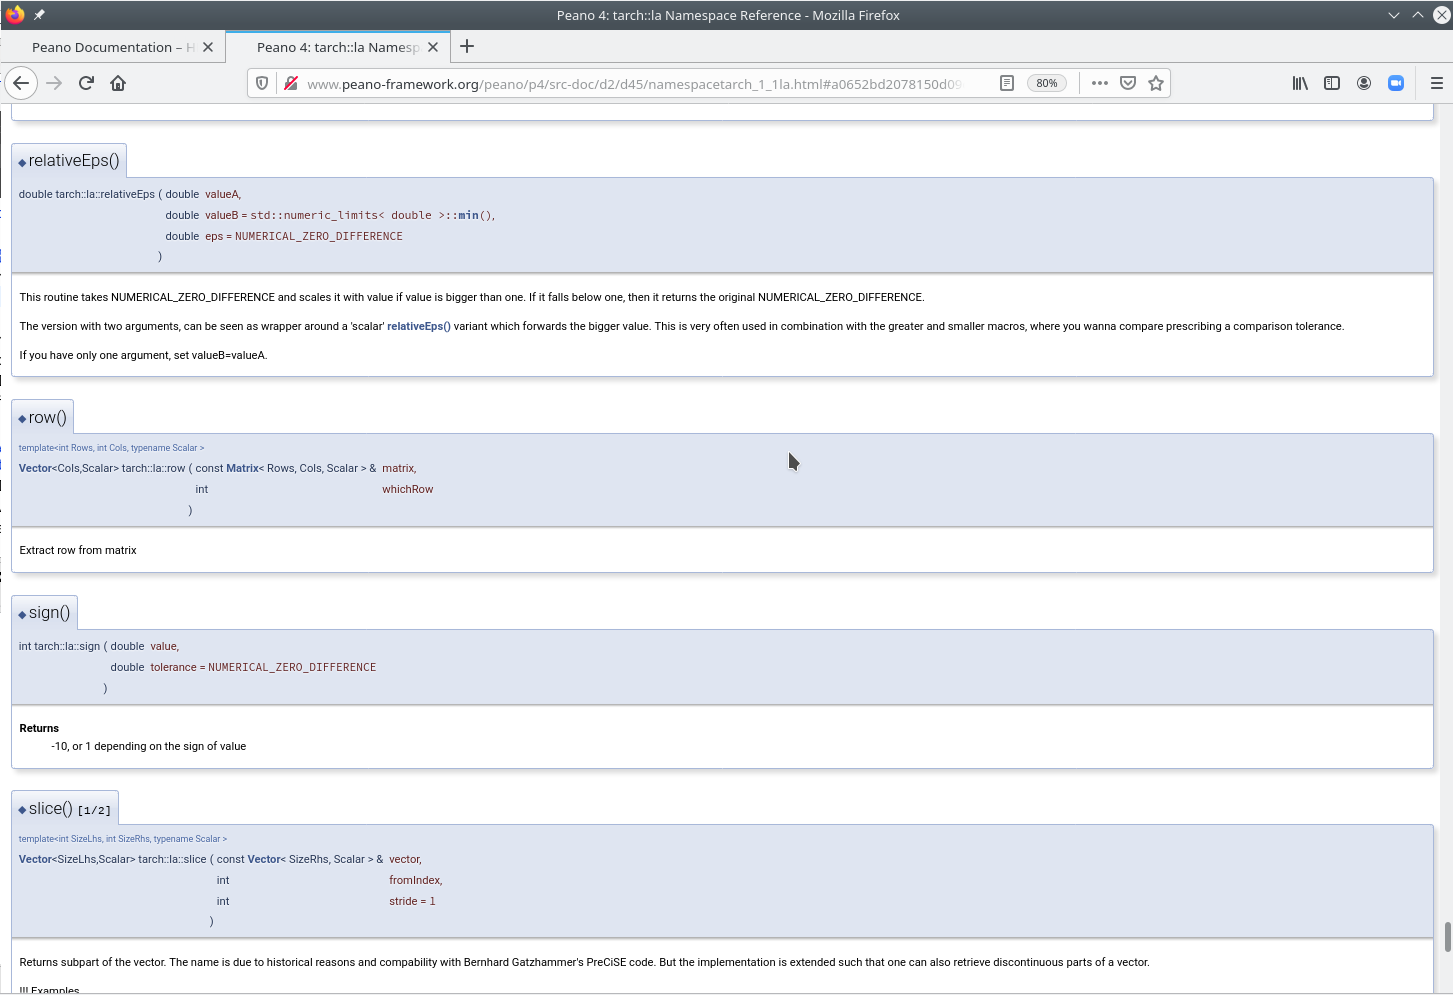
\includegraphics[width=0.4\textwidth]{10_installation/source-docu.png}
 \end{center}
 \caption{
  \Peano's webpage (left) and a screenshot from the auto-generated source code
  docu which can be reached through the webpage if you don't want to generate
  the pages yourself.
  This documentation also provides indices and a search function as well as all
  documentation formulae typeset with LaTeX.
 }
\end{figure}



There are three major types/resources of documentation of the software:
\begin{enumerate}
  \item This guidebook/cookbook that describes how to use the code base from a
  high abstraction level and with anecdotal examples.
  \item The documentation of the C++ code. Here, I follow an ``everything is in
  the code'' philosophy.
  \item The documentation of the Python code. Here, I follow an ``everything is
  in the code'' philosophy.
\end{enumerate}

\noindent
For the code documentation, ``everything is in the code'' means that all
documentation is comments within the Python script or C++ header files,
respectively.
You can create a webpage from this distributed information through
the tool \texttt{doxygen}\footnote{\url{http://www.doxygen.nl}.}. 


There are two Doxygen configuration files in the repository, i.e.~I keep the
Python and the C++ documentation output separate.
To create the documentation, switch into directory \texttt{src} or
\texttt{python}, respectively. 
In both directories, the Doxygen config file is called
\texttt{peano.doxygen-configuration}, i.e.~calling

\begin{code}
doxygen peano.doxygen-configuration
\end{code}

\noindent
gives you the output. If you prefer not to generate and maintain the
documentation yourself, the \Peano\ webpage hosts the autogenerated
documentation, too.
It is updated roughly once a week.



\section{Compile/link options for applications built with \Peano}
\label{section:installation:applications-built-with-Peano}

\Peano\ is a framework, i.e.~ships very few executables (mainly only for test
purposes and for postprocessing).
Its core delivery is a set of libraries.
Application codes then build on top of these libraries.
While it is up to you to decide which build system you use in your application,
\Peano\ natively favours makefiles.


If you use \Peano's Python API, it will create dummy makefiles.
Higher-level \Peano\ applicaitons such as \ExaHyPE\ build upon the Python API
and thus work with makefiles, too.
When they create these makefiles, they parse your local \Peano\ installation's
makefiles and extract the information from there.
This is, when you've selected a particular compiler or compiler option when you
install \Peano, this choice will automatically propagate through to your
domain-specific codes.
There's however the option to overwrite the chosen settings---either by defining
appropriate environment variables before you invoke \texttt{make} or by
resetting variables manually within your Python scripts that configure the
environment.




 \chapter{\Peano's architecture}
\label{chapter:architecture}




 \part{Large-scale \Peano\ applications}
 \newpage
 \chapter{\ExaHyPE}
\label{section:exahype}


\begin{figure}[htb]
 \begin{center}
  
\includegraphics[width=0.2\textwidth]{60_exahype/EU.png}
  
\includegraphics[width=0.5\textwidth]{60_exahype/ExaHyPE_Logo.jpg}
 \end{center}
 \caption{
   The original ExaHyPE project delivering the first generation of the ExaHyPE
   software has received funding from the European Union’s Horizon 2020 research
   and innovation programme under grant agreement No 671698 (ExaHyPE).
 }
\end{figure}

\noindent
\ExaHyPE\ is the follow-up development of the ExaHyPE project which has been
funded by the EU from 2015--2019.
The present version is the second generation of the code (\ExaHyPE) and has
seen substantial rewrites of core routines.
However, many paradigms and even code blocks remain the same.
Migrating from the original ExaHyPE to \ExaHyPE\ thus should be straightforward.


\ExaHyPE\ is both a set of C/C++ and Fortran core routines complementing the
\Peano\ core and a high-level augmentation of \Peano's Python API.
Compare to the architecture sketch from Chapter \ref{chapter:architecture}.
\ExaHyPE's Python API can be read as builder mechanism:
You configure your particular \ExaHyPE\ application, i.e.~you tell the \ExaHyPE\
engine which application you want to run (which PDE terms, which solver
variants, which hardware properties).
The Python API then yields both a \Peano\ Python project which you can run plus
a set of template classes which you implement with your particular application.


The present document discusses how to create an \ExaHyPE\ application from
scratch.
Most application experts might not want to do this and instead use a read-to-use
\ExaHyPE\ application.
The most prominent (and maybe powerful) code using the ExaHyPE engine is maybe
ExaSeis; used to simulate seismic waves.
The details of these domain-specific codes are not covered by the present
document.



\section*{Preparing \Peano\ to run \ExaHyPE}

It is relatively straightforward to use \ExaHyPE\ within \Peano:

\begin{itemize}
  \item Configure your code with the flag \texttt{--enable-exahype}.
  \item Recompile your code. This should give you a couple of
  \texttt{ExaHyPE2Core} libraries in the respective subdirectories.
  \item Ensure that \texttt{python/exahype} is in your Python search path.
\end{itemize}


\section*{Difference of \ExaHyPE\ vs.~ExaHyPE (first generation)}

The original ExaHyPE had been built on top of Peano (third generation) and tried
to hide as much of Peano away as possible.
In \ExaHyPE, I go the opposite way: \ExaHyPE\ is a full-blown Peano add-in and I
try not to hide anything away.
Where we designed our own data management on top of Peano in ExaHyPE, all the
data management (as well as parallelisation, e.g.) is native \Peano.


With the migration from a sole-C++ philosophy to C++ supplemented by a Python
API in \Peano, I also dumped ExaHyPE's former configuration/specification file
pradigma.
An \ExaHyPE\ application now is championed by a sole Python script.
This Python script yields a native \Peano\ application (builder mechanism) which
then assembles the application.



\section{Minimalistic Finite Volumes for the Euler equations}
\label{section:exahype:fv}

We provide a complete Finite Volume implementation of a plain Euler solver
realised with \ExaHyPE. 
This solver relies on a Rusanov flux and can, with only a few lines, be
changed into an ADER-DG scheme later.
Indeed, it can be used by an ADER-DG scheme as a limiter later on.
All example data can be found within the directory
\texttt{python/examples/exahype2/finitevolumes}.


\subsection{Preparation}

Our centrel Euler script first includes a couple of tools that we need to work
with \ExaHyPE:

\begin{code}
import peano4
import peano4.datamodel
import peano4.solversteps
import peano4.output
import peano4.visualisation
import peano4.toolbox.blockstructured

import exahype2
\end{code} 


\noindent
Different to a \Peano\ application, we now do create an \ExaHyPE\ project
instance
\begin{code}
project = exahype2.Project( ["examples", "exahype2", "finitevolumes"], "finitevolumes", "." )
\end{code}
\noindent
which is assigned a subnamespace, a project name and an output path.


Next, we add the Finite Volumes solver to the project. 
This step also specifies the number of unknowns and the patch sizes that we want
to use:
\begin{code}
patch_size = 25
unknowns   = 5
project.add_finite_volumes_solver("Euler", patch_size, unknowns, 0.0001)
\end{code}
\noindent
The solver is called \texttt{Euler}.


Once this minimalist \ExaHyPE\ project is done, we ask it to generate a \Peano\
project for us, let this project parse our configure script's outcome (so that
we use the same compiler settings and other options), and we also tell \Peano\
where to find our \ExaHyPE\ libraries.
Please note that \Peano\ builds these libraries in different variants
(production runs, tracing or debugging flavours, \ldots).
Select the right one:

\begin{code}
peano4_project = project.generate_Peano4_project()
peano4_project.output.makefile.parse_configure_script_outcome( "../../../.." )
peano4_project.output.makefile.add_library( "ExaHyPE2Core2d_debug", "../../../../src/exahype2" )
peano4_project.generate(peano4.output.Overwrite.Default)
peano4_project.build()
\end{code}


\noindent
To run this code---won't work as we lack the actual Physics in the
implementations---type in
\begin{code}
success = peano4_project.run( [] )
\end{code}
within the Python workbench. 
Alternatively, you can build/run the code directly from the command line. 

\begin{definition}
 \Peano\ and, hence, \ExaHyPE\ provide the Python API to model the application. 
 Under the hood, they rely on a plain makefile and generate a stand-alone C++
 application without Python-dependencies.
 So once you've created your application, nothing stops you from dropping the
 Python front-end. 
 Once you've built you application, you don't need Python anymore (within your
 Slurm script, e.g.).
\end{definition}



\subsection{Implementing the Euler solver}

The run of \ExaHyPE\ so far has given us a lot of glue code (which we will
never touch) and three files in the main directory:
\texttt{AbstractEuler.h}, \texttt{Euler.h} and \texttt{Euler.cpp}.

\begin{definition}
  In \ExaHyPE's native mode, i.e.~without further packages such as Ghoddess or
  ClawPack, I always create two classes per solver: an abstract superclass and
  the actual implementation class.
  The latter has to implement all routines from the abstract superclass which
  are not yet defined.
  For some of the routines, I provide empty glue code with a todo remark. 
  For most of them, just open the (abstract) header file, browse through the
  code and create implementations in the subclass manually.
\end{definition}

\noindent
It is the last one that we have to alter to inject our domain knowledge,
i.e.~the PDE\footnote{If you regenerate your \ExaHyPE\ code later on, it will
overwrite the Abstract\ldots solver classes, but it will never modify your
actual solver instances. So if signatures change, your implementation won't
get lost.}.
In our introductory example, there are three routines that require our
attention.
The first one is \texttt{adjustSolution}.
We can use this routine to overwrite the solution at any time and, hence, to
inject boundary conditions or stimuli into the domain.
It is also this routine that allows us to realise initial conditions:
\begin{code}
void examples::exahype2::finitevolumes::Euler::adjustSolution(
  double Q[5],
  const tarch::la::Vector<Dimensions,double>&  x,
  const tarch::la::Vector<Dimensions,double>&  h,
  const tarch::la::Vector<Dimensions,double>&  t
) {
  if (tarch::la::equals(t,0.0) ) {
    // initial conditions
    bool isInTheCentre = ( tarch::la::norm2( x-tarch::la::Vector<Dimensions,double>(0.5) ) < 0.05 );
    Q[0] = 1.0;  // rho
    Q[1] = 0;    // velocities
    Q[2] = 0;
    Q[3] = 0;
    Q[4] = isInTheCentre ? 1.0 : 0.0; // inner energy
  }
}
\end{code}


\noindent
As second and third step, we have to write our actual flux and eigenvalue
functions as we need them for Rusanov:

\attachfile[icon=Paperclip,description=Download code snippet,author=Peano 4]
{60_exahype/Euler-eigenvalues.cpp}

\begin{code}
void examples::exahype2::finitevolumes::Euler::eigenvalues(
  double                                       Q[5],
  const tarch::la::Vector<Dimensions,double>&  faceCentre,
  const tarch::la::Vector<Dimensions,double>&  volumeH,
  const tarch::la::Vector<Dimensions,double>&  t,
  int                                          normal,
  double                                       lambda[5]
) {
  [...]
}
\end{code}



\attachfile[icon=Paperclip,description=Download code snippet,author=Peano 4]
{60_exahype/Euler-flux.cpp}


\begin{code}
void examples::exahype2::finitevolumes::Euler::flux(
  double                                       Q[5],
  const tarch::la::Vector<Dimensions,double>&  faceCentre,
  const tarch::la::Vector<Dimensions,double>&  volumeH,
  const tarch::la::Vector<Dimensions,double>&  t,
  int                                          normal,
  double                                       F[5]
) {
  [...]
}
\end{code}


\noindent
There are quite a lot of assertions in the code in the repository that you might
want to skip (and I didn't paste them in here).
I found them useful when I wrote \ExaHyPE\ in the first place.
With these implementations in place, you can finally type in \texttt{make} in
the project directory and rerun the code.
Alternatively, just re-execute the whole Python script.
You'll get your first wave equation solver

Some simple boundary conditions close the system:

\begin{code}
void examples::exahype2::finitevolumes::Euler::boundaryConditions(
  double                                       Qinside[5],
  double                                       Qoutside[5],
  const tarch::la::Vector<Dimensions,double>&  faceCentre,
  const tarch::la::Vector<Dimensions,double>&  volumeH,
  const tarch::la::Vector<Dimensions,double>&  t,
  int                                          normal
) {
  Qoutside[0] = Qinside[0];
  Qoutside[1] = Qinside[1];
  Qoutside[2] = Qinside[2];
  Qoutside[3] = Qinside[3];
  Qoutside[4] = Qinside[4];
}
\end{code}



\subsection{Configuring the overall run}

\ExaHyPE's Python interface gives you the opportunity to specify exactly which
domain you want to use, how often to plot, and when to shut down the simulation.
For a first trial, we set the parameters as follows:
\begin{code}
project.set_global_simulation_parameters(
  2,         # Dimensions
  [0.0,0.0], # Offset of computational domain
  [1.0,1.0], # Size of computational domain
  0.2,       # Terminal time, i.e. we simulate from 0 to 0.2
  0.0,       # First snapshot of solution is done after grid construction, i.e. at time 0
  0.001      # We then plot every 0.001 time units
)
\end{code}
\noindent
This is all. We now can run the code.


\subsubsection{IO and logging}


\ExaHyPE\ codes by default yield snapshots in \Peano's block format. 
If you have configured \Peano\ with VTK support, you can directly convert it
into VTK and visualise through Paraview or VisIt, e.g.:
\begin{code}
if success:
  convert = peano4.visualisation.Convert( "solutionEuler" )
  convert.set_visualisation_tools_path( "../../../../src/visualisation" )
  convert.extract_fine_grid()
  convert.convert_to_vtk()
\end{code}


\ExaHyPE\ searches for a text file \texttt{exahype.log-filter} in the working
directory.
If no such file is found (or the file is corrupted), then it will use some
default filter rules, i.e.~dump the information to the terminal that I consider
to be most important.
If you want to adopt the output, I strongly recommend that you add a log filter
configuration file. 
The syntax of log filter files is discussed in Section
\ref{section:logging:log-filter}.



\subsection{Running on a parallel computer}

To run \ExaHyPE\ in parallel, you have to build \Peano\ with support for
multithreading and/or MPI.
Once this is done, the engine more or less runs in parallel out of the box.


\paragraph{Domain decomposition}
The core domain decomposition scheme realised in \ExaHyPE\ is a non-overlapping
multiscale domain decomposition based upon space-filling curves (SFC).
To use this scheme, you have to specify an appropriate load balancing scheme.
Without any load balancing, the code will never split up the domain and thus
effectively run serially.

\begin{figure}
 \begin{center}
  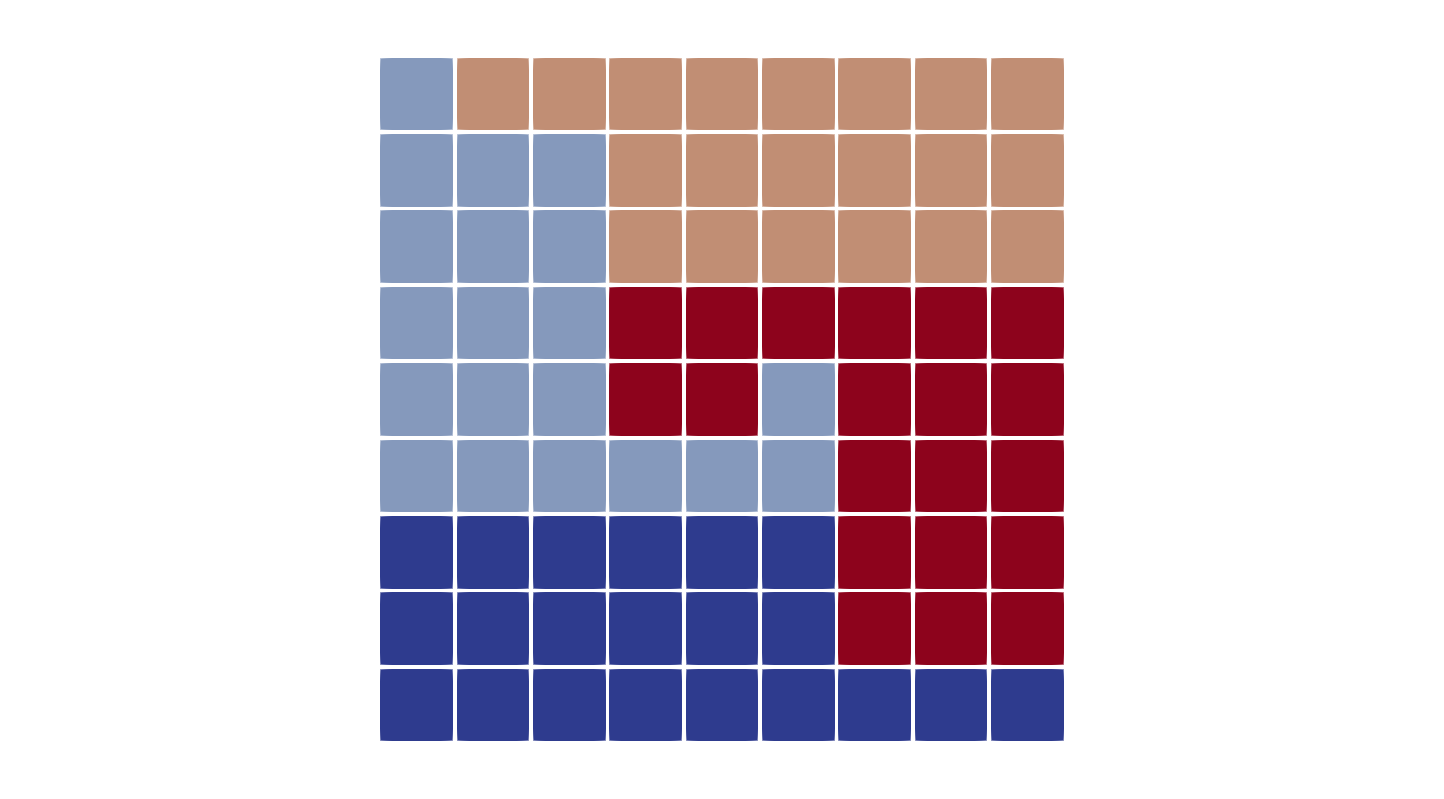
\includegraphics[width=0.54\textwidth]{60_exahype/domain-decomposition.png}
 \end{center}
 \caption{
  Domain decomposition in \ExaHyPE\ for a run with four threads/ranks. Each
  individual cell hosts a patch.
 }
\end{figure}


I plan to support multiple different dynamic load balancing schemes over time,
but the straightforward decomposition scheme shipped with \Peano\ at the moment
is recursive subdivision, a modification of OpenMP's guided scheduling.
To use it, you have to call
\begin{code}
project.set_load_balancing( "toolbox::loadbalancing::RecursiveSubdivision" )
\end{code}

\noindent
on your \ExaHyPE\ project. You can add  


\paragraph{Task decomposition}
\ExaHyPE\ realises an additional task decomposition working on top of the domain
decomposition. 
This task decomposition is shared memory, only.
That is, you can use task decomposition without domain decomposition, but then
you won't benefit from multiple nodes.
You can however always use domain decomposition without task
decomposition---though it should be slower in most cases.

\begin{remark}
This section is under construction.
\end{remark} 


\section{GPU support}

To add GPU support (via OpenMP 5), you have to do a couple of steps.
First, your environment has to be compiled with OpenMP, and I strongly recommend
that you also add \texttt{--with-nvidia} to have support for their tools.
Check that \texttt{-DnoGPUOffloading} is \emph{not} set within the compile
flags and translate your code.

Next, ensure that you use an \ExaHyPE\ solver which has support for GPUs. 
The enclave solvers typically are your solvers of choice.
Solvers that provide GPU support have a flag \texttt{use\_gpu} in their
constructor which is unset by default. 
Set it to \texttt{True} and rerun the toolkit.

\begin{definition}{Solvers with GPU support}
 A solver can use GPUs if and only if can provide all of its PDE terms
 including the eigenvalue computations (so the functions \texttt{flux},
 \texttt{eigenvalues}, \texttt{nonconservativeProducts}, \ldots) as stateless
 functions without side-effects, i.e.~functions that can be written down as
 static and do not need (or even alter) any attribute of the solver class.
\end{definition}

\noindent
If you solver does not fit to this class, it is not a fit for GPUs.
If it fits, then please create two versions of the eigenvalue function and all
of the PDE term functions (such as the flux computations) in your solver.
Keep the original one, and add a second one which is 

\begin{itemize}
  \item static and 
  \item accepts an additional flag of type \texttt{
  tarch::multicore::TargetDevice}.
\end{itemize}

\noindent
You will need to include 
\begin{code}
#include "tarch/multicore/multicore.h"
\end{code} 

\noindent
explicitly. Very often, the standard flux and eigenvalue routines can invoke the
static variants and you can thus eliminate redundancies.
Please note that solvers with GPU support still can have states in their PDE
terms, i.e.~alter solver variables.
But they can do so only for cells which we call skeletons (see the paper by
Charrier et al.~on enclave tasking).


Finally, add
\begin{code}
#if defined(GPUOffloading)
#pragma omp declare target
#endif

my new static function variants

#if defined(GPUOffloading)
#pragma omp end declare target
#endif
\end{code} 






\section{Modelling the fluxes and Riemann solvers with SymPy}

You can model your fluxes, Riemann solvers and so forth with SymPy, 
i.e.~through symbolic formulations.
For this, you have to install the computer algebra system on your
system.
The computer algebra extension to specify solver ingredients is held within the
\ExaHyPE\ subpackage \texttt{exahype2.sympy}.


I provide a couple of classes to model PDEs in different formulations and are
held within the subpackage \texttt{peano4.solvers.sympy}.
They wrap around SymPy's symbolic expressions, and thus allow users to work with
these expressions directly.
On top of that they offer some code generation which again wraps SymPy's code
generation plus then adds all the glue to integrate this code generation into a
\Peano\ solver.


The Euler equations modelled via this interface then add the following code
snippet to the Python script that models \Peano:

\begin{code}
import sympy
import exahype2.solvers.sympy.FirstOrderConservativePDEFormulation


#
# Create a new instance of symbolic ExaHyPE PDE interface.
#
pde = exahype2.solvers.sympy.FirstOrderConservativePDEFormulation(unknowns = 5,dimensions = 3)

#
# Give entries in input vector symbolic names. We first declare some
# helpers/constants. Then we tell the solver how we would like to name the Q 
# entries
#
gamma = sympy.symbols( "gamma")
rho   = pde.name_Q_entry( 0, "rho" )
j     = pde.name_Q_entries( 1, 3, "j" )
E     = pde.name_Q_entry( 4, "E" )

#
# Finally, define the equation system
#
p = (gamma - 1 ) * (E-1/2 * exahype2.solvers.sympy.dot(j,j) / rho)

pde.F[0,:]   = j
pde.F[1:4,:] = 1/rho * exahype2.solvers.sympy.outer(j,j) + p * sympy.eye(3)
pde.F[4,:]   = 1/rho * j * (E+p)

c = sympy.sqrt( gamma * p /rho )
pde.eigenvalue[0] = [ j[0]/rho - c, j[1]/rho - c, j[2]/rho - c ]
pde.eigenvalue[1] = [ j[0]/rho, j[1]/rho, j[2]/rho ]
pde.eigenvalue[2] = [ j[0]/rho, j[1]/rho, j[2]/rho ]
pde.eigenvalue[3] = [ j[0]/rho, j[1]/rho, j[2]/rho ]
pde.eigenvalue[4] = [ j[0]/rho + c, j[1]/rho + c, j[2]/rho + c ]

pde.substitute_expression( gamma, 1.4 )
\end{code}


\noindent
A simple
\begin{code}
 print( pde )
\end{code}
demonstrates what we have modelled.
This \texttt{pde} object here can create C++ code that we can plug directly into
the respective \Peano\ routines.


Key for economic modelling now however is the usage of the FV solver's
\texttt{set\_implementation} routine:
\begin{code}
my_solver.set_implementation( \
  flux=pde.implementation_of_flux(),eigenvalues=pde.implementation_of_eigenvalues())
\end{code}

\noindent
With this call, the modelled PDE goes, via code generation, directly into the
\ExaHyPE\ solver. When we remodel the PDE, everything is updated automatically.


If you study the interface of \texttt{set\_implementation}, you will notice that
you can also model boundary or initial conditions this way.
In this example, we however only modelled flux and eigenvalues.
The remaining callbacks remain plain C++.


For further resources, please visit SymPy's homepage, and maybe you also want to
have a look into projects like EinsteinPy or galgebra which provide tools for
astrophysics or geometric algebra, respectively.
As we rely on SymPy and expose all the SymPy expressions, they are compatible
with \ExaHyPE.




\section{Finite Volumes with ClawPack (ExaClaw)}

ExaClaw is an extension of \ExaHyPE\ (Chapter \ref{chapter:exahype}) which
offers the ClawPack Riemann solvers within \ExaHyPE.
Its development has been made possible by EPSRC under the Excalibur
Phase I call.
The grant number is EP/V00154X/1.


\begin{remark}
 This solver family is work-in-progress.
\end{remark}



\section{Ghoddess DG solvers}
% 
% We also do provide an interface to Ghoddess DG solvers.
% Ghoddess solvers use a classic DG formulation with explicit time stepping.
% Their big USP within \ExaHyPE\ is they rely on a quasi-symbolic formulation and
% thus facilitate even fast prototyping.
% 
\begin{remark}
  This yet has to be written.
\end{remark}
 
% \subsection{Preparation}
% 
% We first install Ghoddess:
% 
% \begin{remark}
%  Add instructions here.
% \end{remark}
% 
% 
% \subsection{Using the Ghoddess solver}
% 
% From hereon, our description follows the Finite Volume example from Section
% \ref{section:exahype:fv}, i.e.~we only highlight where we do things differently.
% Besides our \ExaHyPE\ modules, we first include the ghoddess subpackage which is
% not by default included:
% 
% \begin{code}
% import os
% import peano4
% import exahype2
% import exahype2.ghoddess
% \end{code} 
% 
% From hereon, we create the Ghoddess solver and add it to the project:
% 
% \begin{code}
% project = exahype2.Project( ["examples", "exahype2", "advection"], "ghoddess", "." )
% order          = 23
% unknowns       = 5
% time_step_size = 0.0001
% project.add_solver(  exahype2.ghoddess.RusanovLegendreWithFixedTimeStepSize(
%   "Advection", order, unknowns, 0.0001) )
% \end{code}



\section{Introducing a new numerical scheme}

This section discusses how to introduce a totally new numerical solver. 
It does not discuss how to introduce a new PDE, as new PDEs are built on top of
\ExaHyPE.
This section gives you an idea how to extend \ExaHyPE\ instead.

\begin{remark}
  \ExaHyPE\ is a very high level Python API which generates a \Peano\
   Python project which in turn creates the ``real'' \Peano\ C/C++ code. If you
   introduce a new numerical scheme/solver to \ExaHyPE, you thus might want to
   familiarise yourself with \Peano's Python API and how to extend it. This
   recommendation affects all the gluecode/framework aspects of the software.
   All the core numerics of \ExaHyPE\ are held as C++ code in the
   \texttt{src/exahype2} directly and compiled into a separate library. If you
   introduce new numerical schemes, you might have to extend this library, too.
\end{remark}



\subsection{A new Finite Volume solver (native \ExaHyPE)}

Introducing a new Finite Volume scheme is reasonably straightforward within
\ExaHyPE.
It relies directly on \Peano's patch-based AMR.


\begin{itemize}
  \item Create a new subclass of \texttt{exahype2.solver.FV}. The parent class
  has to be told with which patch overlaps you work.
  \item Instantiate this class in your user code when you invoke
  \texttt{add\_solver} on the \ExaHyPE\ project.
  \item Overwrite \texttt{get\_user\_includes()} to add all the includes for
  C/C++ code that you'll eventually need. 
  \item If you class is called \texttt{XYZ}, create four text files:
  \texttt{XYZAbstract.template.h}, \linebreak \texttt{XYZAbstract.template.cpp},
  \texttt{XYZ.template.h} and \texttt{XYZ.template.cpp}.
\end{itemize}

\noindent
\ExaHyPE's design concept is that each solver yields two types of classes:
The actual solver and an abstract superclasses. 
Abstract superclasses are regenerated every time you rerun the Python script.
Furthermore, they define the whole signature, i.e.~if you alter the signature
later on, users simply rerun the toolkit. 
Finally, the abstract superclasses hold default implementations.


With \Peano, you can create arbitrary abstract superclasses. 
They have to implement some general \ExaHyPE\ routines, but the number of operations that they have to
provide is very small.
I thought about introducing a general \texttt{exahype2::Solver} class, but then
this class is not really required anywhere as we work with code generation all
the way through anyway. 
So the only thing your solver's abstract superclass has to give \ExaHyPE\ is the
following set of routines:

\begin{code}
  double getMinTimeStamp() const;
  double getMaxTimeStamp() const;
  double getMinTimeStepSize() const;
  double getMaxTimeStepSize() const;

  void startTimeStep(
      double globalMinTimeStamp,
      double globalMaxTimeStamp,
      double globalMinTimeStepSize,
      double globalMaxTimeStepSize
  );

  void finishTimeStep();
\end{code}
\noindent
You can make them virtual if you want to highlight that a user can reimplement
them. 
But there's no need for this. 


The core implementation effort clearly has to go into the parts where the actual
mesh traversal is mapped onto solver calls.
In \ExaHyPE, this is realised through templates. 
Any user solver is supposed to define three local variables within its solver
class:
\texttt{HandleBoundaryTemplate}, 
\texttt{CreateCellTemplate}, \texttt{HandleCellTemplate} and
\texttt{AMRTemplate}.
There are more, but this is the minimum.


Within these templates, you have access to a couple of variables, some symbols,
and you can furthermore specify your own replacement rules:
\begin{itemize}
  \item Within each code block, you have access to a variable marker which is of
  type \texttt{peano4::datamanagement::FaceMarker} or
  \texttt{peano4::datamanagement::CellMarker}. It allows you to find out more
  about the face or cell centre, mesh sizes, \ldots, i.e.~it holds all spatial
  information.
  \item Within each code block, the constant \texttt{\{SOLVER\_INSTANCE\}} will
  be replaced by the Python code with an actual instance of your user's solver.
  \item The constant
  \texttt{\{NUMBER\_OF\_VOLUMES\_PER\_AXIS\}} will be replaced by the block size
  specified by the user. It is the attribute you hand through in the
  constructor.
  \item The constant
  \texttt{\{NUMBER\_OF\_UNKNOWNS\}} will be replaced by the argument you pass to
  the constructor.
  \item There are more constants. See \linebreak
  \texttt{peano4.solvers.FV.\_\_init\_dictionary\_with\_default\_parameters} for
  information.
  \item You can introduce more symbolds as \texttt{\{XYZ\}} as long as you add
  them within your routine
  \texttt{add\_entries\_to\_text\_replacement\_dictionary}.
\end{itemize}


\noindent
The template mechanism works similar to aspect-oriented programming, i.e.~it
simply enables Python to plug some code snippets straight into your the
generated \ExaHyPE\ code. 
The interesting thing however is the symbol

\begin{itemize}
  \item \texttt{fineGridCell\{UNKNOWN\_IDENTIFIER\}.value} which is a double
    pointer which points to the whole patch hosted by the cell in the volumetric
    routines \texttt{CreateCellTemplate}, \texttt{HandleCellTemplate} and
    \texttt{AMRTemplate}. The array it points to has the size \linebreak
    \texttt{\{NUMBER\_OF\_VOLUMES\_PER\_AXIS\}}$^d \cdot $
    \texttt{\{NUMBER\_OF\_UNKNOWNS\}}.
  \item \texttt{fineGridFace\{UNKNOWN\_IDENTIFIER\}.value} is the face
    equivalent for the boundary conditions. Again, it is a double pointer,
    though one dimension is not equal to
    \texttt{\{NUMBER\_OF\_VOLUMES\_PER\_AXIS\}} but equal to the halo overlap.
    See the Finite Volumes discussion in
    Chapter~\ref{section:python-api-examples:finite-volumes}.
  \item \texttt{reconstructedPatch} and \texttt{originalPatch} are only defined
    within \texttt{HandleCellTemplate}. The former is an alias for
    \texttt{fineGridFace\{UNKNOWN\_IDENTIFIER\}.value}, i.e.~points to the same
    location. \texttt{reconstructedPatch} is another pointer which points to the
    patch from the previous mesh traversal, i.e.~you can overwrite data
    within \texttt{originalPatch} and still have the old one available.
    Furthermore, the underlying patch is bigger: It hosts the actual patch data
    plus its halo.
\end{itemize}




\begin{remark}
 If you want to see a really simple example of this solver type, change into the 
 directory \texttt{src/exahype2/fv} and have a look into \texttt{Rusanov.cpp}.
 It follows exactly the above recipe.
\end{remark}


\noindent
I see two different ways how to realise a new solver: 
You can either code your solver directly within the Python templates.
Alternatively, you can generate some generic glue code within the template and
forward calls to some predefined C++ or user code.


Both variants have pros and cons and are valid.
For my generic Rusanov solver (as well as for ADER-DG), we can realise all
numerics generically within predefined kernels relying only on few user-defined
functions injecting flux and eigenvalues.
Furthermore, these functions have the same signature for all applications.
For a bespoke Finite Volume scheme where the Riemann solver holds the actual
numerical wisdom and each Riemann solvers requires a bespoke signature, it is
maybe better to skip that additional level of abstraction.



\subsection{Ghoddess implementation remarks}

Ghoddess works on triangles which we embed into the squares or cubes,
respectively, of \ExaHyPE.
By default, the code employs Gauss-Legendre sample points.
The data structure used thus read as follows
(Fig.~\ref{figure:60_exahype:degree-of-freedom-layout:Ghoddess}):
\begin{itemize}
  \item The solver embeds a ``patch'' of $N$ polynomial weights into each cell.
  For order $p=1, d=2$, we have for example $N=6$, for $p=2, d=2$ we have
  $N=12$.
  \item Each face carries $2(p+1)^{d-1}$ doubles.
\end{itemize}


\noindent
The face data holds a left and a right representation of the polynomial along
the face.
So it does not really hold degrees of freedom.
Its degree of freedom are mere projections of the cell solution onto the face.



\begin{figure}
 \begin{center}
  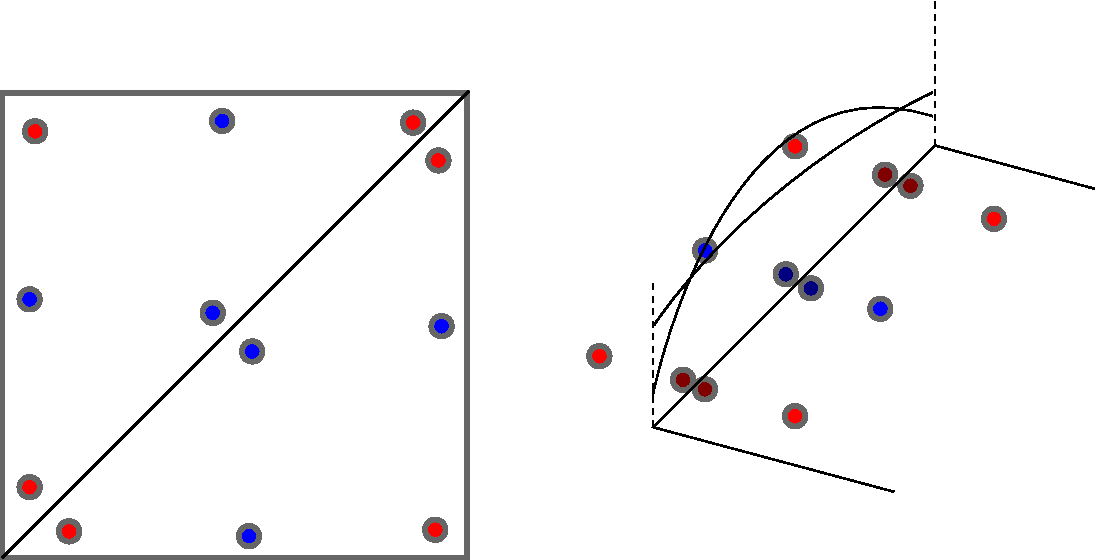
\includegraphics[width=0.65\textwidth]{60_exahype/Ghoddess-dof-layout.pdf}
 \end{center}
 \caption{
  Left: Degree of freedom layout in Ghoddess within a cell.
  Right: Each face holds additional ``degree of freedoms'' which encode the
  projection of the cell polynomial onto the face.
  \label{figure:60_exahype:degree-of-freedom-layout:Ghoddess}
 }
\end{figure}

The Ghoddess solver itself splits up into four computation kernels:

\begin{enumerate}
  \item The {\bf projectOntoFace} kernel accepts the $N$ degrees of freedom from
  the cell and projects the polynomials of the two triangles within the cell
  onto the faces. It consequently writes $2d \cdot (p+1)^{d-1}$ face DoFs. Once
  we have traversed the whole mesh, each face ``knows'' its left and right
  projection.
  \item The {\bf solveRiemann} kernel takes the $2 \cdot (p+1)^{d-1}$ DoFs on
  the face, i.e.~the left and right projection, and solves the Riemann problem
  on the jump. The result is written back into the $2 \cdot (p+1)^{d-1}$ DoFs.
  In principle, this allows us to have a different outgoing flux for the left
  and right side of a face.
  \item The {\bf solveCell} kernel evolves the solution within the triangle
  pair, i.e.~it evaluates the volumetric integrals of the DG formulation. The
  name is slightly wrong: Besides the volumetric terms, the kernel also
  evaluates the face terms arising between the two triangles embedded into the
  cell. So it is a combination of a cell kernel plus one Riemann solve (in 2d).
  \item The {\bf projectOntoCell} kernel takes the Riemann solution on the cell
  faces, i.e.~the output of projectOntoFace, and adds it to the cell solution,
  i.e.~it adds it to the outcome of solveCell.
\end{enumerate}


\noindent
Ghoddess' vanilla version indeed traverses the mesh four times per time step.
This makes it easy/easier to debug the code and to analyse the substeps.
The work of Charrier et al then automatically fuses the traversals and thus
reduces the memory accesses and homogenises the computational character over the
mesh sweeps.


The realisation of the four sweeps relies on blockstructured extension of
\Peano:
Though the data is logically not Cartesian or block-structured, we model all
properties as blocks embedded into the mesh.


All solvers inherit from \texttt{exahype2.ghoddess.Solver} which is our abstract
framework.
Per solver, the Python API will generate one C++ solver class.
This class has a couple of things to do:

\begin{enumerate}
  \item It holds all time stepping data. So it knows, for example, what the
  minimal time stamp at the moment is.
  \item It serves as a state machine which decides at any point which kernels
  are to be executed on particular grid entities.
  \item It holds the application domain-specific routines such as the actual
  kernel implementations, refinement criteria or data initialisation.
\end{enumerate}



\section*{Links and further reading}

\begin{itemize}
  \item The ``official'' ExaHyPE release paper is
{\tiny \begin{verbatim}
@article{Reinarz:2019:ExaHyPE,   
  title = "ExaHyPE: An engine for parallel dynamically adaptive simulations of wave problems",
  journal = "Computer Physics Communications",
  pages = "107251",
  year = "2020",
  issn = "0010-4655",
  doi = "https://doi.org/10.1016/j.cpc.2020.107251",
  url = "http://www.sciencedirect.com/science/article/pii/S001046552030076X",
  author = "Anne Reinarz and Dominic E. Charrier and Michael Bader and Luke Bovard and Michael Dumbser 
    and Kenneth Duru and Francesco Fambri and Alice-Agnes Gabriel and Jean-Matthieu Gallard and 
    Sven Köppel and Lukas Krenz and Leonhard Rannabauer and Luciano Rezzolla and Philipp Samfass and 
    Maurizio Tavelli and Tobias Weinzierl",
  keywords = "Hyperbolic, PDE, ADER-DG, Finite volumes, AMR, MPI, TBB, MPI+X",
}
  \end{verbatim}}
  If you use the software, it would be great if you could cite this one.
\end{itemize}


 \newpage
 \chapter{Particles in dual trees (pidt)}
\label{section:pidt}


\begin{figure}[htb]
 \begin{center}
  
\includegraphics[width=0.2\textwidth]{61_pidt/ExCALIBUR.png}
 \end{center}
 \caption{
   \Peano's particle handling is a follow-up to the 2015 paper ``Two
   Particle-in-Grid Realisations on Spacetrees''
   (\url{https://arxiv.org/abs/1508.02435}).
   Its full integration into \Peano\ has been made possible by the EPSRC grant 
   EP/V001523/1 (Massively Parallel Particle Hydrodynamics for Engineering and
   Astrophysics).
  }
\end{figure}


\subsection*{Preparing \Peano\ to run a particle code}

\Peano's particle code is lightweight and realised totally within the Python
API as \texttt{toolbox.particles}.

\begin{code}
import peano4.toolbox.particles
\end{code}

No particular configuration of the compute kernel is required.
To get something up and started, I recommend that you run the Jupyter notebook
at \texttt{examples/particles}.
It implements a very simple gravity $N$-body problem.


\section{Data model}

A particle in \Peano\ has at least two properties:

\begin{itemize}
  \item A position in space;
  \item A cut-off radius, i.e.~an environment of particles witch which it
  interacts.
\end{itemize}

\noindent
There are two ways to create particles: 
We can go through Peano's Python-DaStGen interface, or we can model data
directly via DaStGen 2.
For speed reasons, the latter variant is the better one.

\subsection{Python API}

With the Python API, the generation of a particle is straightforward:

\begin{code}
import dastgen2


particle = peano4.toolbox.particles.Particle("Particle")

v_attr = peano4.dastgen2.Peano4DoubleArray("v","Dimensions")
mass_attr = dastgen2.attributes.Double("mass")

particle.data.add_attribute(v_attr)
particle.data.add_attribute(mass_attr)

particles = peano4.toolbox.particles.ParticleSet(particle)
\end{code}



\subsection{Adding the data model to \Peano}

We next add the particles to the project and we notify the vertices that there 
are particles which have to be administered. 
I discuss why to use vertices below in the section about the dual tree.

\begin{code}
project.datamodel.add_global_object(particle)
project.datamodel.add_vertex(particles)
\end{code}

\noindent
Once you have added the particle and the particle container \texttt{particles}
to your \Peano\ datamodel, you have to inform all solver steps that they have to
administer the particles.

\begin{code}
create_grid.use_vertex(particles)
\end{code}


\noindent
Particles are held on the heap, i.e.~you create them via \texttt{new} and then
you hand them over to \Peano\ to administer them.
Both properties can be changed dynamically by the user, i.e.~in each and every
time step.
Particles are to be modelled with \DaStGen.
You can think of them as plain C++ structs with a few routines to set their
properties and to send them around via MPI.



\subsection{DaStGen 2}




\section{Dual trees}

Particles are stored within the spacetree.
They are not necessarily stored on the finest mesh of the tree.

\begin{itemize}
  \item A particle resides on a mesh level within the tree such that the
  cut off radius $r \leq h$ if $h$ is the resolution of this level.
  \item A particle is associated to the vertex of this level that's closest to
  its centre $x$.
\end{itemize}

\noindent
These two conventions effectively span a dual grid over the spacetree if you
think of particles to be stored within cells.
\Peano\ automatically maintains these relations if you add the action set 
\texttt{peano4.toolbox.particles.UpdateParticleGridAssociation} to your
algorithmic steps.
As the convention relies on a smaller-equals sign, adaptive meshes are
automatically supported.
If particles travel through your domain and the mesh is not very fine, they
end up in the tree leaves.
If particles have a large cut-off radius, they are stored in rather coarse
levels of the tree.


If you change the cut-off radius or the position of a particle, the particle
will stay within its current cell/vertex within the tree.
In the next grid sweep, it will however we held by the ``correct'' vertex,
i.e.~its grid-vertex association will be updated.


If you add the action set
\texttt{peano4.toolbox.particles.PlotParticlesInVTKFormat} to your algorithm
step, the resulting file will contain all associativity information.
You can plot to which vertex a particle belongs to.


\paragraph{Example:}

\begin{center}
 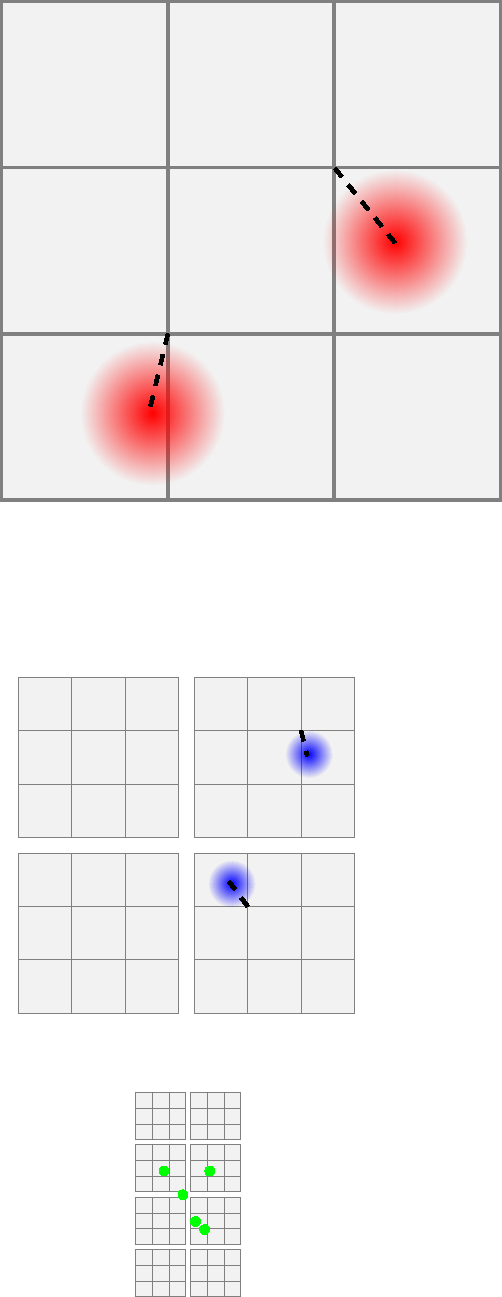
\includegraphics[width=0.25\textwidth]{61_pidt/dual-tree.pdf}
\end{center}

\noindent
A tree with three levels.
Particles with a large cut-off radius (red) are held on rather coarse levels.
Particles with very small cut-off are sorted (dropped) into the fine grid
levels.
Each particle is always associated to its closest vertex (dotted line).
It is the mesh which holds (owns) the vertices.
The toolset's predefined action set can automatically maintain/update these
associations after each grid sweep.
It also moves particles up and down the grid hierarchy if the particles' cut-off
radius changes or the grid changes.



\begin{definition}
  Our storage is vertex-oriented whereas most particle literature stores
  particles within cells.
  If we think of a dual multiscale mesh, i.e.~a mesh that is shifed by $h/2$
  alon each coordinate axis, then \Peano's approach also works with cells.
  Such shifted meshes are often called \emph{dual} meshes and I therefore speak
  of a \emph{dual tree}.
\end{definition}



\section{Particle-particle interaction}


\Peano\ always runs through the mesh top-down, i.e.~it traverses the spacetree
in a depth-first fashion.


Per cell, the code assembles a \texttt{local set}. 
This is a list of pointers to those particles that are associated to a cell's
$2^d$ vertices.
With the local set, you can make particles held on one resolution level
interact with each other.
You get an cubic area of $2h$ side-lenght per cell:
As a particle is always associated to its closest vertex, the local set holds all particles whose cut-off radius overlap with the cell. 


Adaptivity and particles with different cut-off are not yet captured through the
local set notion.
There's thus a second set that I call active set. 
The active set is the local set plus all local sets that have been active on
coarser levels within the tree.


If you use the \texttt{toolbox.particles.ParticleParticleInteraction} action
set, you pass it some C source code that works with the particles.
This C code has access to three variables: the active set, the local set and the
cell marker (of type \linebreak \texttt{peano4::datatraversal::CellMarker}).
Let's assume that each particle carries some velocity and that we could cut-off
gravity---which we clearly should not.


The straightforward particle-particle interaction then looks conceptionally as
follows:

\begin{code}
// Run over local set
for (auto& p: localParticles) {
  // Pick only those particles that reside within the current cell, otherwise
  // we would update each particle up to 2^d times. I do not exploit the
  // symmetry of forces here
  if ( marker.isContained( p->getX() ) ) {
    for (auto& pp: activeParticles) {
      // No interaction with particle itself
      if (p!=pp) {
        tarch::la::Vector<Dimensions,double> dist = pp->getX() - p->getX();
        [...]
      }
    }
  }
}
\end{code}




\section{Further action sets}

There are a few further action sets in the toolbox that help you to write your
Lagrangian code:


\begin{enumerate}
  \item The action set \texttt{toolbox.particles.UpdateParticleGridAssociation}
  is the core set. You'll always need this one to get the mapping of
  vertices/cells to particles right. The mapping is written in a way that it
  allows for \emph{tunnelling}, i.e.~particles may move more than one cell per
  grid sweep. In return, it is not necessary to update the particles in each and
  every time step---if your physics supports this.
  \item The action set \texttt{toolbox.particles.PlotParticlesInVTKFormat}
  provides a basic particle plotter which dumps particles, their cut-off radius
  plus their particle-vertex associativity. If you have to dump further
  properties, you have to write your own plotter. The generated plotter however
  can serve as a blueprint.
  \item The action set \texttt{toolbox.particles.ParticleTreeAnalysis} provides
  some fundamental tree analysis such as a multiscale counting how many
  particles reside within each cell. You'll need some additional data structures
  (per cell) to use this action set.
  \item The action set \texttt{toolbox.particles.ParticleAMR} uses the tree
  analysis to guide dynamic grid adaptivity. You can specify how many particles
  are held per cell at least, e.g., while the cut-off radius feeds naturally
  into the AMR.
\end{enumerate}


\section*{Links and further reading}

\begin{itemize}
  \item The ``official'' pidt paper is
{\tiny \begin{verbatim}
@article{WEINZIERL201642,
title = "Two particle-in-grid realisations on spacetrees",
journal = "Parallel Computing",
volume = "52",
pages = "42 - 64",
year = "2016",
issn = "0167-8191",
doi = "https://doi.org/10.1016/j.parco.2015.12.007",
url = "http://www.sciencedirect.com/science/article/pii/S0167819115001635",
author = "T. Weinzierl and B. Verleye and P. Henri and D. Roose",
keywords = "Particle-in-cell, Spacetree, Particle sorting, AMR, Lagrangian–Eulerian methods, Communication-avoiding"
}  \end{verbatim}}
  If you use the software, it would be great if you could cite this one.
\end{itemize}



 \newpage
 \chapter{\Peano\ PETSc}
\label{chapter:petsc}




 \part{Examples: Using the high-level Python API}
 \newpage
 \chapter{A geometric-algebraic multigrid solver}
\label{section:python-api-examples:multigrid}

All the examples from this chapter can be found in Peano's
\texttt{python/examples} directory.


\section{A matrix-free Jacobi smoother with rediscretisation}

\begin{remark}
 This example corresponds to the \texttt{matrix-free.py} script.
\end{remark}



\section{A parallel version of the code}

\begin{remark}
 This example corresponds to the \texttt{amr-parallel.py} script.
\end{remark}

For the time being, we again keep stuff pretty simple.
We stick to a regular grid, create this grid serially on one rank or core, 
and then distribute it.
That is, we don't do any load balancing and, as long as the grid remains 
stationary, we will have a brilliant balancing.
For the remainder, the text will use rank/core/partition as synonyms.
Peano 4 does not distinguish between them, i.e.~it uses domain decomposition
to keep both ranks and threads busy.


The first step to integrate multicore parallelisation---I always recommend to
start with multithreading first and then to add MPI on top---is to set an
appropriate number of threads.
Different to OpenMP, Peano requires the user to configure the thread count
within the code. 
This is done via the configuration method of the singleton
\texttt{tarch::multicore::Core}\footnote{Peano's C++14 multithreading variant
at the moment does not allow you to set the thread count, as C++ offers no such
feature. I therefore recommend TBB.}.


To split up a tree, you have to call
\begin{code}
  peano4::parallel::SpacetreeSet::getInstance().split(mytreeNumber,cellsPerCore,destinationRank)
\end{code}
\noindent
on your rank. This operation wants to know which spacetree to split, how many
cells to cut from it (we always count fine grid cells), and to which rank to
deploy the split tree.
The operation establishes a logical tree topology on the spacetrees, as we
always start with tree number 0 on rank 0 and then fork and fork and fork.
Joins are currently not supported by Peano 4's API: the code automatically fuses
trees if they degenerate.


After each split, you need at least two iterations to actually realise it, as 
Peano has to move the data, update all data meta information, and so forth. 
The iterations (grid sweeps) are no special ones, i.e.~you can continue to
compute.
It is just reasonable to keep in mind that after a split of a rank, this rank
will not be able to do any further domain decomposition for a few more sweeps
until it has ``recovered''. 
Likewisely, new trees will not enter the game immediately, but with a 1--2
iterations delay.
If you want to avoid that computations and domain decomposition intermix, you
can add code snippets alike

\begin{code}
int cellsPerCore = peano4::parallel::SpacetreeSet::getInstance().getGridStatistics().getNumberOfLocalUnrefinedCells() / coreCount;
logInfo( "main()", "should host " << cellsPerCore << " cells per core" );

for (int thread=1; thread<coreCount; thread++) {
  if ( not peano4::parallel::SpacetreeSet::getInstance().split(0,cellsPerCore,0)) { 
   logWarning( "runParallel(...)", "failed to assign thread " << thread << " " << cellsPerCore << " cell(s)" ); 
  }
}
\end{code}

\noindent
This is however your decision. Peano does not impose any constraints on you that
you have to separate load balancing, load re-distribution and computations.


\section{A parallel AMR Jacobi solver}

\begin{remark}
 This example corresponds to \texttt{amr-parallel.py} script, too.
\end{remark}

 \newpage
 \chapter{A finite volumes code}
\label{section:python-api-examples:finite-volumes}

We create a simple Finite Volumes solver here.
The examples starts with a simple regular grid, parallelises this grid, and
finally adds adaptive mesh refinment (AMR).
It employs a block-structured formalism and relies heavily on premanufactured
actions and solver ingredients from the ExaHyPE2/ExaClaw project.


\section{Setting up the data structures}

We model our grid as an AMR grid consisting of $N \times N$ blocks.
We call these blocks \emph{patches}.
In the example below, we have chosen $N=7$.
In general, odd choices of $N$ are advantageous once you enable AMR as we will
discuss later.

\begin{center}
  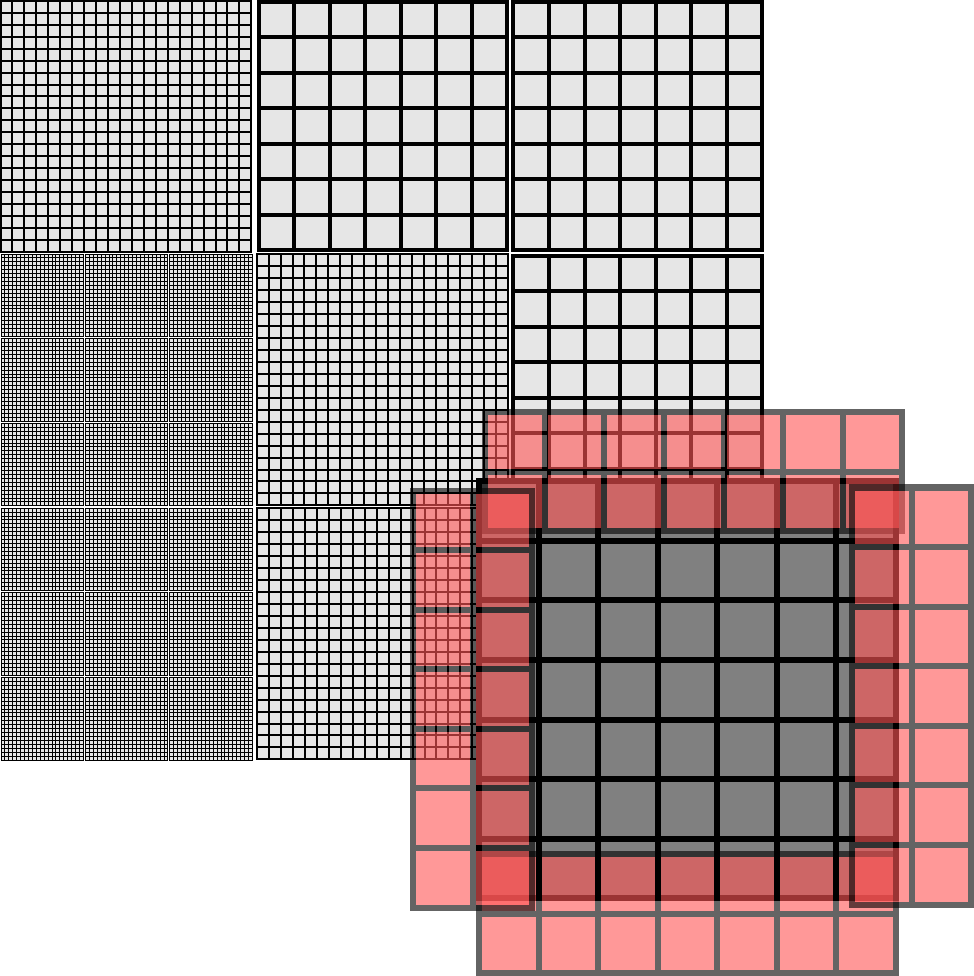
\includegraphics[width=0.6\textwidth]{42_finite-volumes/block-structured.pdf}
\end{center}

\begin{code}
project = peano4.Project( ["examples", "finitevolumes"], "." )
patch_size = 7
unknowns   = 5
patch = peano4.datamodel.Patch( (patch_size,patch_size,patch_size), unknowns, "Q" )
project.datamodel.add_cell(patch)
\end{code}

\noindent
In the above example, every voxel within the $N \times N$ patches holds five
unknowns.
In general, I prefer the term voxel here, as cell again is ambigous given that
we construct the Peano4 host mesh from cells.


With one patch per cell, we could traverse the mesh and do something per cell.
This however is of limited value.
We have to couple the phenomena what is going on in neighbouring cells.
Peano realises a strict element-wise traversal, i.e.~there's no way to access
the neighbour cell of a cell directly.
However, we can hijack the faces.


The idea here is that we embed a $2 \times N$ ($d=2$) or $2 \times N \times N$
($d=3$), respectively, patch into each face. 
Let this auxiliary patch overlap the adjacent cells.
Then, we effectively have a halo of one cell available within each cell:
We know the cell data. 
We also have access to the $2d$ faces where each hosts a degenerated patch.
One later of this patch is a copy of our own data, i.e.~does not give us
additional information.
The other layer of the auxiliary patch however holds data from the neighbour.
It gives us information from the neighbour patch.


In theory, we could only replicate those quantities that we really need. 
But it makes our live easier to just hold all five quantities in the auxiliary
face data structures, too:

\begin{code}
patch_overlap = peano4.datamodel.Patch( (2,patch_size,patch_size), unknowns, "Q" )
project.datamodel.add_face(patch_overlap)
\end{code}


Before we generate the code, we export some of the Python constants that we use
into C/C++, so we have it available there, too:

\begin{code}
project.constants.export( "PatchSize", patch_size )
project.constants.export( "NumberOfUnknownsPerCell", unknowns )
\end{code}


\section{Administration of the data structures}

Projecting the patches onto the face data structures and back is a mechnical
task.
Therefore, Peano4 offers a toolbox to relieve you from the pain to 
recode it over and over again.
Using this toolbox, you add the projections to your algorithmic steps, and the
API then automatically injects these features (aspects) into your code:

\begin{code}
perform_time_step      = peano4.solversteps.Step( "TimeStep" )
perform_time_step.use_cell(patch)
perform_time_step.use_face(patch_overlap)
...
perform_time_step.add_action_set( 
  peano4.toolbox.blockstructured.ReconstructPatchAndApplyFunctor(patch,patch_overlap,...)
) 
perform_time_step.add_action_set( 
  peano4.toolbox.blockstructured.ProjectPatchOntoFaces(patch,patch_overlap) 
)
\end{code}



\begin{center}
  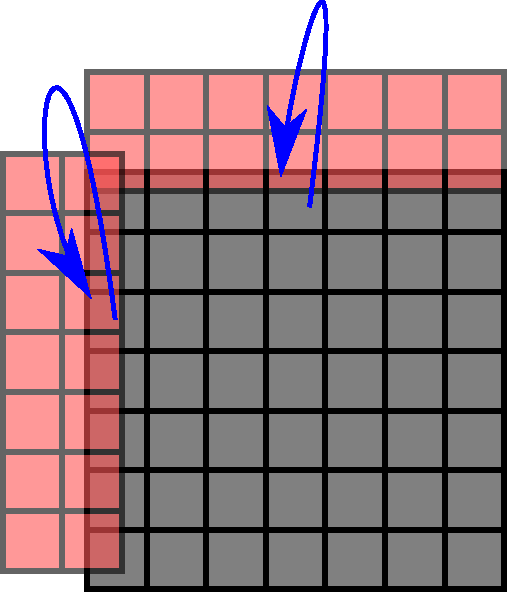
\includegraphics[width=0.3\textwidth]{42_finite-volumes/ProjectPatchOntoFaces.pdf}
\end{center}


\noindent
The image above illustrates what \texttt{ProjectPatchOntoFaces} does:
It knows the dimensions of both the patches and the face auxiliary data
structures and thus can ensure that the right data is copied from the cell into
the $2^d$ faces when we leave a cell throughout the grid traversal.



The action set \texttt{ReconstructPatchAndApplyFunctor} works slighlty different
yet can be read, from a patch projection point of view, as transpose of
\texttt{ProjectPatchOntoFaces}:
It creates a auxiliary variable \texttt{reconstructedX} with X being the name
you gave the Unknowns of the patch.
This auxiliary variable has the dimensions 
$N+2 \times N+2 \times N+2$\footnote{All tools work with overlaps greater than
2. But to keep the text simple, I stick to 2.}.
It then copies over the patch data into this auxiliary patch and uses the faces
to supplement it with halo data around it.
So that it, you get the original patch data plus the cells around it in one big
patch.


\section{A manually implemented FV scheme}

As the name suggests, the reconstruction step is typically combined with the
invocation of some computation on the patch.
We give a simple example of a Finite Volume solver for the Euler equations here.


Once a patch is reconstructed, we have a huge double array (AoS) of the
reconstructed patch, i.e.~the patch plus its surrounding halo, available.
It holds a copy of the actual patch data.
This patch data is still available as well, so we can use the reconstructed
array as a preimage and write any outcome into the patch data structure.


We begin with defining a simple functor implementing this PDE plus a very simple
Rusanov flux:
\begin{code}
auto eigenvalues = [](double Q[5], const tarch::la::Vector<Dimensions,double>& x, 
  int normal, double lambda[5]
) -> void {
  constexpr double gamma = 1.4;
  const double irho = 1./Q[0];
  #if Dimensions==3
    const double p = (gamma-1) * (Q[4] - 0.5*irho*Q[1]*Q[1]+Q[2]*Q[2]+Q[3]*Q[3]);
  #else
    const double p = (gamma-1) * (Q[4] - 0.5*irho*Q[1]*Q[1]+Q[2]*Q[2]);
  #endif

  const double u_n = Q[normal + 1] * irho;
  assertion10( gamma * p * irho>=0.0, gamma, p, irho, x, normal, Q[0], Q[1], Q[2], Q[3], Q[4] );
  const double c   = std::sqrt(gamma * p * irho);

  lambda[0]  = u_n;
  lambda[1]  = u_n;
  lambda[2]  = u_n;
  lambda[3]  = u_n + c;
  lambda[4]  = u_n - c;
    
  assertion4( lambda[0]==lambda[0], u_n, c, x, normal );
  assertion4( lambda[1]==lambda[1], u_n, c, x, normal );
  assertion4( lambda[2]==lambda[2], u_n, c, x, normal );
  assertion4( lambda[3]==lambda[3], u_n, c, x, normal );
  assertion4( lambda[4]==lambda[4], u_n, c, x, normal );
};
  
auto flux = [](
  double Q[5], const tarch::la::Vector<Dimensions,double>& x, int normal, double F[5]
) -> void {
  assertion5( Q[0]==Q[0], Q[0], Q[1], Q[2], Q[3], Q[4] );    
  assertion5( Q[1]==Q[1], Q[0], Q[1], Q[2], Q[3], Q[4] );    
  assertion5( Q[2]==Q[2], Q[0], Q[1], Q[2], Q[3], Q[4] );    
  assertion5( Q[3]==Q[3], Q[0], Q[1], Q[2], Q[3], Q[4] );    
  assertion5( Q[4]==Q[4], Q[0], Q[1], Q[2], Q[3], Q[4] );    
    
  assertion5( Q[0]>1e-12, Q[0], Q[1], Q[2], Q[3], Q[4] );
  constexpr double gamma = 1.4;
  const double irho = 1./Q[0];
  #if Dimensions==3
    const double p = (gamma-1) * (Q[4] - 0.5*irho*Q[1]*Q[1]+Q[2]*Q[2]+Q[3]*Q[3]);
  #else
    const double p = (gamma-1) * (Q[4] - 0.5*irho*Q[1]*Q[1]+Q[2]*Q[2]);
  #endif

  switch (normal) {
    case 0:
      {
        F[0] = Q[1];
        F[1] = irho*Q[1]*Q[1] + p;
        F[2] = irho*Q[2]*Q[1];
        F[3] = (Dimensions==3) ? irho*Q[3]*Q[1] : 0.0;
        F[4] = irho*(Q[4]+p)*Q[1];
      }
      break;
    case 1:
      {
        F[0] = Q[2];
        F[1] = irho*Q[1]*Q[2];
        F[2] = irho*Q[2]*Q[2] + p;
        F[3] = (Dimensions==3) ? irho*Q[3]*Q[2] : 0.0;
        F[4] = irho*(Q[4]+p)*Q[2];
      }
      break;
    case 2:
      {
        F[0] = Q[3];
        F[1] = irho*Q[1]*Q[3];
        F[2] = irho*Q[2]*Q[3];
        F[3] = (Dimensions==3) ? irho*Q[3]*Q[3] + p : 0.0;
        F[4] = irho*(Q[4]+p)*Q[3];
      }
      break;
  }

  assertion( F[0]==F[0] );
  assertion( F[1]==F[1] );
  assertion( F[2]==F[2] );
  assertion( F[3]==F[3] );
  assertion( F[4]==F[4] );
};

auto splitRiemann1d = [&flux, &eigenvalues](
  double QL[5], double QR[5], const tarch::la::Vector<Dimensions,double>& x,
  double dx, double dt, int normal, double F[5]
) -> void { double averageQ[5]; 
  for (int unknown=0; unknown<5; unknown++) {
    averageQ[unknown] = 0.5 * (QL[unknown] + QR[unknown]);    
  }
    
  double averageF[5];
  double lambdas[5];
  flux(averageQ,x,normal,averageF);
  
  double lambdaMax = 0.0;
  eigenvalues(averageQ,x,normal,lambdas);
  for (int unknown=0; unknown<5; unknown++) {
    lambdaMax = std::max(lambdaMax,lambdas[unknown]);
  }
  
  for (int unknown=0; unknown<5; unknown++) {
    F[unknown] = averageF[unknown] - 0.5 * lambdaMax * (QR[unknown] - QL[unknown]);
  }
};  
\end{code}

\noindent
Let all of this be one string assigned to a variable \texttt{functor}.


So this string now contains all the helpers we need to realise a Finite Volume
scheme, but it does not yet implement the scheme itself.
This is the final loop that's missing, and we can directly attach it to the
functor and then pass over to the reconstruction aspect:

\begin{code}
  constexpr int PatchSize = 13;
  constexpr int HaloSize  = 1;    
  double dt = 0.0001;
  assertion( dx>=tarch::la::NUMERICAL_ZERO_DIFFERENCE );
  dfor(cell,PatchSize) { // DOFS_PER_AXIS
    tarch::la::Vector<Dimensions,double> voxelCentre = centre 
                                           - static_cast<double>((PatchSize/2+HaloSize)) * tarch::la::Vector<Dimensions,double>(dx)
                                           + tarch::la::multiplyComponents(cell.convertScalar<double>(), tarch::la::Vector<Dimensions,double>(dx));
    
    tarch::la::Vector<Dimensions,int> currentVoxel = cell + tarch::la::Vector<Dimensions,int>(HaloSize); // OVERLAP / Halo layer size
    int currentVoxelSerialised = peano4::utils::dLinearised(currentVoxel,PatchSize + 2*HaloSize);
    
    double accumulatedNumericalFlux[] = { 0.0, 0.0, 0.0, 0.0, 0.0 };
  ...
  }
\end{code}



\section{ExaHyPE's solvers}

Writing all the Finite Element core routines manually is a tedious and
time-consuming process.
It is convenient to go through an ExaHyPE project instead.
To do so, please ensure that your configure script has been passed the
\texttt{--with-exahype} command.


tedious.


% 
% import peano4.visualisation
% import peano4.toolbox


 
 
 \part{Low level (C/C++) programming}
 
\noindent
\Peano's core is a plain C++ application using MPI plus a shared memory
library.
It can add support for HDF5, vtk, and so forth;
depends how your code is configured.
These underlying libraries/APIs are hidden away from user code by the core.
At the same time, we provide a Python API which hides away most of the core.
At one point, you will however be required to program \Peano\ directly with C++. 


% While I document some of the C++ rationale and ideas as well as features, most
% users can first safely discuss all the C++ chapters and directly jump to the
% application examples which are modelled through the Python interface.
 
 
\section*{Generic structure of a \Peano\  application}

Though I do not tell users exactly how to write their code, there's some kind of
generic structure that is common to all Peano simulations.
We can consider it to be some kind of pattern/best practice.


First, we distinguish the global master---typically rank 0---and all the other
ranks.
It is the global master that makes all the decisions and hosts the main logic.
It tells the other ranks what to do in each step. 
Typical actions are
\begin{itemize}
  \item run through your mesh once,
  \item split up the domain (though each rank can decide to do this totally
  independently),
  \item plot some data, or, eventually,
  \item terminate.
\end{itemize}


Therefore, the global master basically sets a counter/id which uniquely
identifies which step to run next.
It then says ``go ahead'' and runs this step itself.
All the other ranks are noticed (via an internal broadcast in the core) which
step to run, do the same thing, and then wait for the next wake-up call.
At the end, the global master sets the id of a terminate.
As all the ranks loop until they receive this terminate id, they do go down as
well in the end.


A typical main thus looks as follows
\begin{code}
  if (tarch::mpi::Rank::getInstance().isGlobalMaster() ) {
    while ( selectNextAlgorithmicStep() ) {
      step();
    }
  }
  else {
    while (peano4::parallel::Node::getInstance().continueToRun()) {
      step();
    }
  }
\end{code}


\noindent
where the routine \texttt{selectNextAlgorithmicStep()} issues one call of
\begin{code}
peano4::parallel::Node::getInstance().setNextProgramStep(myStepNumber);
\end{code}

The \texttt{step()} routine then is usually a big switch statement:
\begin{code}
int stepIdentifier = peano4::parallel::Node::getInstance().getCurrentProgramStep();
switch (stepIdentifier) {
  case 0:
    {
      observers::CreateGrid  observer;
      peano4::parallel::SpacetreeSet::getInstance().traverse(observer);
    }
    break;
  case 1:
    {
      // split up domain
    }
}
\end{code}


\noindent
Nothing stops you from triggering multiple traversals (or none at all) within a
step.


\begin{remark}
 On the highest level, Peano4 implements a BSPish structure where the global
 rank issues a step and then all ranks run this step simultaneously. You can
 however define the notion of a superstep, i.e.~make one superstep issue
 multiple grid traversals. It is just important that all spacetree sets do
 exactly the same number of iterations.
\end{remark}


\noindent
The numbers within the case statements are kind of magic constants and you can
redefine them. 
However, I recommend to read the documentation of \texttt{setNextProgramStep()}
(there are some predefined constants that you should not use), and I recommend
that you use the predefined enums in \texttt{observers::StepRepository} if you
work with the Python API, too.
In this repository, there are predefined integers for all of the algorithm steps
you've defined. 


With the above structure, the Peano execution trace is close to trivial:
You simply run through your grid $n$ times and after each step, the core
exchanges all of the data.


\section*{MPI and shared memory programming}

If you run Peano4 with MPI, you buy into MPI's SPMD paradigm, i.e.~every single
rank hosts one instance of Peano.
Each Peano instance in return hosts multiple subspacetrees, i.e.~multiscale
domain partitions.
It is the user's responsibility to ensure that the ranks do coordinate with each
other.
That is, the user has to ensure that whenever you run a certain type of grid
sweep on one rank, then the other ranks run this sweep as well.
For this, each rank has to host one spacetree set, and these sets have to be
configured with the same parameters (domain offset plus domain size).
I do provide Python interfaces/APIs to model this behaviour, but it might be
reasonable to understand how it works.



A typical Peano4 code distinguishes the global master (rank 0) from the workers
(all other ranks).
The global master hosts all the program logic, i.e.~decides which steps to run
in which order.
There's no reason for you not to emancipate from this pattern, but it has proven
of value.
The main of this pattern always looks similar to 
\begin{code}
  if (tarch::mpi::Rank::getInstance().isGlobalMaster() ) {
    // All the program logic, i.e. all decisions here
  }
  else {
    // React to decisions what to do next on all other ranks
  }
\end{code}


Before we start, lets assume that each individual step (type of run through the
mesh) has a unique positive number. 

A typical parallel grid sweep looks as follows:
\begin{enumerate}
  \item 
\end{enumerate} 



\subsection{Realising a domain decomposition}

This is a howto for domain decomposition. 
For details about the underlying algorithmics and design decisions, please
consult Chapter \ref{section:design:domain-decomposition}.
As mentioned in various places, Peano does not fundamentally distinguish shared
memory and distributed memory parallelisation unless you work explicitly with
tasks.
That is, all split remarks here do also apply to shared memory.


Peano's core domain decomposition contact point is the singleton
\texttt{SpacetreeSet} on each compute node (rank).
You can tell this set to decompose one of the local spacetrees further through
its \texttt{split} routine.
After each split, the involved spacetrees need at least two iterations to
``recover'' before they are available for further spilts.


Split accepts the number of fine grid cells that are two be given away to
another rank.
The domain decomposition follows the Peano space-filling curve.
If $3^d$ cells along this curve are to be deployed to a different rank, then
Peano also deploys the parent of this $3^d$ assembly to a remote rank.
With dynamic AMR (or throughout an initial grid construction), it can happen
that Peano runs into a cell that is to be moved over to another rank and is
refined at the same time.
In this case, the cell plus all of its children is deployed.


\begin{remark}
 Splits imply that some spacetree data has to be copied and (temporarily) is
 held redundantly. In principle, you can issue as many splits in one rush as you
 like. In practice, it often makes sense to constrain the maximum number of
 splits issued per grid traversal. This ensures that you don't run out of
 memory. Also, splits require the Peano core to run some steps serially. 
 So also from a time-to-solution point of view, limiting the number of splits
 (in particular if they affect the same rank) is a good idea.
\end{remark}



The issue with (real) dynamic AMR is that it is very difficult to know how many
cells will be around after a grid sweep.
The same holds for the grid construction.
For runtime and memory reasons, you don't want to build up the grid completely
before you start to decompose it.
The following realisation pattern has turned out to be advantageous:
\begin{itemize}
  \item Build up an initial grid on the first rank up to a certain, reasonable,
  grid level. It should host at least $3^d \cdot r$ fine grid cells if you have
  $r$ ranks. This seems to be a reasonable rule of thumb.
  \item Split up this initial grid into $r$ spacetrees where each spacetrees is
  associated with a node of its own.
  \item Wait for one tree traversal, i.e.~run through the grid without adding
  further mesh elements. This ensures that the distributed mesh has been
  migrated completely before we continue.
  \item Continue to build up the grid.
  \item Compute a good guess how many cells should roughly end up per core.
  Store this guess.
  \item While the grid is constructed, decompose it further.
  \item Once the grid is complete, recompute how many cells should end up per
  core. Split up all the trees that are too big further and distribute these
  further trees among the ranks.
\end{itemize}



\begin{remark}
Irgendwie darf man net 2x traverse aufrufen in meinem Code. Evtl. liegt das aber
auch am Datenaustausch. Aber ist halt einfach bad smell in meinem Code!
\end{remark}

 

 \newpage
 \chapter{Guiding principles, high-level concepts and design decisions}


\section{Generic structure of a \Peano\  application}

Though I do not tell users exactly how to write their code, there's some kind of
generic structure that is common to all Peano simulations.
We can consider it to be some kind of pattern/best practice.


First, we distinguish the global master---typically rank 0---and all the other
ranks.
It is the global master that makes all the decisions and hosts the main logic.
It tells the other ranks what to do in each step. 
Typical actions are
\begin{itemize}
  \item run through your mesh once,
  \item split up the domain (though each rank can decide to do this totally
  independently),
  \item plot some data, or, eventually,
  \item terminate.
\end{itemize}


Therefore, the global master basically sets a counter/id which uniquely
identifies which step to run next.
It then says ``go ahead'' and runs this step itself.
All the other ranks are noticed (via an internal broadcast in the core) which
step to run, do the same thing, and then wait for the next wake-up call.
At the end, the global master sets the id of a terminate.
As all the ranks loop until they receive this terminate id, they do go down as
well in the end.


A typical main thus looks as follows
\begin{code}
  if (tarch::mpi::Rank::getInstance().isGlobalMaster() ) {
    while ( selectNextAlgorithmicStep() ) {
      step();
    }
  }
  else {
    while (peano4::parallel::Node::getInstance().continueToRun()) {
      step();
    }
  }
\end{code}


\noindent
where the routine \texttt{selectNextAlgorithmicStep()} issues one call of
\begin{code}
peano4::parallel::Node::getInstance().setNextProgramStep(myStepNumber);
\end{code}

The \texttt{step()} routine then is usually a big switch statement:
\begin{code}
int stepIdentifier = peano4::parallel::Node::getInstance().getCurrentProgramStep();
switch (stepIdentifier) {
  case 0:
    {
      observers::CreateGrid  observer;
      peano4::parallel::SpacetreeSet::getInstance().traverse(observer);
    }
    break;
  case 1:
    {
      // split up domain
    }
}
\end{code}


\noindent
Nothing stops you from triggering multiple traversals (or none at all) within a
step.


\begin{remark}
 On the highest level, Peano4 implements a BSPish structure where the global
 rank issues a step and then all ranks run this step simultaneously. You can
 however define the notion of a superstep, i.e.~make one superstep issue
 multiple grid traversals. It is just important that all spacetree sets do
 exactly the same number of iterations.
\end{remark}


\noindent
The numbers within the case statements are kind of magic constants and you can
redefine them. 
However, I recommend to read the documentation of \texttt{setNextProgramStep()}
(there are some predefined constants that you should not use), and I recommend
that you use the predefined enums in \texttt{observers::StepRepository} if you
work with the Python API, too.
In this repository, there are predefined integers for all of the algorithm steps
you've defined. 


With the above structure, the Peano execution trace is close to trivial:
You simply run through your grid $n$ times and after each step, the core
exchanges all of the data.


\section{MPI and shared memory programming}

If you run Peano4 with MPI, you buy into MPI's SPMD paradigm, i.e.~every single
rank hosts one instance of Peano.
Each Peano instance in return hosts multiple subspacetrees, i.e.~multiscale
domain partitions.
It is the user's responsibility to ensure that the ranks do coordinate with each
other.
That is, the user has to ensure that whenever you run a certain type of grid
sweep on one rank, then the other ranks run this sweep as well.
For this, each rank has to host one spacetree set, and these sets have to be
configured with the same parameters (domain offset plus domain size).
I do provide Python interfaces/APIs to model this behaviour, but it might be
reasonable to understand how it works.



A typical Peano4 code distinguishes the global master (rank 0) from the workers
(all other ranks).
The global master hosts all the program logic, i.e.~decides which steps to run
in which order.
There's no reason for you not to emancipate from this pattern, but it has proven
of value.
The main of this pattern always looks similar to 
\begin{code}
  if (tarch::mpi::Rank::getInstance().isGlobalMaster() ) {
    // All the program logic, i.e. all decisions here
  }
  else {
    // React to decisions what to do next on all other ranks
  }
\end{code}


Before we start, lets assume that each individual step (type of run through the
mesh) has a unique positive number. 

A typical parallel grid sweep looks as follows:
\begin{enumerate}
  \item 
\end{enumerate} 



\subsection{Realising a domain decomposition}

This is a howto for domain decomposition. 
For details about the underlying algorithmics and design decisions, please
consult Chapter \ref{section:design:domain-decomposition}.
As mentioned in various places, Peano does not fundamentally distinguish shared
memory and distributed memory parallelisation unless you work explicitly with
tasks.
That is, all split remarks here do also apply to shared memory.


Peano's core domain decomposition contact point is the singleton
\texttt{SpacetreeSet} on each compute node (rank).
You can tell this set to decompose one of the local spacetrees further through
its \texttt{split} routine.
After each split, the involved spacetrees need at least two iterations to
``recover'' before they are available for further spilts.


Split accepts the number of fine grid cells that are two be given away to
another rank.
The domain decomposition follows the Peano space-filling curve.
If $3^d$ cells along this curve are to be deployed to a different rank, then
Peano also deploys the parent of this $3^d$ assembly to a remote rank.
With dynamic AMR (or throughout an initial grid construction), it can happen
that Peano runs into a cell that is to be moved over to another rank and is
refined at the same time.
In this case, the cell plus all of its children is deployed.


\begin{remark}
 Splits imply that some spacetree data has to be copied and (temporarily) is
 held redundantly. In principle, you can issue as many splits in one rush as you
 like. In practice, it often makes sense to constrain the maximum number of
 splits issued per grid traversal. This ensures that you don't run out of
 memory. Also, splits require the Peano core to run some steps serially. 
 So also from a time-to-solution point of view, limiting the number of splits
 (in particular if they affect the same rank) is a good idea.
\end{remark}



The issue with (real) dynamic AMR is that it is very difficult to know how many
cells will be around after a grid sweep.
The same holds for the grid construction.
For runtime and memory reasons, you don't want to build up the grid completely
before you start to decompose it.
The following realisation pattern has turned out to be advantageous:
\begin{itemize}
  \item Build up an initial grid on the first rank up to a certain, reasonable,
  grid level. It should host at least $3^d \cdot r$ fine grid cells if you have
  $r$ ranks. This seems to be a reasonable rule of thumb.
  \item Split up this initial grid into $r$ spacetrees where each spacetrees is
  associated with a node of its own.
  \item Wait for one tree traversal, i.e.~run through the grid without adding
  further mesh elements. This ensures that the distributed mesh has been
  migrated completely before we continue.
  \item Continue to build up the grid.
  \item Compute a good guess how many cells should roughly end up per core.
  Store this guess.
  \item While the grid is constructed, decompose it further.
  \item Once the grid is complete, recompute how many cells should end up per
  core. Split up all the trees that are too big further and distribute these
  further trees among the ranks.
\end{itemize}



\begin{remark}
Irgendwie darf man net 2x traverse aufrufen in meinem Code. Evtl. liegt das aber
auch am Datenaustausch. Aber ist halt einfach bad smell in meinem Code!
\end{remark}

 

\subsection{Global communication}

\Peano\ handles all (multiscale) boundary data transfer and data migration
within the mesh.
Everything not tied to the mesh is \emph{not} handled by \Peano.
That means there's not even a reduction of the grid statistics over MPI.
We do provide reduction and broadcast features however. 

 
 \newpage
 \section{Logging, tracing and assertions}
\label{section:logging}



% \chapterDescription
%   {
%     There are no real examples coming along with this chapter, but you might
%     want to use its topics for any project.
%   }
%   {
%     Chapter \ref{chapter:quickstart}.
%   }


%\subsection{The user interface}

%\subsection{Repository fields}

%\subsection{Logging}

Level
Was zum Chrome

 * - PeanoDebug = 1: Enable tracing
 * - PeanoDebug = 2: Enable assertions (includes level 1)
 * - PeanoDebug = 4: Enable debug messages (includes level 2)



Peano relies on a plain interface to write out user information. 
All constituents of this interface are collected in the package
\texttt{tarch::logging}.
Documentation on this package can be found in the corresponding header files,
files ending with \texttt{.doxys}, or the Peano webpage (section on sources).
The usage paradigm is simple:

\begin{enumerate}
  \item Each class that wants to write logging information requires an instance
  of class \texttt{tarch::logging::Log}. As such an instance is required per
  class, it makes sense to make this field a static one.
  \begin{code}
  #include "tarch/logging/Log.h"
  ...
  class MyClass {
    private:
      static tarch::logging::Log  _log;
  };
  
  tarch::logging::Log  MyClass::_log( "MyClass" );
  \end{code}
  For most auto-generated classes, the PDT already creates the \texttt{\_log}
  instance. Please keep to the nomenclature of the class field to make all
  macros work. Please use as string argument in the constructor the fully
  qualified class name.
  \item Whenever you want to log, you should use Log's' operations to write the
  messages. Alternatively, you may want to use the log macros from
  \texttt{Log.h}. They work with stringstreams internally, i.e.~you may write
  things along the lines
  \begin{code}
logInfo( "runAsMaster(...)", "time step " << i << ": dt=" << dt );
  \end{code}
  where you concatenate the stream with data.
\end{enumerate}

Peano offers three levels of logging:
\begin{itemize}
  \item {\textbf Info}. Should be used to inform your user about the application's
  state.
  \item {\textbf Warning}. Should be used to inform your user about bothering
  behaviour.
  The MPI code uses it, e.g., if many messages arrive in a different order than
  expected. Messages written to the warning level are piped to
  \texttt{cerr}.
  \item {\textbf Error}. Should be used for errors. Is piped to \texttt{cerr} as
  well.
  \item {\textbf Debug}. Should be used to write debug data. It goes to
  \texttt{cout} and all debug data is removed if you do not translate with the compile flag
  \texttt{-DDebug}. Notably, use the \texttt{logDebug} macros when you write to
  the debug level, as all required log operations then are removed by the
  compiler once you create a release version of your code.
\end{itemize}



\subsubsection{Logging device: CommandLineLogger}

The \texttt{Log} instance forwards the information to a logger. By default, this
is the \\ \texttt{tarch::logging::CommandLineLogger} which writes information
in a table-like format. You may want to write your own alternative
implementation of the logger if you require formats such as XML.

Alternatively, you can configure the command line logger to plot only those
fields that are of relevance to you.
For this, the logger provides a particular setter.
Please consult the header or the webpage for details on the semantics of the
arguments:
\begin{code}
tarch::logging::CommandLineLogger::getInstance().setLogFormat(
  " ", true, false, false, true, true, "my-fancy.log-file" );
\end{code} 

\noindent
This interface also allows you to pipe the output into a file rather than to the
terminal.
This is particular useful for MPI applications, as each rank is assigned a file
of its own and messages are not screwed up.
Typically, the logger is configured in the \texttt{main} of the application.

If you run Peano for long simulations and, notably, if you run Peano with debug
information switched on (\texttt{-DDebug}), log files soon become massive.
To ease the pain, Peano's command line logger offers an operation 
\begin{code}
tarch::logging::CommandLineLogger::getInstance().closeOutputStreamAndReopenNewOne();
\end{code} 
\noindent
that works if you have specified an output file before (see
\texttt{setLogFormat} above). Per close, you close all output files and start to
stream the output into a new file.
Typically, developers use this operation in their iterative schemes to stream
each iteration to a different file.
The output files are enumerated automatically.



\subsubsection{Log filter}

The amount of log information often becomes hard to track; notably if you run in
debug mode.
Often, you are interested only in a subset of all log messages.
For this, Peano offers log filters which provide a blacklist and whitelist
mechanism to filter messages before they are written.
A log filter entry is created by 
\begin{code}
    tarch::logging::CommandLineLogger::getInstance().addFilterListEntry( 
      ::tarch::logging::CommandLineLogger::FilterListEntry( 
        "debug", -1, "myproject", false ) );
\end{code} 
\noindent
and again this is something that is typically done in the \texttt{main}.
See the \texttt{CommandLineLogger} header for details on the log filters.


Configuring log filters in your source code is a convenient option when you
start a new project.
On the long run, it is cumbersome if you have to recompile every time you want
different log information.
Therefore, the \texttt{CommandLineLogger} also offers a routine that allows you
to load log filter entries from a text file.
This facilitates work with log filters.
The usage is straightforward
\begin{code}
tarch::logging::LogFilterFileReader::parsePlainTextFile( "my.log-filter" );
\end{code}

\noindent
and the format is very simple:
\begin{verbatim}
# Level  Trace    Rank   Black or white list entry
# (info or debug) (-1 means all ranks)
debug    tarch    -1     black
debug    peano    -1     black
info     tarch    -1     black
info     peano    -1     black
\end{verbatim}




\subsubsection{Tracing}

Peano uses tracing command in several places. 
Consult the mapping classes generated by the PDT, e.g. 
Tracing commands are basically debug statements, and once you compile your code
without \texttt{-DDebug} or with log filters on the debug level, tracing
messages are removed from the output.
In Peano, trace messages are used to track when a method is entered and when the
code leaves a routine.
They can be found all over the code.
The additional benefit of the trace routines compared to pure debug statements
is that the tracings also apply a well-suited indentation, i.e.~when you enter a
routine, all messages afterwards are indented by two spaces (default; can be
reconfigured) afterwards until you leave this operation again.


\begin{remark}
If you want to get familiar with the program workflow, you might want to use a
debugger to step to your program.
This is time consuming.
Another option is to configure your log filters such that only the trace
messages (debug messages) from the mapping are printed to the terminal/a file.
You can then run through this output and see which operations from the mapping
are called at which time.
\end{remark}



% \subsection{Using logging and tracing}

% \subsection{Statistics}

% \subsection{Assertions}



% vertex enumerator
 \newpage
 \chapter{Unit tests}
\label{section:test}


Peano introduces its own lightweight test concept with picks up best practices
from the JUnit world. 
While it is simple and has no external dependencies (all test routines are
collected within the \texttt{tarch} subdirectory), it provides a few macros to
handle numeric data---which might be convenient for AMR applications; so
there's some added value. It also provides test routines for vectors.


\section{Test architecture}

A Peano test is a class that implements and extends
\texttt{tarch::tests::TestCase}.
By convention, I place my tests always into subdirectories/subnamespaces of the
respective component, but this is not a must.
A test class must implement a \texttt{void run()} method.
This is the only convention. 
The Peano toolkit by default generates one (empty) test per project that can act
as a blueprint if you don't want to write your test manually. 
Feel free to delete the class if you don't want to write unit tests on your own
(though the test itself is empty and thus does not harm the test runs).

A proper test class should realise a couple of \texttt{void} operations without
arguments that run the individual tests.
A minimalistic test thus looks as follows:

\begin{code}
namespace myproject {
  namespace tests {
    class TestCase;
  }
}

class myproject::tests::TestCase : public tarch::tests::TestCase {
 private:
  /**
   * These operations implement the real tests.
   */
  void test1();
  void test2();
 public:
  TestCase();
  virtual ~TestCase();

  virtual void run();
};
\end{code}

\noindent
The test's \texttt{run} operation has to register the individual void
  routines running the actual tests:
  \begin{code}
void exahype::tests::TestCase::run() {
  testMethod(test1);
  testMethod(test2);
}
  \end{code}




\section{Running the tests}
Once these steps are handled, you can run the tests within your \texttt{main}.
For the core and tarch routines, I provide factory methods  

\begin{code}
tarch::getUnitTests();
peano4::getUnitTests();
\end{code}

\noindent
which deliver a test suite. To run them, I typically insert snippets alike
\begin{code}
  int unitTestsErrors = 0;
  tarch::tests::TestCase* tests = nullptr;

  tests = tarch::getUnitTests();
  tests->run();
  unitTestsErrors += tests->getNumberOfErrors();
  delete tests;
\end{code}

\noindent
into my main.
It returns an output similar to
\begin{code}
running test case collection "exahype2.tests.c" ...... ok                                                                                                                
running test case collection "exahype2.tests.solvers" .. ok                                                                                                              
running test case collection "exahype2.tests" .... ok                                                                                                                    
running test case collection "peano4.grid.tests" .................... ok                                                                                                 
running test case collection "peano4.grid"  ok                                                                                                                           
running test case collection "peano4.heap.tests" .. ok                                                                                                                   
running test case collection "peano4.heap"  ok                                                                                                                           
running test case collection "peano4"  ok                                                                                                                                
running test case collection "tarch"  ok                                                                                                                                
running global test case collection  ok                                                                                                                                 
\end{code}

\noindent
The output returns a hierarchical overview over all tests ran. 
The number of dots per package identifies the number of actual test functions in
a namespace.
If tests fail, the interface reports the exact location including file name and
line number.


\begin{remark}
  It is convenient to run tests only if you have translated your code with a 
  sufficient debug level (cmp.~Section \ref{section:logging}).
  When you write your own tests, I often add test attributes to the
  classes---fields that are not required but help me to validate object
  states. Since I protect these attributes with ifdefs reading Peano's debug
  level, they are removed from the production code.
\end{remark}



\section{Test routines}

A typical unit tests builds up some classes, befills them with data, invokes
some operations and finally checks the class state via some getters or routines
returning results.
Peano's way to do the actual tests are \texttt{validate} macros.
You find all these macros in the file \texttt{tarch/tests/TestMacros.h}.
There are three classes of macros:

\begin{itemize}
  \item Standard validation macros similar to assertions that test a boolean
  condition.
  \item Comparison macros that compare two values through the
  \texttt{operator==} (which might be overloaded).
  \item Comparison macros that compare doubles, vectors or matrices numerically,
  i.e.~up to a prescribed precision.
\end{itemize}

\noindent
All of these macros come along with variants that allow you to plot additional
information if a test has failed, i.e.~to plot the values of further variables,
e.g.
All validation macros automatically set a test to failed if they fail, and they
write a verbose message on the reason why some tests failed to the terminal.  



  Tests tend to become spaghetti code and some of them are very expensive to
  translate as the compiler's optimiser has a hard time to translate the long
  code fragments.
  I thus recommend to insert
  \begin{code}
#include "tarch/compiler/CompilerSpecificSettings.h"

#ifdef UseTestSpecificCompilerSettings
#pragma optimize("", off)
#endif

// All the implementation

#ifdef UseTestSpecificCompilerSettings
#pragma optimize("", on)
#endif
  \end{code}
  into your implementation file around all your code. This switches off all
  optimisation explicitly for the tests.



 \newpage
 \chapter{Further}
\label{section:logging}


\section{Logging, tracing and assertion architecture}

Peano is built upon a technical architecture (\texttt{tarch}) which provides
logging, tracing and assertions.
The two directory of relevance here is therefore \texttt{tarch/logging} plus the
file \texttt{Assertions.h}.
The latter file holds all the assertion macros, while the logging directory
holds a file \texttt{Log.h} which holds all of the essential logging and tracing
macros.


When we build Peano, we do distinguish different ``debug'' levels:
\begin{itemize}
  \item If a code is translated with \texttt{-DPeanoDebug=0}, all logging,
  tracing and assertion macros are disabled, i.e.~replaced by empty statements.
  Warning, information and error messages are still displayed.
  \item If a code is translated with \texttt{-DPeanoDebug=1}, all macros from
  \texttt{-DPeanoDebug=0} remain defined. This time however, all tracing
  functionality is enabled. With this mode, it is possible to do production
  runs plus to extract some performance data, e.g.
  \item If a code is translated with \texttt{-DPeanoDebug=2}, all the
  tracing macros from \texttt{-DPeanoDebug=1} remain defined. On top of this,
  Peano's assertions now are enabled, i.e.~assertion macros do not degenerate to
  nop but actually run tests. This might increase the runtime significantly yet
  the code permanently runs test.
  \item If a code is translated with \texttt{-DPeanoDebug=4}, logging and
  assertion macros from \texttt{-DPeanoDebug=4} remain defined. Furthermore, any
  debug information written through Peano's log interface is now not discarded
  (removed at compile time) but actually shown. This is the slowest mode
  yielding most of the data.
\end{itemize}



\section{Using the logging and tracing interface}

Peano relies on a plain interface to write out user information. 
All constituents of this interface are collected in the package
\texttt{tarch::logging}.
Documentation on this package can be found in the corresponding header files,
files ending with \texttt{.doxys}, or the Peano webpage (section on sources).
The usage paradigm is simple:

\begin{enumerate}
  \item Each class that wants to write logging information requires an instance
  of class \texttt{tarch::logging::Log}. As such an instance is required per
  class, it makes sense to make this field a static one.
  \begin{code}
  #include "tarch/logging/Log.h"
  ...
  class MyClass {
    private:
      static tarch::logging::Log  _log;
  };
  
  tarch::logging::Log  MyClass::_log( "MyClass" );
  \end{code}
%   For most auto-generated classes, the PDT already creates the \texttt{\_log}
%   instance. 
  Please keep to the nomenclature of the class field to make all
  macros work. Please use as string argument in the constructor the fully
  qualified class name. See the remarks on log filters below for an explanation
  for  this.
  \item Whenever you want to log, trace, write an error message or a warning,
  you should use Log's operations to write the messages. Alternatively, you may want to use the log macros from
  \texttt{Log.h}. They work with stringstreams internally, i.e.~you may write
  things along the lines
  \begin{code}
logInfo( "runAsMaster(...)", "time step " << i << ": dt=" << dt );
  \end{code}
  where you concatenate the stream with data.
\end{enumerate}

Peano offers four levels of logging through its macros:
\begin{itemize}
  \item {\bf Info}. Should be used to inform your user about the application's
  state.
  \item {\bf Warning}. Should be used to inform your user about bothering
  behaviour.
  The MPI code uses it, e.g., if many messages arrive in a different order than
  expected. Messages written to the warning level are piped to
  \texttt{cerr}.
  \item {\bf Error}. Should be used for errors. Is piped to \texttt{cerr} as
  well.
  \item {\bf Tracing}. Used to keep track of when a method is entered and
  then left again.
  \item {\textbf Debug}. Should be used to write debug data. It goes to
  \texttt{cout} and all debug data is removed if you do not translate with the compile flag
  \texttt{-DDebug}. Notably, use the \texttt{logDebug} macros when you write to
  the debug level, as all required log operations then are removed by the
  compiler once you create a release version of your code.
\end{itemize}



\section{Logging devices (formats)}

The \texttt{Log} instance forwards the information to a logger. By default, this
is the \\ \texttt{tarch::logging::ChromeTraceFileLogger}. You may want to write
your own alternative implementation or switch to another option.
Logging can be very time-consuming. I therefore decided to link the Log objects
to one particular log device statically. If you want to ``redirect'' your
outcome, you can either manually edit the logging header, or you can retranslate
your code with \texttt{-DUsedLogService=xxx}.
\texttt{xxx} is the class to be used.
I detail the variants I currently ship with Peano below.



\subsection{ChromeTraceFileLogger}

This logger writes the one json file per rank. The format conforms to Google
Chrome's tracing format, i.e.~you can open the file in Google Chrome by typing
in the URL \texttt{chrome:///tracing} and loading in the file in the GUI that
pops up.
As the format is prescribed, there are no opportunities to configure the output.
While the majority of all output data goes into these Chrome files, warnings,
errors and info messages are also dumped to the terminal in a format which can
be read by humans easily.



\subsection{CommandLineLogger}

Alternatively, you can ask Peano to dump all outcome in a human readable format.
This one can be tailored towards your needs.
For this, the logger provides a particular setter.
Please consult the header or the webpage for details on the semantics of the
arguments:
\begin{code}
tarch::logging::CommandLineLogger::getInstance().setLogFormat(
  " ", true, false, false, true, true, "my-fancy.log-file" );
\end{code} 

\noindent
The interface also allows you to pipe the output into a file rather than to the
terminal.
This is particular useful for MPI applications, as each rank is assigned a file
of its own and messages are not screwed up.
Typically, the logger is configured in the \texttt{main} of the application.

If you run Peano for long simulations and, notably, if you run Peano with debug
information switched on, log files soon become massive.
To ease the pain, Peano's command line logger offers an operation 
\begin{code}
tarch::logging::CommandLineLogger::getInstance().closeOutputStreamAndReopenNewOne();
\end{code} 
\noindent
that works if you have specified an output file before (see
\texttt{setLogFormat} above). Per close, you close all output files and start to
stream the output into a new file.
Typically, developers use this operation in their iterative schemes to stream
each iteration to a different file.
The output files are enumerated automatically.



\section{Log filter}

The amount of log information often becomes hard to track; notably if you run in
debug mode.
Often, you are interested only in a subset of all log messages.
For this, Peano offers log filters which provide a blacklist and whitelist
mechanism to filter messages before they are written.
A log filter entry is created by 
\begin{code}
tarch::logging::LogFilter::getInstance().addFilterListEntry( tarch::logging::LogFilter::FilterListEntry(
  tarch::logging::LogFilter::FilterListEntry::TargetInfo, 
  tarch::logging::LogFilter::FilterListEntry::AnyRank, "peano4", false
));
\end{code} 


\noindent
The log filter is a singleton, and log filters can be used totally independently
of the log output format.


Configuring log filters in your source code is a convenient option when you
start a new project.
On the long run, it is cumbersome if you have to recompile every time you want
different log information.
Therefore, the \texttt{CommandLineLogger} also offers a routine that allows you
to load log filter entries from a text file.
This facilitates work with log filters.
The usage is straightforward
\begin{code}
tarch::logging::LogFilterFileReader::parsePlainTextFile( "my.log-filter" );
\end{code}

\noindent
and the format is very simple:
\begin{verbatim}
# Level  Trace    Rank   Black or white list entry
# (info or debug) (-1 means all ranks)
debug    tarch    -1     black
debug    peano    -1     black
info     tarch    -1     black
info     peano    -1     black
trace    tarch    -1     black
trace    peano    -1     black
\end{verbatim}


\noindent
For performance reasons, it is important to take two facts into account:
\begin{enumerate}
  \item Black- and whitelisting works only on the class level. While tracing,
  logging, and so forth all tell you which operation has logged a certain entry,
  you cannot filter on the method level.
  \item Black- and whitelisting are not dynamic. The very first time a class
  wants to dump information, it queries the log filter. The result of the log
  filter then is hold persistently. 
\end{enumerate}



\section{Assertions}

Peano provides its own assertion format which is independent of C++ assertions.
Assertions are offered through macros, and if you choose a \texttt{PeanoDebug}
level which does not support assertions, then they are removed at compile time
from your code.

Peano's assertions interlink with the logging, i.e.~before they shut down a
rank, they ensure that all logs are flushed.
Furthermore, they provide a few convenient variations that 
\begin{enumerate}
  \item support numerical ``equality'' checks,
  \item support the logging of parameters, and
  \item support vector-valued comparisons.
\end{enumerate}

 \newpage
 \chapter{Synchronisation}
\label{section:synchronisation}


In \Peano, every rank holds a set of spacetrees.
This set is held by the singleton \texttt{peano4::parallel::SpacetreeSet}.
Rank 0 serves as \emph{global master rank}, i.e.~instructs all other ranks what
to do. 
For this, is sends out activation messages.


Once we have made a decision which step to run, and once this information is
broadcasted to all other ranks, every rank creates a \emph{traversal observer}.
This observer is not yet bound to a particular tree. 
It serves as \emph{prototype}.


Next, the spacetree set tells all of its trees on all of the ranks to run
through the tree. 
Upon startup, each tree creates its own clone of the observer prototype and
passes its the tree number.
The clone is destroyed at one point after the traversal has completed.


Even though the sets are synchronised throug their startup messages with each
other, 
the actual tree traversals are not synchronised.
They run on different ranks, and maybe on different threads---you don't know.
As a result, there's no temporal order between the clones of the prototypes and
their destruction.
Some observer objects for some trees might be destroyed already again before
others are even created.
There's not a lot of synchronisation.


Obviously, some codes require synchronisation in some steps.
Classic examples are the reduction of global quantities or the responsibility to
create meta files over all snapshots written.
There's different ways how to realise this:


\subsection*{One global shared object per rank}

One of the simplest solution is to create one object per rank in your main
function as a global variable.
The individual observers know this global variable and call functions on it.
This ensures that all observer clones work against the same global variable.
In the main function, you issue the \texttt{traverse} calls on the spacetree
set, i.e.~you know exactly when all rank-local traversals have terminated. 
Therefore, you can reduce the global objects manually (within your main).
\texttt{tarch::mpi::Rank} offers routines to do this in a transparent, fast way
without blocking other data exchange in a massively parallel environment.


\begin{center}
 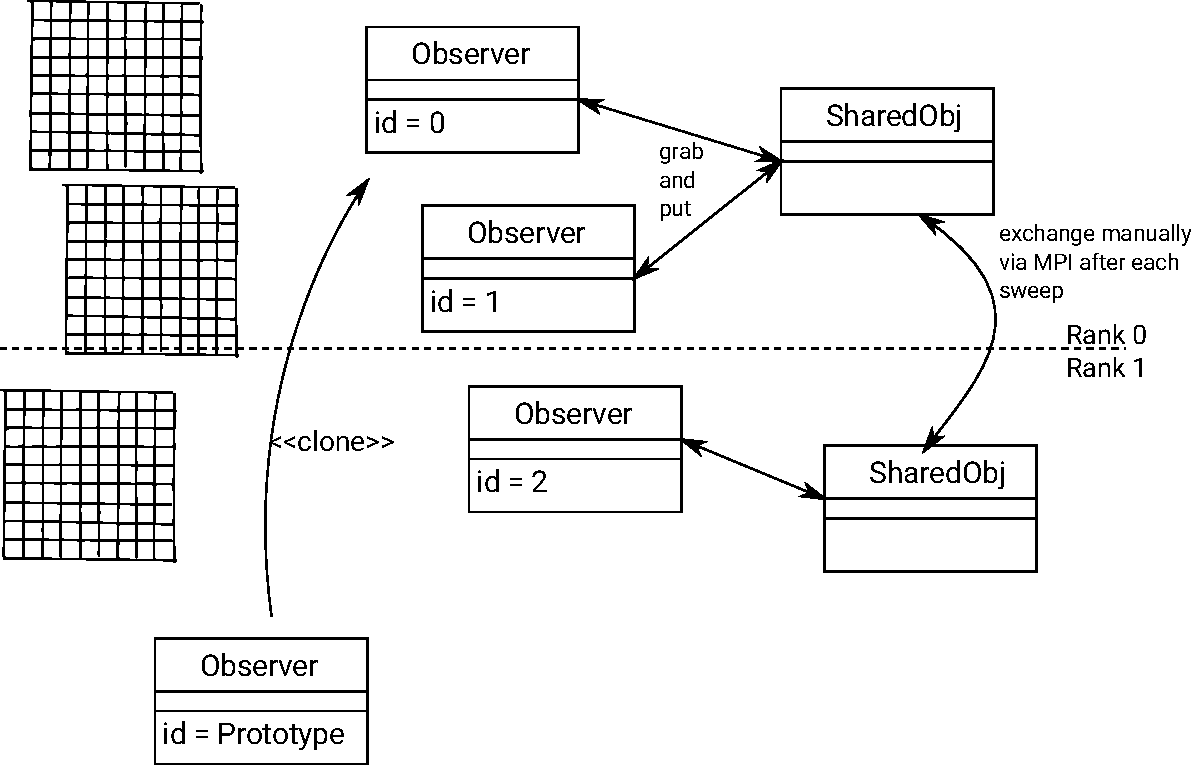
\includegraphics[width=0.75\textwidth]{37_synchronisation/synchronisation-01.pdf}
\end{center}


Here are some pros and cons of this solution:
\begin{itemize}
  \item[+] It is very simple to program;
  \item[+] You have explicit control over when data is reduced from threads into
  the rank-global shared object, and when the individual ranks actually reduce
  their data globally.
  \item[+] You don't have to care how observer clones see a global data
  representation. They always work against a global variable and thus see a
  consistent state always.
  \item[+] If global information expires after an iteration, you can realise
  this ``forget''-mechanism explicitly within your main. Even though you don't
  know when clones are created or destroyed, you know on the main-loop level per
  rank when all local traversals are done or start up.
  \item[-] If the individual observers reduce data into the shared object
  frequently, you have to synchronise manually and you might run into
  performance/locking issues.
\end{itemize}


\begin{remark}
 \ExaHyPE's solvers realise this pattern.
 All the flux functions and Riemann solvers do not exchange data with each
 other---besides the global time step size if we have adaptive time
 stepping---so this seems to be a 
\end{remark}



\subsection*{Global overview file}

Assume each observer writes its own data or file, i.e.~when we clone an observer
(or wen we call its \texttt{beginTraversal}; either option works), we set up all
variables locally.
No race conditions can occur.
When we close the observer, we open a global file in append mode and add a link
to our own data dump.


\begin{center}
 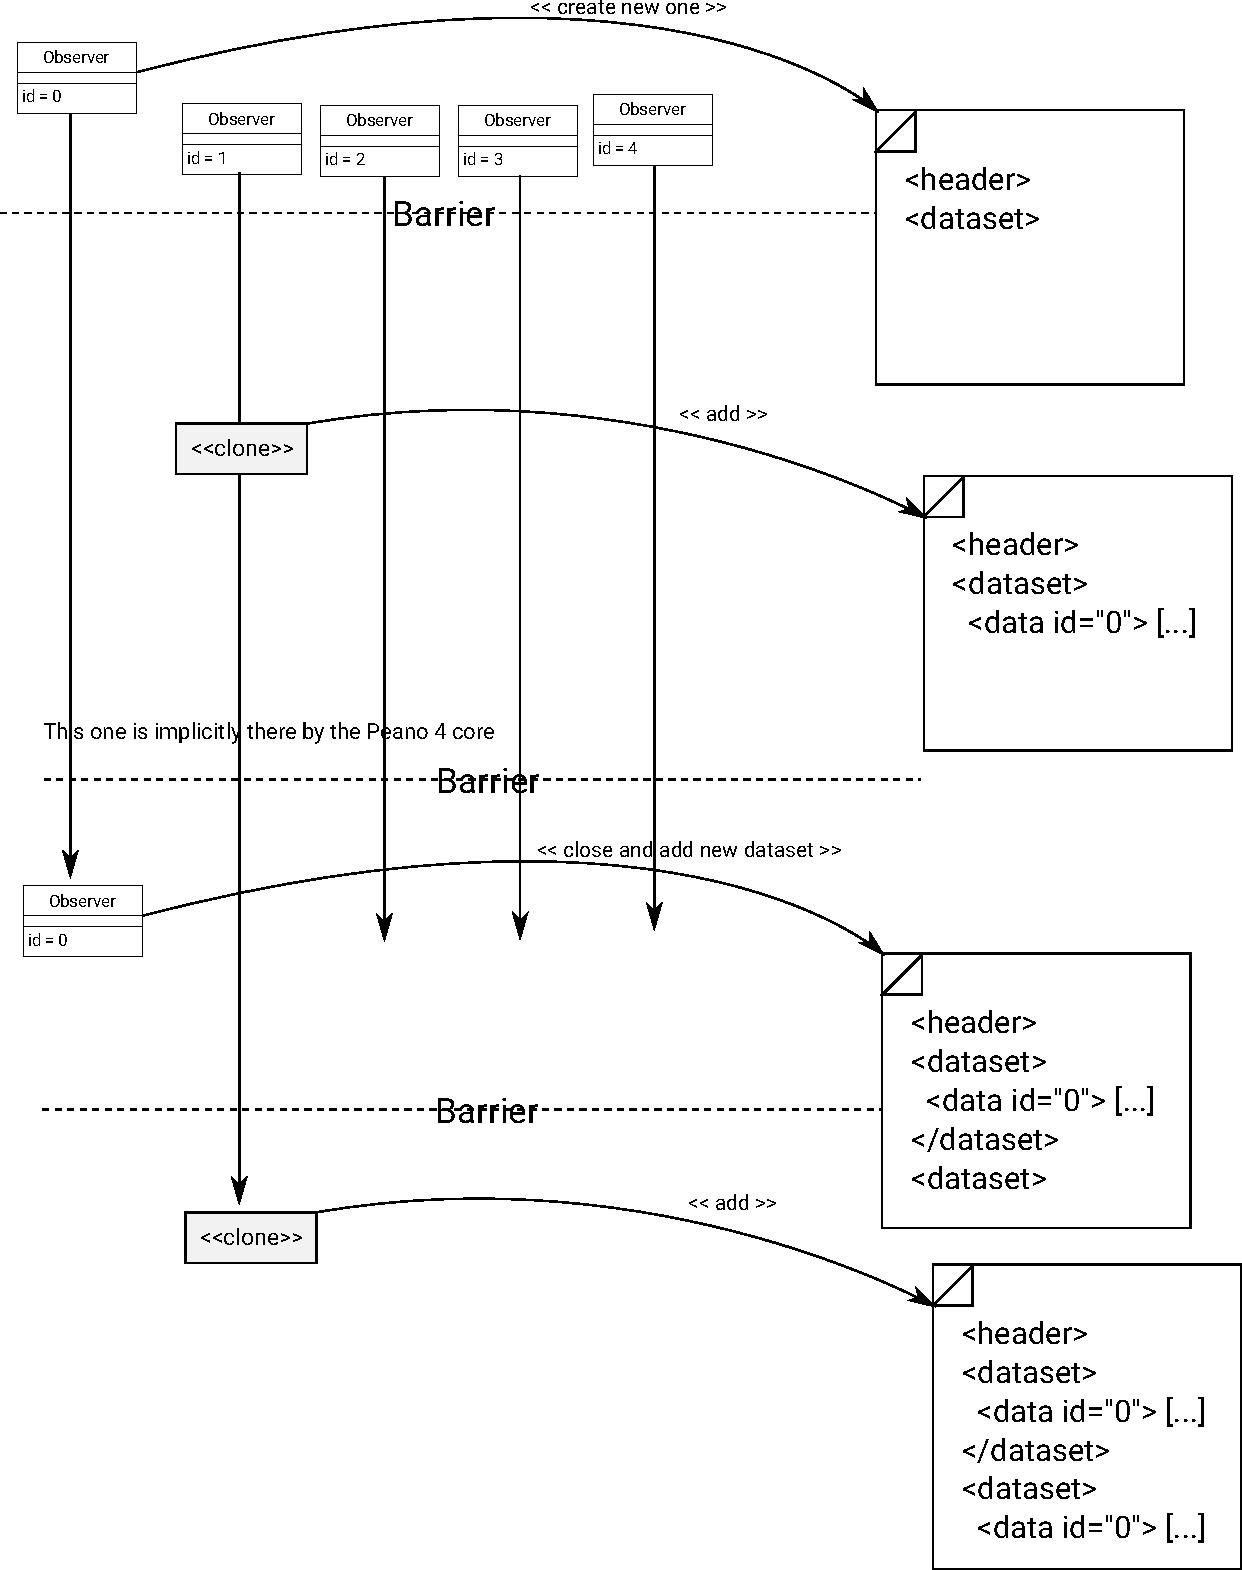
\includegraphics[width=0.75\textwidth]{37_synchronisation/synchronisation-02.pdf}
\end{center}



If we follow this pattern, we get a big blurb of a meta (overview) file and if
we run the code multiple times, we get a meta file which grows and grows and
grows.
So it is clear we have to implement two special rules for tree 0 which is the
only tree we know.
I propose to realise this special knowledge within the clone's construction
where we have the tree number as argument directly.


So if an observer is cloned for tree zero for the very first time (use a static
bool within the function), then we know that this is the very first tree
traversal in the whole run where the global spacetree is traversed.
At this point, it doesn't yet exist. Only the global root plus its children are
there.
So we delete the meta file and create a new one.
This means we are all prepared for all the new data.


Every time we create a new clone for tree number 0, we can know that we've just
kicked off a new traversal over our set of spacetrees.
Consequently, we can add a remark into our meta data file that we are now
starting a new set of dumps.


While this scheme so far is straightforward, it introduced a race condition: 
We cannot be sure that subsequent creations of tree number 0 happen before other
trees create their observer for a new grid sweep.
This is, tree 10 and 11 might have written their dump (and consequently
appended their local data file reference to the global meta file) before we even
start to kick off rank 0's dump.


 
Hence, it is important that we add a barrier to such a dump routine and
protect it via a semaphore.
As we don't really know in which order the observers are cloned, and as we have
to assume that clones are created serially, it is not a good idea to have either
of them in the clone's constructor.
Instead, I recommend that you use your observer's
\texttt{beginTraversal} event.
As we know that the observer creation is kind of lockstepped as all ranks
receive the startup call around the same time.
So it is safe to add a barrier before the routine writing to the meta file
(that's the plotter's constructor, e.g.) for all ranks besides 0.
For 0, it is important to place this barrier after the write into the metafile.
This way, the temporal order of accesses to the metafile is fine.
Next, we protect all accesses to the write via an MPI semaphore
(\texttt{tarch::mpi::BooleanSemaphore}).
Actually, there's no need to protect 0. 
For the other trees, a semaphore however is a must.




\begin{remark}
 \Peano's file dumps from the toolbox work this way.
 These are also the building blocks \ExaHyPE\ uses.
\end{remark}


\subsection*{One data copy per observer}

\marginpar{This is not complete yet}

Let each prototype have a prototype implementation of the shared data.
Let each observer have a standard attribute.
When we clone the prototype per rank, we can also clone this attribute.
Each observer now can work against its local copy of the attribute
independently.
The observers are totally independent of each other and we have, by definition,
no races.


Each observer clone has an operation \texttt{endTraversalOnRank} that
is invoked after the travesal.
This is where we have to restrict data globally.
We know that one tree will always exist and that's tree number 0. 
So we make \texttt{endTraversalOnRank} on all other trees reduce their data


\begin{remark}
 Have to continue to write this one. Its not complete yet!
\end{remark}


\begin{remark}
 \Peano's built-in \texttt{TraversalVTKPlotter} works this way. 
 \ExaHyPE's solvers realise this pattern.
\end{remark}






%   
% % 
% %  \newpage
% %  \section{DaStGen primer and the heap}
\label{section:dastgen-and-heap}




So what we might do now is the following. Open the \texttt{Cell.def} and edit it
accordingly. 
Rerun the PDT, recompile, and work.


\begin{code}
Packed-Type: short int;


class myproject::dastgen::Cell {
  discard    parallelise int     myNonPersistentInteger;
  persistent parallelise double  myValue;
  persistent parallelise bool    myBool1;
  persistent parallelise bool    myBool2;
};
\end{code}


% % 
% %  \newpage
% %  \section{Filling the element-wise traversal with life}

% Element-wise traversal.
% Wo liegen welche Daten
% Enumerator
% Wer aggregiert was
% 
% Remark: How to realise degrees of freedom associated to faces or edges
% 




% We could use the repository's operations
% Do it yourself and then compare
% Finale: Vertices zaehlen
% Den Wert von einem double umsetzen




% 
% 
 \part{Extending the Python API}
 \newpage
 \chapter{Introducing a new pre-defined action set}
\label{section:new-action-set}

This chapter discusses how you make an action set (set of event implementations)
of your code available to other projects as a pre-defined action set.
As a result of such a refactoring, others can inject your ideas
straightforwardly into their project.
The name refactoring suggests that I highly recommend that you start from a
working action set that you've written manually and extensively tested.

\section{Prepare classes}

Create a new subclass of \texttt{peano4.solversteps.ActionSet}

\begin{code}
import peano4.solversteps.ActionSet

class MyActionSet(peano4.solversteps.ActionSet):
  def __init__(self):
    pass
\end{code}

\noindent
and ensure that Python finds the class in its path.


\section{Implement new action set}

To implement the new action set, you have to tell Peano what the function bodies
look like.
Before we do so, we instruct the toolkit whether this is an action set that
users should later on edit; 
that is, your new predefined action set serves as blueprint.
Alternatively, your action set can be read-only and users shall not modify it.
In this case, Peano will place it in the observers' directory and always
regenerate it automatically.


The first step hence is to give your action set a clear name (which will also be
used as class name part for the generated file) and to provide this information:


\begin{code}
  def get_action_set_name(self):
    // My default implementation that I use in the toolboxes is this following
    // line. You are however allowed to use your own, bespoke name
    // return __name__.replace(".py", "").replace(".", "_")
    return "MyName"

  def user_should_modify_template(self):
    return False
\end{code}


\noindent
The actual events are generated through the operation bodies.
All these bodies are queries through one operation. 
The query's arguments clarifies which operation body is requested

\begin{code}
  def get_body_of_operation(self,operation_name):
    # An examples where we only do something for :
    if operation_name == peano4.solversteps.ActionSet.OPERATION_CREATE_CELL:
      return "mycell.add(...)\n"
    return "// Nothing to implement\n"
\end{code}

\noindent
and its values are those constants in \texttt{Mapping} which start with
\texttt{OPERATION\_}.


There are further routines to control the refinement et al.
These routines are self explaining if you study the base class/interface.


More interesting is the question how to make the actual method bodies use grid
information.
For this, the canonical way is that you extend the constructor such that an
object of your action set always ``knows'' which data they work on. 
The interfaces of all action sets are always the same, so it should be
straightforward to make your generated method bodies use the grid data once the
constructor is told what they are.


\section{Use your new action set}

To use the action set, you create your algorithmic steps.
Once created, you also create and instance of your action set and you add it to the
step with \texttt{add\_action\_set}.
The order in which action sets are added is important.
See \texttt{add\_action\_set}'s documentation of information on this.



\section{Conventions}

By default, the Peano toolkit equips each action set with a couple of
features/attributes:

\begin{itemize}
  \item Every action set has a static attribute \texttt{\_log} which is an instance
  of \texttt{tarch::logging::Log}. That is, you can use Peano's logging commands
  straightaway.
\end{itemize}


 
% 
%  \chapter{Applications}
%   \label{chapter:application}
% 
%   \section{The heat equation with an explicit Euler}


\chapterDescription
  {
    60 minutes.
  }
  {
    Chapter \ref{chapter:quickstart}.
  }

In this section, we sketch how to realise a heat equation solver for
\[
  \partial _t u - \nabla (\epsilon \nabla) u = 0
\]
that is based
upon an explicit Euler.
It uses the spacetree as computational grid.


\subsection{Preparation}

We create an empty project with the PDT (\texttt{--create-project myproject
myproject}) and first adopt our cell and vertex data structure such that each
cell holds an $\epsilon$ value and each vertex holds the current and previous
solution.

\begin{code}
Packed-Type: short int;
class myproject::dastgen::Vertex {
  parallelise persistent double  u;
  discard                double  oldU;
};
\end{code}


\begin{code}
Packed-Type: short int;
class myproject::dastgen::Cell {
  persistent double epsilon;
};
\end{code}


\noindent
Furthermore, we make the code's state hold the solver's time step size. We will
write the code such that it works in 2d and 3d. All the pictures are done for a
3d setup. To run with other dimensions, you have to adopt your makefile
accordingly.


\begin{code}
Packed-Type: short int;
class myproject::dastgen::State { 
  persistent parallelise double dt;
};
\end{code}


\noindent
We do not use any sophisticated plotting routines and thus rely in some plotters
that are available out-of-the-box for Peano.
We also require only two mappings: one for the setup, one for the time stepping. 
Depending on our personal choices, we combine them with plotting features or
not\footnote{There is a known issue with the coding standards in Peano/PDT
which can be avoided a priori if all read and write attributes start with an
uppercase---even though they might be defined with lowercase in the def file.}.

\begin{code}
omponent: ExplicitEulerForHeatEquation
namespace: ::myproject
vertex:
  dastgen-file: Vertex.def
  read scalar(double): U
  read scalar(double): OldU
  write scalar(double): U
cell:
  dastgen-file: Cell.def
state:
  dastgen-file: State.def
event-mapping:
  name: CreateGrid
event-mapping:
  name: TimeStep
adapter:
  name: CreateGrid
  merge-with-user-defined-mapping: CreateGrid
adapter:
  name: TimeStep
  merge-with-user-defined-mapping: TimeStep
adapter:
  name: CreateGridAndPlot
  merge-with-user-defined-mapping: CreateGrid
  merge-with-predefined-mapping: VTKPlotCellValue(epsilon,getEpsilon,eps)
  merge-with-predefined-mapping: VTKPlotVertexValue(initialSetup,getU,u)
adapter:
  name: TimeStepAndPlot
  merge-with-user-defined-mapping: TimeStep
  merge-with-predefined-mapping: VTKPlotVertexValue(result,getU,u)
\end{code}

\noindent
To translate this file, you need the corresponding predefined mappings that are 
held in the repository or on the webpage.
To find out what the arguments of the predefined mappings mean, please have a 
look into the corresponding template header files.
We note that we write out epsilon only throughout the setup phase. 
It does not make sense to plot each each iteration, as this material parameter
does not change in time.
We furthermore note that we add some \texttt{read} and \texttt{write}
statements.
They make the PDT generate helper methods that allow us within each cell to
access all $u$ values of a cell as one vector.



\subsection{Making the plotter work}

This code so far does not compile. It complains with

\begin{code}
> make -f myproject/makefile
--- This is Peano 3 ---
g++ -DDim3 [...] -c myproject/adapters/CreateGridAndPlot2VTKPlotCellValue_0.cpp -o \
myproject/adapters/CreateGridAndPlot2VTKPlotCellValue_0.o 
[...]  In member function ‘void [...]::CreateGridAndPlot2VTKPlotCellValue_0::enterCell([...])’:
[...] error: ‘class myproject::Cell’ has no member named ‘getEpsilon’
     _cellValueWriter->plotCell(cellIndex,fineGridCell.getEpsilon() );
                                                       ^
make: *** [myproject/adapters/CreateGridAndPlot2VTKPlotCellValue_0.o] Error 1
\end{code}

\noindent
This is correct. 
We have told the predefined mapping that there would be an opteration
\texttt{getEpsilon} to print cell data, but we have not provided one yet.
A similar reasoning holds for the plotting of the actual solution.
Therefore, we add 

\begin{code}
void myproject::Cell::init() {
  _cellData.setEpsilon( 1.0 + static_cast<double>(rand() % 100)/100.0 );
}

double myproject::Cell::getEpsilon() const {
  return _cellData.getEpsilon();
}
\end{code}

\noindent
This snippet also allows us to initialise a cell with a random value from
$(1,2)$.


\begin{remark}
An initialisation of the cell's $\epsilon$ in the default constructor does not
work because of the flyweight pattern (see next remark). Instead, we have to
provide an explicit initialisation routine, and we have to call this routine
within the mapping's \texttt{createCell} event.
\end{remark}

\noindent
We reiterate our code extension for the vertex,

\begin{code}
double myproject::Vertex::getU() const {
  return _vertexData.getU();
}
\end{code}

\noindent
Finally, we plug into \texttt{CreateGrid}'s \texttt{createInnerVertex} and
\texttt{createBoundaryVertex} and add some refinement statements:

\begin{code}
void myproject::mappings::CreateGrid::createInnerVertex(...) {
 if (coarseGridVerticesEnumerator.getLevel()<3) {
  fineGridVertex.refine();
 }
} 
 
void myproject::mappings::CreateGrid::createBoundaryVertex(...) {
 if (coarseGridVerticesEnumerator.getLevel()<3) {
  fineGridVertex.refine();
 }
} 
 
void myproject::mappings::CreateGrid::createCell(...) {
 logTraceInWith4Arguments( "createCell(...)", fineGridCell, ... );

 fineGridCell.init();

 logTraceOutWith1Argument( "createCell(...)", fineGridCell );
}
  
\end{code}

As soon as this first plot is available, as add a time stepping loop in the
\texttt{runners::Runner}:

\begin{code}
int myproject::runners::Runner::runAsMaster(myproject::repositories::Repository& repository) {
  peano::utils::UserInterface userInterface;
  userInterface.writeHeader();

  repository.switchToCreateGridAndPlot();
  repository.iterate();
  
  repository.getState().setTimeStepSize( 0.5e-7 );
  for (int i=0; i<10000; i++) {
    if (i%100==0) {
      repository.switchToTimeStepAndPlot();
    }
    else {
     repository.switchToTimeStep();
    }
    repository.iterate();
  }
 
  repository.logIterationStatistics();
  repository.terminate();

  return 0;
}
\end{code}

\noindent
The implementation of the \texttt{State}'s \texttt{void setTimeStepSize(double
dt)} operation is left to the reader. 
Please add the corresponding \texttt{double getTimeStepSize() const}, too.

\begin{center}
  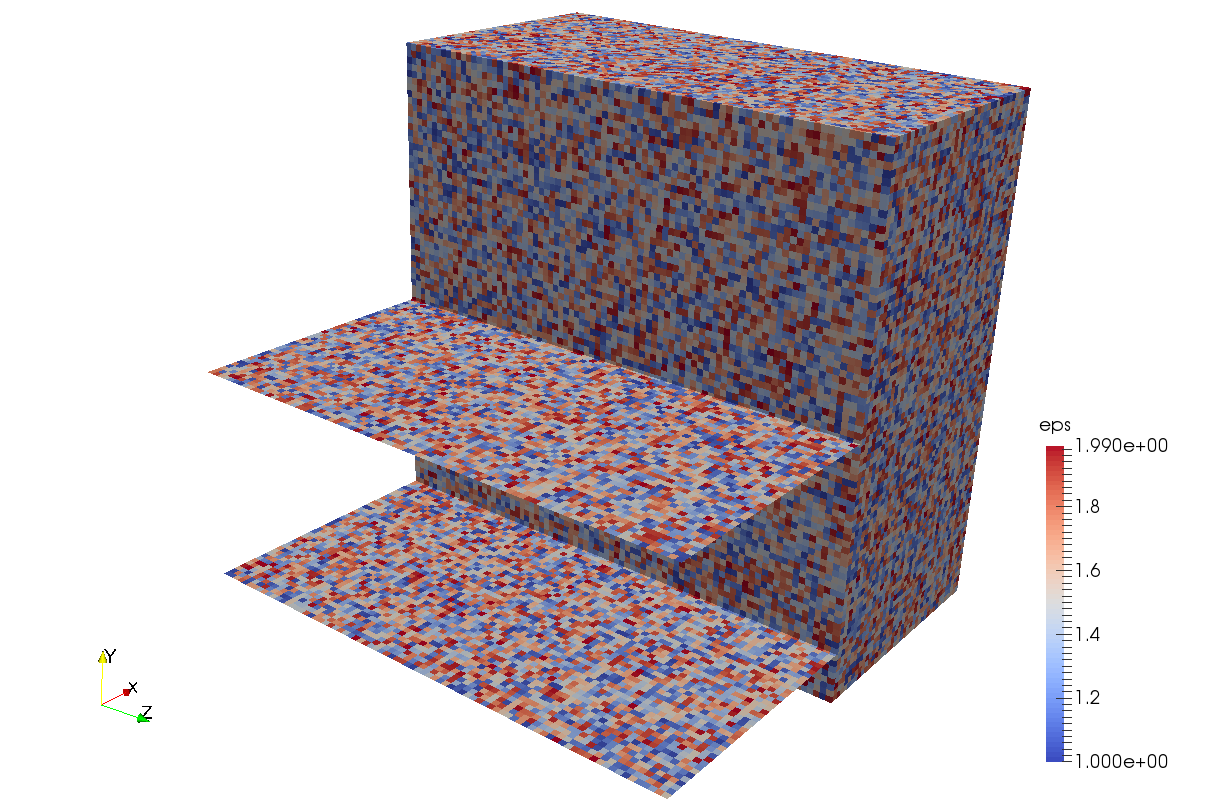
\includegraphics[width=0.7\textwidth]{41_heat-equation/epsilon.png}
\end{center}



\begin{remark}
  It is a `original' decision to model states, vertices and cells as classes
  that actually aggregate their data objects (attribute \texttt{\_stateData},
  \texttt{\_vertexData} or \texttt{\_cellData}, respectively).
  The reason for this is two-fold:
  On the one hand, this allows us to separate user-defined code (the
  aggregating class) from the data model generated by DaStGen. The latter also
  comprises complex technical details such as the MPI data types or bit
  compression. If application-specific code is rewritten, the data model is not
  affected and the other way round. On the other hand, the pattern allows us to
  apply the flyweight pattern. A vertex object is not actually stored and loaded
  from input data. It exists only a few time in total, and in each step its
  change is exchanged underneath by the traversal.
\end{remark}




\subsection{A stencil code}

In this example, we stick to a finite differences formulation and
vertex-centred unknown assignment to do the time stepping.
Our strategy (within the mapping) is simple:
\begin{enumerate}
  \item In \texttt{beginIteration}, we grab the time step size from the state.
  This way, the user might alter the time step size in the outer control loop
  (adaptive time stepping).
  The mapping then always works with the right parameter.
  \item In \texttt{touchVertexFirstTime}, we take the current solution and back
  it up in the vertex's property \texttt{\_oldU}. This property is marked as
  discard, i.e.~the additional helper variable per vertex is not held in-between
  two iterations (actually it is only held for a small number of vertices that
  are still in use). 
  \item In \texttt{enterCell}, we element-wisely accumulate the new solution in
  the vertices.
\end{enumerate}

\begin{code}
class myproject::mappings::TimeStep {
 private:
  /**
   * Logging device for the trace macros.
   */
  static tarch::logging::Log  _log;
    
  double _timeStepSize;
  ...
};


void myproject::mappings::TimeStep::beginIteration(
  myproject::State&  solverState
) {
  logTraceInWith1Argument( "beginIteration(State)", solverState );

  _timeStepSize = solverState.getTimeStepSize();

  logTraceOutWith1Argument( "beginIteration(State)", solverState);
}
\end{code}

\noindent
We reiterate that the state is not available to a mapping by default. If you
need the state (or one of its properties), you explicitly have to grab this data
in \texttt{beginIteration}. As an alternative to the double above, it also would
be possible to copy the whole state. If you want to modify the solver's state,
you have to alter it in \texttt{endIteration}. As Peano requires the user to
explicitly move state data around when required, we ensure that the data remains
consistent in the parallel code variants.

\begin{code}
void myproject::mappings::TimeStep::touchVertexFirstTime(...) {
 ...  
 fineGridVertex.copyCurrentSolutionIntoOldSolution();
 ...  
}

void myproject::Vertex::copyCurrentSolutionIntoOldSolution() {
  _vertexData.setOldU( _vertexData.getU() );
}
\end{code}

\noindent
The interesting stuff happens in the mapping's \texttt{enterCell}, 
where we first of all take all $2^d$ vertices and write their old solution into
one double vector. 
For this, there's a predefined operation in \texttt{VertexOperations} as we have
asked the PDE that we read the scalar.
This $2^d$ vector then is multiplied with the local assembly matrix subject of
an $\epsilon$ scaling.
The result finally is added to the new value.
Again, we us the generated read and write methods.

\begin{code}
#include "myproject/VertexOperations.h"
#include "tarch/la/Matrix.h"

void myproject::mappings::TimeStep::enterCell(...) {
  logTraceInWith4Arguments( "enterCell(...)", fineGridCell, ... );

  tarch::la::Matrix<TWO_POWER_D,TWO_POWER_D,double> A;

  A =  6.0/8.0, -1.0/4.0, -1.0/4.0,      0.0, -1.0/4.0,      0.0,      0.0,      0.0,
      -1.0/4.0,  6.0/8.0,      0.0, -1.0/4.0,      0.0, -1.0/4.0,      0.0,      0.0,
      -1.0/4.0,      0.0,  6.0/8.0, -1.0/4.0,      0.0,      0.0, -1.0/4.0,      0.0,
           0.0, -1.0/4.0, -1.0/4.0,  6.0/8.0,      0.0,      0.0,      0.0, -1.0/4.0,
      -1.0/4.0,      0.0,      0.0,      0.0,  6.0/8.0, -1.0/4.0, -1.0/4.0,      0.0,
           0.0, -1.0/4.0,      0.0,      0.0, -1.0/4.0,  6.0/8.0,      0.0, -1.0/4.0,
           0.0,      0.0, -1.0/4.0,      0.0, -1.0/4.0,      0.0,  6.0/8.0, -1.0/4.0,
           0.0,      0.0,      0.0, -1.0/4.0,      0.0, -1.0/4.0, -1.0/4.0,  6.0/8.0;

  tarch::la::Vector<TWO_POWER_D,double> uOld = 
    VertexOperations::readOldU(fineGridVerticesEnumerator,fineGridVertices);

  const double h = fineGridVerticesEnumerator.getCellSize()(0);

  tarch::la::Vector<TWO_POWER_D,double> uUpdate = 
    - _timeStepSize * fineGridCell.getEpsilon() * A * uOld / h / h  ;

  VertexOperations::writeU(
    fineGridVerticesEnumerator,fineGridVertices,
    VertexOperations::readU(fineGridVerticesEnumerator,fineGridVertices) + uUpdate
  );

  logTraceOutWith1Argument( "enterCell(...)", fineGridCell );
}
\end{code}

\noindent
In this example, I wrote down the local assembly matrix for $d=3$ explicitly.
If you want to support other dimensions, you have to adopt this part
accordingly.

We use Peano's linear algebra routines here.
They are held in the \texttt{tarch} component, and provide all basic
functionality we typically need.
Obviously, it might make sense to switch to other linear algebra packages
(BLAS, e.g.) for more demanding setups.

For a better understanding, it might make sense to have a look into
\texttt{readOldU}.
We note that \texttt{fineGridVertices} is a pointer to an array of vertices, but
the layout of the vertices within this array remains open.
Therefore, Peano hands over an enumerator object. 
The enumerator object has a functor to allow us to select the right vertices.
\texttt{fineGridVertices[ fineGridVerticesEnumerator(0) ]} for example returns
the bottom left vertex of the cell.
See the enumerator's documentation in the header for detailed information.
The read and write that are generated by the PDT run through the vertices and
collect the \texttt{u} or \texttt{oldU} value, respectively, in one vector.
They are scatter/gather operations.
Some codes might prefer not to rely on the temporary vectors and instead work
with the data associated to the vertices directly.
Both options are fine, both options might have different performance
characteristics.

 
Obviously, the above code is not very elaborate. 
The stiffness matrix is set up multiple times.
The most basic optimisation would be to make the matrix an attribute of the
mapping and to initialise it only once.

\begin{remark}
  On the Peano webpage and in the repository, you find a \texttt{matrixfree}
  toolbox. It contains all kind of primitive helper operations that allow you to
  work with stencil codes. It is not as powerful as a real stencil compiler or 
  other matrix-free/PDE toolboxes, but it a small suite to build up at least the
  simpler PDE operators from a finite element/tensor-product formalism and it
  also provides operations fitted to PDT's generated read and write routines. 
The toolbox also provides helper functions that decompose stencils in element-wise
assembly matrices as the one above.
\end{remark}


\noindent
Obviously, our code does not do anything as we do not set any nonzero boundary
conditions. 
Lets do this upon a vertex's first use. 
As we have specified a read, the PDT provides write operations that break up the
object encapsulation.
We make use of this now:

\begin{code}
void myproject::mappings::TimeStep::touchVertexFirstTime(...) {
  ...
  if (fineGridVertex.isBoundary() && fineGridX(0)<1e-8) {
    VertexOperations::writeU( fineGridVertex, 1.0 );
  }
  else if (fineGridVertex.isBoundary()) {
    VertexOperations::writeU( fineGridVertex, 0.0 );
  }
  ...
}
\end{code}

\begin{remark}
In this example, we do not ensure that we do not update boundary vertices.
Indeed, we update them, but in the subsequent traversal we overwrite them again
with the prescribed Dirichlet values (code snippet above). Most codes rather add
an additional if statement checking \texttt{fineGridVertex.isBoundary()}.
\end{remark}

\begin{center}
  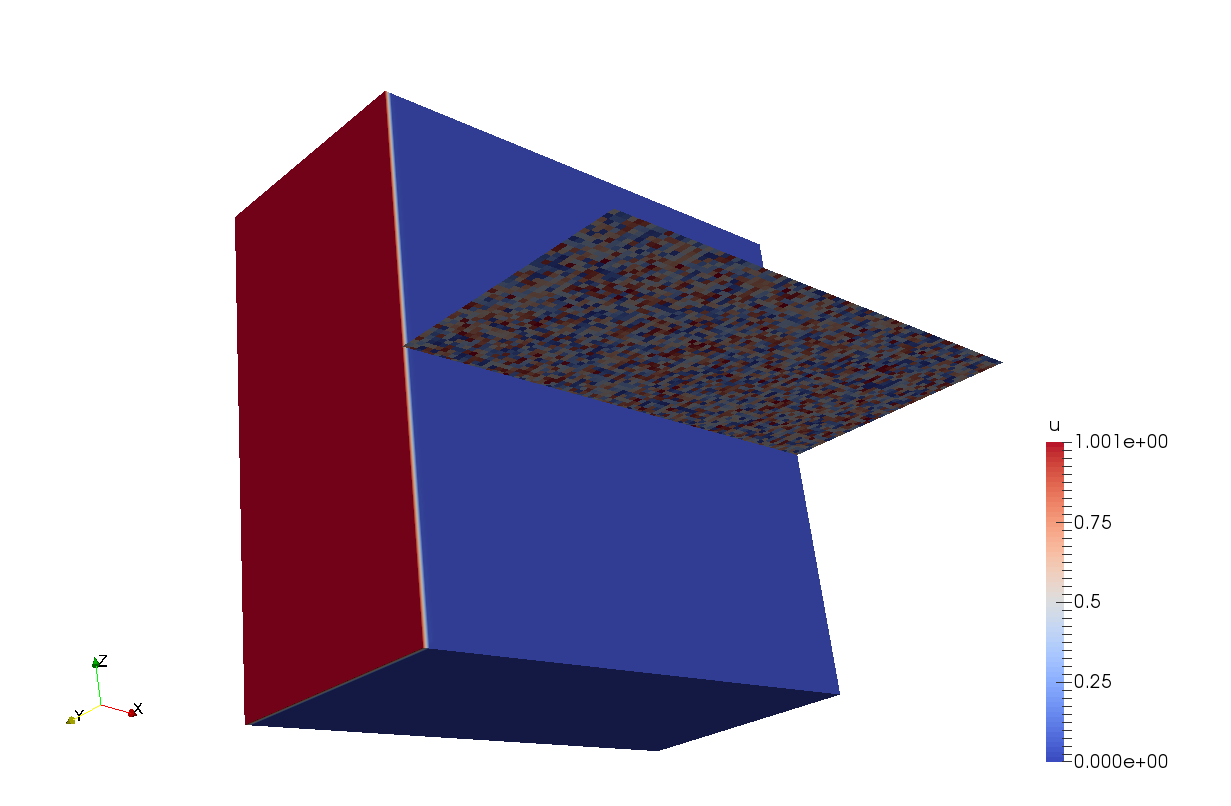
\includegraphics[width=0.45\textwidth]{41_heat-equation/solution00.png}
  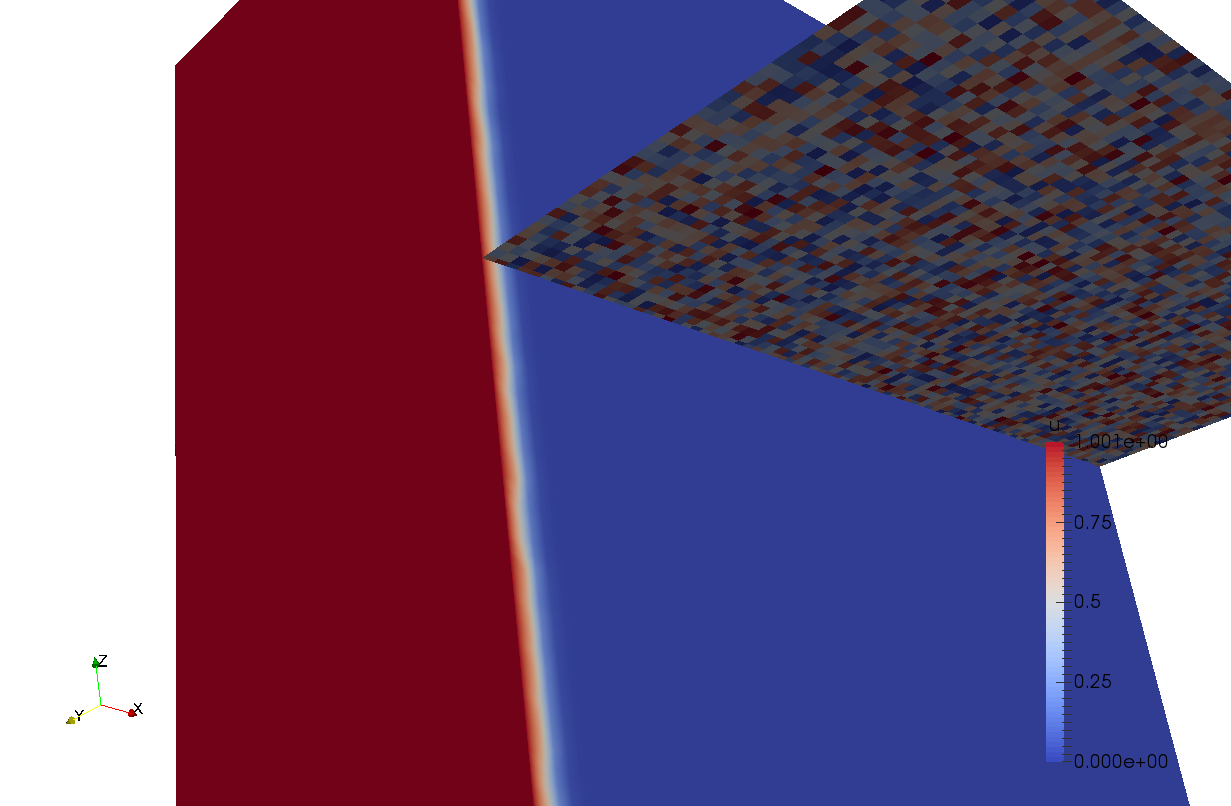
\includegraphics[width=0.45\textwidth]{41_heat-equation/solution01.png}
  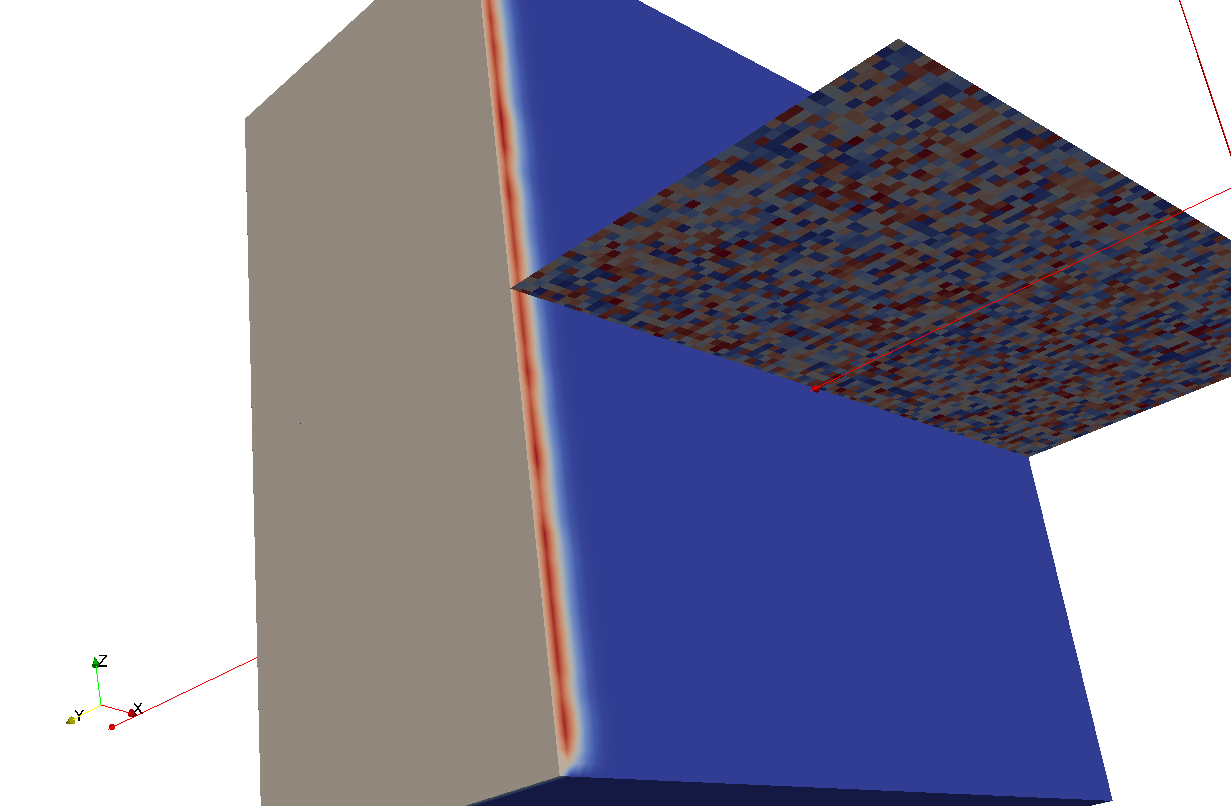
\includegraphics[width=0.45\textwidth]{41_heat-equation/solution02.png}
  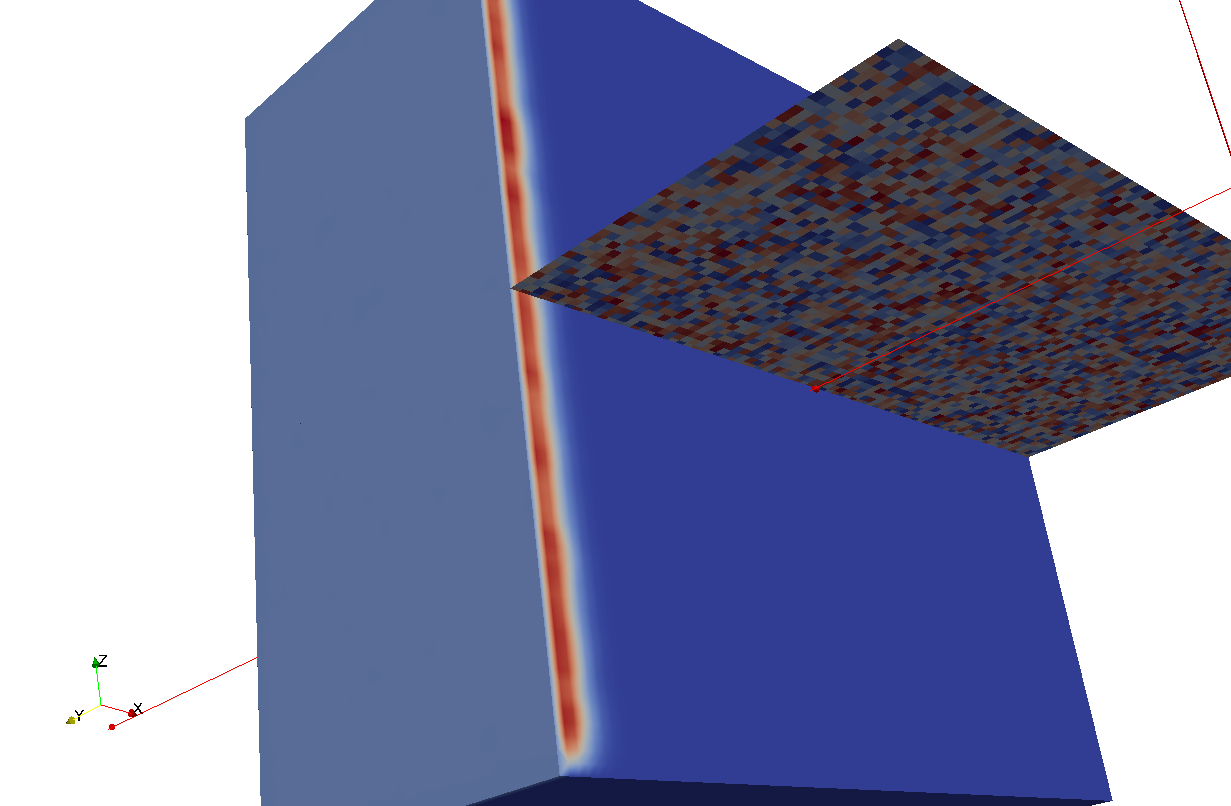
\includegraphics[width=0.45\textwidth]{41_heat-equation/solution03.png}
\end{center}


All figures cut through the domain in the middle and use an orthogonal slice to
visualise the permeability $\epsilon$.
Top, left: We start from a zero condition where only the face at $x=0$ is set to
$1$.
Top, right: Very slowly, the temperature propagates through the domain. As
$\epsilon $ is fuzzy, the propagation profile does not exhibit symmetry but is
ragged as well.
Bottom: The temperature propagates further into the medium.


\subsection{Multiscale data representation}

We continue the solver development with a technical extension that proofs to be
of great value.
Rather than working on the actual fine grid, i.e.~our compute grid, we inject
the finest solutions to the coarser grids all the time:
whenever a vertex coincides with a vertex on a coarser level, we take its value
and copy it to the coarser grid.
To realise this injection, we typically propose to introduce a new mapping in
the specification, and to realise the injection in this new mapping---it has
nothing to do directly with the solver, so the separation of mappings reflects a
separation of concerns.

\begin{code}
...
event-mapping:
  name: Inject
...
adapter:
  name: TimeStep
  merge-with-user-defined-mapping: TimeStep
  merge-with-user-defined-mapping: Inject
...
adapter:
  name: TimeStepAndPlot
  merge-with-user-defined-mapping: TimeStep
  merge-with-user-defined-mapping: Inject
  merge-with-predefined-mapping: VTKPlotVertexValue(result,getU,u)
\end{code}


\noindent
As a result, we have a multiscale representation of the solution on each
individual grid level.
It is (almost) for free, as Peano's vertices are unique due to their combination
of level and spatial position, i.e.~these coarse vertices do exist anyway.

\begin{code}
void myproject::Vertex::inject(const Vertex& fromVertex) {
  _vertexData.setU( fromVertex._vertexData.getU() );
}

void myproject::mappings::Inject::touchVertexLastTime(...) {
 logTraceInWith6Arguments( "touchVertexLastTime(...)", fineGridVertex, fineGridX, ... );

 if ( peano::grid::SingleLevelEnumerator::isVertexPositionAlsoACoarseVertexPosition(
  fineGridPositionOfVertex) ) {
  const peano::grid::SingleLevelEnumerator::LocalVertexIntegerIndex coarseGridPosition = 
   peano::grid::SingleLevelEnumerator::getVertexPositionOnCoarserLevel
   (fineGridPositionOfVertex);

  coarseGridVertices[ coarseGridVerticesEnumerator(coarseGridPosition) ].inject(fineGridVertex);
 }

 logTraceOutWith1Argument( "touchVertexLastTime(...)", fineGridVertex );
}
\end{code}

\noindent
In our implementation, we use helper functions of the enumerator classes. 
Alternatively, we could have checked the integer array
\texttt{fineGridPosiitionOfVertex} manually whether all entries are either 0 or
3.


\begin{remark}
Several projects have exploited this multiscale representation for visualisation
and data postprocessing. Whenever data in a reduced accuracy is sufficient (to
create fancy pictures, e.g.), one can directly extract this data from the
corresponding spacetree level rather than using the finest grid representation
and postprocess these data.
\end{remark}

\subsection{Static adaptivity}

An elegant way to realise adaptive solvers is to pick up the concept of FAC/MLAT
from the multigrid community.
The idea is very simple:
\begin{itemize}
  \item We calculate an update of the solution for each and every cell in the
  sapcetree. This includes the refined ones.
  \item We interpolate hanging nodes from the next coarser levels. This can be
  done recursively, i.e.~a 3:1 balancing of the tree is not required. Rippling
  does not happen.
  \item We inject the solution of a fine grid vertex to the coarser levels and
  thus overwrite the impact of the unknown update there. 
\end{itemize}

\begin{center}
 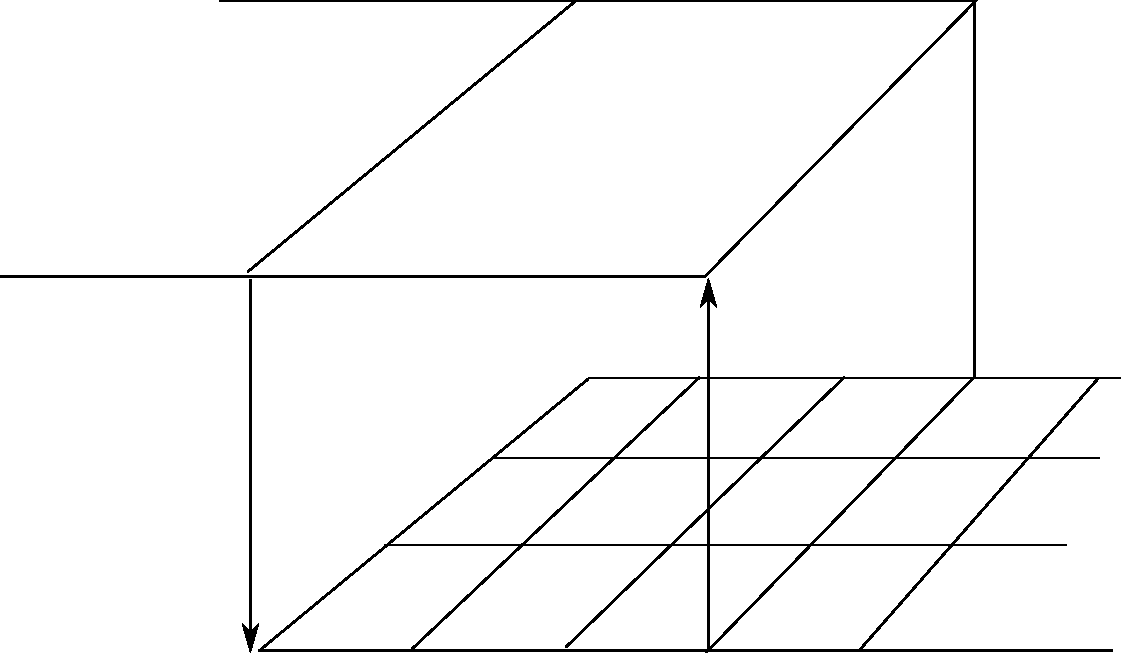
\includegraphics[width=0.34\textwidth]{41_heat-equation/FAC.pdf}
\end{center}


\noindent
One can read such a scheme as an overlapping domain decomposition: 
The coarser levels slightly overlap finer levels. 
Those coarse grid vertices that fall into a fine grid partition are treated as
Dirichlet values (we may update them, but the update then is overwritten
immediately).
Their value is injected from finer grids---an ingredient we already have
realised.
Fine grid problems are handled as Dirichlet problems as well. 
Their boundary points either are real boundary points or hanging nodes.
The value of hanging nodes in turn stems from coarser levels which closes the
coupling of the coarse and fine grid problems.


We propose to introduce---mirroring \texttt{Inject}---a new mapping
\texttt{InterpolateHangingNodes} that solely plugs into the generation of hanging nodes.
This time, we use Peano's $d$-dimensional loops, as well as PDT's generated
write operations that break up the OO encapsulation.

\begin{code}
#include "myproject/VertexOperations.h"
#include "peano/utils/Loop.h"

void myproject::mappings::InterpolateHangingNodes::createHangingVertex(...) {
  logTraceInWith6Arguments( "createHangingVertex(...)", fineGridVertex, fineGridX, ... );

  double interpolatedValue = 0.0;
  dfor2(k)
    double weight = 1.0;
    for (int d=0; d<DIMENSIONS; d++) {
      if (k(d)==0) {
        weight *= 1.0 - (fineGridPositionOfVertex(d))/3.0;
      }
      else {
        weight *= (fineGridPositionOfVertex(d))/3.0;
      }
    }
    interpolatedValue = weight * coarseGridVertices[ coarseGridVerticesEnumerator(k)].getU();
  enddforx

  VertexOperations::writeU( fineGridVertex, interpolatedValue );
  fineGridVertex.copyCurrentSolutionIntoOldSolution();

  logTraceOutWith1Argument( "createHangingVertex(...)", fineGridVertex );
}
\end{code}

\noindent
We reiterate that Peano's \texttt{matrixfree} toolbox provides helpers realising
such typical interpolation tasks.

Finally, we have to setup an adaptive grid. We stick to a static, simple setup
for the time being where the mesh is made very fine along the $x=0$ plane and
reasonably coarse everywhere else.
Please note that you might have to adopt your time step size as well if you
reduce the resolution along the heated up plate.
Furthermore, if you visualise, please note that the default visualiser we used
so far does not know anything about the hanging nodes' interpolation and thus
plots them as zero values. 

\begin{code}
void myproject::mappings::CreateGrid::createInnerVertex(...) {
 if (coarseGridVerticesEnumerator.getLevel()<1) {
  fineGridVertex.refine();
 }
}

void myproject::mappings::CreateGrid::createBoundaryVertex(...) {
 if (coarseGridVerticesEnumerator.getLevel()<3 && fineGridX(0)<1e-8) {
  fineGridVertex.refine();
 }
 else if (coarseGridVerticesEnumerator.getLevel()<1) {
  fineGridVertex.refine();
 }
}
\end{code}


\begin{center}
 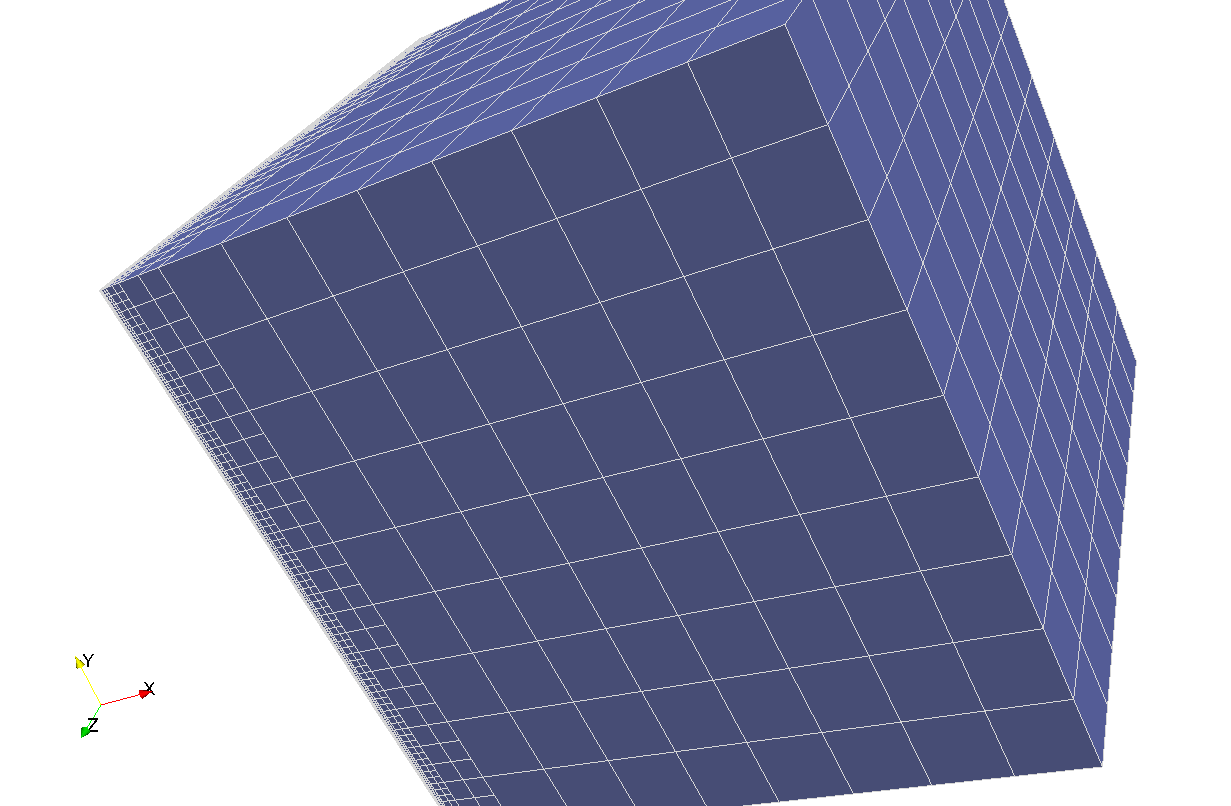
\includegraphics[width=0.45\textwidth]{41_heat-equation/initial-adaptive-grid.png}
 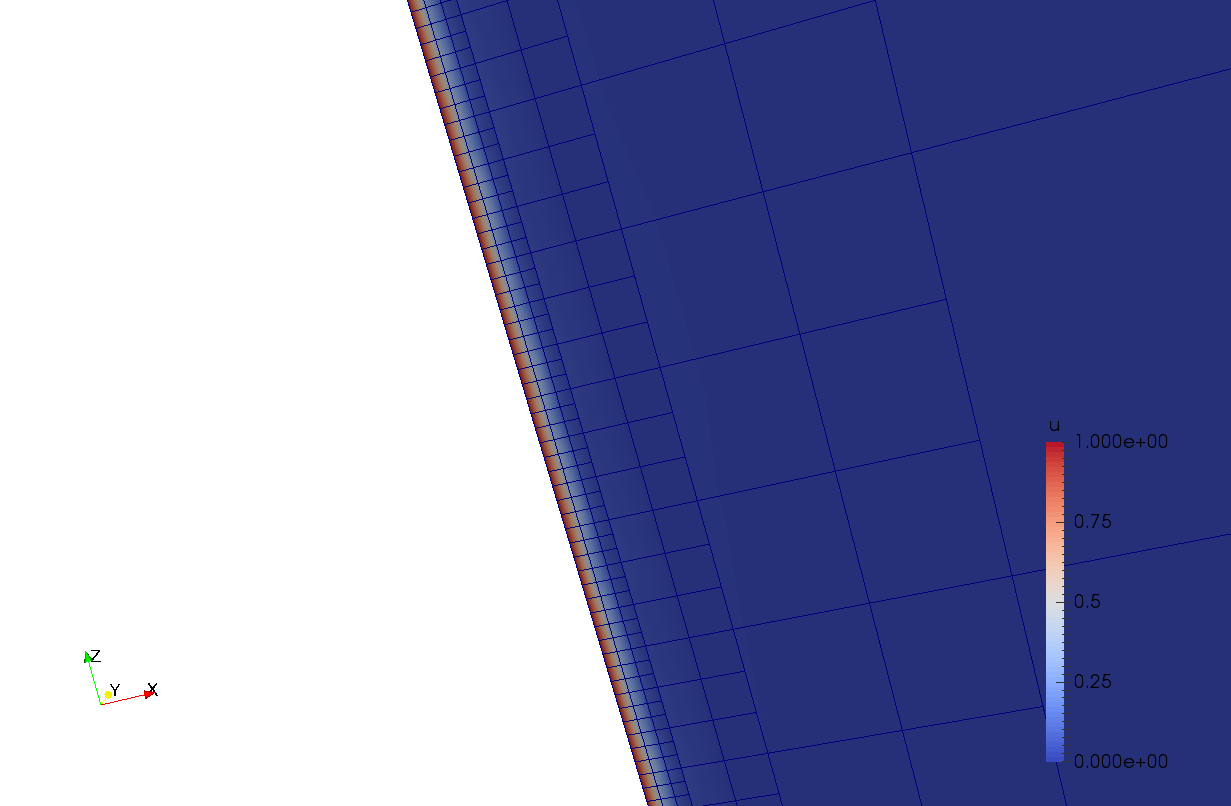
\includegraphics[width=0.45\textwidth]{41_heat-equation/adaptive-grid-21.png}
\end{center}


\noindent
In the present example, it does not matter that some cells compute stencil
evaluations that are never used:
These are the cells where all adjacent vertices are refined.
Due to the injection, the stencil evalution here is not necessary.
As the stencils are very small and cheap to evaluate, this does not make a
difference.
For more complicated setups, it however might make a difference.

Obviously, it is not possible in the present case to use the cells'
\texttt{isRefined()} operation to determine whether a stencil evaluation should
be skipped or not.
Refined cells next to an unrefined one have to be taken into account.
Instead, we have to run over all adjacent vertices of a cell and determine their
refinement state.
Peano realises an or-based refinement---if any vertex adjacent to a cell carries
the refinement bit, the cell is refined---so the required check is an or
combination followed by a negation.
In Peano, there's a class \texttt{peano::grid::aspects::VertexStateAnalysis}.
It is worth to study this class; it offers most of such analysis routines
already and makes the programming of multiscale algorithms more convenient.


\subsection{Dynamic adaptivity}

Given a statically adaptive grid, dynamic adaptivity is (technically) a minor
improvement. 
We realise it in two steps:
\begin{enumerate}
  \item We write the refinement criterion, and 
  \item we ensure that the a posteriori refinement initialises the correct data.
\end{enumerate}

The first step is strongly application dependent. 
A simple criterion that seems to work sufficiently is to assign each vertex a
new (non-persistent) value that holds the average value of the surrounding
vertices. 
If this value differs significantly from the computed value in the point (which
is kind of a smoothness analysis), we refine.
For this, we change the vertex definition
\begin{code}
Packed-Type: short int;


class myproject::dastgen::Vertex {  
  parallelise persistent double  u;
  discard    double  oldU;
  discard    double  averagedU;
};
\end{code}

\noindent
and we also add additional read statements to the specification.
The specification remains more or less unchanged, but we keep all the dynamic
refinement in an additional refinement mapping.

\begin{code}
vertex:
  dastgen-file: Vertex.def
  read scalar(double): U
  read scalar(double): OldU
  read scalar(double): AveragedU
  write scalar(double): U
  write scalar(double): AveragedU
  
...

event-mapping:
  name: RefineDynamically

...

adapter:
  name: TimeStep
  merge-with-user-defined-mapping: TimeStep
  merge-with-user-defined-mapping: Inject
  merge-with-user-defined-mapping: InterpolateHangingNodes
  merge-with-user-defined-mapping: RefineDynamically
\end{code}

\noindent
Before we implement this additional mapping, we create a slightly more appealing
problem setup in create grid:
\begin{code}
void myproject::mappings::CreateGrid::createCell(...) {
  logTraceInWith4Arguments( "createCell(...)", fineGridCell, ... );

  fineGridCell.init( fineGridVerticesEnumerator.getCellCenter() );

  logTraceOutWith1Argument( "createCell(...)", fineGridCell );
}


void myproject::Cell::init(const tarch::la::Vector<DIMENSIONS,double>&  x) {
  _cellData.setEpsilon( x(1) * x(2) + static_cast<double>(rand() % 100)/100.0 );
}
\end{code}

\noindent
Furthermore, we make the start grid one level coarser along the $x=0$ axis 
compared to the previous setup.

Our refinement criterion materialises in a very simple mapping relying on the
simple stencil (here given for two dimensions)
\[
\left[ \begin{array}{ccc}
  0 & 1 & 0 \\
  -1 & 0 & 1 \\
  0 & -1 & 0
\end{array}  \right]
\]
that we apply on the solution.
This stencil determines the derivative in a point.
For a first try, it often yields very reasonable refinement patterns---we
refine where we observe a steep gradient.

\begin{code}
void myproject::mappings::AdaptiveRefinementCriterion::touchVertexFirstTime(...) { 
  logTraceInWith6Arguments( "touchVertexFirstTime(...)", fineGridVertex, ... );

  VertexOperations::writeAveragedU( fineGridVertex, 0.0 );

  logTraceOutWith1Argument( "touchVertexFirstTime(...)", fineGridVertex );
}


void myproject::mappings::AdaptiveRefinementCriterion::enterCell(...) {
  logTraceInWith4Arguments( "enterCell(...)", fineGridCell, ... );

  tarch::la::Matrix<TWO_POWER_D,TWO_POWER_D,double> A;

  A =  0.0,  1.0/4.0,  1.0/4.0,  0.0,  1.0/4.0,  0.0,  0.0,  0.0,
      -1.0/4.0,  0.0,  0.0,  1.0/4.0,  0.0,  1.0/4.0,  0.0,  0.0,
      -1.0/4.0,  0.0,  0.0,  1.0/4.0,  0.0,  0.0,  1.0/4.0,  0.0,
       0.0, -1.0/4.0, -1.0/4.0,  0.0,  0.0,  0.0,  0.0,  1.0/4.0,
      -1.0/4.0,  0.0,  0.0,  0.0,  0.0,  1.0/4.0,  1.0/4.0,  0.0,
       0.0, -1.0/4.0,  0.0,  0.0, -1.0/4.0,  0.0,  0.0,  1.0/4.0,
       0.0,  0.0, -1.0/4.0,  0.0, -1.0/4.0,  0.0,  0.0,  1.0/4.0,
       0.0,  0.0,  0.0, -1.0/4.0,  0.0, -1.0/4.0, -1.0/4.0,  0.0;

  tarch::la::Vector<TWO_POWER_D,double> uOld = 
    VertexOperations::readOldU(fineGridVerticesEnumerator,fineGridVertices);

  const double h       = fineGridVerticesEnumerator.getCellSize()(0);
  const double scaling = 1.0/h;
  tarch::la::Vector<TWO_POWER_D,double> averageUpdate = scaling * A * uOld;

  VertexOperations::writeAveragedU(
    fineGridVerticesEnumerator,fineGridVertices,
    VertexOperations::readAveragedU(fineGridVerticesEnumerator,fineGridVertices) 
    + averageUpdate
  );
 
  logTraceOutWith1Argument( "enterCell(...)", fineGridCell );
}


void myproject::mappings::AdaptiveRefinementCriterion::touchVertexLastTime(...) { 
  logTraceInWith6Arguments( "touchVertexLastTime(...)", fineGridVertex, fineGridX, ... );

  if (coarseGridVerticesEnumerator.getLevel()<6) {
    fineGridVertex.evaluateRefinementCiterion();
  }

  logTraceOutWith1Argument( "touchVertexLastTime(...)", fineGridVertex );
}

\end{code}


\noindent
The magic final operation is kept very simple in this guide book:

\begin{code}
void myproject::Vertex::evaluateRefinementCiterion() {
 if (
  getRefinementControl()==Records::Unrefined
  &&
  std::abs( _vertexData.getAveragedU() )>1.0
 ) {
   refine();
 }
}
\end{code}

\begin{remark}
Almost all sophisticated refinement criteria are based upon a marker concept
such that only a given ratio of the cells are refined per step. 
Such markers are non-trivial to implement as they require global sorting.
It is thus convenient to use some binning approach.
The \texttt{matrixfree} toolbox of Peano has a reference implementation that
also works in an MPI environment.
\end{remark}

For the second step, we have to ensure that all newly created cells and vertices
are intialised correctly.
For the cells, we might simply merge the \texttt{CreateGrid} mapping into our
time stepping adapter.
For the vertices, we have to plug into \texttt{createInnerVertex} where we
initialse the vertex with the interpolated value of its coarse grid parents.
Again, Peano offers toolboxes with routines that do so. 
However, you may also simply reprogram it using the dimension-specific for-loops
of \texttt{Loop.h}.
The routines are then very similar to the interpolation for hanging nodes.
In this example, we do not reuse \texttt{CreateGrid}, but implement everything
within the adaptivity criterion's mapping.

\begin{code}
void myproject::mappings::AdaptiveRefinementCriterion::createCell( ... ) {
  logTraceInWith4Arguments( "createCell(...)", fineGridCell, ... );

  fineGridCell.init( fineGridVerticesEnumerator.getCellCenter() );

  logTraceOutWith1Argument( "createCell(...)", fineGridCell );
}


void myproject::mappings::AdaptiveRefinementCriterion::createInnerVertex( ... ) {
  logTraceInWith6Arguments( "createInnerVertex(...)", fineGridVertex, fineGridX, fineGridH, ... );

  double interpolatedValue = 0.0;
  dfor2(k)
    double weight = 1.0;
    for (int d=0; d<DIMENSIONS; d++) {
      if (k(d)==0) {
        weight *= 1.0 - (fineGridPositionOfVertex(d))/3.0;
      }
      else {
        weight *= (fineGridPositionOfVertex(d))/3.0;
      }
    }
    interpolatedValue = weight * coarseGridVertices[ coarseGridVerticesEnumerator(k)].getU();
  enddforx

  VertexOperations::writeU( fineGridVertex, interpolatedValue );
  fineGridVertex.copyCurrentSolutionIntoOldSolution();

  logTraceOutWith1Argument( "createInnerVertex(...)", fineGridVertex );
}
\end{code}

\noindent
We finally modifiy our runner in two ways:
\begin{enumerate}
  \item We make the runner also plot if the grid changes in a particular time
  step, and
  \item we ensure that the time step size adopts to the grid structure, i.e.~we
  implement adaptive time stepping.
\end{enumerate}

\begin{code}
int myproject::runners::Runner::runAsMaster(myproject::repositories::Repository& repository) {
 peano::utils::UserInterface userInterface;
 userInterface.writeHeader();

 repository.switchToCreateGridAndPlot();
 repository.iterate();
  
 const double initialDt = 1e-4;
 repository.getState().setTimeStepSize( initialDt );
 for (int i=0; i<10000; i++) {
   if (i%100==0 || !repository.getState().isGridStationary()) {
     repository.switchToTimeStepAndPlot();
   }
   else {
    repository.switchToTimeStep();
   }
   repository.iterate();
   double dt = initialDt * repository.getState().getMinimumMeshWidth() 
             * repository.getState().getMinimumMeshWidth();
   repository.getState().setTimeStepSize( dt );
   logInfo( 
    "runAsMaster(...)", 
    "time step " << i << ": dt=" << dt << ", h_min=" <<
    repository.getState().getMinimumMeshWidth() ); 
 }
 
 repository.logIterationStatistics();
 repository.terminate();

 return 0;
}
\end{code}


\noindent
The screenshots below illustrate how the grid evolves in the first four time
steps of the simulation:
\begin{center}
  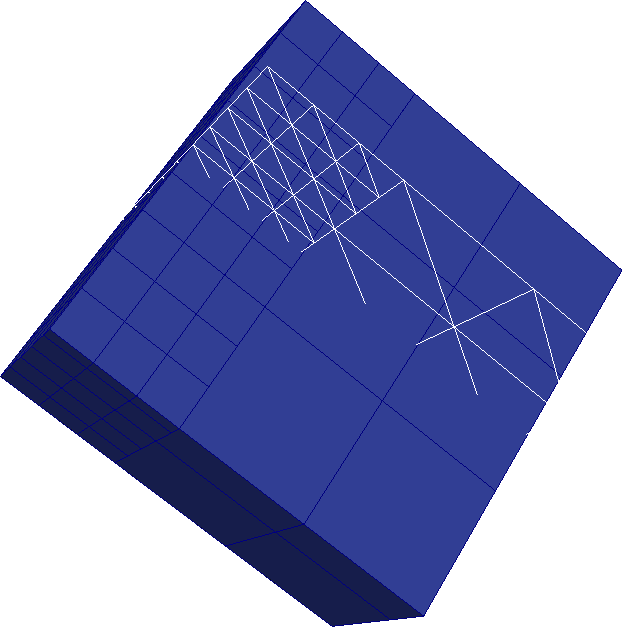
\includegraphics[width=0.4\textwidth]{41_heat-equation/dynamic00.png}
  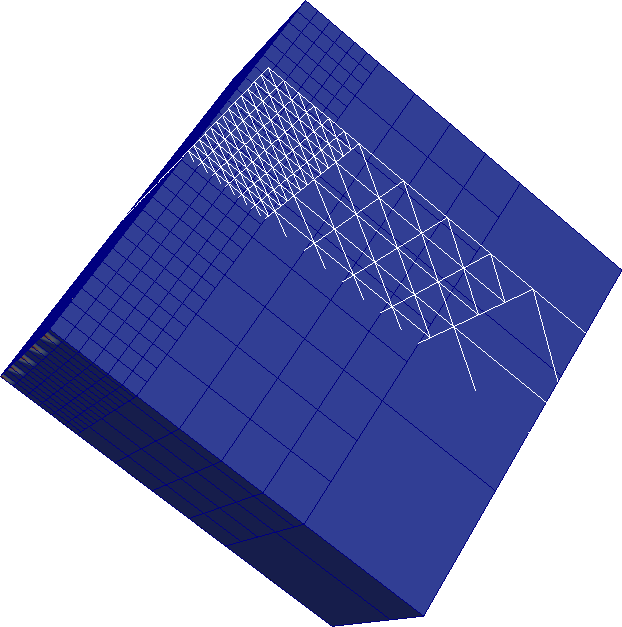
\includegraphics[width=0.4\textwidth]{41_heat-equation/dynamic01.png}
  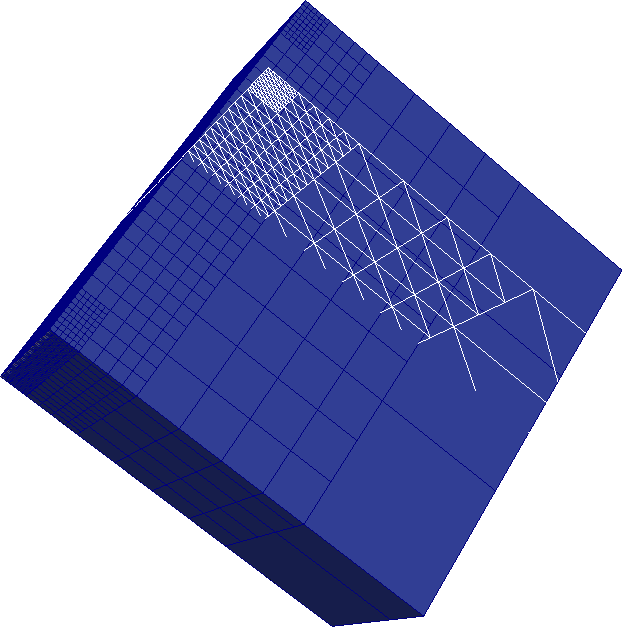
\includegraphics[width=0.4\textwidth]{41_heat-equation/dynamic02.png}
  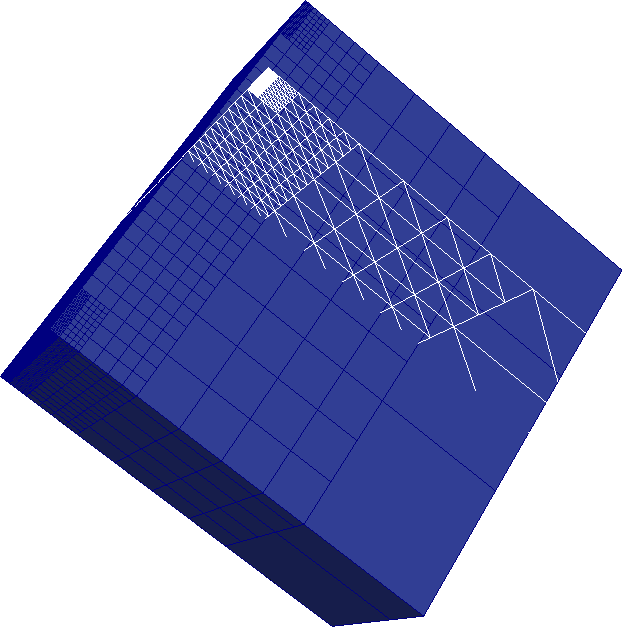
\includegraphics[width=0.4\textwidth]{41_heat-equation/dynamic03.png}
\end{center}


\subsection{Global data}

For most solvers, some kind of global information is required. 
Such data could be 
\begin{itemize}
  \item a global time step size,
  \item a residual norm,
  \item a counter for file plots, 
  \item and so forth.
\end{itemize}

\noindent
We could hold such information as static/global data in our code or as an
attribute in a mapping. 
Both options are not particular appealing. 
Global variables contradict our notion of nice decomposed programming.
Furthermore, I have to anticipate that Peano automatically replicates mappings
on a multithreaded system. 
So we have to be very carefully if we access global data within the mapping's
routines to avoid race conditions.
Attributes of mappings suffer from the same issues.
Furthermore, if mappings are replicated, they are replicated as well: 
instead of data races we have to ensure that data is correctly replicated and
then fused again. 
Finally, if we run on a distributed memory machine, multiple instances of our
application will execute because of MPI's SPMD paradigm, and we have to somehow
manually ensure that global data is kept consistent among all the ranks.


Peano's concept is to model all global data within the \texttt{State.def} file. 
Again, we can here also anticipate which data later on is to be distributed
between different ranks. We have discussed this issue before.
We also have clarified that the standard pattern is to set global data in the
runner through the State object and then to use this data alter on.

\begin{code}
Packed-Type: short int;


class myproject::dastgen::State {  
  persistent parallelise double dt;
};

\end{code}

To use a state, I recommend to make each mapping extract all required data from
the state in \texttt{beginIteration()}.
The idea is as follows (for parallel runs later on): a global algorithm control
routing sets global data in the state.
This state is distributed among all ranks.
All ranks run a particular set of mappings through one adapter.
Each mapping get the required data in \texttt{beginIteration()}.
Later on, we will can tune exactly when the state data is exchanged.

As copying attributes from the \texttt{State} object is laborious, a standard
pattern is to make each mapping hold a copy of the whole state:

\begin{code}
class myproject::mappings::TimeStep {
  private:
    /**
     * Logging device for the trace macros.
     */
    static tarch::logging::Log  _log;

    State _localState;
    ...
};
\end{code}

\noindent
It is important that this state is a local one and is overwritten in each run,
as the runner outside might have changed it.

\begin{code}
void myproject::mappings::TimeStep::beginIteration(
  myproject::State&  solverState
) {
  logTraceInWith1Argument( "beginIteration(State)", solverState );

  _localState  = solverState;
  _localState._clearAttributes(); // see remark below

  assertion2( _timeStepSize>0.0, _timeStepSize, solverState.toString() );

  logTraceOutWith1Argument( "beginIteration(State)", solverState);
}
\end{code}

\noindent
Once you need data from the state, you can extract this data within the mapping
via \linebreak \texttt{solverState.getTimeStepSize()} in the present example.


We finally have to clarify how to collect global data, i.e.~how to realise the
data flow the other way round. 
For this, we also use the copy of the state (this is only one implementation
pattern and again we could fill back data manually attribute-by-attribute. It
is just more convenient this way).
Usually, we first introduce an operation \texttt{State::clearAttributes()} that
resets all data, and we offer operations alike
\texttt{State::updateResidual(double myParam)} that allow us to collect
information within a \texttt{State} instance.

Within the mapping, we then use this operation to collect the data from all grid
entities:
\begin{code}
  ...
  _localState.updateResidual(myValue); 
  ...
\end{code}

\noindent
Obviously, the solution so far is not worth a penny, as the mappings work with
their own local copy of state. 
The solution now is to introduce a new operation 
\begin{code}
void State::merge( const State& otherState ) {
  _stateData.setMyLocalAttribute( 
    _stateData.getMyLocalAttribute() +
    otherState._stateData.getMyLocalAttribute() 
  ); 
}
\end{code}

\noindent
We call this operation in \texttt{endIteration()} to basically backplay the data
from the local copy into the global state:
\begin{code}
void myproject::mappings::TimeStep::endIteration(
  myproject::State&  solverState
) {
  solverState.merge( _localState );
}
\end{code}

\noindent
Finally, we can read the state in the global runner and plot some data to the
terminal, e.g.:
\begin{code}
int myproject::runners::Runner::runAsMaster(myproject::repositories::Repository& repository) {
  ...
  
  const double initialDt = 1e-4;
  repository.getState().setTimeStepSize( initialDt );
  for (int i=0; i<10000; i++) {
    if (i%100==0 || !repository.getState().isGridStationary()) {
      repository.switchToTimeStepAndPlot();
    }
    else {
     repository.switchToTimeStep();
    }
    repository.getState()._clearAttributes();
    repository.iterate();
    logInfo( "runAsMaster(...)", "my fancy global attribute=" <<
    repository.getState().getMyFancyGloalAttribute() );
    
    ...
  }
 
  ...
}
\end{code}

\noindent
Please note that you might have to clear also the global state from time to
time, which is done in the snippet above right before we call \texttt{iterate}.

\begin{remark}
  The whole process seems to be a little bit of overengineering just to get a
  few global variables right. The elegance of the solution becomes obvious when
  we use multiple MPI ranks and multiple threads. There, we rely on exactly the
  same \texttt{merge} operation to distribute a global state first to all ranks
  and threads before we fuse all distributed states together again into one
  object. 
\end{remark}

% 
%   \newpage
%   \section{Matrix-free multigrid}
  \label{section:applications:matrix-free-multigrid}

\chapterDescription
  {
    1--2 days.
  }
  {
    Chapter \ref{chapter:quickstart}. It is advantageous if the reader has
    studied the implementation of the heat equation before.
  }

In this section, we sketch how to solve the convection-diffusion equation
\[
  - \nabla (\epsilon \nabla) u + \nabla (v\ u) = f \qquad \mbox{with } v \in
  \mathbb{R}^d, \epsilon \in \mathbb{R}^{d \times d}
\]
with various geometric multigrid solvers. $epsilon$ is a diagonal matrix with
entries $\epsilon _1, \epsilon _2$ or $\epsilon _1, \epsilon _2, \epsilon _3$,
respectively.
Our realisation is based upon a few design decisions:

\begin{enumerate}
  \item The solvers use the spacetree as computational grid.
  \item We use a finite element formalism with $d$-linear shape functions.
  \item The material parameters $\epsilon $ and $v$ are given per cell.
\end{enumerate}


\noindent
For the implementation, we use Peano's \texttt{matrixfree} toolbox. 
This is a tiny little collection of helper classes to work with stencils and
local assembly matrix. 
It is neither fast, i.e.~computationally mature, nor can it cope with real
stencil libraries, but it does the job.



\subsection{Setup}

We start with Peano's PDT and generate a project. We also link Peano's sources
into the project and unzip the \texttt{matrixfree} toolbox. 
\begin{code}
  java -jar pdt.jar --create-project multigrid multigrid
  ln -s mypath/src/peano 
  ln -s mypath/src/tarch
  cp mypath/tarballs/toolboxes/matrixfree.tar.gz .
  tar -xzvf matrixfree.tar.gz
\end{code}


\noindent
I recommend to hold \texttt{matrixfree} parallel to the \texttt{multigrid},
\texttt{peano} and \texttt{tarch} directory.
As soon as we use such a toolbox, we also might have to adopt our makefile
accordingly: we have to add the matrixfree directory to the find pathes when we
build up a list of source codes.
Furthermore, you might have to add an additional search directory. If you place
your toolbox parallel to \texttt{peano} and \texttt{tarch}, this however should
not be necessary.
Here's the corresponding excerp from the makefile:
\begin{code}
files.mk:
    touch files.mk
    echo -n SOURCES= > files.mk
    find -H $(PEANO_HOME)/peano -name '*.cpp' | awk '{ printf "%s ", $$0 }' >> files.mk
    find -H $(PEANO_HOME)/tarch -name '*.cpp' | awk '{ printf "%s ", $$0 }' >> files.mk
    find -H $(PEANO_HOME)/matrixfree -name '*.cpp' | awk '{ printf "%s ", $$0 }' >> files.mk
    find $(PROJECT_HOME) -name '*.cpp' | awk '{ printf "%s ", $$0 }' >> files.mk
\end{code}

\noindent
We next add our material parameters to the \texttt{Cell.def} file
\begin{code}
Packed-Type: short int;

Constant: DIMENSIONS;

class multigrid::records::Cell {  
  persistent parallelise double   epsilon[DIMENSIONS];
  persistent parallelise double   v[DIMENSIONS];
};
\end{code}

\noindent
and create a simple first specification file:
\begin{code}
component: Multigrid

namespace: ::multigrid

vertex:
  dastgen-file: Vertex.def
  
cell:
  dastgen-file: Cell.def

state:
  dastgen-file: State.def

event-mapping:
  name: CreateGrid

event-mapping:
  name: PlotCells

adapter:
  name: CreateGrid
  merge-with-user-defined-mapping: CreateGrid
  merge-with-user-defined-mapping: PlotCells
  
\end{code}

\noindent
We run this specification file through the PDT

\begin{code}
java -jar <mypath>/pdt.jar --generate-gluecode multigrid/project.peano-specification multigrid
\end{code}


\noindent
and implement both the plotter and the creational mapping such that we have a
few characteristic setups. 
It might however make sense to validate that make passes before we start any
PDE-specific coding:
\begin{code}
make -f multigrid/makefile
\end{code}


\noindent
We next introduce an operation 
\begin{code}
matrixfree::stencil::ElementWiseAssemblyMatrix multigrid::Cell::getElementsAssemblyMatrix(
  const tarch::la::Vector<DIMENSIONS,double>&  h
) const {
  matrixfree::stencil::ElementWiseAssemblyMatrix result;

  const matrixfree::stencil::Stencil laplacianStencil = 
    matrixfree::stencil::getLaplacian(_cellData.getEpsilon(), h);

  return matrixfree::stencil::getElementWiseAssemblyMatrix(laplacianStencil);
}
\end{code}
which returns the $\mathbf{R}^{2^d \times 2^d}$ local system matrix. 
The method sets up the stencils that correspond to a regular Cartesian system
given the mesh size \textt{h} and the material parameters.
Here, also the convective term has to be handled.
Finally, it uses \texttt{getElementWiseAssemblyMatrix} to extract the actual
matrix from this stencil.

\begin{remark}
  Peano supports all stencil/linear algebra operations for complex values.
\end{remark}


\subsection{Jacobi smoother}

The basic building block of all of our solvers is a simple Jacobi smoother
working on adaptive grids as well as on multiple scales.
Its realisation is an extension of the solver in \ref{section:applications:heat-equation}.
To make it work without the assembly of any global matrix, we associate each
vertex a residual value as well as the actual value. 
There are a few other features such as boundary properties or some level
analysis that we either use later on or we pass to the used toolboxes. 
Their exact semantics and rationale have to be taken from the source code.

\begin{code}
Packed-Type: short int;


class multigrid::records::Vertex {  
  /**
   * Solution
   */
  persistent parallelise double  u;

  /**
   * Rhs
   */
  persistent parallelise double  f;
  
  /**
   * Residual
   */
  persistent parallelise double   r;

  /**
   * Diagonal element
   */
  persistent parallelise double   d;
  
  enum VertexType {
    Unknown, Dirichlet, Neumann
  };
  
  persistent VertexType vertexType;
  
  // some other attributes
};
\end{code}

\noindent
Besides a proper initialisation of the vertices, we extend the specification
similar to the heat equation.
\begin{code}
component: Multigrid

namespace: ::multigrid

vertex:
  dastgen-file: Vertex.def
  read scalar(double): U
  read scalar(double): R
  read scalar(double): D
  read scalar(double): F
  write scalar(double): U
  write scalar(double): R
  write scalar(double): D
  
...

adapter:
  name: CreateGrid
  merge-with-user-defined-mapping: CreateGrid
  merge-with-user-defined-mapping: PlotCells
  merge-with-predefined-mapping: VTKPlotVertexValue(u,getU,u)
\end{code}

\noindent
Once this code framework passes (only minor technical helper routines have to
be implemented, but by now this should be straightforward to any user), we can
introduce a new mapping/adapter \texttt{JacobiSmoother}, call this one a couple of hundred times in the runner and plot the result file then. 
For the latter, it makes sense to use a predefined plotter.
The interesting new aspects can be found in three routines of the smoother.
The design of the code realises matrix-free element-wise mat-vecs 1:1: 


\begin{enumerate}
  \item Each vertex carries a residual and a diagonal value attribute. 
    They are cleared whenever the vertex is read the very first time in
    a traversal.
    \begin{code}
void multigrid::mappings::JacobiSmoother::touchVertexFirstTime(...) {
  logTraceInWith6Arguments( "touchVertexFirstTime(...)", ... );

  fineGridVertex.clearAccumulatedAttributes();

  logTraceOutWith1Argument( "touchVertexFirstTime(...)", fineGridVertex );
}

// in Vertex files

void multigrid::Vertex::clearAccumulatedAttributes() {
  _vertexData.setR(0.0);
  _vertexData.setD(0.0);
}
    \end{code}
    
    \noindent
    Our concept is that we accumulate the diagonal element $d$ and the residual
    $r$ within these (temporary) attributes per vertex throughout the traversal.
    
    \item When we use a vertex for the very last time, we may thus update the
    unknown according to the values of the residual and the diagonal value. This
    is the actual Jacobi smoothing step:
    \[
      u ^{(new)} \gets u ^{(old)} + \omega \frac{1}{d} r
    \]
    \begin{code}
void multigrid::mappings::JacobiSmoother::touchVertexLastTime(...) {
  const bool hasUpdated = fineGridVertex.performJacobiSmoothingStep( omega );
  
  ...
}

// in Vertex files

double multigrid::Vertex::getResidual() const {
  return _vertexData.getF() + _vertexData.getR();
}


bool multigrid::Vertex::performJacobiSmoothingStep( double omega ) {
  if (
    getRefinementControl()==Vertex::Records::Unrefined
    &&
    _vertexData.getVertexType()== Records::Unknown
  ) {
    assertion1( _vertexData.getD()>0.0, toString() );
    assertion2( omega>0.0, toString(), omega );
    _vertexData.setU( _vertexData.getU() + omega / _vertexData.getD() * getResidual() );
    return true;
  }
  else {
    return false;
  }
}
    \end{code} 
    
    \noindent
    Please note that the residual here is modelled as sum of the right-hand
    side and the accumulated value (cf.~helper operation
    \texttt{getResidual()}).
    We anticipate the minus from the definition 
    \[ r = f - Au \]
    already in the accumulation, i.e.~sum up $-Au$ in the vertex attribute $r$.
    An additional pitfal is this context stems from the usage of a finite
    element method.
    It implies that we have to ensure that $f$ is scaled with $h^d$ ($h$ being the local mesh width), which is something we typically
    do already in the initialisation. 
    
    \begin{remark}
    It is obvious that the Jacobi update scheme may only update inner
    unrefined vertices as well as Neumann boundary points. Peano does not offer
    vertex types. It distinguishes only inner and outer vertices. As we need
    more flags than inside and outside (at least two boundary
    flags), we have to offer these on our own\footnotemark .
    \end{remark}
    \footnotetext{Up to
    early 2016, Peano had a three-valued logic with inner, outer and boundary vertices. I
    removed this from the kernel as most applications need way more vertex
    types anyway.}
    
    
    In the present implementation, we make the Jacobi update return a flag that
    indicates whether a fine grid update has been done or not. 
    Most codes will like to track global data such as a global residual or the
    maximum value of the solution and can use this flag to decide whether a
    vertex contributes to global data or not. Please study the accompanying
    source code for details.
    
    \item The most complicated part is obviously the evaluation of the local
    mat-vec contributions. Here, we rely on the cell's
    \texttt{getElementsAssemblyMatrix} as well as operations from \newline
    \texttt{VertexOperations}. All operations in this class are generated by the
    PDT and extract from \texttt{enterCell}'s vertices vectors: you hand in all
    fine grid data and extract a vector of all $u$ values, e.g. The other way
    round is supported as well. The operations within this helper class are all
    generated because of the read and write statements in the specification. 
    \begin{code}
#include "multigrid/VertexOperations.h"

void multigrid::mappings::JacobiSmoother::enterCell(...) {
  logTraceInWith4Arguments( "enterCell(...)", fineGridCell, ... );

  const tarch::la::Vector<TWO_POWER_D,double> u    =
    VertexOperations::readU( fineGridVerticesEnumerator, fineGridVertices );
  const tarch::la::Vector<TWO_POWER_D,double> dOld    =
    VertexOperations::readD( fineGridVerticesEnumerator, fineGridVertices );
  const tarch::la::Vector<TWO_POWER_D,double> rOld =
    VertexOperations::readR( fineGridVerticesEnumerator, fineGridVertices );
  const matrixfree::stencil::ElementWiseAssemblyMatrix A =
    fineGridCell.getElementsAssemblyMatrix( fineGridVerticesEnumerator.getCellSize() );

  tarch::la::Vector<TWO_POWER_D,double> r = rOld - A * u;
  tarch::la::Vector<TWO_POWER_D,double> d = dOld + tarch::la::diag(A);

  VertexOperations::writeR( fineGridVerticesEnumerator, fineGridVertices, r );
  VertexOperations::writeD( fineGridVerticesEnumerator, fineGridVertices, d );

  logTraceOutWith1Argument( "enterCell(...)", fineGridCell );
}
    \end{code}
\end{enumerate}



\subsection{Environment}

The changes in the environment are straightforward once the smoother is 
in place:
\begin{enumerate}
  \item We extend the runner such that it switches to the Jacobi smoother once 
  the grid is set up and triggers a fixed number of iterations then.
  \item We add a logging device to the runner
  \begin{code}
    class multigrid::runners::Runner {
      private:
        static tarch::logging::Log  _log;
        ...
    };
  \end{code}
  and make the innermost loop plot residual and other statistics after each 
  grid traversal:
  \begin{code}
  repository.switchToJacobiAndPlot();
  for (int i=0; i<100; i++) {
    repository.iterate();

    logInfo(
      "runAsMaster(...)",
      "#vertices=" << repository.getState().getNumberOfInnerLeafVertices() <<
      ",|res|_2=" << repository.getState().getResidualIn2Norm() <<
      ",|res|_max=" << repository.getState().getResidualInMaxNorm() <<
      ",|u|_L2=" << repository.getState().getSolutionInL2Norm() <<
      ",|u|_max=" << repository.getState().getSolutionInMaxNorm() <<
      ",#stencil-updates=" << repository.getState().getNumberOfStencilUpdates()
    );

    repository.getState().clearAccumulatedAttributes();
  }
  \end{code}
  \item To make the code work, we augment the state with the corresponding
  fields 
  \begin{code}
Packed-Type: short int;

class multigrid::records::State {  
  // Stores squared value, i.e. apply sqrt before returning it
  persistent parallelise double residual2Norm;
  persistent parallelise double residualMaxNorm;
  // Stores squared value, i.e. apply sqrt before returning it
  persistent parallelise double solutionL2Norm;
  persistent parallelise double solutionMaxNorm;
  persistent parallelise double numberOfStencilUpdates;
};
  \end{code}
  and realise the corresponding setters and getters. The design of the state
  methods (notably a method \texttt{clearAccumulatedAttributes()} in
  combination with \texttt{merge}) follows recommendations motivated in Section
  \ref{section:parallelisation:shared-memory}. For the time being, we do not
  discuss them further.
  \item Finally, we extend the \texttt{main} such that it can read in a
  well-suited relaxation parameter from the command line. It then sets this
  relaxation parameter (the static field) in the mapping:
  \begin{code}
    multigrid::mappings::JacobiSmoother::omega = atof( argv[2] );
  \end{code}
\end{enumerate}


\noindent
We may run this code for example the
well-known Poisson benchmark ($\epsilon = 1, v=0, f=d\ \pi ^2 \prod _i \sin
\left( x_i \pi \right) $ ), and observe the well-known dependency of Jacobi on
the mesh width (below grids with two, three or four compute grid levels):

\begin{center}
  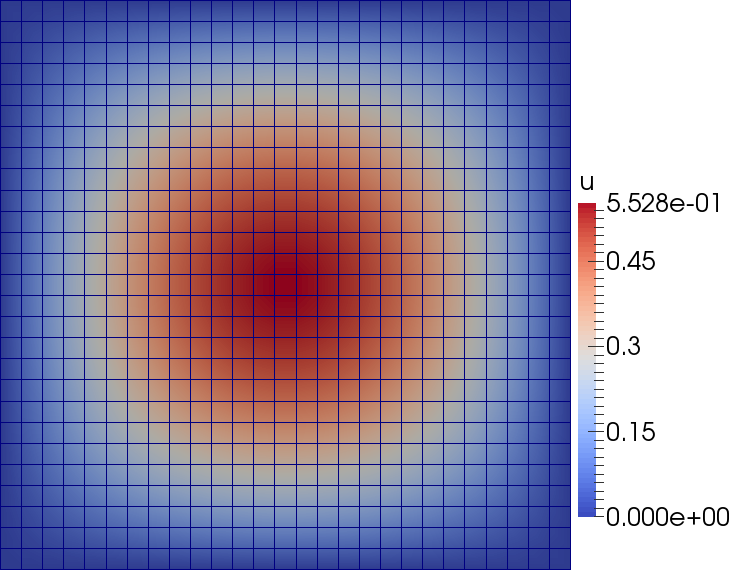
\includegraphics[width=0.3\textwidth]{42_matrix-free-multigrid/Poisson3.png}
  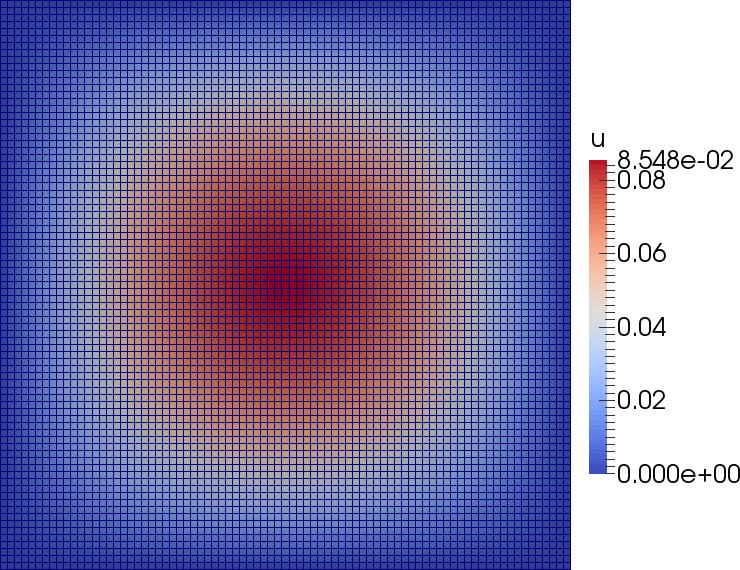
\includegraphics[width=0.3\textwidth]{42_matrix-free-multigrid/Poisson4.png}
  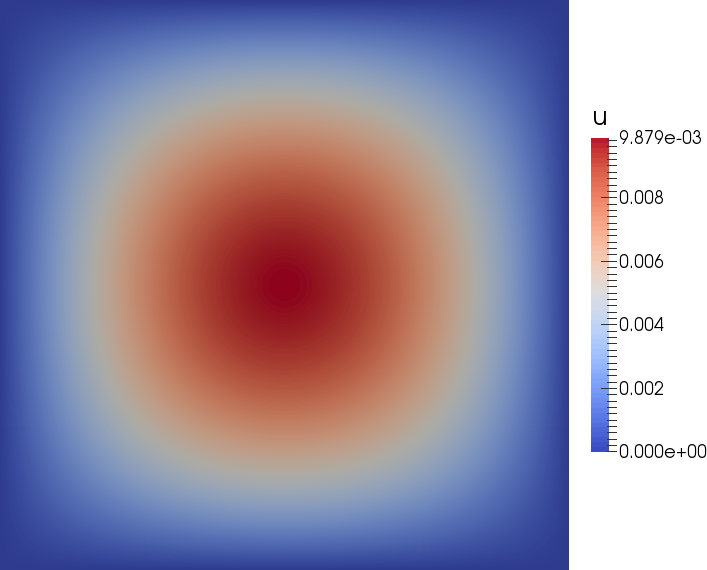
\includegraphics[width=0.3\textwidth]{42_matrix-free-multigrid/Poisson5.png}
\end{center}


\subsection{Dynamically adaptive Jacobi mit FAC}

\noindent 
We next implement a dynamically adaptive Jacobi solver that implements the FAC
scheme.
Its fundamental idea is that the Jacobi smootherr is applied on each and every
grid level in parallel.
Any hanging node's value is interpolated from coarser grids.
While we update all grid levels, we do overwrite coarse vertices with fine grid
values for all vertices that do exist on finer grid resolutions as well.
We inject the solution from the fine grids onto coarser grids.
This first solver is capable to handle dynamically adaptive grids with
arbitrary refinement pattern.
It also is a preliminary exercise how to implement multigrid full approximation
storage (FAS).

We extend the grid setup slightly such that it creates a very coarse grid even
if we prescribe a fine minimum mesh size.
Next, we validate that \texttt{enterCell} evaluates the stencil on each grid
level.
This leaves two tasks: interpolatation and injection.
The injection is basically the same we have used in the heat equation before.
\begin{code}
void multigrid::mappings::JacobiSmoother::touchVertexLastTime(...) {
 // see code snippets introduced before

 if (
  peano::grid::SingleLevelEnumerator::isVertexPositionAlsoACoarseVertexPosition(
    fineGridPositionOfVertex
  )
 ) {
  const peano::grid::SingleLevelEnumerator::LocalVertexIntegerIndex coarseGridPosition =
    peano::grid::SingleLevelEnumerator::getVertexPositionOnCoarserLevel
    (fineGridPositionOfVertex);
  coarseGridVertices[ coarseGridVerticesEnumerator(coarseGridPosition) ].inject(fineGridVertex);
 }
}


// in the vertex

void multigrid::Vertex::inject(const Vertex& fineGridVertex) {
  _vertexData.setU( fineGridVertex._vertexData.getU() );
}
\end{code}



\begin{remark}
  The \texttt{matrixfree} toolbox offers a type \texttt{solver::Smoother} that
  realises a Jacobi smoother that automatically tracks different residual and
  solution norms. In the present example we do not use this smoother while we
  use the toolbox's multigrid class. This is kind of inconsistent. It would
  probably be better to use the smoother as well.
\end{remark}

\noindent
The interpolation follows the idea of the heat equation solver, too.
However, we propose to rely on a premanufactured interpolation operation from
the \texttt{matrixfree} toolbox.
For this, we make our smoother mapping hold an instance of
\texttt{matrixfree::solver::Multigrid  \_multigrid}.
This object offers us an operation \texttt{getDLinearInterpolatedValue}: 

\begin{code}
void multigrid::mappings::JacobiSmoother::createHangingVertex(...) {
  logTraceInWith6Arguments( "createHangingVertex(...)", ... );

  fineGridVertex.setU(
    _multigrid.getDLinearInterpolatedValue(
      VertexOperations::readU( coarseGridVerticesEnumerator, coarseGridVertices ),
      fineGridPositionOfVertex
    )
  );

  logTraceOutWith1Argument( "createHangingVertex(...)", fineGridVertex );
}
\end{code}


\noindent
Obviously, the vertex requires an additional \texttt{setU( double )} operation
to make this snippet work.
Its implementation is trivial.
This is the only additional extension required.
If we adopt the setup, we might solve the equation on grids alike below where
the mesh is resolved up to the finest level along the boundaries. 
The latter is a proper choice for many problems, though inadequate and thus
only a proof of concept for the present case:

\begin{center}
  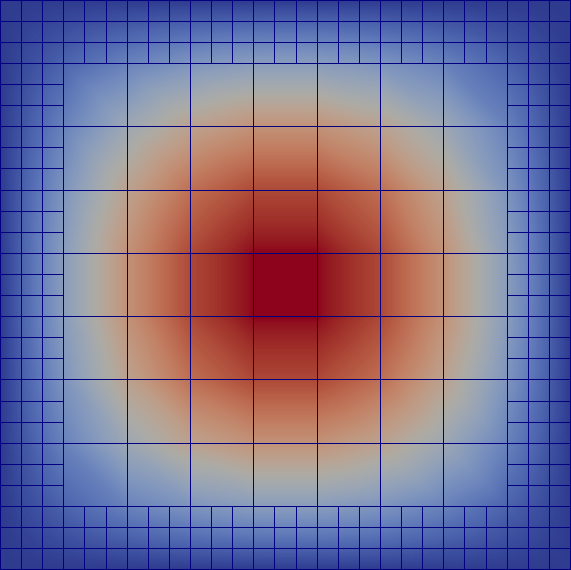
\includegraphics[width=0.3\textwidth]{42_matrix-free-multigrid/AdaptivePoisson3.png}
  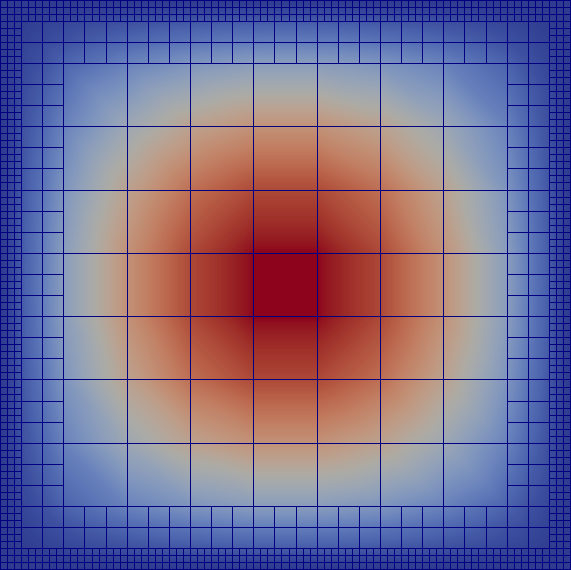
\includegraphics[width=0.3\textwidth]{42_matrix-free-multigrid/AdaptivePoisson4.png}
\end{center}



\begin{remark}
  On some machines, the resulting code will fail in \texttt{Assert} mode as the
  plotters complain about nan for the right-hand side. In the release
  mode, i.e.~without assertions, no complaint is raised, but some visualisation
  software might complain about the nans. To fix this issue with the plotting,
  it is important to set the right-hand side $f$ to zero for hanging nodes and
  for boundary nodes. We propose to introduce a \texttt{clearF()} operation and
  to call it prior to any plotting (in the \texttt{CreateGrid} mapping for
  example) for hanging and boundary vertices.
\end{remark}

\noindent
We close our discussion on the Jacobi smoother with the introducton of a dynamic
refinement criterion.
For this, we rely on a predefined refinement criterion offered with the
matrixfree toolbox.
We use
\texttt{LinearSurplusRefinementCriterionWithFixedMeshSizes}
from \\
\texttt{matrixfree::adaptivitycriteria}.
There is an extensive documentation how to use it in its superclass' header, so
we do not reiterate this here.
Instead we just show some of the added code:

\begin{code}
multigrid::mappings::RefinementCriterion::RefinementCriterion():
  _refinementCriterion(
    0.1,                   // refinementPercentage,
    0.0,                   // deletePercentage,
    0.5,                   // minimumMeshSize,
    0.5                    // maximumMeshSize
  ) {
}

void multigrid::mappings::RefinementCriterion::touchVertexFirstTime(...) {
  VertexOperations::writeLinearSurplus(fineGridVertex,0.0);
}

void multigrid::mappings::RefinementCriterion::enterCell(...) {
  VertexOperations::writeLinearSurplus(
    fineGridVerticesEnumerator,
    fineGridVertices,
    _refinementCriterion.getNewLinearSurplus(
      VertexOperations::readU(fineGridVerticesEnumerator,fineGridVertices),
      VertexOperations::readLinearSurplus(fineGridVerticesEnumerator,fineGridVertices)
    )
  );
}

void multigrid::mappings::RefinementCriterion::touchVertexLastTime(...) {
  if ( fineGridVertex.isInside() ) {
    const tarch::la::Vector<TWO_POWER_D_TIMES_D,double > coarseGridLinearSurplus =
      VertexOperations::readLinearSurplus(coarseGridVerticesEnumerator, coarseGridVertices)
      +
      _refinementCriterion.getLinearSurplusContributionFromFineGrid(
        VertexOperations::readLinearSurplus( fineGridVertex ),
        fineGridVertex.getRefinementControl()==Vertex::Records::Unrefined,
        fineGridPositionOfVertex
      );

    VertexOperations::writeLinearSurplus( coarseGridVerticesEnumerator, 
      coarseGridVertices, coarseGridLinearSurplus );

    switch (
      _refinementCriterion.analyse(
        VertexOperations::readLinearSurplus(fineGridVertex),
        fineGridVertex.getRefinementControl()==Vertex::Records::Refined,
        fineGridVertex.getRefinementControl()==Vertex::Records::Unrefined,
        fineGridH
      )
    ) {
      case matrixfree::adaptivitycriteria::LinearSurplusRefinementCriterion::Refine:
        fineGridVertex.refine();
        break;
      case matrixfree::adaptivitycriteria::LinearSurplusRefinementCriterion::Delete:
      case matrixfree::adaptivitycriteria::LinearSurplusRefinementCriterion::NoAction:
        break;
    }
  }
}
\end{code}

\noindent
The criterion's idea is to evaluate a stencil that allows us to compare the
linear interpoland of the solution within a vertex to the actual vertex's
solution value.
We anticipate what would happen if we could remove a particular vertex alone.
The other way round, we assume that vertices with a big difference are critical,
and we would benefit a lot if we would refine around this vertex.

The offered criterion class bucket sorts the linear surplus values. This is not
exact, but it does not require a real sort being in $\mathcal{O}(n \log
n)$---actually nothing is sorted, but each bucket is flagged (refine, coarse,
do nothing).
If a vertex falls into a particular bucket, the criterion returns the
corresponding flag.
More sophisticated criteria might yield better approximation patterns, but this
generic one works surprisingly well.

\begin{center}
  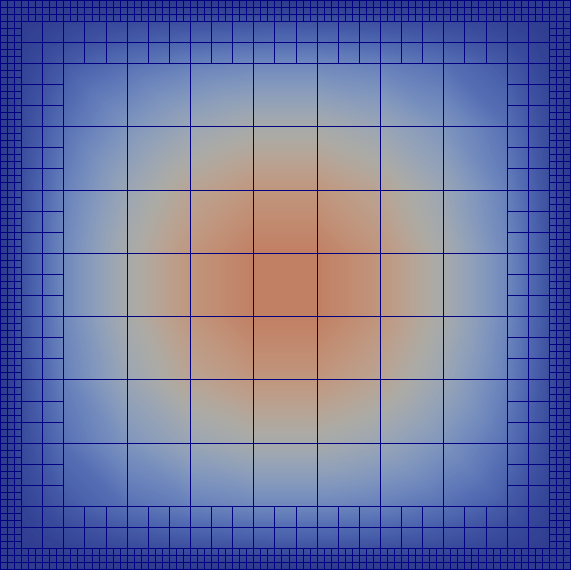
\includegraphics[width=0.24\textwidth]{42_matrix-free-multigrid/DynamicA00.png}
  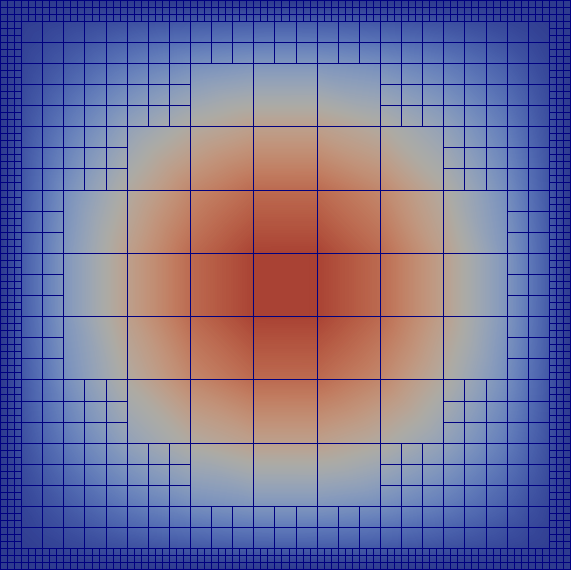
\includegraphics[width=0.24\textwidth]{42_matrix-free-multigrid/DynamicA01.png}
  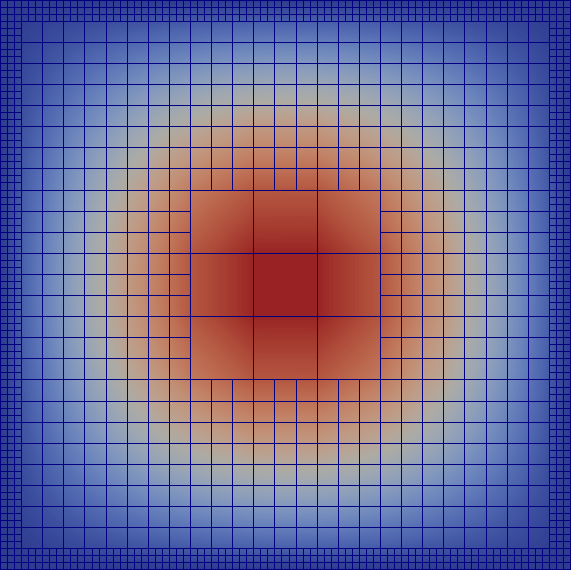
\includegraphics[width=0.24\textwidth]{42_matrix-free-multigrid/DynamicA02.png}
  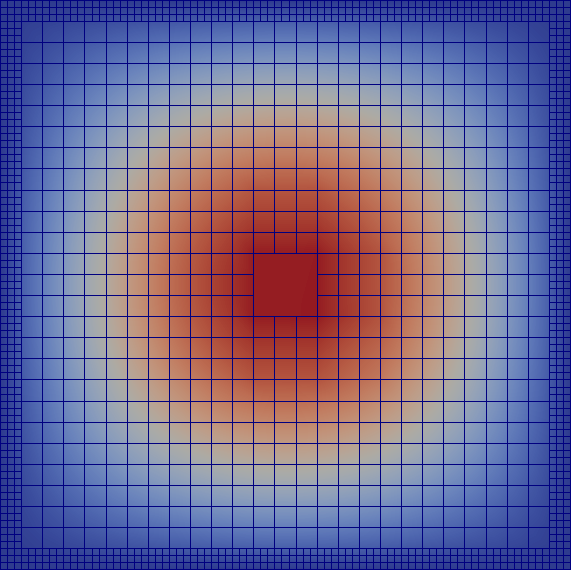
\includegraphics[width=0.24\textwidth]{42_matrix-free-multigrid/DynamicA03.png}
\end{center}

\noindent
This code marks up to ten percent of the vertices for refinemenet and
consequently refines all the surrounding cells given that the residual in
the vertices underruns the given threshold \\
\texttt{\_convergenceThreshold}.
The latter magic constant is set to $10^{-2}$ for the plots above.

Now, one simple feature is worth trying: We have so far always used a
predefined visualisation routine that visualises the finest grid of a
simulation.
Among the set of standard visualisation routines also is a plotter that plots
the individual levels of a grid.
Given that we inject the solution to coarse levels anyway, this allows us to
visualise all data in a multilevel fashion.
To use it, we again extend our specification, regenerate the glue code and
recompile.

\begin{code}
adapter:
  name: JacobiAndPlot
  merge-with-user-defined-mapping: CreateGrid
  merge-with-user-defined-mapping: JacobiSmoother
  merge-with-user-defined-mapping: PlotCells
  merge-with-predefined-mapping: VTKPlotVertexValue(u,getU,u)
  merge-with-predefined-mapping: VTKPlotVertexMultilevelValue(multiscaleU,getU,u)
\end{code}

\noindent
Some minor remarks on proper initialisation that are often encountered shall
close the discussion.
First, the presented refinement criterion does not properly refine along the
domain's boundary, as it does not distinguish whether a stencil is applied along
the boundary. 
In practice, it is reasonable to ensure that the boundary is always refined at
least as fine as the vertices next to the boundary. 
In practive, it is reasonable to avoid hanging vertices along the boundary. 
This can be achieved if we check within each cell whether there is a boundary
vertex and whether one vertex is refined.
If both properties hold, all unrefined boundary vertices have to be refined. 
The class \texttt{peano::grid::aspects::VertexStateAnalysis} provides generic
helper routines to realise this behaviour with a few lines:

\begin{code}
#include "peano/grid/aspects/VertexStateAnalysis.h"
#include "peano/utils/Loop.h"

void multigrid::mappings::RefinementCriterion::enterCell(...) {
  ...
  if (
    fineGridCell.isRefined()
    &&
    peano::grid::aspects::VertexStateAnalysis::doesOneVertexCarryRefinementFlag(
      fineGridVertices, fineGridVerticesEnumerator, Vertex::Records::Unrefined
    )
  ) {
    bool isOneVertexABoundaryVertex = false;
    dfor2(k)
      isOneVertexABoundaryVertex |= 
        fineGridVertices[ fineGridVerticesEnumerator(k) ].isBoundary();
    enddforx
    if (isOneVertexABoundaryVertex) {
      dfor2(k)
        if (fineGridVertices[ fineGridVerticesEnumerator(k) ].getRefinementControl()
          ==Vertex::Records::Unrefined) {
          fineGridVertices[ fineGridVerticesEnumerator(k) ].refine();
        }
      enddforx
    }
  }
 
}
\end{code}

\noindent
Second, many codes require a proper balancing. 
As Peano relies on three-partitioning, a 3:1 balancing is something many codes
would like to have: 
No two neighbouring cells differ in their maximum refinement level by more than
one.
This can be realised manually within a mapping. 
Or you may decide to merge the predefined mapping \texttt{GridBalancer3to1} into 
your adapters. 



Finally, any dynamically adaptive code should properly initialise new vertices. 
In the present example, a proper initialisation could rely on $d$-linear
interpolation again.
For multigrid, higher order schemes are desireable (though in practice I again
observed that linear interpolation is sufficient), but higher order
interpolation then has to be realised manually with helper variables or some
additional code applying the stencil to newly generated vertices.
We stick to the linear case here:
\begin{code}
void ...::createInnerVertex(...) {
  fineGridVertex.setU(
    _multigrid.getDLinearInterpolatedValue(
      VertexOperations::readU( coarseGridVerticesEnumerator, coarseGridVertices ),
      fineGridPositionOfVertex
    )
  );
}
\end{code}


\begin{center}
  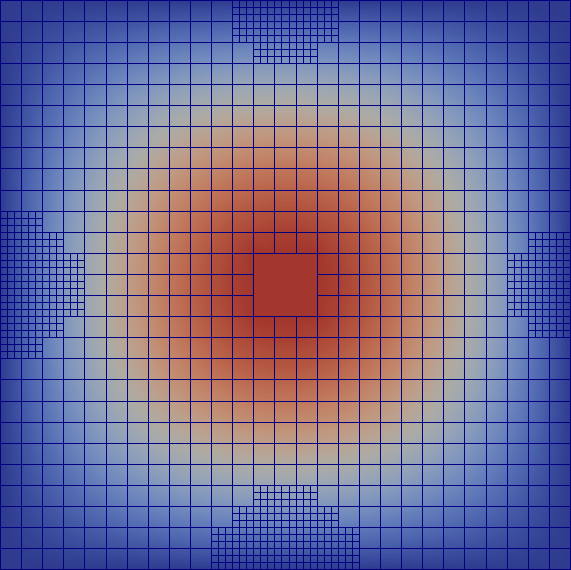
\includegraphics[width=0.34\textwidth]{42_matrix-free-multigrid/DynamicB.png}
  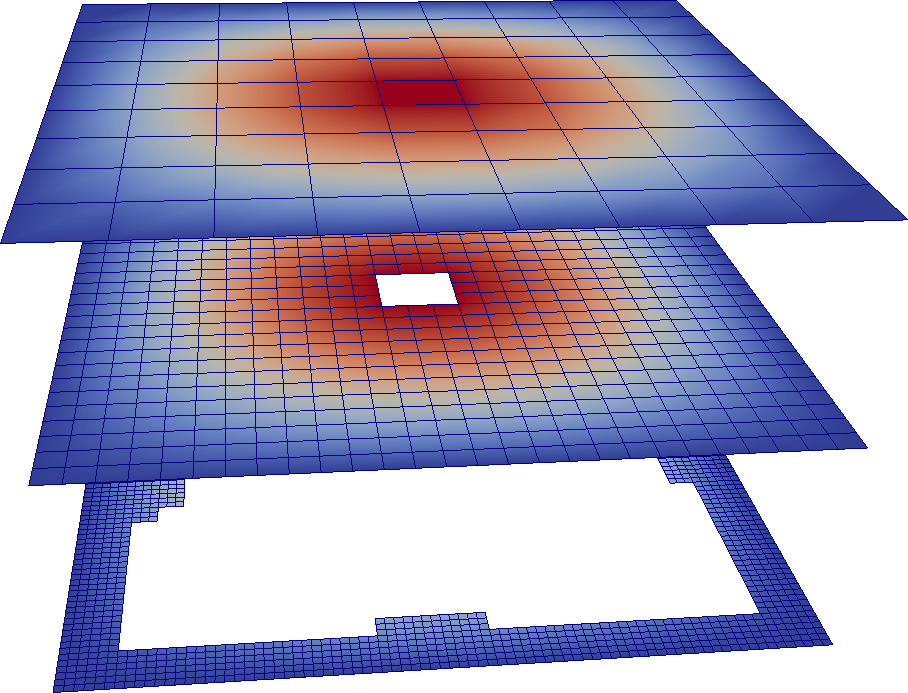
\includegraphics[width=0.45\textwidth]{42_matrix-free-multigrid/MultiLevel.png}
\end{center}

\noindent
The right image above presents the result of the multilevel plotter:
Each grid resolution level is written to a separate file.
It is obvious that finer grid solution approximations overwrite coarser vertex
values, while the coarse values determine the hanging node values.
We also see that the grid is refined towards the boundary here.



\subsection{Multigrid}

We start with some metaphilosophical considerations.
Multigrid algorithms work in two types of spaces: the ansatz
(discretisation) space holding the solution and a set of correction spaces.
The latter either are updated all at once (additive multigrid) or one after
another (multiplicative) before their contribution is added back to the actual
representation.
In the present discussion, we restrict ourselves to geometrically inspired
multigrid where both the correction and the discretisation space are spanned by
the spacetree's grid levels.
On the previous pages, we have realised a Jacobi directly within the
discretisation space without assembling any bigger matrix.
Obviously, such an approach also works for the correction equations.



At first glance, we then however need two variable sets per vertex: one set for
the actual discretisation and one for the correction equations.
As long as we work on regular grids only, there is no need to store different
types of variables within the vertices: refined vertices hold correction
equations, fine grid vertices hold the discretisation.
This approach becomes problematic for adaptive grids. 
Still, unrefined vertices of the fine grid hold the discretised PDE. 
On the same level of an arbitrary unrefined level, there might however also be
an area that is refined further.
Here, we solve a correction equation. 
If we realised both the correction equation and the discretisation with the same
set of variables, what would the right vertex values at the transition between
unrefined and correction areas be? 
We have to distinguish carefully in each cell which type of equation we are
solving, unless \ldots


\ldots we solve also the correction equation in a discretisation space. This is
the idea of full approximation storage (FAS) which fits perfectly to our
injection that we realised anyway. Instead of solving
\[ 
  A_{3h} e = \hat f 
\]
in areas that are refined further and thus hold a correction to the actual
solution iterate, we solve
\begin{eqnarray*}
  A_{3h} \left( Iu_h + e \right)  & = & \hat f +  A_{3h} Iu_h \qquad \mbox{added
  an additional term on both sides} \\
  & = & R r_h + RA_hPIu_h \\
  & = & R \left( r_h + A_hPIu_h \right) \\
  & = & R \left( f_h - A_hu_h + A_hPIu_h \right) \\
  & = & R \left( f_h - A_h\left( id - PI\right)u_h \right) \\
  & =: & R \left( f_h - A_h \hat u_h \right)  =: R \hat r_h  
\end{eqnarray*}
i.e.~work with a coarsened solution as input to the correction solve 
which is a formalism introduced by Griebel as HTMG.


So we can stick to our injections of the solution. 
In each traversal, we have to determine the hierarchical surplus in each vertex
$\hat u = u - PIu_h$ which is simple, as $Iu_h$ is available anyway.
This hierarchical transform is a temporary helper. 
We can throw it away after the traversal again.
We can model it as \texttt{discard} in the \texttt{Vertex.def}.

Once we have $\hat u$, we can simultaneously determine the residual $r$ as well
as its hierarchical counterpart $\hat r$. 
With the residual $r$, we update the solution if we have to---a detail subject
of discussion in a minute when we finalise whether to realise a multiplicative
or additive scheme.
The hierarchical residual $\hat r$ in turn is not used to update any solution
directly.
It is restricted to the next coarser level to yield a right-hand side there.


We finally observe that we may not just update the solution with the residual.
If we did that we would loose the knowledge which correction to prolong to the
next finer level.
We therefore store the updates in another helper variable and use this update to
prolong it to a finer level later on.

\begin{remark}
  The update helper variable obviously is not the only valid choice to
  distinguish coarse grid updates from fine grid representation. It is obviously
  that we also might store the hierarchical surplus persistently and then
  reconstruct the nodal value with the relation $u_h=\hat u_h+Pu_{3h}$. This is
  the implementation variant discussed in (Weinzierl:09), while a more detailed
  analysis of required helper variables for additive multigrid can be found in
  (Reps:16).
\end{remark}



\begin{code}
class multigrid::records::Vertex {  
  persistent parallelise double  u;             // Solution
  persistent parallelise double  f;             // Rhs
  discard parallelise double     r;             // Residual
  discard parallelise double     d;             // Diagonal element
  discard parallelise double     hierarchicalU; // Hierarchical solution
  discard parallelise double     hierarchicalR; // Hierarchical residual
  persistent parallelise double  uUpdate;       // Update of solution
  discard parallelise double     linearSurplus[DIMENSIONS];

  enum VertexType {
    Unknown, Dirichlet, Neumann
  };
  persistent VertexType vertexType;
};
\end{code}


\noindent
The hierarchical surplus has to be determined in \texttt{touchVertexFirstTime}
where we also clear the temporary variables.
I decided to realise the generic multigrid operations in a mapping of its own. 
It is called \texttt{HierarchicalTransformAndRHSRestriction}.
Once more, we rely on an instance of the Multigrid class.

\begin{code}
void
multigrid::mappings::HierarchicalTransformAndRHSRestriction::createHangingVertex(...) { 
  fineGridVertex.clearHierarchicalValues();
}

void multigrid::mappings::HierarchicalTransformAndRHSRestriction::touchVertexFirstTime(...) {
  fineGridVertex.clearHierarchicalValues();

  if ( fineGridVertex.isInside() ) {
    const tarch::la::Vector<TWO_POWER_D,double > u_3h  = VertexOperations::readU
      (coarseGridVerticesEnumerator,coarseGridVertices);
    const double                                 Pu_3h = _multigrid.getDLinearInterpolatedValue
      (u_3h,fineGridPositionOfVertex);

    fineGridVertex.determineUHierarchical(Pu_3h);

    if (fineGridVertex.getRefinementControl()!=Vertex::Records::Unrefined) {
      fineGridVertex.clearF();
    }
  }
}

void multigrid::Vertex::determineUHierarchical(double Pu_3h) {
  _vertexData.setHierarchicalU( _vertexData.getU()-Pu_3h );
}
\end{code}



\noindent
The accumulation of the hierarchical surplus itself is more or less a
cut-n-paste from the Jacobi smoother:
\begin{code}

void multigrid::mappings::HierarchicalTransformAndRHSRestriction::enterCell(...) { 
  const tarch::la::Vector<TWO_POWER_D,double> hierarchicalU    =
     VertexOperations::readHierarchicalU( fineGridVerticesEnumerator, fineGridVertices );
   const tarch::la::Vector<TWO_POWER_D,double> hierarchicalROld =
     VertexOperations::readHierarchicalR( fineGridVerticesEnumerator, fineGridVertices );
   const matrixfree::stencil::ElementWiseAssemblyMatrix A =
     fineGridCell.getElementsAssemblyMatrix( fineGridVerticesEnumerator.getCellSize() );

   tarch::la::Vector<TWO_POWER_D,double> hierarchicalR = 
     hierarchicalROld - A * hierarchicalU;

   VertexOperations::writeHierarchicalR
     ( fineGridVerticesEnumerator, fineGridVertices, hierarchicalR );
}
\end{code}

\noindent 
For the restriction, we again rely on the multigrid object, where a specialised
prolongation function does exist that uses $d$-linear interpolation.
Furthermore, we stick to the convention $R=P^T$ and thus can write:

\begin{code}
void
multigrid::mappings::HierarchicalTransformAndRHSRestriction::touchVertexLastTime(...) {
  if ( fineGridVertex.isInside() ) {
    const tarch::la::Vector<TWO_POWER_D, double > P = 
      _multigrid.calculateP(fineGridPositionOfVertex);

    dfor2(k)
      // There is no need to exclude boundary points here (the rhs does not play
      // there a role anyway), but it makes the visualisation nicer.
      if (
        coarseGridVertices[ coarseGridVerticesEnumerator(k) ].getRefinementControl()==
          Vertex::Records::Refined
        &&
        coarseGridVertices[ coarseGridVerticesEnumerator(k) ].isInside()
      ) {
        coarseGridVertices[ coarseGridVerticesEnumerator(k) ].incF(  
          P(kScalar) * fineGridVertex.getHierarchicalResidual() 
        );
      }
    enddforx
  }
}

void multigrid::Vertex::incF(double value) {
  _vertexData.setF( _vertexData.getF()+value );
}

double multigrid::Vertex::getHierarchicalResidual() const {
  return _vertexData.getF() + _vertexData.getHierarchicalR();
}

bool multigrid::Vertex::performJacobiSmoothingStep( double omega ) {
  if ( _vertexData.getVertexType()== Records::Unknown ) {
    assertion1( _vertexData.getD()>0.0, toString() );
    assertion2( omega>0.0, toString(), omega );
    const double update = omega / _vertexData.getD() * getResidual();
    _vertexData.setU( _vertexData.getU() + update );
    _vertexData.setUUpdate( update );
     return getRefinementControl()==Vertex::Records::Unrefined;
  }
  else {
    return false;
  }
}
\end{code}


\noindent
We note that the new Jacobi update works on all vertices on all grid levels. 
The result clearly indicates that only updates on the finest grid level may
contribute to the calculation of the global residual, i.e.~any smoother should
check the result and update global values if and only if
\textttt{performJacobiSmoothingStep} returns true.


We close the preparatory work with the remark that the specification has to be
augmented by additional readers and writers to make our code snippets work:

\begin{code}
component: Multigrid

namespace: ::multigrid

vertex:
  dastgen-file: Vertex.def
  read scalar(double): U
  read scalar(double): F
  read scalar(double): R
  read scalar(double): D
  read scalar(double): HierarchicalU
  read scalar(double): HierarchicalR
  write scalar(double): U
  write scalar(double): R
  write scalar(double): D
  write scalar(double): HierarchicalU
  write scalar(double): HierarchicalR

...
\end{code}

\begin{center}
  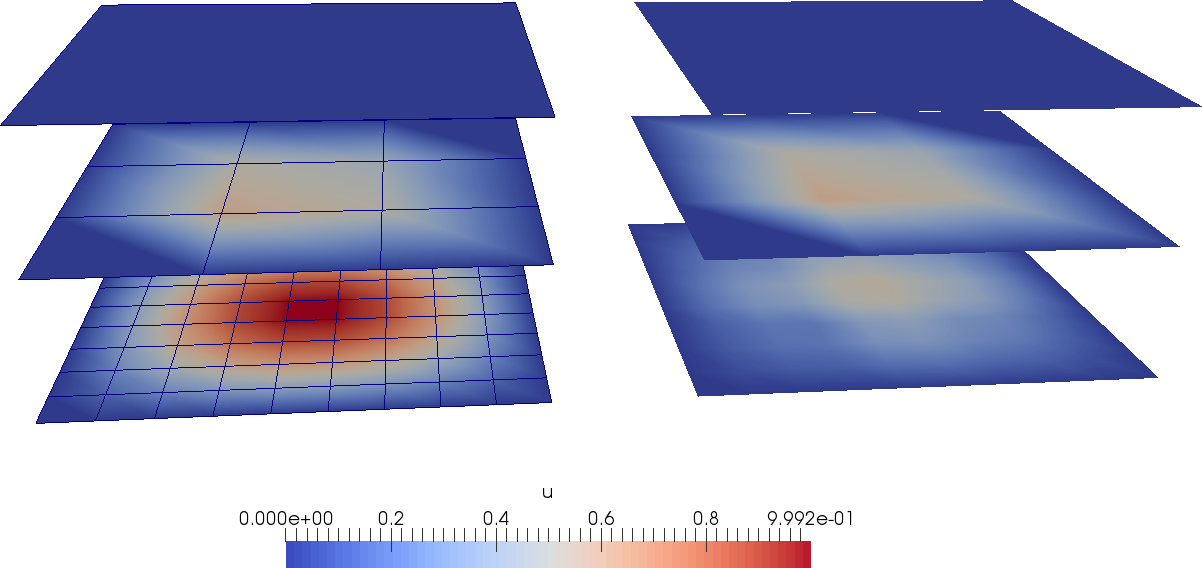
\includegraphics[width=0.8\textwidth]{42_matrix-free-multigrid/Hierarchical-Jacobi.png}
\end{center}

\noindent
We see above a Jacobi smoother (100 iterations) for the Poisson equation on the
unit square (left) as well as the hierarchical representation (right).
We also may augment the adapters with plots of the temporary data 

\begin{code}
adapter:
  name: AnyAdapter
  ...
  merge-with-predefined-mapping: VTKPlotVertexValue(u,getU,u)
  merge-with-predefined-mapping: VTKPlotVertexMultilevelValue(multiscaleU,getU,u)
  merge-with-predefined-mapping: VTKPlotVertexMultilevelValue
    (multiscaleHierarchicalU,getHierarchicalU,u)
  merge-with-predefined-mapping: VTKPlotVertexMultilevelPointCloud
    (multiscaleResidual,getResidual,res)
  merge-with-predefined-mapping: VTKPlotVertexMultilevelPointCloud
    (multiscaleHierarchicalResidual,getHierarchicalResidual,res)
  merge-with-predefined-mapping: VTKPlotVertexMultilevelPointCloud(f,getF,f)
\end{code}

\noindent
and note that we basically have almost all multigrid ingreditents at hands.
Missing is a projection from coarse grid updates to fine grid values.
So far, we update the coarse grid values according to the right-hand side.
These updates however are not projected.
Instead, the updated approximation in a FAS sense are overwritten at the end of
the subsequent iteration with fine grid solution data. 


\begin{remark}
  Most default VTK plotters plot the grid as well as values and (for
  consistency reasons imposed by the VTK data file format) have to plug into
  \texttt{touchVertexFirstTime}. For residuals and other temporary data, we
  typically however are interested to plot the value at the end of the
  iteration. A quick solution here is to plot the grid with one mapping and to
  use a second mapping that solely plots a point cloud with the vertex values.
  We then can visualise both data sets simultaneously.
\end{remark}

\subsection{Additive Geometric Multigrid}

In additive multigrid, we may not use the same relaxation factor on each and
every level. 
Instead, it is important that the coarser the level the smaller the contribution
to the solution update.
Otherwise, the solver tends to overshoot and become unstable. 
We propose to use relaxation factors $\omega ^k$ with $k=1$ on the fine grid
level and increasing by one for each level up the hierarchy.
$\omega $ obviously has to be adopted if the grid changes.
It is thus straightforward to compute it on-the-fly. 
For this, we add an additional variable to the vertex

\begin{code}
class multigrid::records::Vertex {  
  persistent parallelise int  numberOfFinerLevelsAtSamePosition;
};
\end{code}

\noindent
and make the grid traversal determine the correct value of this attribute
on the fly:



@todo Instabil. Relaxation mit aufnehmen

@todo Kleiner Fehler mit der Injektion. Auf Bram verweisen, aber so lassen







\subsection{Multiplicative Geometric Multigrid}

V2,2?




\subsection*{Further reading}

\begin{itemize}
  \item  Reps, Bram and Weinzierl, Tobias: {\em Complex additive geometric
  multilevel solvers for Helmholtz equations on spacetrees}, tech report,  
  arXiv:1508.03954
  \item Weinzierl, Marion: {\em Hybrid Geometric-Algebraic Matrix-Free Multigrid on
Spacetrees}, Dissertation, Technische Universit\"at M\"unchen, 2013
  \item   Muntean, Ioan Lucian, Mehl, Miriam, Neckel, Tobias and Weinzierl,
  Tobias (2008). {\em Concepts for Efficient Flow Solvers Based on Adaptive
  Cartesian Grids}. In High Performance Computing in Science and Engineering, Garching 2007. Wagner, Siegfried, Steinmetz, Matthias, Bode, Arndt & Brehm, Matthias Berlin Heidelberg New York: Springer.
  \item Weinzierl, Tobias and K\"oppl, Tobias (2012). {\em A Geometric
  Space-time Multigrid Algorithm for the Heat Equation}. Numerical Mathematics:
  Theory, Methods and Applications 5(1): 110-130.
  \item Mehl, Miriam, Weinzierl, Tobias and Zenger, Christoph (2006). {\em A
  cache-oblivious self-adaptive full multigrid method}. Numerical Linear Algebra
  with Applications 13(2-3): 275-291.
\end{itemize}

%   \newpage
%   \section{Diffusion-convection with PETSc}
  \label{section:applications:petsc}

\chapterDescription
  {
    60 minutes.
  }
  {
    Chapter \ref{chapter:quickstart} and a working PETSc installation.
  }

I wrote Peano with matrix-free methods from CFD in mind. 
It turns out that it is not too complicated to use it for other application
areas or to established linear algebra packages.
We assume that you have PETSc plus BLAS, Lapack and MPI (if required) ready
installed on your system.
I have tested all the present concepts with PETSc 3.7.2 but everything discussed
here is pretty basic, so it should work with older versions as well.
Please note that this is a feasibility study and we do not optimise at all.


\subsection{Preparation of Peano}

If we use explicit assembly, we need an enumeration of our grid. 
So we do start with a grid
\begin{code}
> java -jar <mypath>/pdt.jar --create-project petsc chapter-4.3
\end{code}

\noindent
and add each vertex an index. 
We do restrict to a discretisation with one degree of freedom per vertex for the
time being:

\begin{code}
Packed-Type: short int;

class petsc::records::Vertex {  
  parallelise persistent int index;
};
\end{code}

\noindent
For the present exercise, we will have four different things to do:
create the grid, create and assemble the matrix, solve the problem and plot the
result.
The solve is a pure PETSc operation.
For each of the remaining three phases, we need a mapping/adapter in Peano and
we also want access to \texttt{index}.
For the latter, we could write setters and getters and stick to an
object-oriented paradigm.
But this way, it is easier (though not as beautiful):

\begin{code}
component: MyFancyPETScProject

namespace: ::petsc

vertex:
  dastgen-file: Vertex.def
  read scalar(int): Index   // mind the uppercase
  write scalar(int): Index
  
cell:
  dastgen-file: Cell.def

state:
  dastgen-file: State.def

event-mapping:
  name: CreateGrid

event-mapping:
  name: Assemble

adapter:
  name: CreateGrid
  merge-with-user-defined-mapping: CreateGrid

adapter:
  name: Assemble
  merge-with-user-defined-mapping: Assemble
 
adapter:
  name: Plot
  merge-with-predefined-mapping: VTKPlotVertexValue(result,getU,u)
\end{code}

We generate all glue code
\begin{code}
> java -jar <mypath>/pdt.jar --generate-gluecode \
  petsc/project.peano-specification petsc <mypath>/pdt/usrtemplates
> make -f petsc/makefile
\end{code}

\noindent
We recognise that this code does not compile yet as we have not yet realised \texttt{double Vertex::getU() const}.
For the time being, we make the routine return 0.
Finally, we change into the mapping the creational events yield a regular grid:

\begin{code}
void petsc::mappings::CreateGrid::createInnerVertex(...) {
  logTraceInWith6Arguments( "createInnerVertex(...)", ... );

  if (coarseGridVerticesEnumerator.getLevel()<3) {
	fineGridVertex.refine();
  }

  logTraceOutWith1Argument( "createInnerVertex(...)", fineGridVertex );
}


void petsc::mappings::CreateGrid::createBoundaryVertex(...) {
  logTraceInWith6Arguments( "createBoundaryVertex(...)", ... );

  if (coarseGridVerticesEnumerator.getLevel()<3) {
	fineGridVertex.refine();
  }

  logTraceOutWith1Argument( "createBoundaryVertex(...)", fineGridVertex );
}
\end{code}

\noindent
Compile it, run it, visualise the output.


\subsection{Connecting to PETSc}

As PETSc's philosophy is pretty straightforward and minimalistic (they do, e.g.,
not hijack the main), the initialisation and integration are straightforward.
Please note that we stick to serial jobs in the first part of this section.
Nevertheless, we use the MPI compiler wrapper to translate the code as I faced
issues when I tried to use PETSc without MPI\footnote{Please consult
\url{http://www.mcs.anl.gov/petsc/petsc-current/docs/installation.html#i-dont-want-to-use-mpi}
for the usage with OpenMPI as the \texttt{LD\_LIBRARY\_PATH} has to be set
properly.}.


\begin{enumerate}
  \item Before we start to code with PETSc, we have to make the makefile know
  where PETSc is installed. If you use your own build environment, adopt all
  pathes accordingly. If you use the pre-generated makefile, open it and add
  your PETSc include directory to the search path. Also switch to
  \texttt{mpiCC}.
  \begin{code}
    PROJECT_CFLAGS = -DDebug -DAsserts -DParallel \
      -DMPICH_IGNORE_CXX_SEEK -I/opt/petsc/include 
    PROJECT_LFLAGS = -L/opt/petsc/lib -lpetsc 
    PROJECT_LFLAGS = -L/opt/petsc/lib -lpetsc

    [...]

    CC=/opt/openmpi/bin/mpiCC
  \end{code}
  Please adopt all pathes accordingly. Depending on your MPI version, you also
  might run into issues with the compiler's error management. I recommend to
  remove \texttt{-Werror -pedantic-errors} from your makefile in this case.
  \item As the present PETSc solutions use MPI (through they run serially), we
  have to make a few modifications in the runner. These modifications are
  detailed in Chapter \ref{section:parallelisation:mpi}, so we simply show
  what has to be changed in \texttt{runners/Runner.cpp}. This solution should
  work out-of-the-box.
  For a description of its semantics, please see the aforementioned chapter.
  \begin{code}
#include "tarch/parallel/FCFSNodePoolStrategy.h"
#include "peano/parallel/loadbalancing/OracleForOnePhaseWithGreedyPartitioning.h"

[...]

int petsc::runners::Runner::run() {

  [...]

  petsc::repositories::Repository* repository = 
    petsc::repositories::RepositoryFactory::getInstance().createWithSTDStackImplementation(
      geometry,
      tarch::la::Vector<DIMENSIONS,double>(1.0),   // domainSize,
      tarch::la::Vector<DIMENSIONS,double>(0.0)    // computationalDomainOffset
    );
  

  // This is new because of PETSc:
  if (tarch::parallel::Node::getInstance().isGlobalMaster()) {
    tarch::parallel::NodePool::getInstance().setStrategy(
      new tarch::parallel::FCFSNodePoolStrategy()
    );
  }
  tarch::parallel::NodePool::getInstance().restart();
  tarch::parallel::NodePool::getInstance().waitForAllNodesToBecomeIdle();
  peano::parallel::loadbalancing::Oracle::getInstance().setOracle(
    new peano::parallel::loadbalancing::OracleForOnePhaseWithGreedyPartitioning(false)
  );

  [...]
}
  \end{code}
  \item Finally, we have to initialise and shut down PETSc properly in
  \texttt{main.cpp}:
  \begin{code}
#include "petscsys.h"

[...]

int main(int argc, char** argv) {
  [...]
  PetscInitialize(&argc,&argv,(char*)0,(char*)0);

  int programExitCode = 0;

  if (programExitCode==0) {
    [...]
    petsc::runners::Runner runner;
    programExitCode = runner.run();
  }

  PetscFinalize();
  [...]
}  
  \end{code}
  According to PETSc's documentation, we could use PETSc's initialisation to set
  up MPI instead of the Peano initialisation. However, Peano's initialisation
  does not check whether MPI has been set up before where PETSc does. So it
  makes sense to initialise Peano first.
\end{enumerate}




\subsection{Setting up the PETSc data structures}

Once we have created the grid (and perhaps visualised it), we can start to set
up the PETSc data structures corresponding to the grid. 
We stick to the regular case for the time being.

Every fine grid vertex in the grid has a right-hand side and a solution entry. 
Different to previous sections, we do not store this data in the vertex.
Instead, we will make PETSc hold two vectors $rhs$ and $x$ and
make each vertex hold the index, i.e.~each vertex knows which entry in the two
vertices is associated with the vertex.



@todo Discuss the whole Assemble.cpp as well as the header.

#include "petscvec.h"



\subsection{Serial assembly with a parallel PETSc}


\subsection{Using PETSc and MPI}
% others. So it is a perfect fit to Peano.


%   \newpage
%   \section{A patch-based heat equation solver}


\chapterDescription
  {
    60 minutes.
  }
  {
    Chapter \ref{chapter:quickstart}.
  }

In this section, we sketch how to realise a simple explicit heat equation
solver that is based upon patches.
The idea is that we embed a small regular Cartesian grid into each individual
spacetree leaf.
This patch is surrounded by a halo/ghost cell layer holding copies from
neighbouring patches.

\begin{center}
  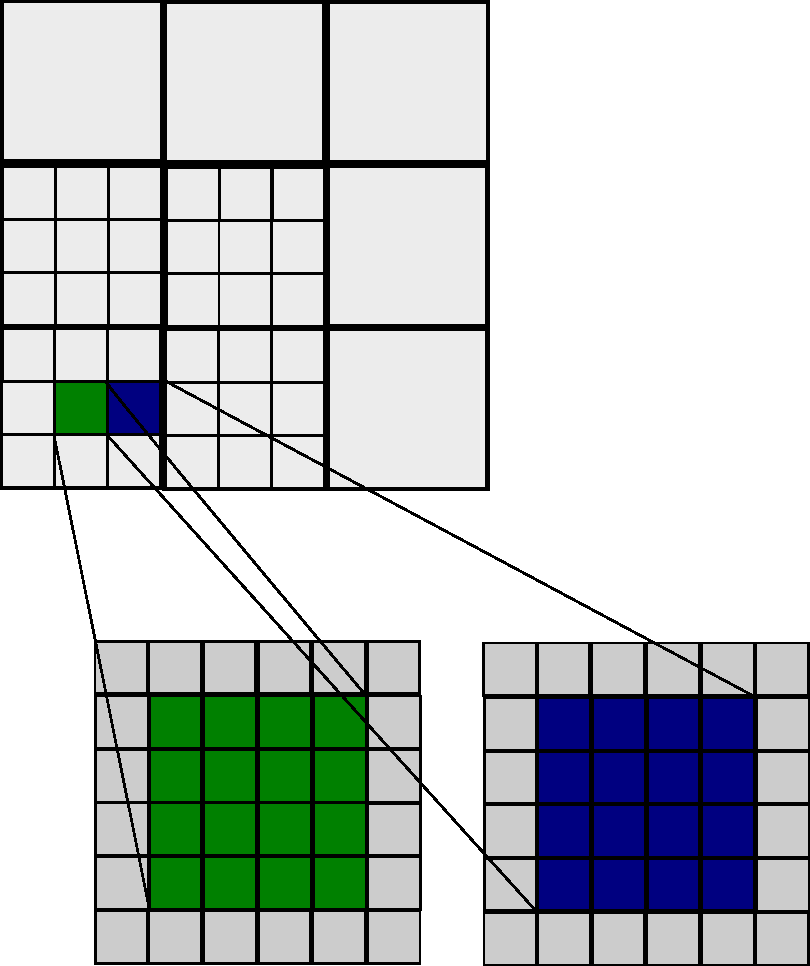
\includegraphics[width=0.4\textwidth]{44_patch-based-solver/patches.pdf}
\end{center}

In the sketch, we enbed $4\times 4$ patches into the spacetree cells.
Two cells (blue and green) are illustrated.
Each patch is surrounded by a halo layer of size one.
We will write the code to work within the patches, while the layers around the
patches will hold copies of the neighbouring patches and thus couple them.

For this endeavour, we need the toolbox \texttt{multiscalelinkedcell} that you
can download from the Peano webpage.
We assume that the whole toolbox is unzipped into a directory
\texttt{multiscalelinkedcell} which is held by your source directory.


\subsection{Preparation}

We start with the creation of a file \texttt{PatchDescription.def} in your
project's root directory. 
In our example, each patch solely shall hold one array of unknowns $u$ that are
associated to the vertices of the patch.
So each patch will have exactly $(4+2+1)^2$ unknowns (the four is the size,
there's two halo cells along each coordinate axis, and then there's finally one
more vertex than there are cells).
Besides the unknowns called $u$, we also store the position and size as well as
the level with each patch---well-aware that level and size are kind of
redundant.

\begin{code}
#include "peano/utils/Globals.h"

Packed-Type:  int;

Constant: DIMENSIONS;

/**
 * A cell description describes one individual patch of the overall grid, i.e. 
 * it holds pointers to the actual data of the patch (arrays) and its meta data
 * such as time stamps. Each unrefined node of the spacetree, i.e. each leaf, 
 * holds exactly one instance of this class. 
 */
class myprojectname::records::PatchDescription {
  /**
   * Two pointers to float arrays.
   */
  parallelise persistent int     u;
  /**
   * I need level and offset to be able to determine the source and image in 
   * the adaptive case.
   */
  parallelise persistent int     level;
  parallelise persistent double  offset[DIMENSIONS];
  parallelise persistent double  size[DIMENSIONS];
};
\end{code}

Please note that $u$ is modelled as integer. 
Actually, we do not hold the data directly within the patch description but we
make the patch description hold a pointer to the actual data.
The data will be managed by Peano on the heap. 
The heap uses integers as pointers.
They are actually hash map indices.


Our system design is as follows:
\begin{itemize}
  \item Each cell holds a pointer to one \texttt{PatchDescription}.
  \item The \texttt{PatchDescription} holds a pointer to the actual patch data
  and comprises some additional meta data (such as the level).
  \item Each vertex holds $2^d$ pointers to the
  \texttt{PatchDescription} instances belonging to the adjacent cells.
\end{itemize}


Whenever we enter a cell, we can thus take its patch description, and get the
actual data from this description.
Alternatively, we can use the cell's $2^d$ adjacent vertices. 
As they know the adjacent patch descriptions, we can also get the data
associated to cell neighbours and thus befil the ghost layers, e.g.


Take the Peano description file of our project ensurte that it contains the
following lines:
\begin{code}
heap-dastgen-file: PatchDescription.def

[...]

vertex:
  dastgen-file: Vertex.def
  read vector2PowD(int): PatchIndex
  write vector2PowD(int): PatchIndex
  
[...]

event-mapping:
  name: Mapping1


event-mapping:
  name: Mapping2
  
[...]

adapter:
  name: Adapter1
  merge-with-user-defined-mapping: Mapping1
  merge-with-predefined-mapping: MultiscaleLinkedCell(PatchIndex)

adapter:
  name: Adapter2
  merge-with-user-defined-mapping: Mapping2
  merge-with-predefined-mapping: MultiscaleLinkedCell(PatchIndex)
\end{code}

Managing all the adjaceny data (making each vertex point to the right patch)
obviously is a tedious task.
The \texttt{multiscalelinkedcell} toolbox fortunately does most of the stuff for
us, if we augment each adapter with a predefined mapping, tell this mapping what
the attribute for the patch handling will be (\texttt{PatchIndex}), and augment
the vertex accordingly. 
Finally, open \texttt{Vertex.def} and augment it accordingly:

\begin{code}
#include "peano/utils/Globals.h"

Packed-Type:  int;

Constant: TWO_POWER_D;

class myprojectname::dastgen::Vertex {
  /**
   * These guys are pointers to the adjacent cells. Actually, they do not point 
   * to the neighbouring cells but to the heap indices associated to these cells.
   * These heap indices reference one or several instances of PatchDescription.
   */
  expose persistent int patchIndex[TWO_POWER_D];  
  
  [...]
};
\end{code}

We run the translation process and add the toolbox directory to the PDT call:
\begin{code}
 java -jar <mypath>/pdt.jar <mypath>/project.peano-specification <mypath> \
 <mypath>/usrtemplates:<mypath>/multiscalelinkedcell
\end{code}


The PDT in collaboration with the toolbox will now create code that makes each
vertex track the \texttt{patchIndex} value of the adjacent cells.
If you change your grid, the indices are updated automatically, as long as you
merge \texttt{MultiscaleLinkedCell} into your adapters.
To make the code compile, you finally have to add a routine 
\begin{code}
  int getPatchIndex() const;
\end{code}
to your Cell class. 
Make the routine return the value of an attribute \texttt{persistent int 
patchIndex} that you add to your \texttt{Cell.def}.
Set this field to -1 in the default constructor.

\subsection{Setting up the patches}

Before we start any coding, we have to specify which heaps we want to use to
administer the patch description objects and the actual $u$ data.
One option is to define this centrally in the \texttt{Cell.h} file that is
generated by the PDT:
\begin{code}
#include "peano/heap/Heap.h"
#include "<mypath>/records/PatchDescription.h"

namespace myprojectsnamespace { 
  class Cell;
  
  typedef peano::heap::PlainHeap< myprojectsnamespace::records::PatchDescription >  
    PatchDescriptionHeap;
  typedef peano::heap::PlainDoubleHeap                                    DataHeap;
}
\end{code}

\noindent
In this setup, we use the plain heap from Peano's heap directory to administer
both the data and the patch descriptions. 
There are several other, more sophisticated, heap implementations available. 
While they allow you to tune your code for special purposes, the plain heap
typically is a good starting point.

To set up the patches, we create plug into the mapping creating our grid. 
Alternatively, we can first create the grid and then outsource the patch
initialisation into an additional mapping.
In any case, I strongly encourage you to initialise the heap as a first step. 
This is however optional: 
\begin{code}
void myprojectsnamespace::mappings::InitPatches::beginIteration(
  ...
) {
  logTraceInWith1Argument( "beginIteration(State)", solverState );

  PatchDescriptionHeap::getInstance().setName( "patch-description-heap" );
  DataHeap::getInstance().setName( "data-heap" );

  logTraceOutWith1Argument( "beginIteration(State)", solverState);
}
\end{code}
So far, each cell points to index -1 as patch description index, and each vertex
knows that all adjacent cells point to -1. We change this now as we plug into 
\texttt{enterCell} and introduce a new operation in Cell:

\begin{code}
void myprojectsnamespace::mappings::InitPatches::enterCell(
  ...
) {
  fineGridCell.init( ... ); // please pass through the level, the offset and the size
}


void myprojectsnamespace::Cell::initCellInComputeTree( ... ) {
  const int newPatchIndex = PatchDescriptionHeap::getInstance().createData(1);
  _cellData.setPatchIndex( newPatchIndex );
  assertion( newPatchIndex>=0 );
  ...
}

\end{code}

\noindent
We finally befill the patch data, i.e.~replace the dots in
\texttt{initCellInComputeTree}.
This is a three-fold process.
First, we initialise all the meta data.
Second, we create the real patch. 
Finally, we make the meta data record point to this data, while 
the cell itself points to the \texttt{PatchDescription} instance.
 
\begin{center}
  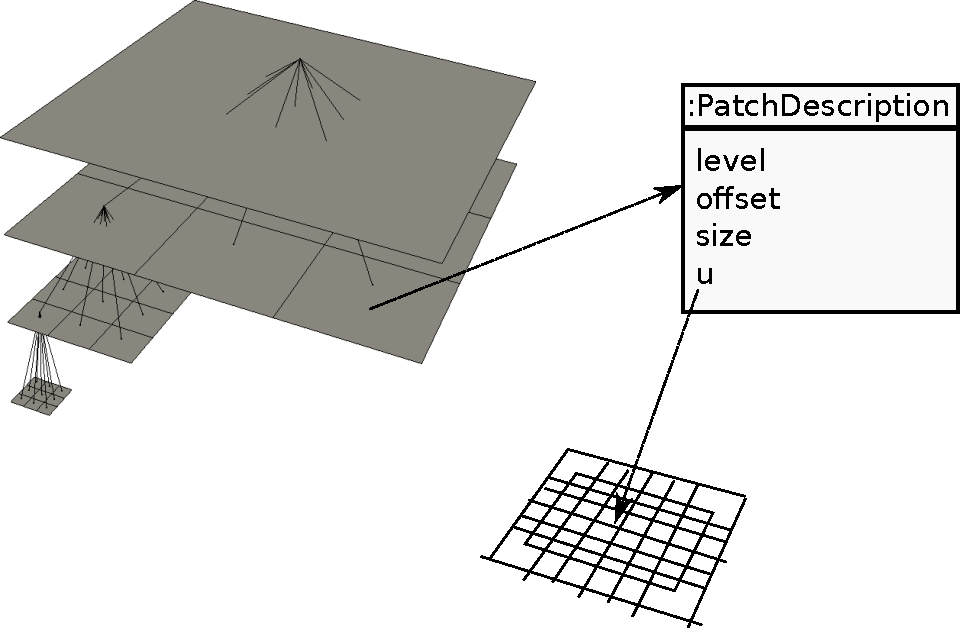
\includegraphics[width=0.5\textwidth]{44_patch-based-solver/data.pdf}
\end{center}

\noindent
It is up to you to specificy the semantics of the data arrays used. 
They can represent overlapping or non-overlapping patches.
It just has paid off not to make any overlap exceed any neighbouring cell on the
same level.
The introductory sketch of this chapter illustrates $4\times 4$ patches with a
ghost layer/overlap of one. 
A code for this setup might read as follows:

\begin{code}
void myprojectsnamespace::Cell::initCellInComputeTree( ... ) {
  const int numberOfPatchDescriptionsPerCell = 1;
  const int newPatchIndex = PatchDescriptionHeap::getInstance().createData
    (numberOfPatchDescriptionsPerCell);
  _cellData.setPatchIndex( newPatchIndex );
  assertion( newPatchIndex>=0 );

  records::PatchDescription&  patchDescription =
    PatchDescriptionHeap::getInstance().getData(newPatchIndex)[0]; 
  
  patchDescription.setU( DataHeap::getInstance().createData(7*7) );
  patchDescription.setLevel(...);
  patchDescription.setOffset(...);
  patchDescription.setSize(...);
}

\end{code}


\begin{remark}
  There is absolutely no reason to restrict a code to use only the finest level
  of the spacetree. Furthermore, it might make sense to use different patch
  sizes in different cells of the same level. Please note that all the patch
  techniques also work if you store higher order DG shape functions in your
  cells, e.g.
\end{remark}



\subsection{Working with patches on regular grids}

As each cell points to patch description through its field \texttt{PatchIndex},
it is a natural choice to work with the associated patch data in
\texttt{enterCell}.
Before we actually do the work, we use the data from the 
\texttt{PatchIndex} objects of the neighbouring cells to initialise our ghost
cells.
In our case, a simple copying does the job. In other situations, you might have
to implement more sophisticated projection operators.

\begin{code}
#include "multiscalelinkedcell/HangingVertexBookkeeper.h"
#include "multiscalelinkedcell/SAMRTools.h"
#include "peano/utils/Loop.h"
...
void pesplines::mappings::JacobiUpdate::enterCell( ... ) {
 if (
  !fineGridCell.isRefined()
  &&
  multiscalelinkedcell::HangingVertexBookkeeper::allAdjacencyInformationIsAvailable(
   VertexOperations::readPatchIndex(fineGridVerticesEnumerator,fineGridVertices)
  )
 ) {
  intialiseGhostLayerOfPatch(
    fineGridCell,
    fineGridVertices,
    fineGridVerticesEnumerator
  );
   
  solve(
    PatchDescriptionHeap::getInstance().getData( fineGridCell.getPatchIndex() )[0],
    fineGridVerticesEnumerator.getCellSize()
  );
 }  
}
\end{code}

\noindent
The use of the predicate \texttt{allAdjacencyInformationIsAvailable} is too
careful here: it should always return \texttt{true}.
In dynamically adaptive settings, it can happen that adjacency information in
the vertices (i.e.~which patch descriptions are held by the adjacent cells) it
not up-to-date immediately.
In such a case, the branching would skip a cell with incomplete data and wait
for the next traversal where all information is available.


The initialisation of the ghost layer uses Peano's d-dimensional loops (the
code then should work for $d=3$ as well), it rather technical, but not too
difficult to understand as it realises plain copying at the end of the day.
Again, we use operations provided by the \texttt{multiscalelinkedcell} package:

\begin{code}
void pesplines::mappings::MatVec::intialiseGhostLayerOfCell(
 Cell&                                 fineGridCell,
 Vertex * const                        fineGridVertices,
 const peano::grid::VertexEnumerator&  fineGridVerticesEnumerator
) {
 const tarch::la::Vector<THREE_POWER_D,int> neighbourCellIndices = 
  multiscalelinkedcell::getIndicesAroundCell(
   VertexOperations::readPatchIndex(fineGridVerticesEnumerator,fineGridVertices)
 );

 assertion3(
   multiscalelinkedcell::HangingVertexBookkeeper::allAdjacencyInformationIsAvailable(
    VertexOperations::readPatchIndex(fineGridVerticesEnumerator,fineGridVertices)
   ),
   fineGridVerticesEnumerator.toString(),
   VertexOperations::readPatchIndex(fineGridVerticesEnumerator,fineGridVertices),
   neighbourCellIndices
 ); // no enty of neighbourCellIndices points to a patch description on the
    // heap that does not exist
 
 // we take data from surrounding patches and always write into the
 // patch in the center (destPatchDescription)
 records::PatchDescription& destPatchDescription = 
  PatchDescriptionHeap::getInstance().getData( fineGridCell.getPatchIndex())[0];

 dfor3(i)
  // i does not point to the central patch (all entries 1) and is valid
  // i.e. we are not at the domain boundary, e.g.
  if (
   i!=tarch::la::Vector<DIMENSIONS,int>(1) &&
   neighbourCellIndices(iScalar) > 
    multiscalelinkedcell::HangingVertexBookkeeper::InvalidAdjacencyIndex
  ) {
   assertion(neighbourCellIndices(iScalar)>=0);
   records::PatchDescription& srcPatchDescription 
    = PatchDescriptionHeap::getInstance().getData( neighbourCellIndices(iScalar) )[0];
 
   // this if is always true as long as we work with a regular grid
   if (srcPatchDescription.getLevel()==destPatchDescription.getLevel()) {
    // so now write your well-suited for loop here that befill all entries 
    // of the ghost layer of your patch. If the for loop determines the 
    // indices destVertexIndex and srcVertexIndex specifying vertices within 
    // the patch, then the loop body copying the data around reads as 
    DataHeap::getInstance().getData(destPatchDescription.getU())
      [destVertexIndex]._persistentRecords._u =
     DataHeap::getInstance().getData(srcPatchDescription.getU())
      [srcVertexIndex]._persistentRecords._u;
   }
  }
 enddforx // counterpart of dfor3 (see documentation in source code)
}
\end{code}

\noindent
The texttt{dfor3(i)} runs over a $\{0,1,2\}^d$ domain.
In the loop body (that has to be terminated by a \texttt{enddforx} pragma), it
provides two loop counters: \texttt{i} is a d-dimensional integer vector where
each entry is from $\{0,1,2\}$.
Furthermore, it gives us another loop counter \texttt{iScalar} which runs from 0
through $3^d-1$, i.e.~is a linearisation of \texttt{i}.
All the macros are defined in \texttt{Loop.h}.


\texttt{getIndicesAroundCell} is a helper function that takes the $2^d$ adjacent
vertices of a cell.
It actually requires their \texttt{PatchIndex} entries which are automatically
set by the predefined mapping.
The helper tool returns an array with $3^d$ entries to be read as a $3^d$
integer field.
The first entry holds the patch index of the left bottom neighbour.
The second entry holds the patch index of the bottom neighbour.
The fourth entry holds the patch index of the left neighbour.
The fifth entry hold the patch index of the cell itself.
And so forth.
The operation works for any dimension.
Study its source code documentation for details.


How the actual copying is done depends on the semantics of your data. 
It also depends on column-major or row-major storage formats for the patch data.
The implementation of the actual \texttt{solve} operation then finally is
straightforward: take the $u$-array and run through it. Again, a \texttt{dfor}
loop might simplify your code.
If you struggle with the \texttt{solve} operation, it might make sense to study
the plotting in the next section first. 
It uses exactly the sketched loop of the patch entries.


\begin{remark}
  It is not clear a priori whether it is better to have overlapping patches or
  non-overlapping data structures. With overlaps, there's an additional memory
  overhead for redundant data and data has to be moved around in the preamble of
  \texttt{enterCell}, e.g. In return, the actual work on the patches can be
  realised on a continuous array; and thus benefit from vectorisation and
  parallel fors. Alternatively, one can not use any redundant data and instead
  access the neighbouring data indirectly. This makes the actual computation
  often more complicated (one has to analyse whether data is held within the
  patch of comes from an adjacent patch), but induces no memory overhead and
  perhaps reduces the stress on the memory subsystem.
\end{remark}



\subsection{Plotting}

We briefly sketch what rapid coding of the plotting of a patch-based solver
might look like.
For this, we rely on a mapping \texttt{Plot} that holds plotter classes from 
Peano's plotter component.


\begin{code}
#include "tarch/plotter/griddata/blockstructured/PatchWriterUnstructured.h"

namespace pesplines {
  namespace mappings {
    class Plot;
  }
}

class pesplines::mappings::Plot {
  private:
    ...
    static int                  _snapshotCounter;

    tarch::plotter::griddata::blockstructured::PatchWriter*                      _writer;
    tarch::plotter::griddata::blockstructured::PatchWriter::SinglePatchWriter*   _patchWriter;
    tarch::plotter::griddata::blockstructured::PatchWriter::VertexDataWriter*    _uWriter;
};
\end{code}

\noindent
The implementation plugs into \texttt{beginIteration} and \texttt{endIteration}
to open the plotter or to write its data into a file, respectively.
Depending on the build type, we either plot binary data or we plot a plain text
file that is easier to debug.

\begin{code}
int ...::mappings::Plot::_snapshotCounter(0);

void ...::mappings::Plot::beginIteration(
  ...::State&  solverState
) {
  #if defined(Asserts) || defined(Debug)
  _writer = new tarch::plotter::griddata::blockstructured::PatchWriterUnstructured( 
    new tarch::plotter::griddata::unstructured::vtk::VTKTextFileWriter() );
  #else
  _writer = new tarch::plotter::griddata::blockstructured::PatchWriterUnstructured( 
    new tarch::plotter::griddata::unstructured::vtk::VTKBinaryFileWriter() );
  #endif
  _patchWriter            = _writer->createSinglePatchWriter();

  _uWriter         = _writer->createVertexDataWriter("u",3);
}


void ...::mappings::Plot::endIteration(
  ...::State&  solverState
) {
  _patchWriter->close();
  _uWriter->close();

  delete _uWriter;
  delete _patchWriter;

  _uWriter = 0;
  _patchWriter = 0;

  std::ostringstream snapshotFileName;
  snapshotFileName << "solution"
                   #ifdef Parallel
                   << "-rank-" << tarch::parallel::Node::getInstance().getRank()
                   #endif
                   << "-" << _snapshotCounter
                   << ".vtk";
  _writer->writeToFile( snapshotFileName.str() );

  _snapshotCounter++;

  delete _writer;
  _writer = 0;
}
\end{code}

\noindent
The heart of the plotting can be found in \texttt{enterCell} where the
actual patch data it piped into the solution plotter:


\begin{code}
void ...::mappings::Plot::leaveCell(...) {
 if ( !fineGridCell.isRefined() ) {
  assertion(PatchDescriptionHeap::getInstance().isValidIndex(fineGridCell.getPatchIndex()));
  const records::PatchDescription& patchDescription   
   = PatchDescriptionHeap::getInstance().getData( fineGridCell.getPatchIndex() )[0];

  const std::pair<int,int> indexPair = _patchWriter->plotPatch(
    fineGridVerticesEnumerator.getVertexPosition(),
    fineGridVerticesEnumerator.getCellSize(),
    4+1 // number of inner cells per spacetree leaf
  );

  int unknownVertexIndex = indexPair.first;
  //int unknownCellIndex   = indexPair.second;

  dfor(i,4+1) {
   const tarch::la::Vector<DIMENSIONS,int> currentVertex = i + 1;
   const int linearisedCurrentVertex 
    = peano::utils::dLinearisedWithoutLookup(currentVertex,4+1);
   const double u = DataHeap::getInstance().getData(patchDescription.getU())
    [linearisedCurrentVertex]._persistentRecords._u;

    _uWriter->plotVertex( unknownVertexIndex,u );
    unknownVertexIndex++;
  }
 }
}
\end{code}



\subsection{Adaptive grids}

We do not detail the handling of adaptivity with patches here. 
However, the basic principle is extremely simple: 
The toolbox's reconstruction algorithm is completely equipped to handle
resolution changes, i.e.~if a left neighbour resides of a cell resides on a
coarser level, the correct index is written into the left neighbour.

This implies that
\begin{enumerate}
  \item Several neighbour indices might be equal if neighbours reside on coarser
  levels.
  \item Fine grid cells always can read and write data from coarser adjacent
  cells.
  \item Fine to coarse information however also can be transported within the
  tree as any cell has at some stages access to its parent.
\end{enumerate}

\begin{remark}
Peano does not enforce any 2:1 balancing on the grid. However, such a balancing
might be desireable from an application point of view. You can either program
some balancing on your own, or you can merge the predefined mapping
\texttt{GridBalancer2to1} into your adapters.
\end{remark}




\subsection*{Further reading}

\begin{itemize}
  \item   Unterweger, K., Wittmann, R., Neumann, P., Weinzierl, T. and Bungartz,
  H.-J.
(2015), {\em Integration of FULLSWOF2D and PeanoClaw: Adaptivity and Local
Time-stepping for Complex Overland Flows}, in Mehl, M., Bischoff, M. & Schäfer,
M. eds, Lecture notes in computational science and engineering, 105 Part II: 3rd International Workshop on Computational Engineering CE 2014. Stuttgart, Germany, Springer, 181-195.
\item Weinzierl, Tobias, Wittmann, Roland, Unterweger, Kristof, Bader, Michael,
Breuer, Alexander and Rettenberger, Sebastian (2014), {\em Hardware-aware block
size tailoring on adaptive spacetree grids for shallow water waves}, in
Gr\"o\ss linger, Armin and K\"ostler, Harald eds, HiPEAC HiStencils 2014 - 1st
International Workshop on High-Performance Stencil Computations. Vienna, Austria.
\item Weinzierl, Tobias, Bader, Michael, Unterweger, Kristof and Wittmann,
Roland (2014). {\em Block Fusion on Dynamically Adaptive Spacetree Grids for
Shallow Water Waves}. Parallel Processing Letters 24(3): 1441006.
\end{itemize}




%  % Patch-based shallow water
%  % MD oder irgendwas body-maessiges
% 
% 
%  
%  \chapter{Parallel Computing}
%   \label{chapter:parallel}
%   \section{Shared memory parallelisation}
  \label{section:parallelisation:shared-memory}


\chapterDescription
  {
    30 minutes.
  }
  {
    A working simulation code and a compiler that supports either OpenMP or
    Intel's Threading Building Blocks (TBB) \footnote{At the moment, Peano's
    OpenMP support is slightly outdated. All examples should work straightforwardly
    with TBB however.}.
  }

In this section, we discuss how to parallelise a simulation code on a shared
memory architecture.
Hereby, we focus on Peano's parallelisation features. 
In mature, big applications, they are typically supplemented by further
parallelisation that is application-specific: Peano can run lots of routines in
parallel if it is correctly used. 
This way, we are able to exploit several cores.
To exploit modern multicore and manycore architectures, codes however also have
to use parallelised routines, linear algebra, and so forth.
This is an additional level of parallelism that cannot be tackled here.

\subsection{Preparation}
\label{section:shared-memory:preparation}

Peano compiles in parallel out-of-the-box if you use the PDT to setup a project
blueprint. 
To facilitate a shared memory parallel build, you have to translate your code
with the compile flag \texttt{-DSharedTBB}. 
Alternative variants are \texttt{-DSharedOMP}, e.g.
Once you edit your makefile and add this compile flag, please also provide the
correct include and link paths to the makefile.
For modern Intel compilers, no changes should be required, as Intel's TBB come
along with the compiler suite.

By default, the auto-generated \texttt{main} configures the parallel environment. 
While OpenMP relies on the setup of a well-suited thread count via environment
variables, TBB requires/allows the user to select a thread count manually. 
If you want to configure the thread count this way, please add the corresponding
instructions to your \texttt{main}.
To make your code portable (and to preserve a serial version), I recommend to
embed all shared memory-specific routines into ifdefs.
Besides the aforementioned \texttt{SharedXXX} defines, Peano also provides a
flag \texttt{SharedMemoryParallelisation} that is set as soon as OpenMP or TBB
is selected.
To make use of it, you have to include
\linebreak \texttt{MulticoreDefinitions.h}.

\begin{code}
#ifdef SharedMemoryParallelisation
#include "tarch/multicore/Core.h"
#endif

#include "tarch/multicore/MulticoreDefinitions.h"

  // should be generated by the PDT
  int sharedMemorySetup = peano::initSharedMemoryEnvironment();
  ...


  // manual configuration of threads (optional)
  #ifdef SharedMemoryParallelisation
  const int         numberOfCores    = 16;
  tarch::multicore::Core::getInstance().configure(numberOfCores);
  #endif

\end{code}

\noindent
Peano's kernel uses multiple threads in several places. 
However, most of these concurrent fragments are really very short-running.
As a result, it is not clear whether it pays off to use multithreading or not.
Therefore Peano uses an oracle---an object that returns per grid
traversal phase whether multitasking should be used or not.
This oracle can be found in \linebreak
\texttt{peano/datatraversal/autotuning}\footnote{The namespace choice
\texttt{autotuning} is wrong. The namespace collects classes that allow you to
tailor your shared memory parallelisation. Our original design intention has
always been to work with autotuning to get rid of as many parameters as
possible. That's where the namespace identifier comes from.}.
Details on this oracle are discussed later.
For the time being, insert a commands into your runner.

\begin{code}
int mynamespace::runners::Runner::run() {
  #ifdef SharedMemoryParallelisation
  peano::datatraversal::autotuning::Oracle::getInstance().setOracle(
    new peano::datatraversal::autotuning::OracleForOnePhaseDummy(true)
  );
  #endif
  ...
}
\end{code}

\noindent
The \texttt{true} parameters enables multicore support.
It might be reasonable to study the other parameters (see either the header
file or Peano's webpages) later.
Right now, it should be possible to recompile the code and to run a first
version on a shared memory machine.
It probably won't yield that much parallel speedup though \ldots


\subsection{Specifying concurrency levels}

Peano's fundamental idea is that users use events to say what is to be done. 
But codes leave it to the kernel to decide when and---anticipating some
constraints---in which order it is done.
This property is exploited by the multicore variant: 
Peano mappings specify whether multiple calls to one event (such as
\texttt{enterCell}) may run in parallel.
The kernel then decides autonomously whether to run in parallel and on which
cores.


To make this work, we have to revise the concept of an adapter. 
An adapter invokes multiple events.
Therefore, the concurrency level of an event has to be the most pessimistic
combination of the concurrency levels of all mappings realising this event.
This combination is automatically determined by the adapters generated by the
PDT.


Concurrency levels are specified within the events. 
Per event there is one concurrency specification. 
\texttt{touchVertexFirstTime}'s concurrency level for example is specified by
the routine \linebreak
\texttt{touchVertexFirstTimeSpecification}.
If you want to run \texttt{touchVertexFirstTime} in parallel, open all mappings
and edit \texttt{touchVertexFirstTimeSpecification} in each individual one.


A specification returns an instance of \texttt{peano::MappingSpecification}. 
Such an instance accepts parameters:
\begin{itemize}
  \item The first flag specifies whether the corresponding event works on the
  whole tree, only on its leaves, or whether it actually does not implement
  anything at all.
  \item The second flag specifies whether a particular event may run in
  parallel.
  \item The third flag specify whether a particular event modifies the mapping's
  state itself. It basically means whether the event can be considered by Peano
  as \texttt{const}. If an event does not change the mapping's state, we
  obviously can parallelise more aggressively and do not have to merge back any
  changes in the mapping with \texttt{mergeWithWorkerThread}.
  \item Further flags specify whether events support resiliency and other
  experimental features. For most Peano kernel variants, such further flags are
  not supported. We maintain these variants in experimental Peano kernels only.
\end{itemize}

\begin{remark}
Even if you run your code without any shared memory parallelisation, it makes
sense to tailor all specifications. If your code does work on the finest tree
levels only, e.g., you can obtain significant speedup if you change the
\texttt{WholeTree} flag into \texttt{OnlyLeaves}. The most significant (serial)
speedups are obtained if you mark all specs as \texttt{Nop} where the actual
mapping does not do anything in the corresponding events. In this case, the
Peano kernel can skip whole function calls completely.
\end{remark}

\begin{remark}
If you tune/parallelise particular events and if you, at the same time, use
predefined mappings, you may have to study the specification objects
constructed there. Adapters always have to work pessimistically. If a predefined
mapping requires a particular event to be called sequentially (for plotters,
e.g.), you can specify any concurrency level you want---the kernel always will
run the whole event serially.
\end{remark}


For a quick start, I recommend to pick one particular event that is not
empty and where you do know exactly that it can run in parallel with other
events.
Select the correct concurrency level then:
\begin{itemize}
  \item Serial specifies that this event may not run in parallel and
  \item All other variants allow the kernel to issue events in parallel.
  However, they anticipate certain data dependencies---you may for example
  decide that entering a cell may be issued in parallel as long as no two events
  can access two adjacent vertices at the same time. This way, you anticipate
  data races.
\end{itemize}



\subsection{Ensuring inter-thread data consistency}

Once a parallel event is identified, the Peano kernel may run it on multiple
threads in parallel.
For this, the whole mapping object is replicated. 
The replication triggers the mapping's copy constructor.
Once the parallel phase is processed---all cells have been entered in parallel,
e.g.---all mapping replica are destroyed again and merged into one mapping that
is held by the adapter.
The mappings provide routines to plug into this life cycle.

In the copy constructor, you have to copy all mapping attributes that you need
in your parallel routines.
Two scenarios appear most often: Globally read properties such as a state object
are copied to each thread instance of the mapping.
Globally written attributes such as a global residual are set to zero in the
copy constructor:

\begin{code}
#if defined(SharedMemoryParallelisation)
mynamespace::MyMapping::MyMapping(const Collision&  masterThread):
  _localState( masterThread._localState ) {
  // alternatively, we could call
  // _localState = masterThread._localState;
  
  // now we clear all reduced/accumulated data:
  _localState.clearAttributes();
}
\end{code}

\noindent
The counterpart of the copy constructor is the routine
\texttt{mergeWithWorkerThread} that is invoked every time a mapping has been
replicated to run in parallel on multiple cores and this parallel phase is about
to terminate.
Peano does not use the destructor of the mapping to merge data to obtain a finer
control of thread replica and to be able to reuse mapping instances.

Usually, the merger only reduces globally accumulated data in this routine. 
If you have followed the recommendation in Section
\ref{section:applications:heat-equation} to make mappings hold copies of the
\texttt{State} object and to offer a merge routine, the mapping's shared
memory code resembles

\begin{code}
void mynamespace::MyMapping::::mergeWithWorkerThread(
  const mynamespace::MyMapping& workerThread
) {
  logTraceIn( "mergeWithWorkerThread(Collision)" );

  _localState.merge( workerThread._localState );
  
  logTraceOut( "mergeWithWorkerThread(Collision)" );
}
#endif

\end{code}


\subsection{Tailoring the oracle}

The oracle is the central point of control to decide whether event should be
invoked in parallel for given problem sizes.
The mapping specifications decide whether events may run in parallel.
The oracle specifies whether concurrent events should run in parallel for a
given problem size.


Whenever the kernel runs into a particular set of events and decides that it
would like to invoke those events in parallel, it realises the following
workflow:
\begin{itemize}
  \item Ask the adapter whether its combination of events allows the kernel to
  run events in parallel. If the result is a yes:
  \item Tell the oracle which adapter currently is active.
  \item Pass the oracle the problem size and ask which grain size (minimal
  problem chunk size) might be used. 
  \item If the adapter returns 0, nothing is ran in parallel. 0 should be
  returned by the oracle if the problem overall is too small to benefit from any
  shared memory parallelisation.
  \item Otherwise, split the problem into sizes of size at least grain size,
  replicate the mapping as often as required, and start using multiple threads.
\end{itemize}

\begin{remark}
 To make Peano as lightweight as possible, it internally works with static
 partitioning only. Features such as dynamic subpartitioning of problems are
 switched off. This lightweight approach in turn means that choosing a proper
 grain size for each and every step  is important. The oracles allow you to make
 exactly this choice.
\end{remark}


\noindent
As clarified, each adapter is associated to one oracle, i.e.~you are able to
use oracles specifying grain and minimal problem sizes on a per-adapter base.
Furthermore, oracles are not static.
They have a state and thus can for example `learn' which grain sizes are
reasonable (cmp.~paper by Nogina et al.).
For a quick start, trial and error with
\texttt{peano::datatraversal::autotuning::}
\texttt{OracleForOnePhaseDummy} is usually sufficient: 
Here you can hardcode grain sizes via the oracle's constructor.
Just modify some of the default values and study how the actual CPU usage
and the time-to-solution change.
Once you have detailed knowledge about your application's behaviour, it might
be reasonable to replace the Dummy with a tailored implementation of
\texttt{peano::datatraversal::autotuning::OracleForOnePhase}.


Peano's homepage offers a few more sophisticated oracles. 
Notably, there is one oracle that samples all different types of grain sizes and
one oracle that does real-time measurements to ``learn'' what good grain sizes
look like. 
These oracles come along with some Phyton scripts that allows users to analyse
their insights graphically or as tables.
See the class documentations.


Important for all sophisticated oracles is that they give the user the
opportunity to plot their statistics within the runner. 
To obtain these statistics, call
\begin{code}
  peano::datatraversal::autotuning::Oracle::getInstance().plotStatistics( "" );
\end{code}
The routine expects an filename.
If none is given, i.e.~you pass the empty string, all output is written to the
terminal.
Many oracles also provide routines to reload these statistics.
This way, statistical data is not always created from scratch but incrementally
updated.


\begin{remark}
 Under the umbrella of the ExaHyPE project, Peano's autotuning oracle named
 \texttt{OracleForOnePhaseWithShrinkingGrainSize} saw some significant
 improvement. It uses real-time measurements to identify good grain sizes. 
 If real-time measurements are supported on your system---we faced some issues
 on KNL systems where the timers seem to give imprecise answers---then this
 oracle usually does a good job. While the oracle realises ideas published in
 the paper by Nogina et al.~it saw some significant improvements since the
 publication. Please consult the extensive class documentation in the header for
 details.
\end{remark}



\subsection{Working with Peano's tasks, semaphores, locks and loops}

All shared memory parallelisation standards today provide tasks, semaphores,
locks, and so forth.
Peano provides a wrapper around those which allows you to create one
implementation that then runs with OpenMP, TBBs and so forth.
To use them, I recommend to study all classes stored in
\texttt{tarch::multicore}.
Notably \texttt{BooleanSemaphore} and \texttt{Lock} are of interest:

\begin{code}
  static tarch::multicore::BooleanSemaphore  mysemaphore;
  
  
  tarch::multicore::Lock   myLock(mysemaphore);
  
  ...            // critical section
  
  myLock.free(); // destructor would free semaphore automatically
\end{code}


\noindent
The code above is removed automatically if you do not use OpenMP or TBB.
Otherwise, it introduces a critical section that is processed by at most one
thread at a time.

Furthermore, the header \texttt{Loop.h} might be of interest. 
It provides very useful macros:
\begin{itemize}
  \item \texttt{pfor} is a macro resembling a simple for-loop. If you compile
  your code with any shared memory compile flag, it makes the loop run in
  parallel.
  \item \texttt{pdfor} is a \texttt{pfor} as well. However, it does not traverse
  a linear sequence but runs over a $d$-dimensional index set. Very useful
  within a cell, e.g., where you have to do something with all vertices, while
  all vertices can be processed in parallel.
\end{itemize}


Peano's task concept basically mirrors TBB's task concept. 
However, if you implement everything within Peano's context, you can also switch
to OpenMP later on.
The idea is very simple: You create a new class that does you job and
you create an instance of this class in your code.
Ensure that the class has a functor:

\begin{code}
  void MyTaskClass::operator()() {
   ...   // do whatever you wanna do in your task 
  } 
\end{code}

\noindent
and then pass it over to the \texttt{TaskSet} class:

\begin{code}
  MyTaskClass myTask(...); // pass in the constructor whatever dataa your task needs 
  peano::datatraversal::TaskSet( myTask ); // the task now runs in the background
\end{code}

\noindent
This constructor sends \texttt{myTask} to the background and continues. 
It does not wait for the task to finish.
A classic pattern is that you introduce a boolean set to false before you launch
the task.
Modifications to the boolean are protected by a semaphore.
Once the task's \texttt{operator()} function finishes, it sets the bool.
The main thread meanwhile continues, but then there's a while loop that
continues to poll the boolean

\begin{code}
  bool terminated = false;
  while (!terminated) {
    tarch::multicore::Lock myLock( _myStaticSemphore );
    terminated = _myGlobalBool;
  }
\end{code}

\noindent
until it is set.

Finally, there are two useful static operations in \texttt{BooleanSemaphore}.
The operation \linebreak
\texttt{tarch::multicore::BooleanSemaphore::sendTaskToBack()}
which is useful to realise \linebreak low-\-priority tasks: Other tasks in the
system (see section below) are activated if you call this operation.


Please note that there are other constructors of \texttt{TaskSet} that run
multiple tasks in parallel and wait until both have terminated. 
See the class description for details.



\subsection{Profiling}

Peano provides some tailored, built-in profiling for shared memory codes. 
See the Section \ref{section:performance-analysis} for some details on this. 
The idea is that you recompile your code with an additional flag.
This gives you some output (pipe it into a file), and then there is a Python
script in the directory \texttt{peano/performanceanalysis} that allows you to
create a HTML page from this output that comprises lots of performance analysis
graphs and gives you hints where your CPUh are burnt. Obviously, this approach
is problematic for large runs producing lots of data, and it also suffers from
quite an overhead polluting your actual results.

If you want to use Intel's VTune Amplifier, we see many analyses be polluted,
too, as we use tons of templates, tons of inlinings consequently, and thus mess
up many profiles. To get more verbose outputs with the correct meta data, please
recompile your code with \texttt{-debug inline-debug-info}.


\subsection*{Further reading}

\begin{itemize}
  \item Weinzierl, Tobias, Bader, Michael, Unterweger, Kristof and Wittmann,
  Roland (2014). {\em Block Fusion on Dynamically Adaptive Spacetree Grids for
  Shallow Water Waves}. Parallel Processing Letters 24(3): 1441006.
  \item Schreiber, Martin, Weinzierl, Tobias and Bungartz, Hans-Joachim (2013).
  {\em Cluster Optimization and Parallelization of Simulations with Dynamically
  Adaptive Grids}. Euro-Par 2013, Berlin Heidelberg, Springer-Verlag.
  \item Schreiber, Martin, Weinzierl, Tobias and Bungartz, Hans-Joachim (2013).
  {\em SFC-based Communication Metadata Encoding for Adaptive Mesh}. Proceedings
  of the International Conference on Parallel Computing (ParCo), IOS Press.
  \item Nogina, Svetlana, Unterweger, Kristof and Weinzierl, Tobias (2012).
  {\em Autotuning of Adaptive Mesh Refinement PDE Solvers on Shared Memory
  Architectures}. PPAM 2011, Heidelberg, Berlin, Springer-Verlag.
  \item Eckhardt, Wolfgang and Weinzierl, Tobias (2010). {\em A Blocking
  Strategy on Multicore Architectures for Dynamically Adaptive PDE Solvers}.
  Parallel Processing and Applied Mathematics, PPAM 2009, Springer-Verlag.
\end{itemize}

%   
%   \newpage
%   \section{MPI parallelisation}
  \label{section:parallelisation:mpi}


\chapterDescription
  {
    180 minutes.
  }
  {
    A working simulation code and working MPI environment.
  }

In this section, we discuss how to parallelise a simulation code with message
passing.

\subsection{Preparation}

Peano technically relies on MPI with its SPMD paradigm, i.e.~all ranks run
exactly the same code.
Internally, it however creates a logical tree topology on all ranks and
reserves one rank for non-compute tasks.
This one is called the {\em global master}.
By convention, this is rank 0, i.e.~the very first rank launched by MPI.
All other ranks are {\em workers}.
Each rank besides the global master has one unique {\em master}.
Each worker can either be active, i.e.~participate in the computation, or it can
be idle.
At the begin of the simulation, all workers are idle and only the global master
is working (as it is working always).

The global master usually has exactly one worker rank to which it delegates all
compute work and which in turn continues to distribute work recursively.
The global master thus ``only'' remains in control of the algorithm control,
load balancing decisions, administrative tasks, \ldots
Those are typically time critical and it thus seemed to be reasonable to free
the global master from compute work.
Whenever the global master triggers a grid traversal, it tells all non-idle
workers which adapter is currently used.
It determines which algorithmic phase to run. 
Then, it starts to run through the grid. 
If parts of the grid are deployed to other ranks---as clarified, the global
master always deploys the coarsest spacetree cell plus all of its children to a
worker immediately---they are informed to start a traversal as well.
The traversal kick-off propagates through the ranks along the master-worker
topology.
All of this is done automatically.
Most codes require the programmer to think only about the global master.

\paragraph{Re-translating the code}
We expect that there is a command \texttt{mpicxx} available in your path.
This command often also is called \texttt{mpiCC}. Please ensure it calls the
right compiler backend. 
If you are unsure, check with argument \texttt{-V} and adopt the backend
manually if required. 

Change your compile command to \texttt{mpicxx} and add the two options
\begin{code}
  -DParallel -DMPICH_IGNORE_CXX_SEEK
\end{code}
to your compiler call.
While Peano is written in C++11, it relies only on C bindings of MPI.
Some MPI versions (mpich, e.g.) have/used to have issues with this combination
(give you tons of warnings) unless you pass \texttt{MPICH\_IGNORE\_CXX\_SEEK}. 


\paragraph{Setting up the code}

The auto-generated \texttt{main} calls Peano's operation \newline
\texttt{peano::initParallelEnvironment} which takes care of a proper MPI
initialisation. 
As soon as the initialisation has terminated without an error code, you may use
the predicate

\begin{code}
if (tarch::parallel::Node::getInstance().isGlobalMaster()) {
  ...
}
\end{code}

\noindent
to find out whether a particular piece of code runs on the global master. 
One of the first steps in many codes might be to perform some tests only on this
global master.
The counterpart \linebreak
\texttt{peano::shutdownParallelEnvironment()} typically is
invoked directly within \texttt{main} as well and is also called by the
autogenerated templates already.

As we follow SPMD, \texttt{main} has to create an instance of the runner and
invoke its \texttt{run} operation. 
The \texttt{run} then distinguishes between the global master and all the other
workers that blindfolded follow their masters. 
\begin{code}
  int result = 0;
  if (tarch::parallel::Node::getInstance().isGlobalMaster()) {
    result = runAsMaster( *repository );
  }
  #ifdef Parallel
  else {
    result = runAsWorker( *repository );
  }
  ...
\end{code}

\noindent
This code is generated and it is most of the time sufficient to focus on the
operation \texttt{runAsMaster}, i.e.~to focus on the serial code version. There
are however a few steps that have to be done on each individual worker
separately. 
You may implement this within the \texttt{main}.
However, we typically realise it within \texttt{run} just before or after the
operation splits up into the function for the global master and all other ranks.


\paragraph{Choose a load balancing request answering strategy on the global
master}
One for the first steps on the global master is to configure a
proper load balancing strategy. 
Peano realises a hybrid centralised-decentralised load balancing by default,
where load balancing decisions are, whenever possible, made decentrally,
i.e.~on the individual ranks.
Once load balancing decisions are made (along the lines `I would like more
ranks to help me with my work'), a central point is contacted that decides which
ranks are involved in the rebalancing.
This central point is called {\em node pool}; 
and it is instantiated on the global master which is typically rank 0.
We see why it is important to free the global master from work: if a rank wants
to do some load balancing and needs both permissions to do so and potentially
involved nodes, it pauses its traversal and asks the node pool.
So it is essential that the answer arrives as soon as possible.


Peano realises the whole node pool itself, no coding is required here, but
it allows the user to plug into the decisions which ranks are assigned to assist
other rankOracleForOnePhaseWithGreedyPartitionings, e.g.
We hence have to configure the node pool on the global master only
\begin{code}
if (tarch::parallel::Node::getInstance().isGlobalMaster()) {
  tarch::parallel::NodePool::getInstance().setStrategy(
    new tarch::parallel::FCFSNodePoolStrategy()
  );
}
\end{code}

\noindent
where we select here one of the default strategies. 
It answers to any incoming load balancing request FCFS (while other strategies
might decide to bundle requests to get an overview who asks for resources first
before any rank assignment is performed) and hands out MPI ranks as long as
there are still idle workers available.


\begin{remark}
 All classes from the \texttt{tarch::parallel} namespace and the
 \texttt{peano:parallel} namespace can be included even if you work without
 distributed memory parallelisation or want your code to be prepared to compile without MPI, too.
 Notably, the classes \texttt{Node} and \texttt{NodePool} all implement their
 routines for serial setups as well.
\end{remark}


\paragraph{Restart the load balancing on all ranks}
Once the node pool
is initialised, we have to restart it.
This has to be done on all ranks. 
On the global master, the operation really restarts the node pool.
On all other ranks, it establishes the connection to the central node pool
and informs the latter how many ranks are available.

\begin{code}
tarch::parallel::NodePool::getInstance().restart();
tarch::parallel::NodePool::getInstance().waitForAllNodesToBecomeIdle();
\end{code}

\begin{remark}
Many sophisticated load balancing schemes can deal with MPI ranks signing in and
out throughout the computation dynamically.
Peano per se can deal with dynamic rank allocation.  
However, the default FCFS strategy is not that elaborate. 
It requires that all ranks are well-known when it starts up and that they do not
change.
Therefore, it is mandatory to add the \texttt{waitForAllNodesToBecomeIdle()}
instruction here which ensures that all nodes register at the central node pool
and tell the central node pool strategy that they are idle and free for new
jobs. 
Though not mandatory, you might want to add this statement anyway at runtime to
ensure your whole system is up properly before any load balancing kicks in.
\end{remark}

\paragraph{Configure the load balancing strategy on all ranks}
In a next step, we configure the
actual load balancing.
So far, only the global master is established that can decide which ranks
collaborate.
We still need to establish the environment that first decides per rank whether
to load balance or not.
Again, we rely on a default balancing that simply yields
a static partitioning.
The partitioning, i.e.~the domain splitting, is determined by a greedy grid
decomposition.
Following our description, this setup has to run on each and every rank.

\begin{code}
peano::parallel::loadbalancing::Oracle::getInstance().setOracle(
 new peano::parallel::loadbalancing::OracleForOnePhaseWithGreedyPartitioning(false)
 );
\end{code}

\noindent
This trivial load balancing runs embarrassingly parallel on all ranks. 
The \texttt{false} switches off joins, i.e.~we decompose the grid in a greedy
fashion.

Peano's general idea is the these oracles implement the load balancing and you
can create your own oracle tailored to your needs if you wish.
There are also some default oracles available from the homepage (though not
included in the kernel---the above one is the only one in the kernel to allow
you a quick start) that might suit you.
In principle, you could use different oracles on different ranks and make them
communicate with each other to globally optimise the load balancing
though, in general, it seems to be a good idea to make all ranks 
run the same oracle.
The default oracles don't communicate. 
Each rank is autonomous.
 
\begin{remark}
We reiterate:
Peano's MPI routines are written with the idea in mind that \texttt{\#ifdef}s
pollute your code and basically introduce many different branches of your source
code that are more difficult to maintain than one single strand. The high level
MPI-related function calls thus all work in a serial code, too. If you
compile without \texttt{-DParallel}, they degenerate to nop (no operation), but
you always can be sure that everything compiles, is consistent and lots of
assertions are built in in non-release mode.
\end{remark}



%\noindent 
\paragraph{Set buffer sizes on all ranks}
In most parts of the code, Peano does not send out MPI data immediately even 
if it could.
At least, it does so for data which is not ``urgent''.
It groups such data in buffers of prescribed size and sends them in whole
chunks.
This reduces overhead cost.
MPI code however tends to be very sensitive to proper buffer
sizes.
In Peano, you have to ensure that all ranks work with the same buffer sizes
(otherwise the exchange of buffers will fail) and that you set them before you
actually exchange data on each and every rank. 

\begin{code}
// bufferSize=64 usually is a good starting point if you do not want to tune this
// propery manually.
peano::parallel::SendReceiveBufferPool::getInstance().setBufferSize( bufferSize );
peano::parallel::JoinDataBufferPool::getInstance().setBufferSize( bufferSize );
\end{code}

\noindent
Please note that it is not recommended to change these buffer sizes throughout
any computation. 

%\vspace{0.5cm}

\paragraph{Configure deadlock time outs on all ranks (optional)}
Peano's MPI communication routines all have some built-in deadlock detection. 
To enable it, you have to quantify what MPI waiting time is to be considered to
be a deadlock.
The deadlock identification is split into two phases.
A certain timeout interval first has to pass.
After it, a warning is launched. 
After a second timeout passes, the code is terminated.
It is reasonable to set these timeouts rather high if you run your code with
assertions or debug information.
To do all the checks and create debug data is time-consuming and thus might lead
into a deadlock identification though all nodes are busy creating the additional
information.
The other way round, many applications do not allow to run production runs with
assertions and debugs.
As deadlocks for small problems occur sooner than for large problems where
already MPI ill-balancing might yield long waiting times, they might realise the
waiting strategy exactly the other way round.

\begin{code}
  #if defined(Debug) || defined(Asserts)
  tarch::parallel::Node::getInstance().setDeadlockTimeOut(120*4);
  tarch::parallel::Node::getInstance().setTimeOutWarning(60*4);
  #else
  tarch::parallel::Node::getInstance().setDeadlockTimeOut(120);
  tarch::parallel::Node::getInstance().setTimeOutWarning(60);
  #endif
\end{code}

%\noindent
\paragraph{Clean up all the ranks}
It is finally good practice to make the node pool terminate just before
\texttt{run} has terminated.
You might also want to release all MPI datatypes Peano has created, as some
tools do complain if you don't so:

\begin{code}
tarch::parallel::NodePool::getInstance().terminate();
myprojectnamespace::repositories::RepositoryFactory::getInstance().
  shutdownAllParallelDatatypes();
\end{code}

\noindent
A good place to insert this shutsdown mechanism is just after you have deleted
your repository.


\paragraph{Inside \texttt{runAsMaster}}
Peano's \texttt{runAsMaster} for many application is MPI-agnostic.
Some applications run into problems if they use a grid setup in one sweep.
If Peano tries to decompose/load balance the initial grid, it might be forces to
postpone some \texttt{refine} calls on the grid. 
As a result, your grid initialisation should look similar to
\begin{code}
repository.switchToCreateGrid(); // your adapter might be called different
do {
  repository.iterate();
} while (!repository.getState().isGridBalanced());

logInfo(
  "runAsMaster()",
  "number of working ranks=" << 
  tarch::parallel::NodePool::getInstance().getNumberOfWorkingNodes() 
);
logInfo(
  "runAsMaster()",
  "number of idle ranks=" << tarch::parallel::NodePool::getInstance().getNumberOfIdleNodes()
);
\end{code}

\noindent
A serial code should continue to quit the \texttt{do} loop after one sweep. 
A parallel code might run through the grid several times.


\paragraph{First ``parallel'' runs}
Before you continue, I recommend to run your code with \texttt{mpirun} and only
one active process. 
Just ensure that your code continues to behave as the serial code does even
though MPI features are compiled into the sources.
Next, I recommmend you to run the code with two ranks and check whether
everything continues to work.

\begin{remark}
Peano by default implements a special policy for rank 0. Rank 0 is the global
master responsible for global load balancing decisions. Those decisions are
critical. 
Thus, rank 0 always deploys all work to other ranks and focuses exclusively on
load balancing and on running the overall algorithm control,
i.e.~\texttt{runAsMaster()}.
If you run the code with two MPI ranks, you should thus get similar runtime
results as with one rank.
\end{remark}
 
\begin{remark}
For fair and proper runtime comparisons, it might make sense to place the first
two MPI ranks on one CPU and make them share the resources.
Alternatively, you may want to reduce the number of actual ranks in your
measurements by one.
\end{remark}

For all subsequent debugging, it makes sense first to reconfigure your command
line logger if you use the standard logging of Peano and switched to a different
format. 
If is convenient to plot also the machine name and rank for each log statement.

\begin{code}
#if defined(Parallel)
tarch::logging::CommandLineLogger::getInstance().setLogFormat(
  " ",false,false,
  true, // this true switches the machine information on
  true,true,"log");
#elif defined(Asserts)
// your old configuration
\end{code}

\noindent
Finally, it makes sense to let the command line plotter log all messages into a
file (last argument in \texttt{setLogFormat}).
Once you switch on the parallelisation, the logger then creates one log file per
rank.



\subsection{Exchanging the global state}

If Peano runs with MPI, the global master holds a repository which in turn holds
a solver \texttt{State}. 
This state is the globally valid state object. 
If the computational domain is split up, each \texttt{iterate} call within the
global master is subsequently distributed among all non-idle workers.
Together with this run information, the global master also distributes its state
object.
The state object is broadcasted to all ranks automatically (unless not switched
off explicitly as detailed below).

The \texttt{State}, the \texttt{Vertex} and the \texttt{Cell} objects are
modelled with DaStGen.
DaStGen also is responsible to configure proper MPI calls.
Every ``DaStGen'' object that is exchanged might be exchanged only partially:
indeed, DaStGen makes MPI exchange only those attributes that are explicitly
marked with \texttt{parallelise}.
The broadcast remark above thus has to be narrowed: 
Whenever you call \texttt{iterate}, the global master exchanges those properties
of its \texttt{State} instance that are marked to be exchanged. 
The object you receive in \texttt{beginIteration()} as state argument it exactly
this received object.

As soon as a worker terminates its traversal, it informs its master about this
termination.
This works recursively through the logical master-worker tree.
Again, Peano cares for the state transmission. 
However, any state object received from a worker is {\em not} merged into the
master. 
If you want to plug into the merge process, i.e.~if you want the global master
state to hold data from the other states in the end, you have to realise the
operation \texttt{mergeWithMaster} in your mappings.


\begin{center}
  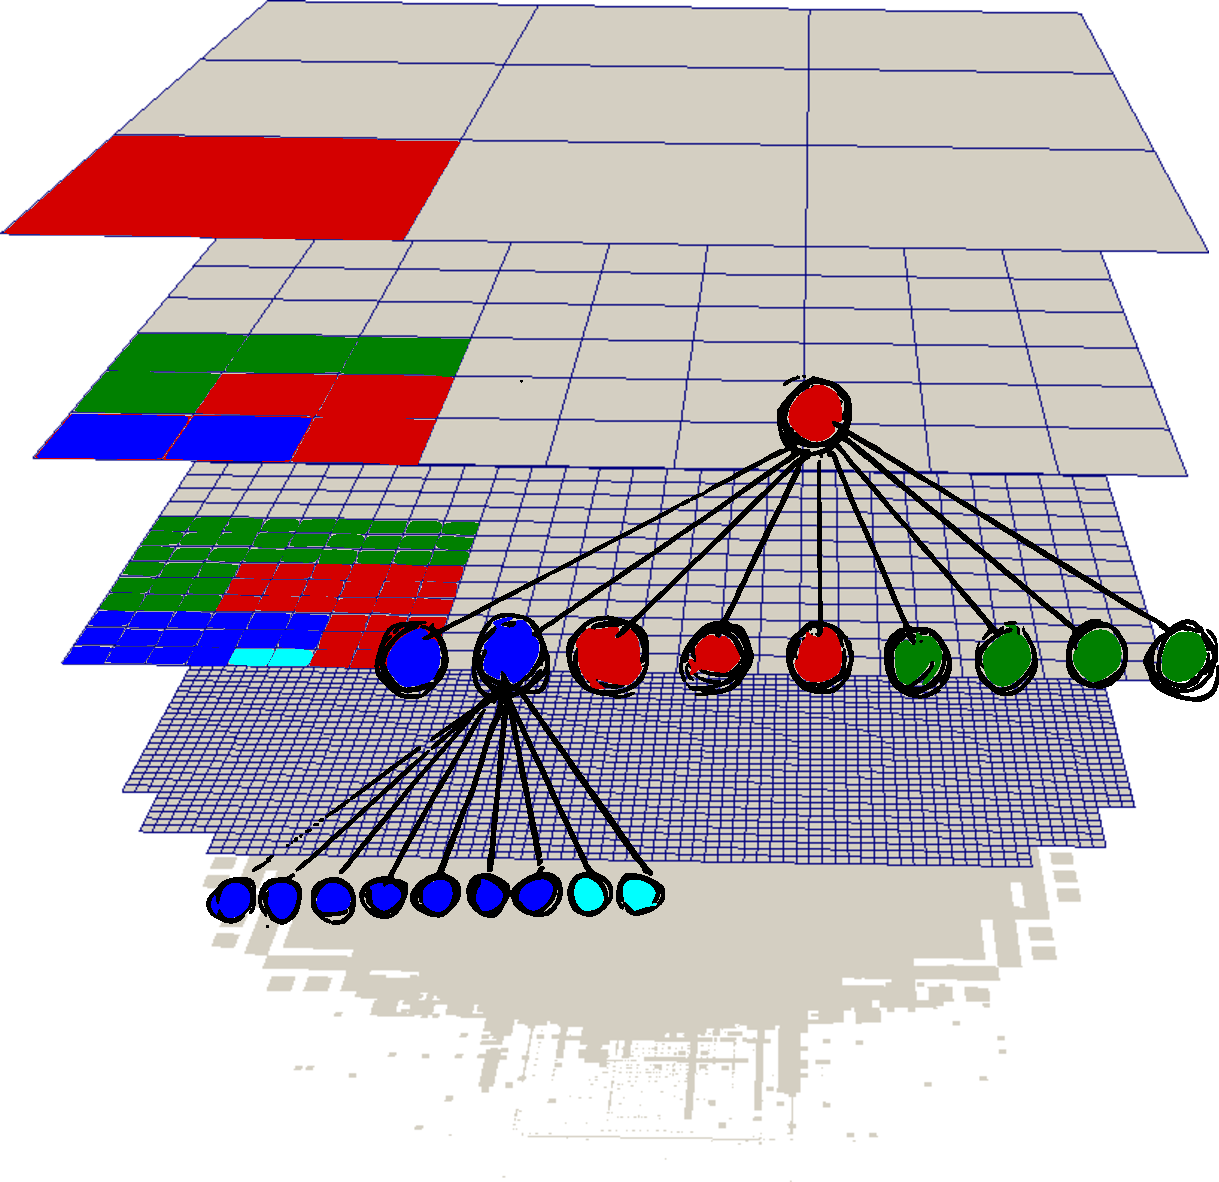
\includegraphics[width=0.5\textwidth]{52_mpi/spacetree-decomposition-top-down.pdf}
\end{center}

\noindent
The picture above details Peano's MPI concept:
The spacetree is top-down split up among the ranks. 
In the present fragment, red is the ``highest'' rank.
When it receives a \texttt{iterate} message from the global master, it also
receives a copy of the master's state as well as a copy of the coarsest cell
belonging to red and its adjacent vertices.
All these data is redundantly stored on the master.
The received state is automatically made the local state.
If you want to do something with the coarsest red cell or the four vertices
belonging to the coarsest level, you can realise 
\begin{code}
void mergeWithWorker(
  exahype::Cell&                               localCell, 
  const exahype::Cell&                         receivedMasterCell,
  const tarch::la::Vector<DIMENSIONS,double>&  cellCentre,
  const tarch::la::Vector<DIMENSIONS,double>&  cellSize,
  int                                          level
);

void mergeWithWorker(
  exahype::Vertex&                             localVertex,
  const exahype::Vertex&                       receivedMasterVertex,
  const tarch::la::Vector<DIMENSIONS,double>&  x,
  const tarch::la::Vector<DIMENSIONS,double>&  h,
  int                                          level
);
\end{code}

\noindent
in one of your mappings. 
Linear algebra codes transfer the residuals or correction values from vertices
through the individual levels.


With all data received, the red node starts to traverse its own tree. 
It recognises that is in turn is the master to two other ranks (green and blue)
and forwards its received state to these guys---as well as the corresponding
cells and vertices on the coarsest common level that the master and its workers
hold redundantly.

Afterwards, red continues to run through its local tree. 
When it starts to ascend through its local tree, it waits for its two workers
(green and dark blue) to terminate and receives from them a state as well as
copies of their coarsest cell plus the adjacent vertices.
This time, the state is not merged into anything automatically. 
However, you can realise the corresponding merge operations to restrict a global
residual value for example.


\subsection{Exchanging boundary data}

Peano realises a non-overlapping domain decomposition on each individual
resolution level.
This means that no cells are held redundantly between two neighbouring ranks on
the same level.
Only the coarsest cell of a rank is also held redundantly by its
master if we compare to \texttt{mergeWithWorker}, e.g.
Boundary data exchange thus exclusively affects vertices. 
It is important to note that all vertices on all levels that are adjacent to
cells of different ranks are exchanged per iteration.
You can switch off the boundary exchange explicitly, but this is subject of
discussion later on as it is a very specific optimisation that is of relevance
only for very few applications.


Mirroring the state behaviour, the code does not literally exchange all
attributes of the vertices.
It exchanges only those attributes of \texttt{Vertex} that are explicitly marked
with \texttt{parallelise} in the DaStGen definition file.  
Yet, exchange means solely that data is sent from one rank to the other and the
other way round---the term does not comprise how data from two vertices held by
two ranks are merged into each other.
Without any merge, copies of vertices along a domain's boundary are sent to all
other ranks per grid sweep, but nothing happens further, i.e.~the exchanged data
is dropped.
To change this, there is the plug-in point

\begin{code}
void prepareSendToNeighbour(
  exahype::Vertex&                             vertex,
  int                                          toRank,
  const tarch::la::Vector<DIMENSIONS,double>&  x,
  const tarch::la::Vector<DIMENSIONS,double>&  h,
  int                                          level
);
\end{code}

\noindent
Whenever a rank finds out that it has just used a vertex for the very last time
throughout a traversal---this happens right after \texttt{touchVertexLastTime}
has been called---and that this vertex is adjacent to multiple ranks and thus
stored on multiple ranks, it calls \texttt{prepareSendToNeighbour} for this
vertex per communication partner \texttt{toRank}.
This operation gives every mapping the opportunity to plug into the send
mechanism.

Peano exchanges its data similar to the Jacobi scheme in linear algebra: 
at the end of an iteration, it sends away copies of vertices. 
Prior to the subsequent traversal, it receives this data and allows the user to
merge it into the local data structures.
For the latter, there is another plug in point:
\begin{code}
void mergeWithNeighbour(
  exahype::Vertex&                              vertex,
  const exahype::Vertex&                        neighbour,
  int                                           fromRank,
  const tarch::la::Vector<DIMENSIONS,double>&   x,
  const tarch::la::Vector<DIMENSIONS,double>&   h,
  int                                           level
);
\end{code}

\noindent
This operation hands you over the local vertex copy as well as the received data
from every other adjacent rank.
While Peano ensures that all grid refinement data, e.g., is kept consistently,
it is your job to ensure that all application-specific data is kept consistent.

A simple matrix-free Jacobi iteration on the vertices thus reads as follows:
\begin{enumerate}
  \item When a vertex is loaded for the very first time throughout a traversal,
  we set its residual to $0$. This happens in \texttt{touchVertexFirstTime()}.
  \item In \texttt{enterCell}, the local residual of this vertex is accumulated.
  \item As soon as we receive \texttt{touchVertexLastTime()} of a particular
  vertex, we know that the code has run through all adjacent cells before. The
  residual hence is complete and we can update the vertex solution according to
  the Jacobi update scheme.
\end{enumerate}

\noindent
This workflow transfers as follows to a distributed memory environment:
\begin{enumerate}
  \item When a vertex is loaded for the very first time throughout a traversal,
  we set its residual to $0$. This happens in \texttt{touchVertexFirstTime()}.
  \item In \texttt{enterCell}, the local residual of this vertex is accumulated.
  \item As soon as we receive \texttt{touchVertexLastTime()} of a particular
  vertex, we know that the code has run through all adjacent cells before {\em
  if the vertex is  a local one}. We can check this with the operation
  \texttt{isAdjacentToRemoteRank()}. The residual hence is complete and we can update the
  vertex solution according to the Jacobi update scheme.
  \item Of a vertex is adjacent to any other rank, we may not update its value.
  We know that this vertex is sent away at the end of the iteration through 
  \texttt{prepareSendToNeighbour}. We do not change any data of the vertex
  herein.
  \item Prior to the next \texttt{touchVertexFirstTime()} on any other rank, we
  know that this rank will receive our local copy of the vertex in
  \texttt{mergeWithNeighbour}. We thus make \linebreak
  \texttt{mergeWithNeighbour} take any
  incoming vertex copy, take the residual from there and merge it into the local
  residual.
  \item If we run into \texttt{touchVertexFirstTime()} for a vertex with
  \texttt{isAdjacentToRemoteRank()}, we know that we didn't update its value yet
  because it had bee incomplete in the previous \texttt{touchVertexLastTime()}
  call. We however know that its residual is accumulated between domain
  boundaries now. We thus update and continue with the standard \linebreak
  \texttt{touchVertexFirstTime()}.
\end{enumerate}



\subsection{Exchanging boundary data on the heap}

Different to the vertex boundaries, heap data is not automatically exchanged by
Peano's MPI. 
There are different variants how to manage heaps. 
The simplest one is to instruct Peano via the communication specification that
you use a heap and want the code to exchange heap data along the domain
boundaries.
For this, your mappings have to define a communication specification
that sets the third flag to \texttt{true}.
By default, the generated specification uses \texttt{false}. 
Setting the flag instructs the Peano kernel that you want to use
heaps for boundary data exchange as well.
\begin{code}
peano::CommunicationSpecification  
myMapping::communicationSpecification() { 
  return peano::CommunicationSpecification( ...,...,true );
}
\end{code}

\noindent
The flag tells Peano that heaps are used for communication and that you want the
kernel to synchronise all communication channels. 
Notably, the kernel now ensures that all data is received before you start a new
traversal, and it releases data sent via nonblocking MPI automatically once a
traversal terminates.

\begin{remark}
If you fuse multiple mappings onto one adapter and one of the mappings specifies
\texttt{true} while all other mappings do not set this flag, then Peano will
administer the heap, i.e.~the single \texttt{true} dominates the behaviour.
However, you'll receive warnings that the various communication specifications
are inconsistent with each other. To remove those warnings, ensure that all
mappings either set the flag or not.
\end{remark}


Yet, no actual bundary data is sent and received yet. 
If you want to exchange data through a boundary vertex, you have to do so
explicitly in \texttt{prepareSendToNeighbour}.
Please note that Peano's heap has specialised operations for this:
\begin{code}
void myMapping::prepareSendToNeighbour(
  particles::pidt::Vertex&                      vertex,
  int                                           toRank,
  const tarch::la::Vector<DIMENSIONS,double>&   x,
  const tarch::la::Vector<DIMENSIONS,double>&   h,
  int                                           level
) {
  MyHeap::getInstance().sendData(
    index-of-heap-entry,
    toRank,
    x,
    level,
    peano::heap::MessageType::NeighbourCommunication
  );
}
\end{code}

\noindent
The counterpart has to be realised in \texttt{mergeWithNeighbour}.
Peano takes care that all data is exchanged in the right order as efficiently as
possible.

\begin{remark}
You are responsible to ensure that each heap send operation has a
corresponding receive on the other side for exactly the same vertex in the next
grid sweep.
As the data exchange is distributed between two iterations, you might decide to
implement the receive in a different mapping.
However, you have to ensure that each send is mapped by exactly one receive on
the vertex counterpart.
\end{remark}

\noindent
Instead of relying on the \texttt{true} flag in the specification, you can
decide to administer all the heaps yourself. 
If you do this, you have instruct the heap in \texttt{beginIteration} that you
start to exchange data (via the operation \texttt{startToSendBoundaryData}),
while you tell Peano in \texttt{endIteration} that this exchange has finished
through \texttt{finishedToSendBoundaryData}.


Most codes work fine with an automated heap data exchange administration. 
However, with a manual instruction, you are allowed to send out data in one
iteration and receive it a couple of iterations later.
The manual exchange operations of the heap class ensure that all data is
exchanged in the right order. 
You have to ensure that the number of sends and receives as well as the ordering
which vertex sends and receives match.
If you allow Peano to squeeze one or more traversals in-between a send and the
subsequent receive, you release pressure from MPI: 
Peano deploys all heap data exchange to non-blocking sends and receives.
It now has more time to transfer the actual data.
 


\subsection{Exchanging heap data vertically (in-sync)}

The previous paragraphs discussed the exchange of heap data between different
adjacent partitions. 
We call this horizontal data exchange (within a level).
If you want to exchange data between masters and workers or the other way round,
you can still rely on the heap's send and receive operations.
However, the data transfer semantics change.


Exchange between masters and workers is synchronous.
We do not send out data in one iteration and receive it in the subsequent
iteration, but we want to send out data when we descend into a worker tree node,
and this data has to be received just before this worker actually starts its
traversal.
To trigger this behaviour, you can still use the heap's send and receive, but
you have to pass 
\texttt{peano::heap::MessageType::MasterWorkerCommunication} as last argument.
This tells Peano that you want synchronous data exchange.


The heaps still work with non-blocking data transfers of MPI.
This helps to avoid blocking buffers and, thus, deadlocks. 
Therefore, we also have to tell the heap when you start a synchronous data
exchange and when you finish it.
For this, there are routines \texttt{startToSendSynchronousData} and
\texttt{finishedToSendSynchronousData} offered by every heap.


\begin{remark}
While Peano is built to use localised point-to-point messages only, you may want
to exchange data between any two ranks. The heaps allow you to do so---either
similar to a boundary data exchange where sent data is to be received in the
subsequent grid sweep or similar to a master-worker communication where sent
data is received right away.
\end{remark}


\begin{remark}
(Dynamic) Load balancing transfers data from one MPI rank to another one
synchronously: either from a master to a new worker when we split up a partition
or from a worker to a master if we merge two partitions into one subdomain. If
you have to transfer heap data here, you can apply the same pattern you've used
for master-worker data transfer. However, you should use the flag  
\texttt{peano::heap::MessageType::ForkOrJoinCommunication} rather than 
\texttt{peano::heap::MessageType::MasterWorkerCommunication} in your send and
receive calls.
Peano then uses different MPI tags and thus ensures that master-worker messages and fork-join
transfer data is not mixed up.
For the fork/join data, the heap requires no notification that data exchange
starts or stops; the kernel internally knows this already.
\end{remark}


\subsection{Running global steps on all ranks and manually broadcast
information from the global master}

Not all algorithms decompose exclusively into a sequence of grid sweeps. 
Software with explicit matrix assembly, e.g., maps the matrix assembly itself,
all plotting, postprocessing, time stepping and so forth onto grid traversals.
The global solve (via PETSc, e.g.) however is a plain function call per MPI
rank.
We may introduce an adapter/mapping for this, switch to this adapter on the
global master and trigger the adapter iterate on the global master.
The corresponding mapping for such a global step then however is almost trivial:
it does something in \texttt{beginIteration} or \texttt{endIteration} while the
actual grid traversal remains empty. 
Though such a translation of global steps into grid sweeps follows the pure
Peano philosophy, it is neither convenient to program nor is it efficient.
It is a waste of resources as the whole grid is piped through
the traversal once for the global step.


As alternative to the sketched variant, Peano's repository offers a
routine \texttt{runGlobalStep} while each worker implements a
\texttt{runGlobalStep}, too. 
To let all non-idle MPI ranks do one thing at a time, you implement the
following steps:

\begin{enumerate}
  \item Inside your global master's code, i.e.~somewhere within
  \texttt{runAsMaster}, you call \texttt{runGlobalStep} on your repository.
  \item You implement \texttt{runGlobalStep} in your runner. The repository call
  invokes this routine on all non-idle workers.
  \item If you want the global master to run through your runner's
  \texttt{runGlobalStep}, too, you have to call this one manually.
\end{enumerate}

The term non-idle in the paragraphs above refers to Peano's load balancing.
MPI's load balancing oracles can decide which and how many ranks at any time are
participating in the computation.
The load balancing may decide that some MPI ranks are not used at a certain
time.
They remain idle;
and they are then not affected by the global step.


\texttt{runGlobalStep}'s signature is empty.
We can start one routine simultaneously on all non-idle ranks, but we can not
natively hand over data.
However, you are always free to send data via MPI yourself. 
There are a few remarks on consider however and there are some support routines
that might be of value:

\begin{itemize}
  \item You can rely on plain MPI to exchange data. However, you can also model
  your messages with DaStGen which is convenient as DaStGen equips the modelled
  data structure with MPI send and receive commands.
  \item It is simple to receive data from and send data to the global master on
  the worker rankas, as the master's global rank number is available through the
  \texttt{Node}.
  \item The node pool offer a broadcast operation to send any message modelled
  with DaStGen out to all non-idle ranks.
  \item Alternatively (if you prefer to work with plain MPI, e.g.), it offers a
  query to ask for each rank whether it is idle or not.
  \item The node pool allows you to obtain an MPI tag. It is highly recommended
  to make your own global communication run through MPI tags of their own. This
  way, you ensure that your data sends and receives to not interfer with other
  MPI messages of Peano still pending in the network.
\end{itemize}

\noindent
Via the exchange of MPI messages within \texttt{runGlobalStep}, you can
implement different steps: you can basically send around an integer or enum
which triggers different behaviour on the ranks.
Below is an example of a manual global data distribution that relies on plain
MPI. 
As highlighted, modelling the messages with DaStGen yields shorter and more
elegant code:

\begin{code}
  const int myTag = tarch::parallel::Node::getInstance().reserveFreeTag(...);

  double myValue = 2; // you might want to use a DaStGen class instead of primitive types

  if (tarch::parallel::Node::getInstance().isGlobalMaster()) {
     double receivedValue;
     for (int rank=1; rank<tarch::parallel::Node::getInstance().getNumberOfNodes(); rank++) {
       if ( !tarch::parallel::NodePool::getInstance().isIdleNode(rank) ) {
         MPI_Recv( &receivedValue, 1, MPI_DOUBLE, rank, myTag,
           tarch::parallel::Node::getInstance().getCommunicator(),
           MPI_STATUS_IGNORE ); // would be a simple method invocation with DaStGen objects 
         myValue += receivedValue;
       }
     }
  }
  else {
    MPI_Send( &myValue, 1, MPI_DOUBLE, tarch::parallel::Node::getGlobalMasterRank(),
      myMessageTagUseForTheReduction, tarch::parallel::Node::getInstance().getCommunicator() );
  }

  tarch::parallel::Node::getInstance().releaseTag(myTag);
\end{code}


\subsection{Wrap-up, preparatory work and per-sweep pre- and postprocessing
on a worker}

In large codes, there's often a need to plug into the creation of a rank
(everytime it is used by the load balancing to handle a part of the grid) or to
run some pre- and postprocessing steps per grid traversal. 
To do so, you may add code to the pregenerated \texttt{RunnerParallelWorker.cpp}
file that even contains, if created by the development toolkit, some remarks
where to add source code.


\subsection{Further MPI remarks}

\begin{itemize}
  \item If you couple Peano with another component using MPI, and the two codes
  shall not interfer with collectives, you can change Peano's {\textbf
  communicator}.
  For this, have a look into \texttt{tarch::parallel::Node}. All Peano kernel
  routines ask the \texttt{Node} class which communicator to use. So change it
  there and you switch Peano to a different communicator.
  \item Peano uses various MPI {\textbf tags} to exchange data. Most Peano
  components grab a tag from a central data base and then work with this tag,
  i.e.~the tags are hidden from the user. If you want to exchange your own data
  with MPI commands and want to ensure not to interfer with any Peano messages,
  use the static operation \texttt{reserveFreeTag} from \linebreak
  \texttt{tarch::parallel::Node} in the system setup to reserve a tag for your
  own purposes that then exclusive to you.
  \item If you want to exchange data along the master-worker {\textbf topology} or
  with the {\textbf global rank}, it is best to ask the
  texttt{tarch::parallel::NodePool} for the right ranks. Usually, rank 0 is the
  global master. However, Peano can be reconfigured to change this
  behaviour---which is particularly useful if you couple the AMR framework with
  some other codes.
\end{itemize}



\subsection*{Further reading}

\begin{itemize}
  \item T. Weinzierl: 
  {\em The {P}eano software---parallel,
   automaton-based, dynamically adaptive grid traversals}.
  arXiv:1506.04496
  \item 
  T. Weinzierl and M. Mehl: {\em Peano---A Traversal and Storage Scheme for
Octree-Like Adaptive Cartesian Multiscale Grids}.
In R. Tuminaro, M. Benzi, X.-C. Cai, I. Duff, H. Elman, R. Freund, K. Jordan, T.
Kelley, D. Keyes, M. Kilmer, S. Leyffer, T. Manteuffel, S. McCormick, D.
Silvester, H. Walker, C. Woodward and I. Yavneh (ed.), SIAM Journal on
Scientific Computing, Volume 33{\textbf(5)} of Special Section: 2010 Copper Mountain
Conference, pp.~2732--2760, 2011.
  \item 
H.-J. Bungartz, W. Eckhardt, T. Weinzierl and C. Zenger: {\em A Precompiler to
Reduce the Memory Footprint of Multiscale PDE Solvers in C++}.
In P.M.A. Sloot (ed.), Future Generation Computer Systems, Volume 26{\textbf (1)},
pp.~175--182. Elsevier, 2010.
  \item 
T. Weinzierl: {\em A Framework for Parallel PDE Solvers on Multiscale Adaptive
Cartesian Grids}.
Dissertation, Institut f\"ur Informatik, Technische Universit\"at M\"unchen. Verlag Dr. Hut, M\"unchen, 2009.
    \item 
H.-J. Bungartz, M. Mehl, T. Weinzierl and W. Eckhardt: {\em DaStGen - A Data
Structure Generator for Parallel C++ HPC Software}.
In Bubak, van Albada, Sloot and Dongarra (ed.), ICCS 2008: Advancing Science
through Computation, Part III, Volume 5103 of Lecture Notes in Computer Science,
pp.~213--222. Springer-Verlag, Heidelberg, Berlin, June 2008.
\end{itemize}

% 
% % pdfor. pfor
% 
%   \chapter{Tuning}
%   \label{chapter:tuning}
% 
%   \section{Performance analysis}
\label{section:performance-analysis}

\chapterDescription
  {
    Less than 10 minutes unless you postprocess a big file.
  }
  {
    You may work with the plain output that Peano writes to the terminal. If you
    use log filters (cmp.~Chapter \ref{section:logging}), it is important that
    you know how to switch particular logging infos on. You also need a working
    Python installation.
  }

\noindent
Prior to any parallelisation or tuning discussion, I want to emphasise that it
usually makes sense first of all to have a how Peano is performing from a grid
point of view. For this, the framework comes along with a rather useful script.

\begin{itemize}
  \item Recompile your code with \texttt{-DPerformanceAnalysis}. For the
    performance analysis, it usually makes sense to compile with the highest
    optimisation level and to disable \texttt{-DDebug} and \texttt{-DAsserts}.
  \item Run your code and ensure that \texttt{info} outputs from the
    \texttt{peano::performanceanalysis} component are enabled.
  \item Pipe the output into a file:
    \begin{code}
> ./myExecutable myArguments > outputfile.txt
    \end{code} 
    We call this file \texttt{outputfile.txt} from hereon.
  \item Pass the output file to Peano's performance analysis script written in
  Python. Besides the script (name), you also have to tell the script how many 
    MPI ranks you have used and how many threads have been enabled. Skip
    the arguments if you haven't used MPI.
    \begin{code}
> python <mypath>/peano/performanceanalysis/performanceanalysis.py 
    \end{code} 
    Calling it without any options displays a usage message.
  \item Open the web browser of your choice and the generated files (typically
  your Peano output file with an additional \texttt{html} extension).
\end{itemize}

\begin{remark}
Besides the output written by Peano through the component
\texttt{peano::performanceanalysis}, you also have to use the
\texttt{CommandLineLogger} (the default), and you have to make this one write
out time stamps as well as trace information. If you use your own logger or a
modified log format, the Python script will fail.
All default logging options work as long as you don't use a log filter for
\texttt{performanceanalysis}.
\end{remark}

\begin{remark}
The present document suggests to pipe all output data from the terminal into a
file and to process this file. 
For many applications with low rank count this works fine.
The more ranks you have however the higher the probability that concurrent
writes to the terminal mess up your piped file.
In most cases, the performance analysis still succeeds. 
However, there are cases where the postprocessing fails.
In this case, it is better to use \texttt{setLogFormat} of the
\texttt{CommandLineLogger} to make the logger pipe output from different ranks
into different files.
There's an additional script in the \texttt{performanceanalysis} directory that
you can then use to fuse the various output files into one file before you start
the actual postprocessing.
\end{remark}



\noindent
If you browse through your directory, you will notice that all graphs are
written both as png and as pdf. 
You can thus integrate them directly into your \LaTeX\ reports.
Most generated graphs also are available in an increased resolution. 
These files have a \texttt{.large.} inserted into their extension.


\subsection*{Study phases of your code}

If you run the whole performance analysis over a longer Peano simultion, the
amount of data produced quickly becomes massive and hard to handle, and the generation of
these massive data even might pollute your results. 
In your code, you can always switch all performance analysis off. 
To do so, invoke
\begin{code}
  peano::performanceanalysis::Analysis::getInstance().enable(false);
\end{code}

\noindent
and call the same routine later on again with a \texttt{true} argument.

In a parallel environment, you have to switch the analysis on or off per rank,
i.e.~the analysis does not coordinate via MPI. 

\subsection*{Score-P/Scalasca}

We use Peano with Score-P\footnote{\url{http://www.vi-hps.org/projects/score-p}}
which is used by Scalasca\footnote{\url{http://http://www.scalasca.org/}}, e.g.
Score-P however tends to yield massive amounts of data. 
Peano can manually turn Score-P data aquisition on/off within the code. 
To enable this feature,
\begin{enumerate}
  \item retranslate your code with \texttt{-DUseScoreP},
  \item ensure you use the performance analysis as detailed above, and
  \item switch the performance analysis on and off suiting your demands as it is
  detailed in the previous paragraphs.
\end{enumerate}





%   \newpage
%   \section{General remarks}

\chapterDescription
  {
    Most remarks take less then 20 minutes.
  }
  {
    Working serial code.
  }


\subsection{Quick ('n not so dirty)}

\noindent
Peano by default keeps track of many grid statistics if you compile with
\texttt{-DTrackGridStatistics}.
For many codes, this is kind of an overkill: they do not require the whole
computer to keep track of all cells and vertices all the time, or, if they need
such data, they require more precise data; data also distinguishing more vertex
types than outer, inner, boundary, e.g.

If you don't need the state's getters on mesh width, number of vertices, and so
forth, try a recompile without \texttt{-DTrackGridStatistics}.


\subsection{Tailor your event specifications}

Before you start any optimisation, please run through all your mappings. 
Each mapping has a couple of specification routines that tells Peano whether
you have implemented the corresponding event, on which data is works (all
scales or only the leaves).
It is worth to make this as restrictive as possible to eliminate as many
operation evaluations as possible.
We assume that you have already specified the right shared memory concurrency
there.


%   \newpage
%   \section{Reducing the MPI grid setup and initial load balancing overhead}


\chapterDescription
  {
    Around 30 minutes.
  }
  {
    A working MPI code.
  }


In this section, we assume that you've a reasonable load balancing and that you
were able to postprocess your performance analysis outputs. We discuss issues
that arise over and over again for parallel applications.


\subsection{Massive grid on rank 0 with long redistribution phase
afterwards}

\begin{center}
  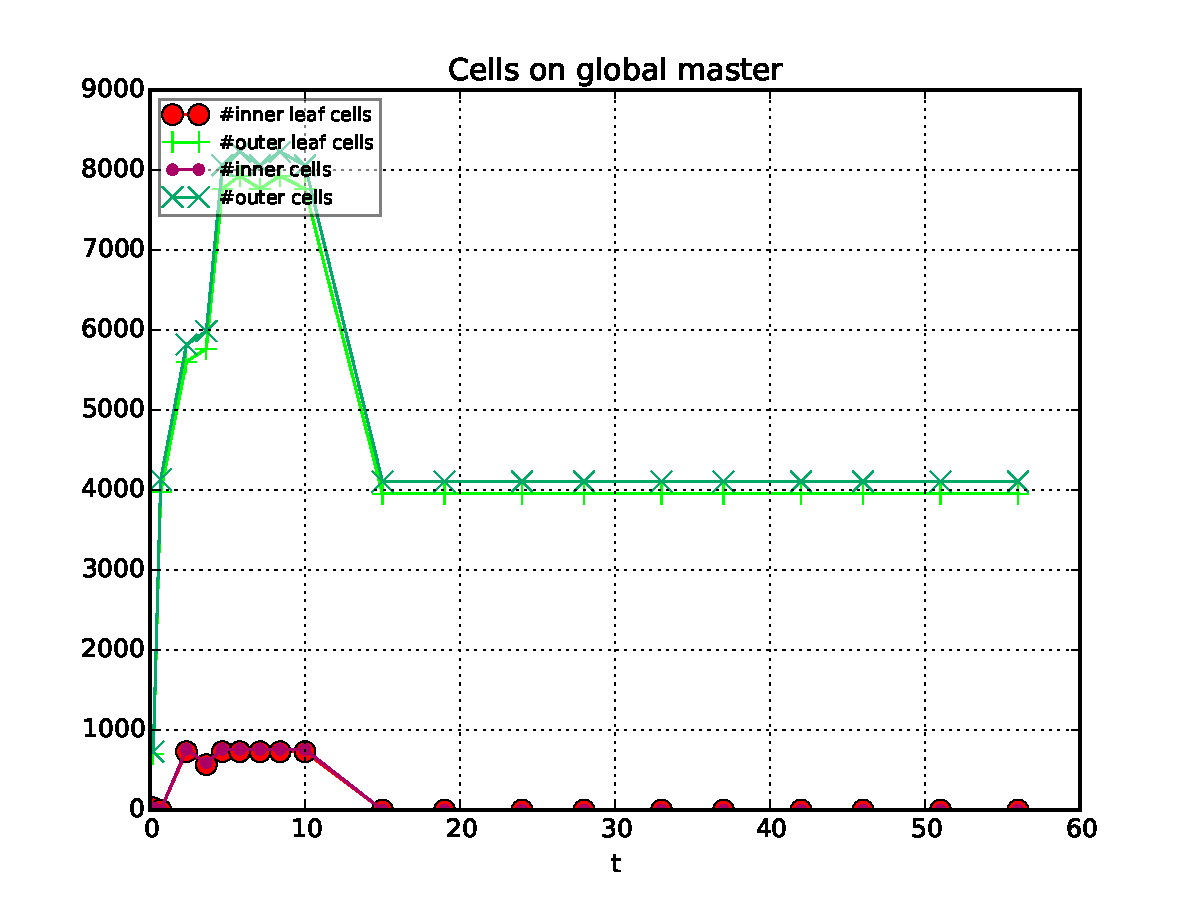
\includegraphics[width=0.5\textwidth]{61_mpi-setup/performance-analysis-output.pdf}
\end{center}


\begin{smell}
There are ranks (notably rank 0) that are assigned lots of cells and vertices
and then this number decreases though the grid should be more or less static.
\end{smell}

\noindent
We observe this behaviour either through a performance analysis (see plot above)
or by outputs from the state where the grid depth immediately goes up to the
maximum depth while the load balancing still splits up things. 
The iterations already are very expensive; obviously as the grid is already in
place but the ranks are not all employed.


The reason for this behaviour can be found in the semantics of
\texttt{createVertex} and \linebreak
\texttt{touchVertexFirstTime}.
Both operations try to refine the grid around the respective vertex immediately. 
Only if circumstances such as a parallel partitioning running through this
vertex---the refinement instruction then first has be distributed to all ranks
holding a copy of this vertex---do not allow Peano to realise the refinement
immediately, the refinement is postponed to the next iteration.
In many parallel codes, all the refinement calls pass through immediately on
rank 0 before it can spawn any rank.
This leads to the situation that the whole grid is in one sweep built up on the
global master and afterwards successively distributed among the ranks.


Such a behaviour is problematic: the global rank might run out of memory, lots
of data is transferred, and the sweeps over the whole grid on rank 0 are
typically pretty expensive. 
A distributed grid setup is advantageous.

\begin{solution}
Switch from an aggressive
refinement into an iterative grid refinement strategy to allow the ranks to
deploy work throughout the grid construction and thus build up the grid in parallel and avoid the transfer of whole grid
blocks due to rebalancing.
\end{solution}

\noindent
The simplest materialisation of this idea is to 
move your \texttt{refine()} calls from the creational or touch first
events into \texttt{touchVertexLastTime()}:
As a consequence, setting up a (rather regular) grid of depth $k$ requires at
least $k$ iterations.

\begin{remark}
 I typically extract the intial grid construction decision into a function of 
 its own. If \texttt{-DParallel} is used, I invoke grid constructions only 
 from \texttt{touchVertexLastTime}. Otherwise, I use it in the creational 
 routines for inner and boundary vertices. For this strategy, we have to ensure
 that touch last is not set to \texttt{Nop} in the specification attributes if
 we compile with MPI.
\end{remark}

In a second step, you might consider to extend your grid only every second
traversal.
Everytime you rebalance your grid, Peano disables dynamic load balancing
for a couple of iterations (three or four). Throughout these iterations, it
can recover all adjacency information if the grid itself changes as well.
Consequently, it does make sense to add a couple of adapter runs after each
grid modification that to not change the grid structure: When you know that
you have an adapter that changes the grid, apply afterwards an adapter that
does not change the grid for a couple of times. This way, you ensure that no
mpi rank runs out of memory. The grid generation does not overtake the rebalancing.
I often do not use an additional adapter but ensure that refines are only called
if the tree traversal direction is not inverted: 
Peano runs forth and back through the grid, so this effectively switches off
refinement every second iteration. 

The deluxe version is a code that refines only if the previous grid traversal
did not change the mesh, if no load balancing is going anymore and, for example,
\texttt{isTraversalInverted()} does not hold. This postpones any refinement
further.
However, such an approach is a bad idea if no idle nodes are available anymore. 
In this case, it is better not to veto the refinement anymore.
This situation is discussed in the following bad smell, where we propose a
sophisticated solution to both smells.



\subsection{Incremental, slow grid setup though detailed grid structure is
known/all nodes are already busy}


\begin{smell}
The grid is static, but, nevertheless, Peano needs lots of iterations to finally
build it up. Even worse, there are no idle nodes left and we know analytically
what the grid should look like.
The grid construction thus should rush through in one iteration.
\end{smell}


\noindent
Peano exchanges the vertices along a domain boundary after each traversal.
At the same time, it tries to refine a vertex with a refinement flag as soon as
possible: 
if a code sets a refine command upon creation of a vertex or when a vertex is
loaded for the very first time, it immediately refined.
If refine is called later throughout the traversal, Peano has to memorise the 
refinement request and wait for the subsequent traversal as all adjacent cells
have to anticipate an ongoing refinement but some have already been processed.
To ensure that the grid is always consistent, vertices at a domain boundary
never can be refined immediately. 
These guys are exchanged after each traversal and merged with their counterpart
on other ranks prior to the next usage. 
Refinement triggers thus never are available immediately on other ranks---these
vertices are replicated not held synchronous.

This behaviour implies that the grid can be built up at most by one level per
iteration along domain boundaries.
Therefore, we often see codes running many iterations until a regular grid is
built up completely.
Often, this is not necessary as all ranks would know without any data
exchange where to refine (a certain mesh size might be prescribed, e.g.).
For this case, Peano provides a function \texttt{enforceRefine} in the parallel
mode that tells the code not to bother about data consistency and to refine 
everywhere. 
Basically, the user tells the grid that he accepts responsibility to call 
\texttt{enforceRefine} on all replicants of a vertex.

We have to be very careful to use the enforced refinement.
We may use it if and only if there are no more idle nodes available and if all
previous forks and joins have successfully passed through. 
This is furthermore information that is available only on the global master. 

We thus propose to augment the \texttt{State.def} by a new flag:
\begin{code}
  #ifdef Parallel
  enum GridConstructionState {
    Default, Veto, Aggressive
  };
  
  parallelise persistent GridConstructionState  gridConstructionState; 
  #endif
\end{code}

\noindent
Per rank, we now create a copy of the global state that is propagated through
the tree (the state is used to determine the refinement strategy)
\begin{code}
  _localState = solverState;
\end{code}

\noindent
and we furthermore plug into the mapping's \texttt{endIteration} on modify this
global state on the global master. 
It has to be the global master as only the global master may ask the node pool
about idle nodes. 
Furthermore, it knows the (fork/join) state of all other ranks.
It is important to plug into \texttt{endIteration}, as this is the earliest
point where we have all information about the grid state at hands. 
The underlying status variables all are accumulated, i.e.~they might be already
cleared in the subsequent \texttt{beginIteration}:
\begin{code}
  if ( tarch::parallel::Node::getInstance().isGlobalMaster() ) {
    solverState.updateRegularInitialGridRefinementStrategy();
  }
\end{code}

\noindent
The state transitions then are
\begin{code}
void exahype::State::updateRegularInitialGridRefinementStrategy() {
  assertion( tarch::parallel::Node::getInstance().isGlobalMaster() );

  #ifdef Parallel
  if (
    tarch::parallel::Node::getInstance().getNumberOfNodes()==1
    ||
    _stateData.getGridConstructionState()==exahype::records::State::Aggressive
  ) {
    _stateData.setGridConstructionState( exahype::records::State::Aggressive );
  }
  else if (
    tarch::parallel::NodePool::getInstance().getNumberOfIdleNodes()==0
    &&
    isGridStationary()
  ) {
    _stateData.setGridConstructionState( exahype::records::State::Aggressive );
  }
  else if (
    isInvolvedInJoinOrFork()
    ||
    !isGridStationary()
  ) {
    _stateData.setGridConstructionState( exahype::records::State::Veto );
  }
  else {
    _stateData.setGridConstructionState( exahype::records::State::Default );
  }
  #endif
}

bool myproject::State::refineInitialGridInCreationalEvents() const {
  #ifdef Parallel
  return _stateData.getGridConstructionState() == myproject::records::State::Aggressive;
  #else
  return true;
  #endif
}

bool myproject::State::refineInitialGridInTouchVertexLastTime() const {
  #ifdef Parallel
  return _stateData.getGridConstructionState() != myproject::records::State::Veto;
  #else
  return false;
  #endif
}
\end{code}

\noindent
and we invoke our refinement from the creational vertex events as well as
\texttt{touchVertexLastTime} if the corresponding state predicates hold.
Finally, we make the refinement fall back to an enforced refinement if the state
permits us to do so:
\begin{code}
void myproject::mappings::RegularMesh::refineVertexIfNecessary(
  exahype::Vertex&                              fineGridVertex,
  const tarch::la::Vector<DIMENSIONS, double>&  fineGridH,
  bool                                          isCalledByCreationalEvent
) const {
  if (
    fineGridVertex.getRefinementControl() == Vertex::Records::Unrefined
    &&
    I want to refine and know this a priori
  ) {
    #ifdef Parallel
    if (isCalledByCreationalEvent) {
      fineGridVertex.enforceRefine();
    }
    else {
      fineGridVertex.refine();
    }
    #else
    fineGridVertex.refine();
    #endif
  }
}
\end{code}

% \begin{remark}
% If you decide to activate your grid refinement only every second iteration
% (\texttt{isTraversalInverted}), then it makes sense to do always two iterations
% in the loop body that runs the grid construction steps until
% \texttt{isGridBalanced} holds. This way, you never miss a refinement. 
% \end{remark}

\noindent
Creating a good runner that does not stop a grid setup too early, i.e.~before
the grid is built up completely and all load balancing has terminated, often
looks similar to
\begin{code}
int gridSetupIterations      = 0;
int gridSetupIterationsToRun = 3;
while (gridSetupIterationsToRun>0) {
  repository.iterate();
  gridSetupIterations++;
   
  if ( UseStationaryCriterion && repository.getState().isGridStationary() ) {
    gridSetupIterationsToRun--;
  }
  else if ( !repository.getState().isGridBalanced() && 
    tarch::parallel::NodePool::getInstance().getNumberOfIdleNodes()>0 ) {
    gridSetupIterationsToRun=3;  // we need at least 3 sweeps to recover from ongoing lb 
  }
  else if ( !repository.getState().isGridBalanced()  ) {
    gridSetupIterationsToRun=1;  // one additional step to get adjacency right
  }
  else {
    gridSetupIterationsToRun--;
  }
}
\end{code}


\begin{remark}
Often the pattern above still allows for a too aggressive grid creation if the
load balancing is very conservative and careful, i.e.~does only remove small
fragments of the domain at a time. If this is the case, I found it advantageous
to make the state of the global master memorise the number of idle ranks after
each decision. If it recognises that some load balancing just has happened, it
might decide to postpone further grid refinements.
  \begin{code}
void exahype::State::updateRegularInitialGridRefinementStrategy() {
  [...]
  else if ( 
      isInvolvedInJoinOrFork()
    ||
    !isTraversalInverted()
    ||
    !isGridStationary()
  ) {
    _stateData.setGridConstructionState( exahype::records::State::Veto );
  }
  else if (
    _idleRanksAtLastLookup != tarch::parallel::NodePool::getInstance().
      getNumberOfIdleNodes()
  ) {
    _stateData.setGridConstructionState( exahype::records::State::Veto );
    _idleRanksAtLastLookup = tarch::parallel::NodePool::getInstance().
      getNumberOfIdleNodes();
  }
  else {
    _stateData.setGridConstructionState( exahype::records::State::Default );
  }
  [...]
}

  \end{code}
\end{remark}

\subsection{The load balancing kicks in immediately while I build up my grid but it
yields non-reasonable partitions}


\begin{smell}
The code runs over the grid a couple of times and starts to distribute the
domain level-by-level as we rely on an incremental build-up. This is however not
clever as it turns out later throughout the grid construction that some regions
are heavily refined while others remain coarse.
\end{smell}


\noindent
If this is the case, it might be reasonable to build up the grid up to a certain
level where grid characteristics become visible, and to switch off the load
balancing while you do so.
Afterwards, load balancing can be enabled and should yield better results. 
Peano allows you to switch off the load balancing, but you have to do this on
each individual rank. 

\begin{code}
peano::parallel::loadbalancing::Oracle::getInstance().activateLoadBalancing(false);
\end{code}


You might want to use
\begin{code}
void myproject::runners::Runner::runGlobalStep() {
  // assertion( !peano::parallel::loadbalancing::Oracle::getInstance().
  // isLoadBalancingActivated() );

  peano::parallel::loadbalancing::Oracle::getInstance().activateLoadBalancing(false);
}
\end{code}

\noindent
to switch off load balancing globally.



\subsection{The load balancing seems not to use all ranks}

\noindent
Peano uses a subscriber pattern to manage all the MPI ranks, while rank 0 is
resopnsible for the actual load/rank assignments.
At startup, rank 0 knows nothing about all the other MPI ranks available.
They have to register at rank 0 (the node pool).
Ranks that want to shared work, ask at the node pool for free ranks and then get
assigned no co-workers.
It thus may happen that a rank asks at the node pool for idle MPI ranks and is
told that no rank is registers though the registration message was just pending
in the queue, i.e.~there would have been further MPI ranks available.
This happens rarely (you then might receive a fork failed notice; depending on
your load balancing), but there is another indicator.

\begin{smell}
  At startup, I receive a lot of messages alike \texttt{node pool does not
  contain entry for rank 3. Message from rank 3 might have overtaken
  registration message. Waiting for registration} if I compile with
  \texttt{-DAsserts}.
\end{smell}

\noindent
A solution to this problem is simple though it (very slightly) increases the
code's startup time.
Please note that it will not make this particular message go away:  
It usually shows up if a rank (here it is rank 3) requests work though its
registration message is still in the queue and hasn't been processed yet.

What you can do is invoke 
\begin{code}
  tarch::parallel::NodePool::getInstance().restart();
  tarch::parallel::NodePool::getInstance().waitForAllNodesToBecomeIdle();
\end{code}
\noindent
just after the restart.
The wait command degenerates to nop if you call it on a rank that is not the
global master, so it is save to call it on every rank.

%   \newpage
%   \section{MPI quick tuning}


\chapterDescription
  {
    Around 15 minutes.
  }
  {
    A working MPI code.
  }


This section collects a couple of really primitive measurements to make your
code faster.

\subsection{Filter out log statements}

It is probably to simple to mention, but all our teams from time to time forget
this. 
One of the major things slowing down codes is writing to the terminal. 
So adding a few additional log filters can significantly speed up your code.



\subsection{Switch off load balancing}

Most of Peano's load balancing algorithms (at least the ones coming along with
the standard package) rely on a central node pool.
If a rank decides that it would be advantageous to split up its domain, it sends
a request to the first rank whether there are any idle nodes available.
If your code already uses all ranks, this is a time consuming process that
suffers from latency.
If you know a prior that the load balancing is static and no further splits of
subdomains are possible, it does make sense to switch the load balancing off.
There is a routine \texttt{activateLoadBalancing} operation on the load
balancing oracle to do so.

This operation has to be called on each individual rank, i.e.~you can switch 
the load balancing on and off on a rank-per-rank basis. There are basically two
variants/patterns to disable the load balancing:
\begin{enumerate}
  \item You may introduce a new mapping that does nothing besides switching the
  load balancing off (typically in \texttt{beginIteration}). You then merge this
  mapping into your other adapters.
  \item You add a new bool to your state. In the global runner you set this
  boolean flag once you want to switch the load balancing off. The state then is
  successively propagated to the workers. In \texttt{beginIteration}, you
  analyse this bool (in any mapping) and you switch off the load balancing if
  the flag is set.
\end{enumerate}

Peano also offers the opportunity to invoke a
global step on all ranks prior to an \texttt{iterate} call.
This feature can be used to switch off the load balancing, too:

\begin{code}
void picard::runners::Runner::runGlobalStep() {
  peano::parallel::loadbalancing::Oracle::getInstance().activateLoadBalancing(false);
}


int picard::runners::Runner::runAsMaster(...) {
  ...
  
  repository.runGlobalStep(); // on all other ranks
  runGlobalStep();            // and locally, too
}
\end{code}

\noindent
As clarified in the documentation of the operations (see the autogenerated
header files of your repository, e.g.), you have to be careful if you follow
this variant:
You are never allowed to run a global step if any rank is involved in a join or
fork. 


%   \newpage
%   \section{Reduce MPI Synchronisation}


\chapterDescription
  {
    Around 60 minutes.
  }
  {
    A working MPI code.
  }


Peano has very strong constraints on the master-worker and worker-master
communication as the data exchange between these two is synchronous. It imposes
a partial order. If that slows down your application (you see this from the
mpianalysis reports), you can kind of weaken the communication constraints. 
Often, some data is not required immediately, not required globally all the
time, or doesn't have to be 100\% correct at all algorithmic stages. This
chapter discusses some things that you can do then.
So we assume that you have proper load balancing.


\begin{smell}
We face a very strong synchronisation.
This materialises in very regular execution patterns
where each rank waits for rank 0 to start up a new traversal.
It can also be reported by Peano's performance analysis.
\end{smell}

\begin{center}
  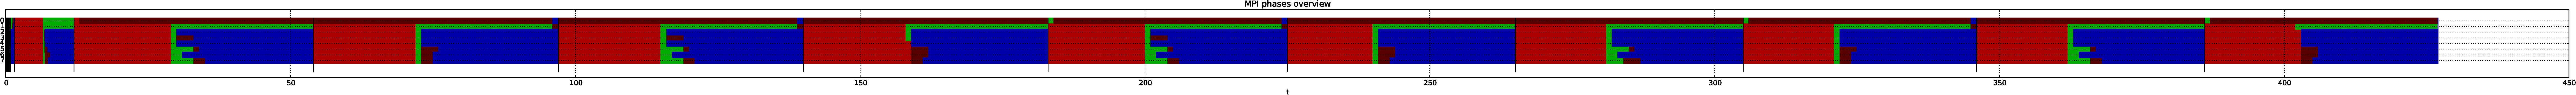
\includegraphics[width=0.9\textwidth]{63_mpi-synchronisation/mpi-phases-before.pdf}
\end{center}

\noindent
It also becomes obvious if you study how often a master has to work for its 
workers. 
In the picture below, only rank 0 synchronises the other ranks.
In this case, you have to weaken the global synchronisation.
If multiple of these edges pop up, it is time to weaken all the worker-master
synchronisations---unless you can identify that you have a load balancing issue.


\begin{center}
  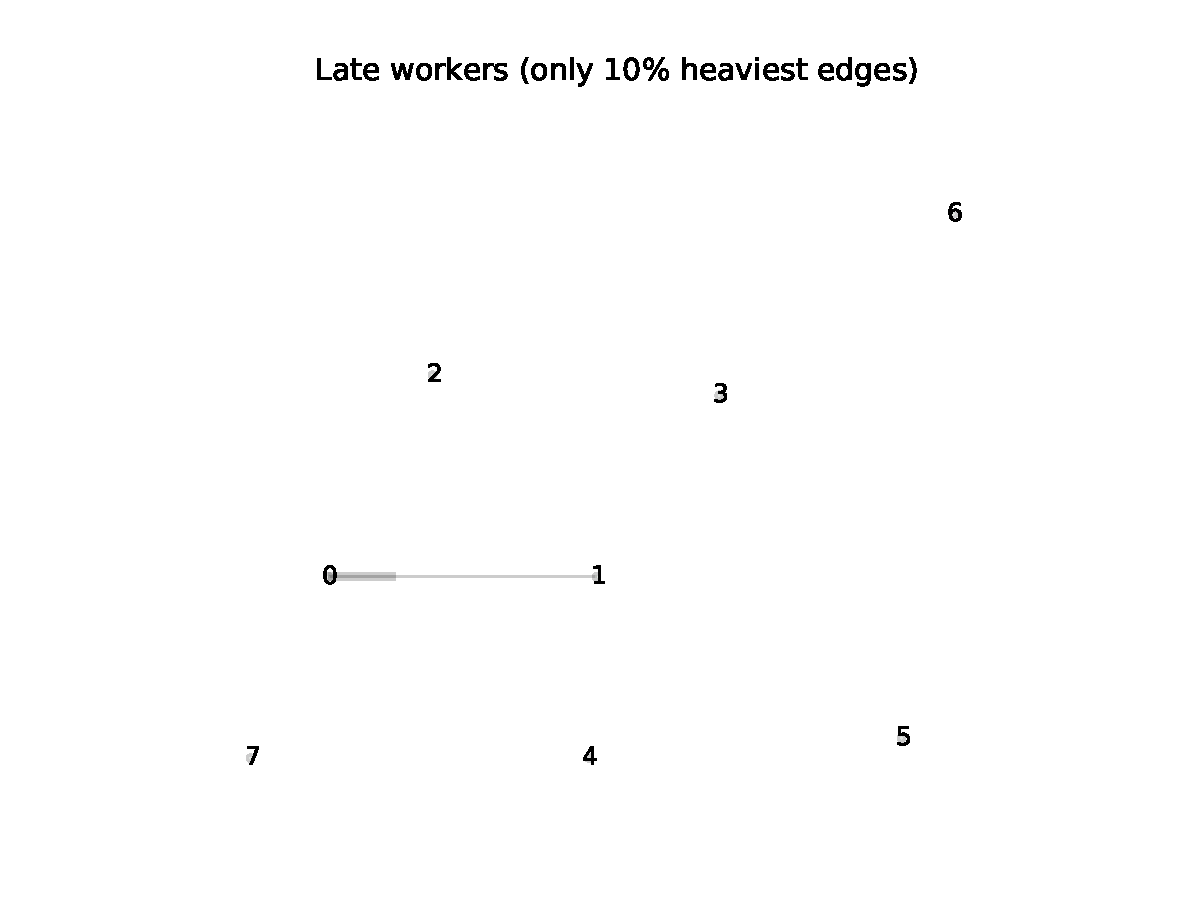
\includegraphics[width=0.5\textwidth]{63_mpi-synchronisation/master-worker-before.pdf}
\end{center}



\subsection{Postpone and tailor master-worker and worker-master data exchange}

In this section, we study the communication specification of the mappings. 
By default, they are set to the most general case:
Peano send away data from a local node if and only if it has traversed the whole local tree. 
In return, it requires all input data before it starts to traverse anything.

If you manage to send out data earlier, a rank's master can continue its local
traversal earlier.
If you manage to receive important data from the master, i.e.~from coarser
mesh levels, later, your rank can start its traversal right away when it is
informed which adapter is ran next.
This allows you to overlap computations more aggressively. 


\paragraph{Multiscale vertices and cells}

If a cell in the spacetree is deployed to another rank (grey cell in the sketch
below), the master continues to hold a replica of the deployed cell.
At the begin of a traversal, it sends the replica together with its parent cell
to the worker (blue instance) that is responsible for the actual data.
When the worker has finished its traversal, it sends the blue cell plus its
parent back to the master.
The same holds for the vertices adjacent to the cells.

\begin{center}
  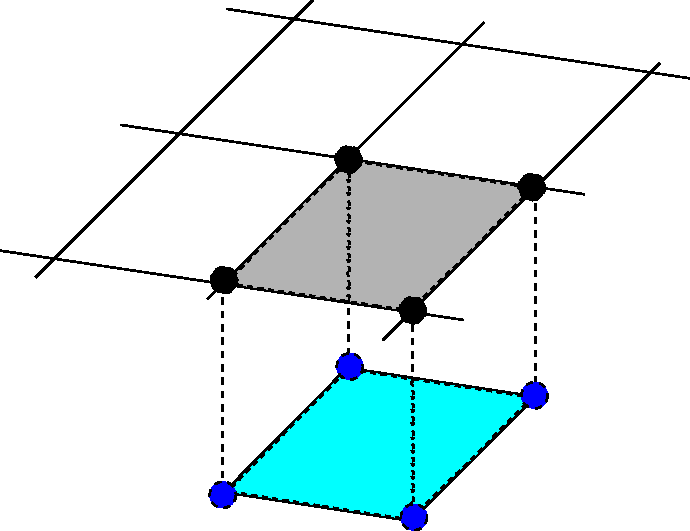
\includegraphics[width=0.35\textwidth]{63_mpi-synchronisation/master-worker.pdf}
\end{center}

\noindent
Such a workflow allows you to realise multiscale algorithms where information is
transferred through the cells or vertices from the master ot the worker and
back.
In return, the data exchange is rather critical as it runs synchronous.
The master is not allowed to fire up the worker to do its traversal before it
hasn't loaded all the vertices.
A similar reasoning holds the other way round.
Please note that the solver's state is exchanged along the very same lines,
i.e.~when we start up a worker and when the worker traversal terminates.


We notion that many codes do not require such a tight multiscale vertex
synchronisation.
If no multiscale data is exchanged at all, we do not need any of these
synchronous data sends and receives.
If we transfer data only through cells, we do not need the vertex copies before
we start the fine grid traversal.
We can wait until we do the very first \texttt{enterCell} on the worker.
Only if we need the copies of the vertices before the first
\texttt{touchVertexFirstTime}, we have to synchronise tightly.


\begin{remark}
In Peano, a cell that is deployed to a worker has exclusively refined adjacent
vertices. 
You can assume that a deployed cell (the greyish in the sketch) thus always is
refined.
\end{remark}


If you want tailor the data exchange, you have to open all the mappings you use
in your adapter.
There are two enumeration values that allow you specify exactly which data you
need at which time throughout a worker traversal.


\begin{remark}
Some codes may not skip multiscale data transfer all the time. See discussion in
the sections below on details.
\end{remark}


\subsection{Weaken synchronisation with global master}

\begin{center}
  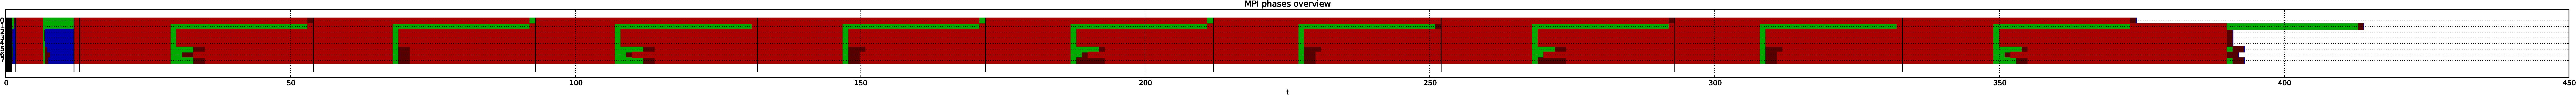
\includegraphics[width=0.9\textwidth]{63_mpi-synchronisation/mpi-phases-after.pdf}
\end{center}


\begin{smell}
The performance analysis reports on strong synchronisation and the traces show
that each new iteration on each rank coincides exactly with the start of a
global new step (vertical bars in plot).
\end{smell}


The global master (rank 0) is kind of a pulse generator for the whole code. 
Whenever the \texttt{runAsMaster} operation triggers \texttt{iterate}, it tells
each rank that handles a partition which adapter to use and to start its
traversal or wait for its master to trigger the traversal, respectively.
This is a very strong synchronisation.
Notably, no rank can continue to work with the next iteration unless rank 0 runs
into the next \texttt{iterate} as well.
There are basically two ways to improve this situation:

\begin{enumerate}
  \item Perform more than one time step with the same adapter and settings in a
  row. For this, use the integer argument of \texttt{iterate()}. Note that
  running multiple time steps switches off load balancing for this phase of the program.
  Obviously, this version works if and only if you run the same adapter several 
  times.
  \item You may alternatively find out that you don't need the rank 0 (that
  doesn't hold any data anyway) to wait for all the other ranks in each
  iteration. Often, you run for example a sequence of adapters and you require
  global data (such as global residual) only after the last run. 
  This second option (which is typically not a quick 'n dirty one) is discussed
  in the next subsection. 
\end{enumerate}



\subsection{Skip worker-master data transfer locally/sporadically}

We next discuss the decond variant.
Before we do so, we summarise typical smells that pop up once you have made 
your code run a fixed number of iterations:

\begin{smell}
You run multiple iterations with one \texttt{iterate} command but nevertheless
 \begin{itemize}
  \item the performance analysis identifies strong synchronisation or
  \item shows that some ranks permanently are late with their boundary data
  while the MPI trace shows that the traversals are kind of in sync.
 \end{itemize}
\end{smell}

\begin{center}
  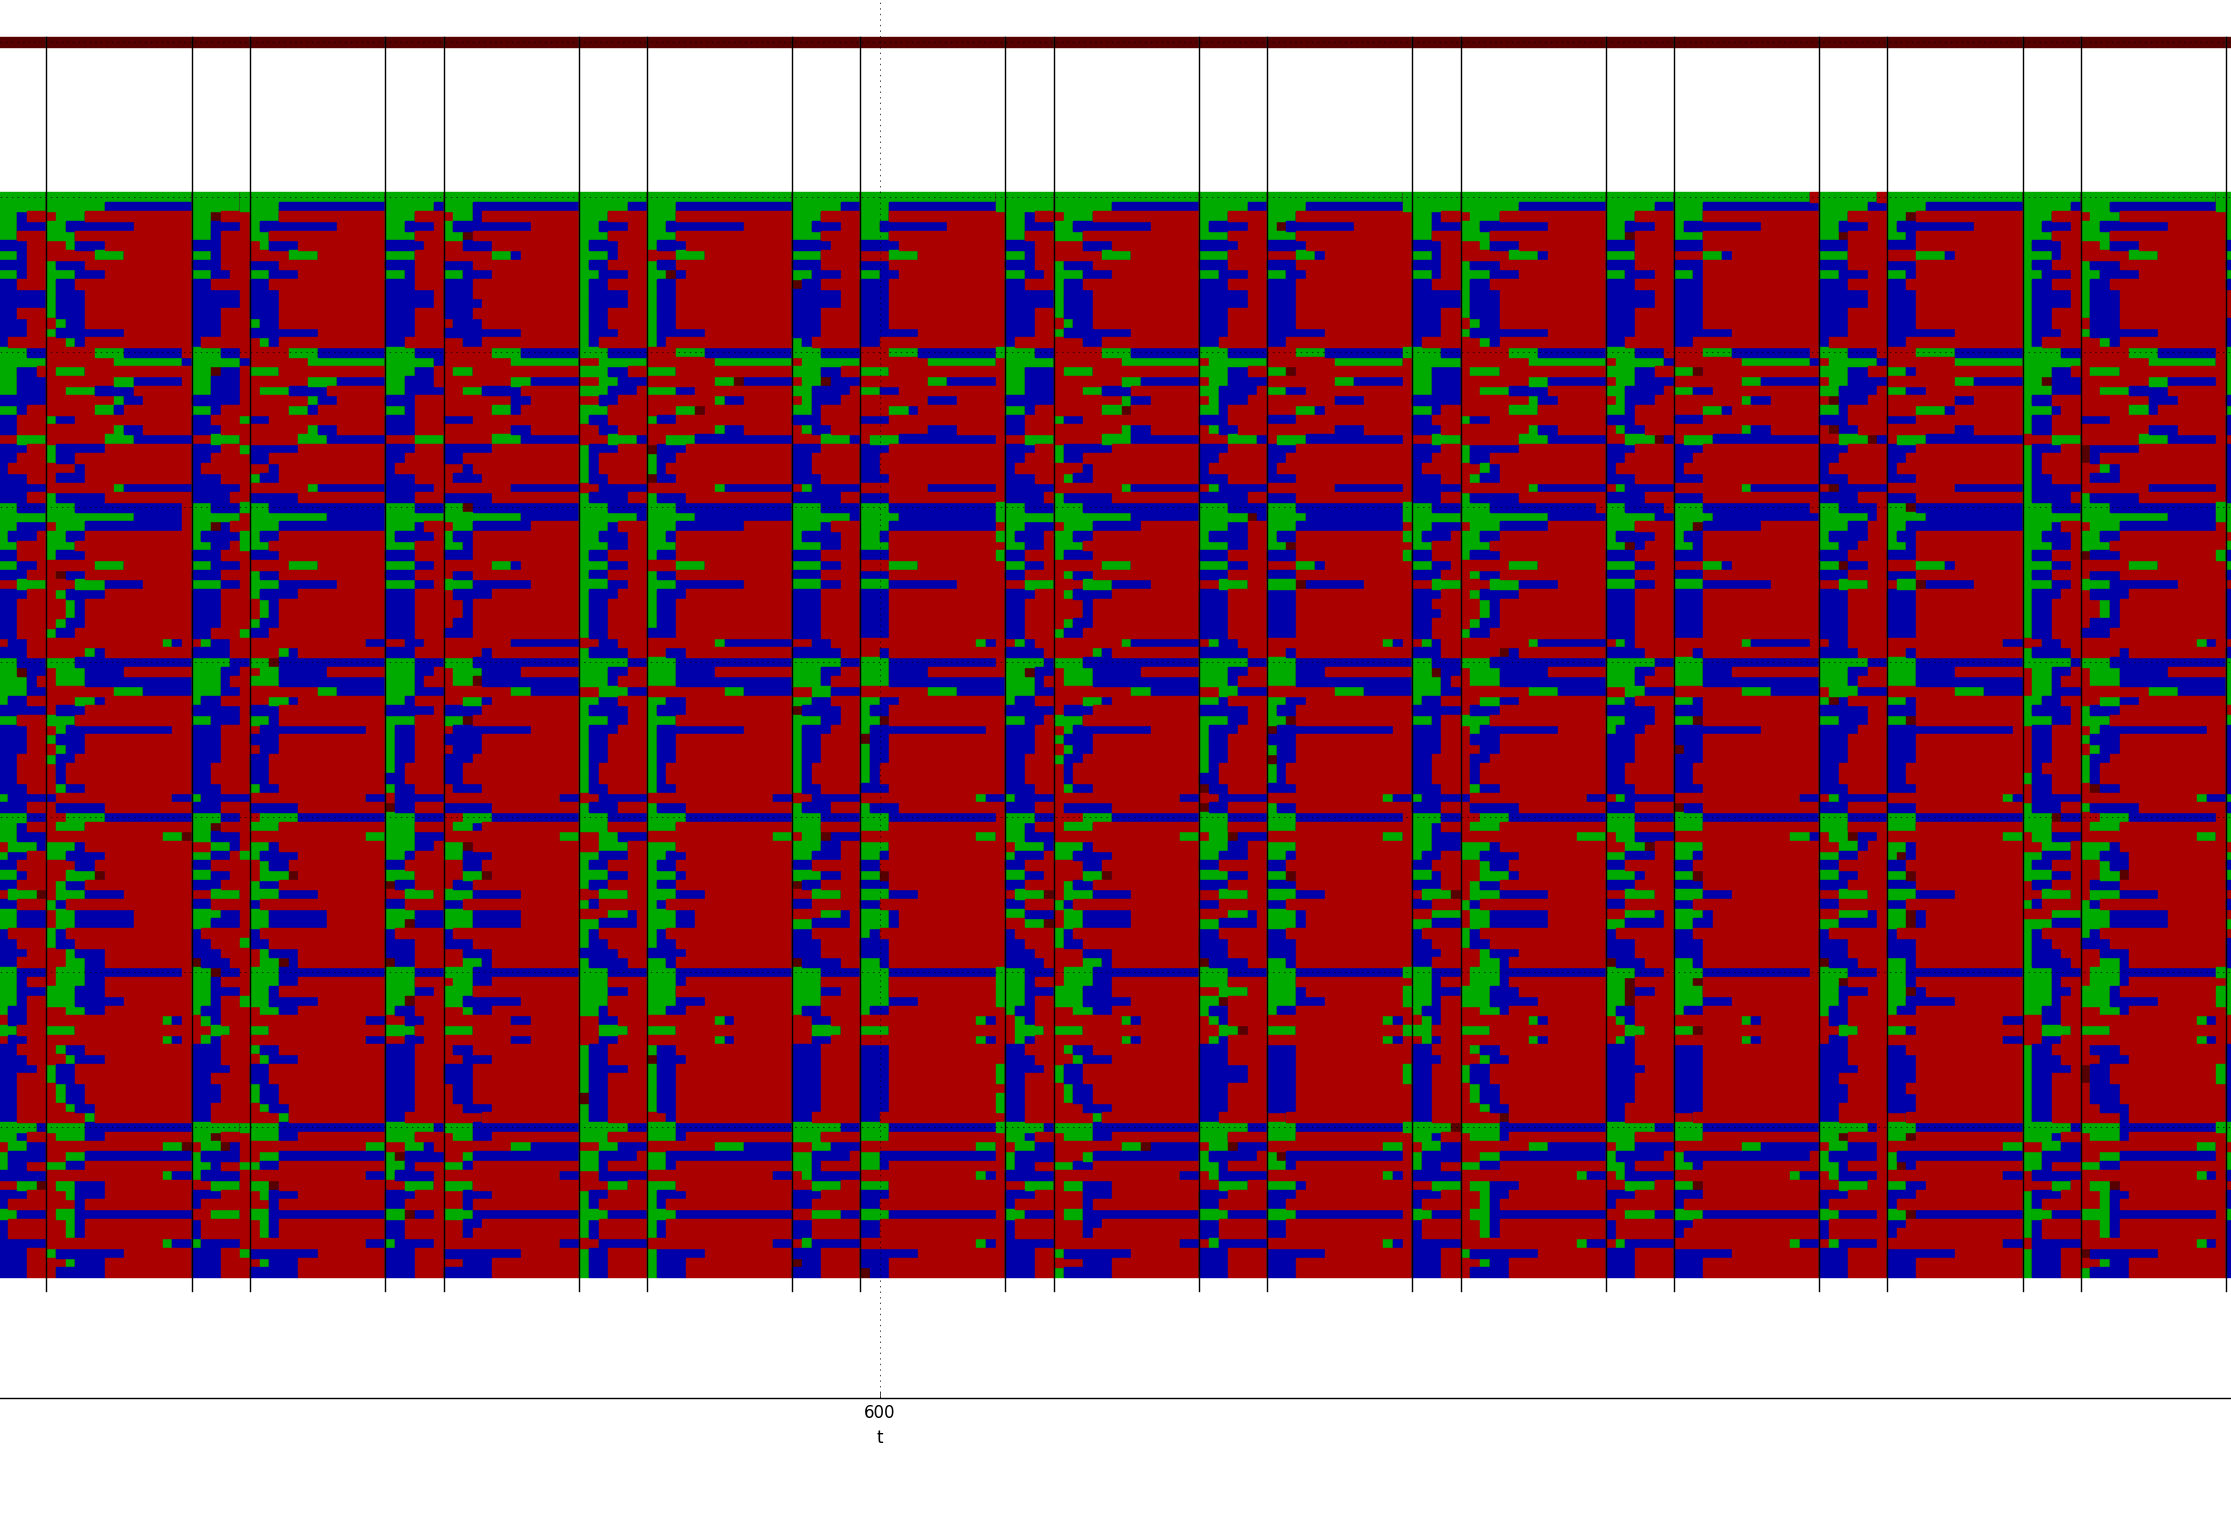
\includegraphics[width=0.7\textwidth]{63_mpi-synchronisation/no-skip-of-reduction.png}
\end{center}

\noindent
We see in the example above that the execution phases are in sync while the
report finds no later worker-master relation. 
Furthermore, we see an oscillating pattern: every second iteration lasts
significantly longer which materialises in zig zag timings for individual steps,
too.

Our goal in this step is to break up this synchronisation further which,
depending on your smell
\begin{itemize}
  \item eliminates late workers or
  \item allows more ranks to aggressively finish their boundary data exchange
  and thus free the interconnects from traffic.
\end{itemize}



If you want to realise the second variant, you have to
ensure that all mappings you use (also the predefined ones) return false in
\texttt{prepareSendToWorker(...)}.
  
\begin{remark}
  If you want to validate that reductions have been skipped, switch on the log
  info of 
  \texttt{peano::grid::nodes::Node::updateCellsParallel}
  \texttt{StateBeforeStoreForRootOfDeployedSubtree}.
\end{remark}


\noindent
Please be aware that reduction are skipped by the kernel if and only if all
mappings allow the kernel to switch off the reduction.
Furthermore, load balancing has to be disabled.
If you want to load balance, master and worker ranks have to communicate with
each other and may not skip any data/status exchange.

We also observe that the reduction skips often only change the communication
profile but do not speed up the computation. 
Often it is only a preparatory step to switch off boundary data exchange
afterwards.
Once this is done, you should get a profile as below. 
It is more or less completely asynchronous, and all data exchange (blue) is
hidden in the background, i.e.~not visible anymore:




Peano relies on a modified depth-first (dfs) traversal. The parallel variant also is a dfs, but whenever the dfs traversal encounters a remote node, it makes another mpi rank traverse the corresponding spacetree, while it continues itself with the local subtree. Before is ascends again, it checks whether the remote subtree traversals have terminates as well. As a result, it is important to split up the tree on an as coarse level as possible to obtain a high concurrency Level. Let's study a toy problem in 1d:


getCoarsestGridLevelOfAllSolvers()

%   \newpage
%   \section{Advanced MPI and boundary exchange optimisations}


\chapterDescription
  {
    The techniques discussed here are rather technical and/or non-trivial to
    implement, so realising them can be time-consuming.
  }
  {
    A working MPI code that scales to some degree.
  }



\subsection{Temporarilty switch off vertex data exchange}
\label{section:64_advanced-mpi:switch-off-vertex-data-exchange}

\begin{smell}
  The performance analysis identifies that some ranks slow down the computation
  as they send out their boundary data late, i.e.~others have to wait. When we
  study the distribution of the runtime of the involved ranks, we see that a
  significand rato of the per-traversal runtime is spent on boundary data
  exchange.
\end{smell}


\begin{center}
  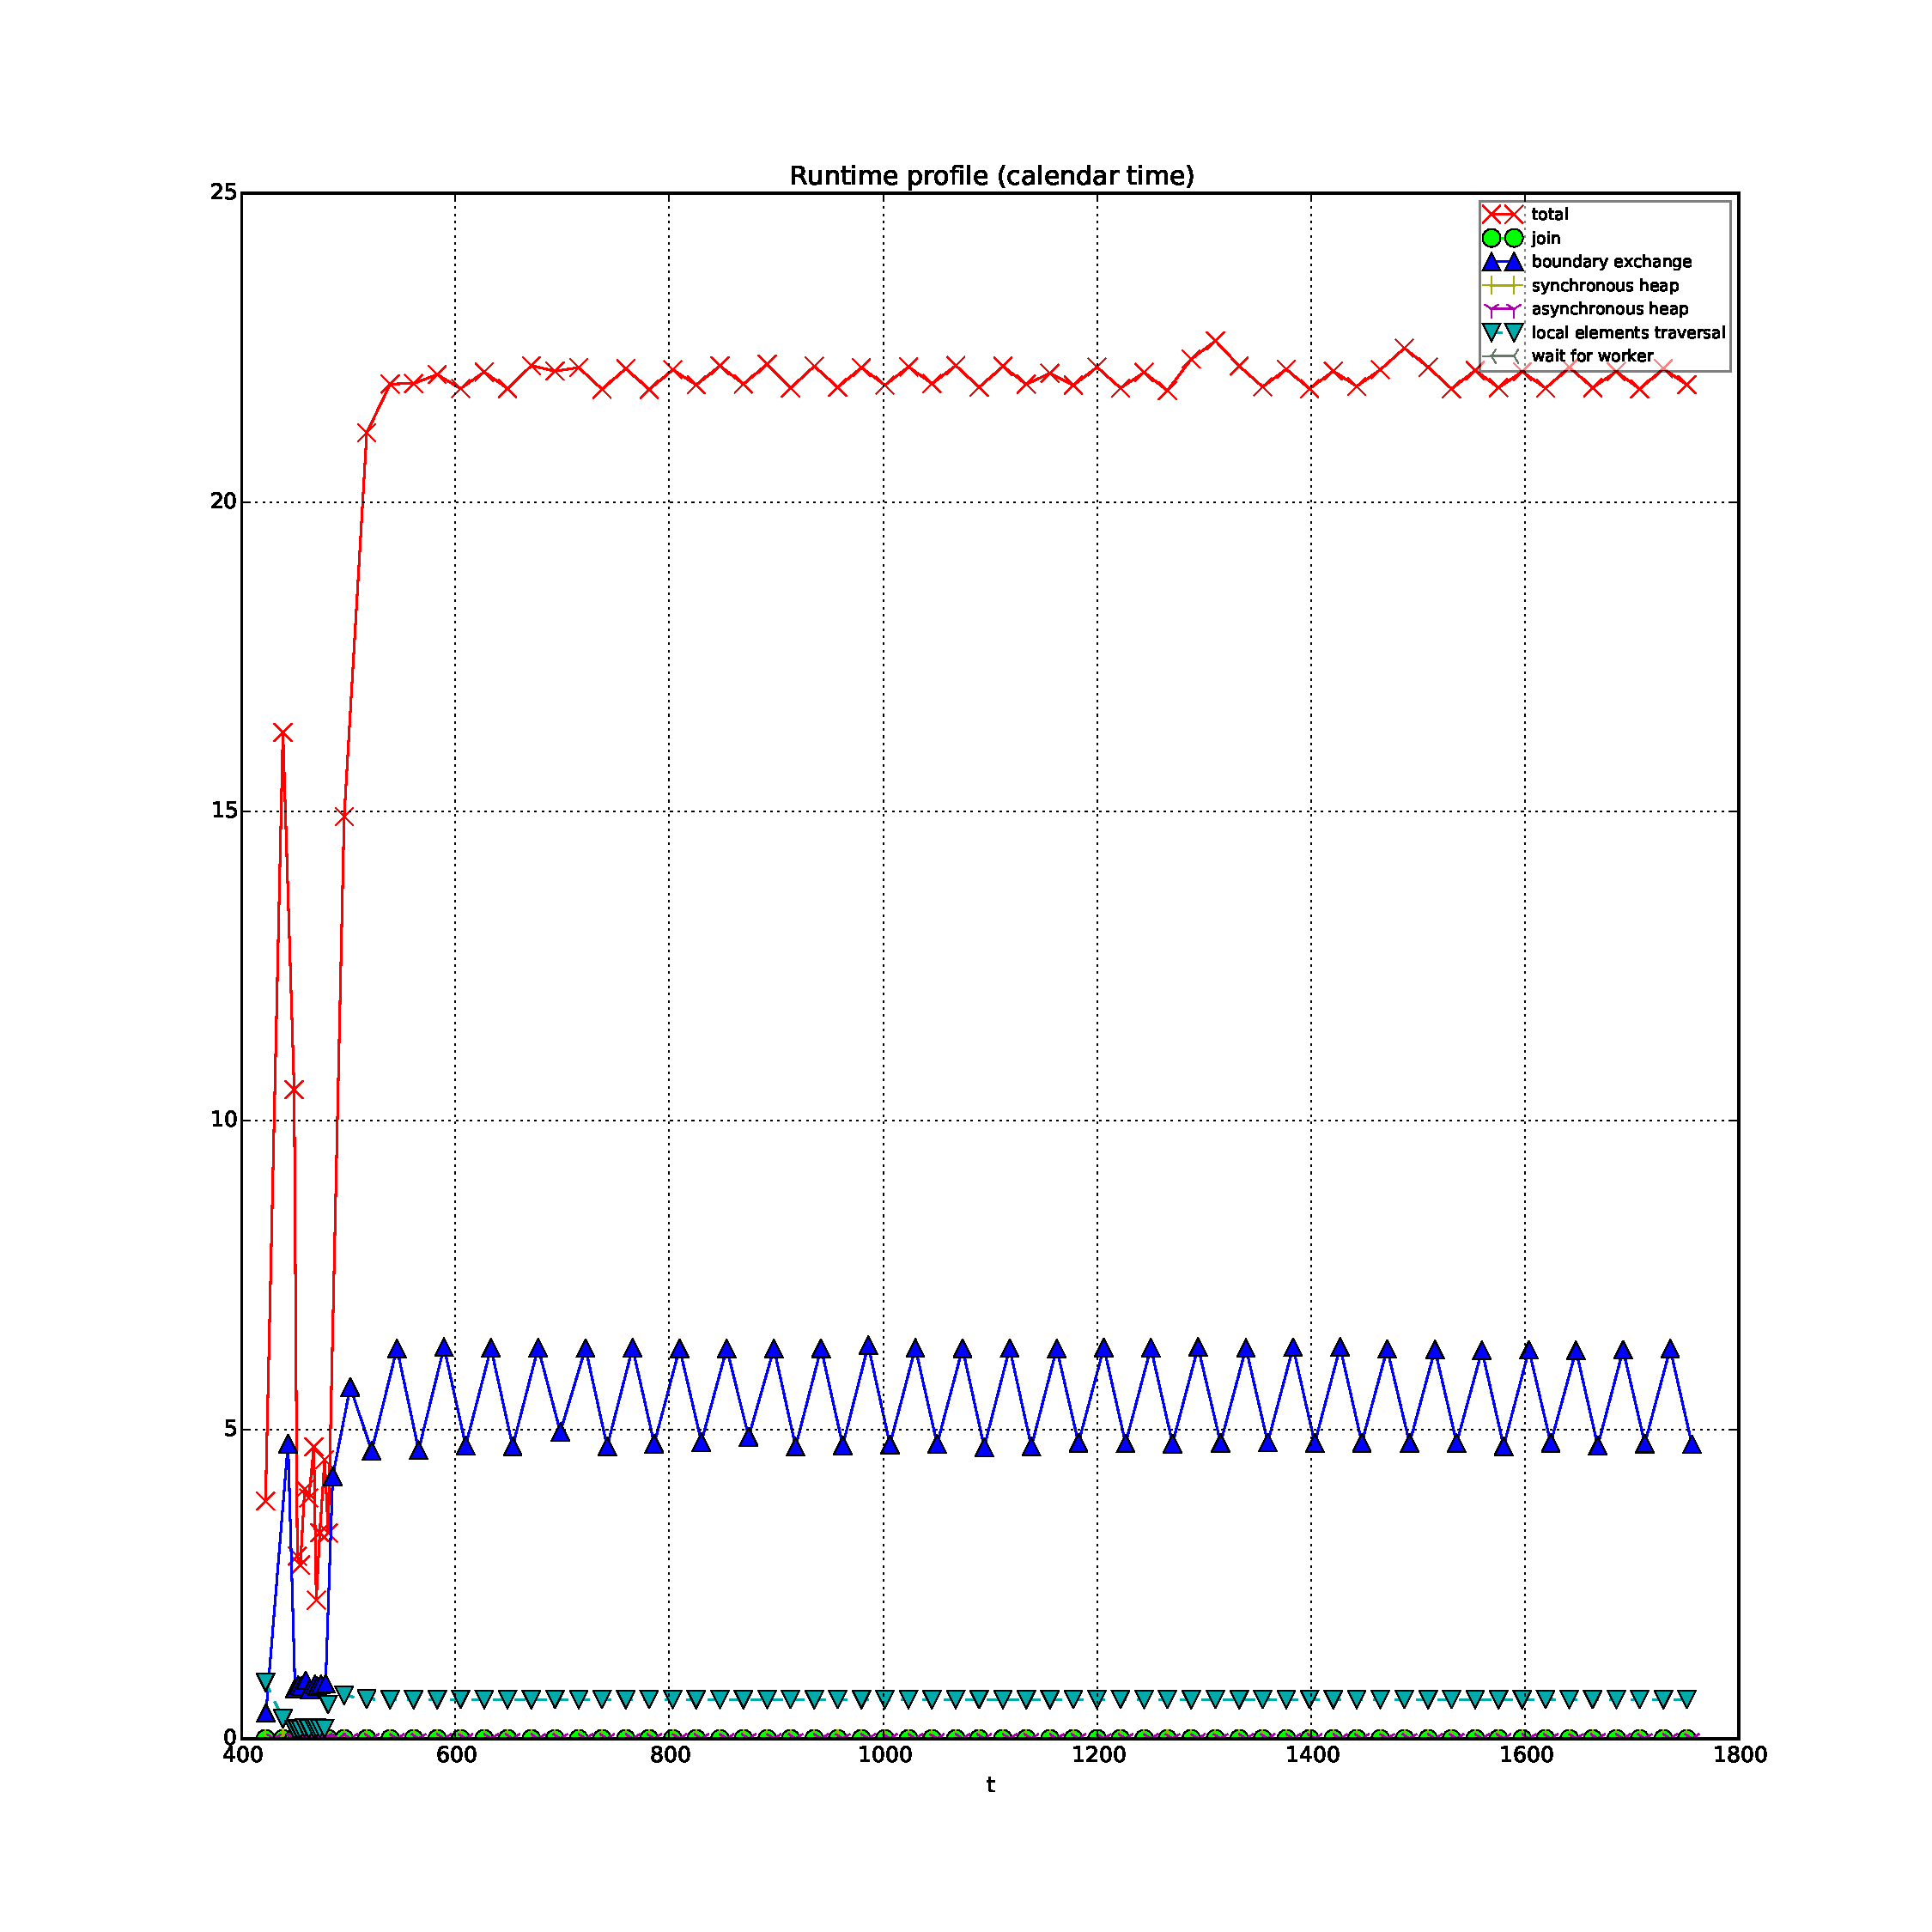
\includegraphics[width=0.5\textwidth]{64_advanced-mpi/boundary-exchange.pdf}
\end{center}


\noindent
We observe such a behaviour typically if the computational load per rank is low
(as we use low order finite elements, e.g.) or if all massive data exchange is
realised through heaps.
Heaps allow Peano to realise a more efficient data exchange than the standard
stack-based grid data, but they cannot communicate grid changes.

If we see such a pattern, it is worth to evaluate whether you can (temporarily)
switch off the data exchange and make the ranks work autonomously.
Peano passes control information along the MPI topology from masters to workers. 
We can switch off boundary data exchange on the first rank, i.e.~the global
master, and then this information is automatically propagated down to all the
ranks: all switch off the boundary exchange.

Peano realises a Jacobi-style boundary data exchange. 
Boundary data of one iteration is sent out throughout or, the latest, at the end
of the traversal.
Prior to the next traversal, this data is received. 
If we trigger a refine along a parallel boundary, this refine will thus become
active only in the subsequent iteration, when all ranks that hold a replicate of
the vertex have received copies of this vertex from all other ranks.
If we thus switch off the boundary data exchange, the next traversal still
receives vertices as they have been sent out the traversal before.
It however does not send out any data anymore.
In the second traversal (if we haven't switched on the boundary exchange again),
not data is exchanged anymore at all.
If we switch on the boundary data exchange again, the subsequent traversal sends
out grid data along the domain boundaries. 
Only in the second iteration after the switch on, both data is received and sent
out again.

While the description above claims that the boundary exchange control state is
exchanged via the state, we have to clarify that it is the repositories' state,
not the application-specific state. This is the state that also carries
information which adapter to run, e.g.
Therefore, the switch off is realised via the repository's \texttt{iterate}
command. 

\begin{code}
// on global master
const bool switchOffBoundaryExchange = true;
const int  numberOfIterationsToRunInOneRush = 10;
myRepository.iterate(numberOfIterationsToRunInOneRush,switchOffBoundaryExchange);
\end{code}

\noindent
The snippet runs one iteration where only boundary data is received but no
iteration is sent out anymore.
It then runs nine iterations where neither data is sent out nor received along
the boundary (from the grid; any heap data exchange is not affected).

Please note that the boundary data exchange is not switched off before you call 
\begin{code}
myRepository.iterate(...,false);
\end{code}
\noindent
once more. As soon as a \texttt{false} is passed, the subsequent first iteration
will not receive anything but send out boundary data. 
The iteration after, all communication, i.e.~both in and out, then is again
happening.



\begin{remark}
  If you switch off boundary data exchange, no load balancing can take place.
  Please also ensure that you switch off the exchange if and only if no
  rebalancing is going on, i.e.~the iteration before no rank has been joining or
  forking. 
  Otherwise, Peano will crash (with an assertion if compiled with asserts).
\end{remark}


\noindent
Peano does exchange vertices along the boundary after each grid sweep. 
It then compares all the refinement flags and performs the actual refinement.
This way, the grid remains consistent over all ranks: first, all refinement
information is exchanged. 
Once all ranks have received this information, the actual refinement is done.

If we switch off boundary exchange, obviously no refinement should ever be done
along domain boundaries as refinement triggers are not kept consistent.
Peano does switch off the refinement automatically, but you have to be aware how
a switch off of boundary information might affect your adaptivity patterns.

If a code triggers a refinement along a parallel domain boundary while
communication is switched off, this refinement does not pass through.
However, the refinement flag still is set. 
This means:
\begin{itemize}
  \item As soon as you reactive boundary data exchange, the code actually
  exchanges the refinement request. In the subsequent iteration, it then
  refines.
  \item The state remains instationary, i.e.~the state's \texttt{isGridBalanced}
  and \texttt{isGridStationary} return \texttt{false} as soon as the refinement
  is requested though it does not pass through.
\end{itemize}



\subsection{Further tuning}
This part has yet to be written, but I need documentation on 

\begin{itemize}
  \item \texttt{-DnoParallelExchangePackedRecordsAtBoundary}
  \item \texttt{-DnoParallelExchangePackedRecordsBetweenMasterAndWorker}
  \item \texttt{-DnoParallelExchangePackedRecordsInHeaps}
  \item \texttt{-DnoParallelExchangePackedRecordsThroughoutJoinsAndForks}
\end{itemize}

Dann gibt es auch noch die Flags

%

%Become topology-aware


% Throughout the bottom-up traversal, each mpi traversal first receives data from 
% all its children, i.e. data deployed to remote traversals, and afterward sends 
% data to its master in turn. Unfortunately, Peano has to do quite some 
% algorithmic work after the last children record has been received if and only 
% if some subtrees are also to be traversed locally. It hence might make sense to
% introduce pure administrative ranks that do not take over any computation on the finest grid level. 
% Again, we do a brief 1d toy case study:
% 
% foobar
% 
% In the upper case, the blue rank triggers the red one to traverse its subtree. The red one in turn tiggers 3 and 4. Afterward, it continues with 2 and then waits for 3 and 4 to finish. After the records from 3 and 4 have been received, it has to send its data to 0 to allow 0 to terminate the global traversal. However, between the last receive and the send, some administrative work has to be done, as the red node also holds local work (it has to run through the embedding cells to get the ordering of the boundary data exchange right, but that's irrelevant from a user point of view). This way, we've introduced an algorithmic latency: Some time elaps between 3 and 4 sending their data and the red one continuing with the data flow up the tree. This latency becomes severe for deep Splittings.


%   \newpage
%   \section{Tuning shared memory code}


\chapterDescription
  {
    Around 30 minutes.
  }
  {
    A working shared memory code.
  }


In this section, we discuss some aspects of shared memory parallelisation and
give some hints for proper shared memory parallelisation.


\subsection{Profiling}

Like any other optimisation, I do recommend to start with some profiling. This
should comprise the usage of proper profilers such as VTune Amplifier, but it
also should comprise at least one run where you
enable Peano's profiling outputs as discussed in
Section \ref{section:performance-analysis}.

Once you have obtained a program output with Peano's performance analysis
enabled, please pass this output to Peano's performance analysis scripts:
\begin{code}
python .../src/peano/performanceanalysis/performanceanalysisroutines.py
\end{code}
\noindent
Invoking the script without any argument displays some usage messages.


\begin{remark}
 Profiling Peano's shared memory behaviour induces a significant runtime
 overhead. Furthermore, it generates lots of code. As a result, Peano does some
 in-situ data accumulation. In return, it means that you have to run the code
 for a decent time and on decent problem sizes to get meaningful results.
 Otherwise, the accumulation does average out too many details.
\end{remark}


\begin{center}
 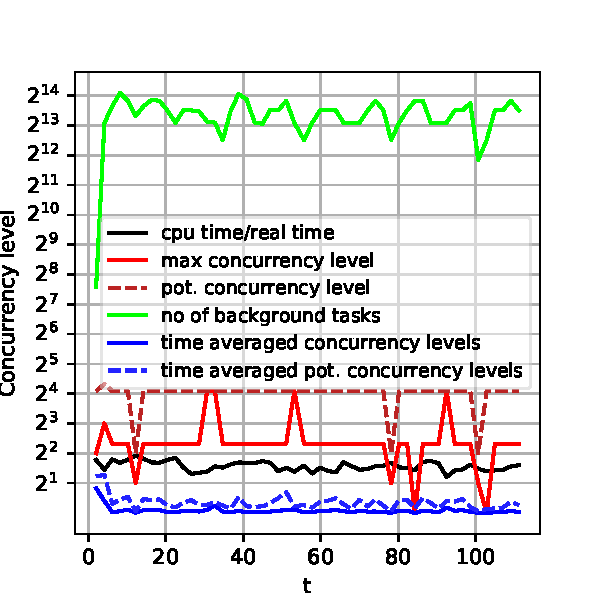
\includegraphics[width=0.6\textwidth]{67_shared-memory-tuning/trace-concurrency.pdf}
\end{center}

\noindent
Peano's shared memory profiling yields four different types of data.
These data stem from very small time sampling intervals. While the data is
sampled in small intervals, Peano dumps the aggregated data to the terminal only
every few seconds. As a result, data is noisy/smoothed out.
The data sets are coloured and we typically distinguish actual concurrency
behaviour to behaviour that could have been obtained if we had split up all
parallel codes into tiny little atomic tasks:

\begin{enumerate}
  \item The ``measured'' concurrency level is the cpu time burnt divided by the
  real time. Usually, this should be around the number of cores/threads you use
  as your system charges you for every physical thread.
  \item The maximum concurrency is the maximum number of threads that could have
  been idle over a small time interval. Peano works in terms of tasks. If the
  number of tasks exceeds the number of threads, the observed concurrency is
  smaller than the derived maximum concurrency. 
  \item The time averaged concurrency weights the individual subsamples averaged
  into one data dump with the underlying time spans, i.e.~it is something alike
  $\frac{\int _T f dt }{|T|}$.
  \item The number of background tasks tries to estimate how many background
  tasks are available at any given time. Peano does not realise a mechanism
  tracking the real number of background tasks, so this is a lower bound. There
  might be more tasks still pending in your system.
\end{enumerate}


\subsection{The measured concurrency level equals two}

\begin{smell}
 The measured concurrency level equals two no matter how many cores we try to
 use. Peano runs on a machine with more than one core.
\end{smell}

\noindent
As all cores today offer hyperthreading, we've ran into this smell when the
operating system/scheduler did mask/pin our code onto exactly one core. 
The code then uses the hyperthread, but cannot really scale beyond the core.
This is for example done by IBM's load balancer if you don't set the OpenMP
threads correctly---even if you don't use OpenMP but TBBs.

 
\subsection{Low concurrency levels}


\begin{smell}
 The (theoretical) concurrency level (black line) is very small. As a result,
 the obtained concurrency level is small, too.
\end{smell}

\noindent
There are multiple ways to tackle such a behaviour. Their ultimate goal is to
increase the concurrency of the code. However, you have to be careful: A
brilliant concurrency does not automatically mean that the code runs faster as
threads might be too small. So any optimisation here deserves a careful tracking
of total runtimes.

\begin{enumerate}
  \item Whenever Peano runs into a set of independent events such as
  \texttt{touchVertexFirstTime}, it does not automatically trigger them in
  parallel. Instead it first computes the cardinality of this set and then asks
  an oracle whether to process this set in parallel. The oracle not only says
  yes/no but also identifies well-suited grain sizes, i.e.~the minimal subset
  size. If you observe a low concurrency, it is a straightforward strategy to
  play around with the settings of the dummy oracle (if you use this one;
  cmp.~Section \ref{section:shared-memory:preparation}) or to use another oracle
  that is able to learn and to adopt the grain sizes automatically. You might also
  decide to write your own oracle.
  \item Whenever Peano runs into a set of (potentially) concurrent events, it
  evaluates the corresponding mapping specifications which concurrency
  constraints have to hold. Basically, they define in a colouring language
  (similar to red-black Gau\ss-Seidel) which events may run in parallel. If an
  adapter merges multiple events, the most restrictive constraint system
  dominates. If your overall concurrency level is too small, it is thus worth to
  study whether these constraint systems can be relaxed.
  \item Finally, you might decide to parallelise your own code within the
  mappings.
\end{enumerate}


\begin{remark}
  The mapping specifications are \textbf{not} static, i.e.~they can evaluate the
  mapping's state. In several projects, I found that some very restrictive
  colouring schemes are mandatory (in classic multigrid, I need often for
  example a $7^d$ colouring to ensure that no two vertices restrict their
  residual at the same time to a coarse vertex). However, they are not mandatory
  all the time, i.e.~I can make the specification query return a less
  restrictive pattern from time to time which speeds up the code significantly.
\end{remark}

\noindent
If you program your own code, you might want to use Peano's
\texttt{peano::grid::datatraversal::} \texttt{TaskSet} to split up your code
into multiple tasks. It then is independent of TBB/OpenMP. Furthermore, there's a macro
\texttt{pfor} in the \texttt{tarch/multicore} directory that allows you to write
parallel for loops that are again independent of the underlying shared memory
parallelisation scheme. A d-dimensional extension exists, too.

All of these helper functions again require a grain size which determines
whether and with which cardinality problems are to be split up.
You can use Peano's oracle mechanism here.
Whenever you ask the oracle for a grain size, you have to pass it the code
location.
Usually such a flag indicates some part of the grid management.
However, there's also a set of user-defined markers.
Use those (you have to bookkeep which ones you use where) to integrate into
Peano's oracle mechanism.

 
Here is an example from the ExaHyPE project where we use the tenth user-defined
marker:
\begin{code}
#include "tarch/multicore/Loop.h"

[...]

const int ProblemSize = ...;
auto grainSize = peano::datatraversal::autotuning::Oracle::getInstance().parallelise(
 ProblemSize,
 peano::datatraversal::autotuning::MethodTrace::UserDefined9
); 
// equals for(int i=0; i<ProblemSize; i++)
pfor(i, 0, ProblemSize, grainSize.getGrainSize())
  [...]
endpfor
grainSize.parallelSectionHasTerminated();
\end{code}



\subsection{Low time-averaged concurrency}

To identify/hunt down this issue, I strongly recommend that you switch off all
of your background tasks, i.e.~tasks you fire and later check for completion.
Tasks running independently in the background are a powerful tool to exploit
many cores, but they also tend to make performance data more difficult to
digest.
Furthermore, they help to exploit the cores but the core grid stuff usually
should already scale all alone without them, i.e.~they cannot compensate for a
poor grid concurrency.


\begin{smell}
  The time averaged concurrency is very small though both the maximum
  concurrency level and the cpu occupation (cpu time by real time) both exceed
  the core count. The code is not really fast.
\end{smell}

\noindent
The plot we are speaking about here are the blue lines. If they are small but
the black line approaches the number of cores, we have to assume that the code
consists of a lot of small tasks that are computationally very cheap.
While the code exploits the cores to process work concurrently, it spends quite
some time in administrating these tasks (scheduling) and running through serial
code parts that are sprinkled in between all the parallel code parts.
Furthermore, it might do quite some data consistency operations.


There is no siler bullet in this case, i.e.~if you can't increase the arithmetic
intensity significantly, you basically have to run through a series of trial and
error ideas without any guarantee of success:

\begin{enumerate}
  \item Peano internally realises a BSP-style data flow: Whenever the grid
  traversal runs into some section of the code that shall run in parallel, it
  copies all the mapping objects and triggers the parallel traversal. Once this
  traversal has terminated, it merges all the mappings again. Obviously, this is
  unneccessary overhead if the mappings' states do not change. In this case, we
  could omit the copying and the merging. To tell Peano to skip them, please set
  the last entry in the corresponding event specifications to \texttt{false}:
  \begin{code}
peano::MappingSpecification  
myprobject::mappings::MyMaping::ascendSpecification(int level) { 
 return peano::MappingSpecification(
  peano::MappingSpecification::Nop,
  peano::MappingSpecification::AvoidCoarseGridRaces,
  false // This false eliminates all the copying 
 );
}
  \end{code}
  In most of my own experiments, manipulating this flag howeve has only a very
  limited impact; often, it even backfires.
  \item Peano internally linearises the whole spacetree and, when it runs
  through the tree, reads on one data stream and pipes out the data stream for
  the subsequent iteration. There is an alternative storage scheme that is
  applies if a whole region of the grid remains stationary, is regular and the
  shared memory parallelisation tells the code to do so\footnote{The  design
  here is slightly flawed---a decision which storage format to choose has
  basically nothing to do with shared memory parallelisation. We hijack the
  shared memory decision making nevertheless as this storage decision starts to
  have its major influence once shared memory parallelisation is switched on.}.
  If you have a rather regular, starionary grid, you can doublecheck which
  storage format is chosen by letting \texttt{peano::grid} plot its stuff. You
  should obtain messages alike
  \begin{code}
  regular grid of height 5 used nonpersistently/persistently=0/1 times
  \end{code}
  and the index left of the \texttt{/} should be high(er). It depends on the
  type of shared memory oracle whether you can manually enforce a persistent
  storage. Please study the constructor's arguments.
\end{enumerate}


\begin{center}
 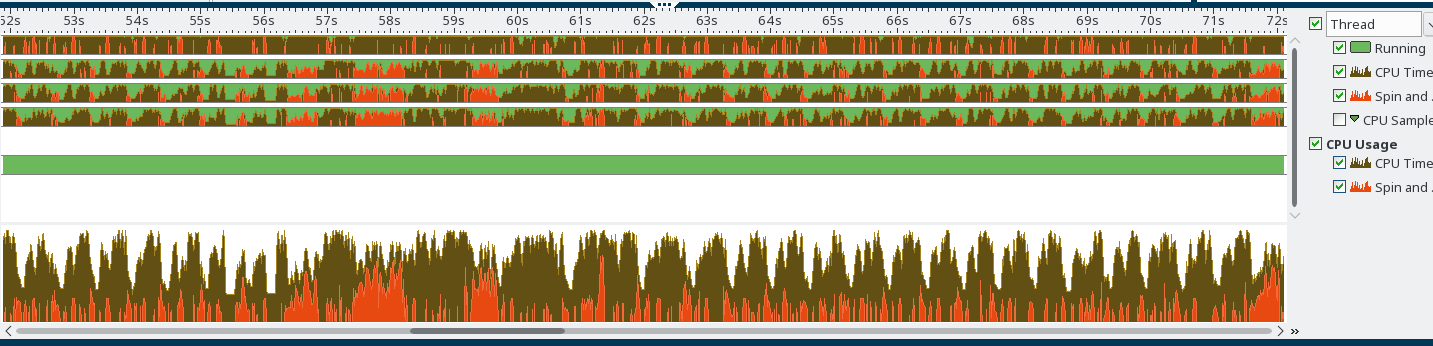
\includegraphics[width=0.8\textwidth]{67_shared-memory-tuning/vtune.png}
 \\
 {\footnotesize
  Typically VTune snapshot that uncovers very high spinning timings.  
 }
\end{center}

\begin{smell}
  The time averaged concurrency is very small though the code seems to exploit
  all cores. VTune complains about a lot of spinning.
\end{smell}

\noindent
There are basically two things you can do: 

\begin{enumerate}
  \item You can increase the grain sizes delivered by the shared memory oracles.
  If you use autotuning, this should automatically be done.
  \item If you use background tasks, try to fuse multiple of these tasks into
  a single one.
\end{enumerate}


\begin{center}
 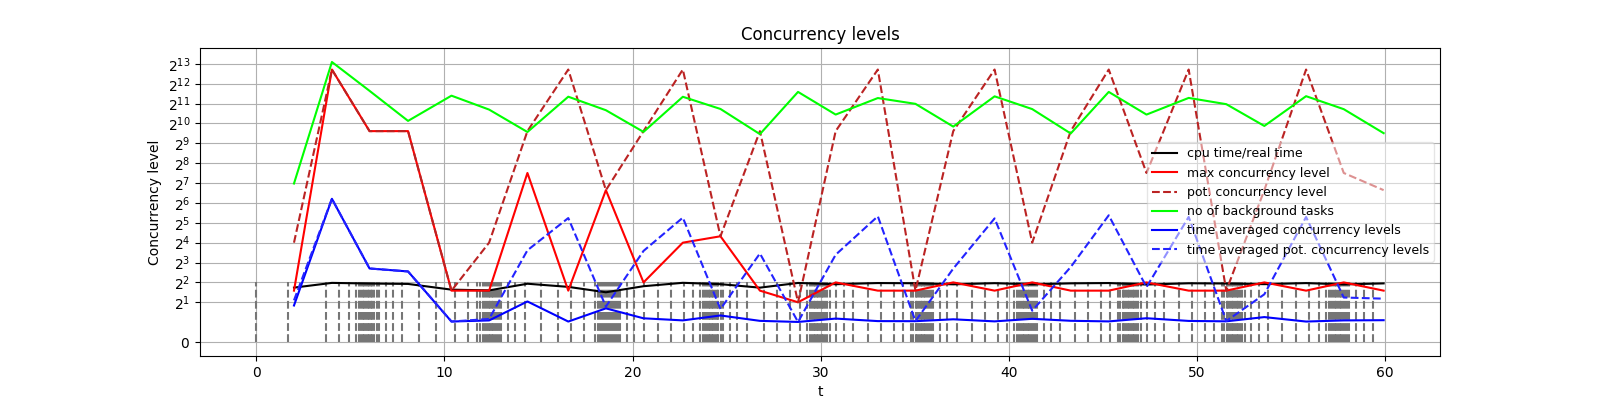
\includegraphics[width=0.8\textwidth]{67_shared-memory-tuning/concurrency.png}
 \\
 {\footnotesize
  Profile obtained through Peano's built-in profiling on a two-core laptop that
  shows that many background tasks would be available if there were more cores.
 }
\end{center}

%   \newpage
%   \section{Single core optimisation}

\chapterDescription
  {
    5 minutes.
  }
  {
  }


In this section, we discuss various aspects tied to alignment and vectorisation. 


\subsection{Vectorisation of basic linear algebra}

Peano does come along with its own small technical architecture (\texttt{tarch})
that holds some basic linear algebra routines. These routines currently are
vectorised via Intel's SIMD pragmas. The pragmas are active if and only if the
define \texttt{CompilerICC} is set. 

All linear algebra routines (and various other parts of the code) include the
file \linebreak
\texttt{tarch/compiler/CompilerSpecificSettings.h}.
This header evaluates various compiler predefines and tries to identify on which
machine you compile.
It then includes a compiler-specific include file which sets flags alike 
\texttt{CompilerICC} if an Intel compiler is found.

For cross-compilation or tuning of your settings, it might be reasonable to
either adopt the spec file or to write your own header file which
defines/undefines certain compiler settings.


\subsection{Alignment of heap data}

Most codes managing larger double arrays within Peano use Peano's heap to do so. 
By default, the heap relies on the \texttt{std::vector} class and its embedded 
plain C++ array. 
By default, heap data is not aligned.


For the heaps hosting doubles, Peano however offers aligned variants. See the
file \linebreak
\texttt{peano/heap/DoubleHeap.h} for examples. 
There are a few predefined (typedefs) heaps, but you might want to define your
own.


Once you use the aligned heaps for your \texttt{double} data, its interface
provides you access to standard C++ \texttt{std::vector<double>} objects.
These objects have a \texttt{data()} operation through which you can get a 
pointer to an aligned double array.

\begin{code}
typedef peano::heap::RLEDoubleHeapAlignment64  MyDoubleHeap;

double* x = MyDoubleHeap::getInstance().getData(myIndex).data();

// x is now aligned to 64 bytes.
\end{code}


% Alle Optionen von PeanoOptimisations.h durchgehen
%
%

%Become topology-aware


% Throughout the bottom-up traversal, each mpi traversal first receives data from 
% all its children, i.e. data deployed to remote traversals, and afterward sends 
% data to its master in turn. Unfortunately, Peano has to do quite some 
% algorithmic work after the last children record has been received if and only 
% if some subtrees are also to be traversed locally. It hence might make sense to
% introduce pure administrative ranks that do not take over any computation on the finest grid level. 
% Again, we do a brief 1d toy case study:
% 
% foobar
% 
% In the upper case, the blue rank triggers the red one to traverse its subtree. The red one in turn tiggers 3 and 4. Afterward, it continues with 2 and then waits for 3 and 4 to finish. After the records from 3 and 4 have been received, it has to send its data to 0 to allow 0 to terminate the global traversal. However, between the last receive and the send, some administrative work has to be done, as the red node also holds local work (it has to run through the embedding cells to get the ordering of the boundary data exchange right, but that's irrelevant from a user point of view). This way, we've introduced an algorithmic latency: Some time elaps between 3 and 4 sending their data and the red one continuing with the data flow up the tree. This latency becomes severe for deep Splittings.


%   \newpage
%   \section{Compiler-based optimisation}

\chapterDescription
  {
    5 minutes
  }
  {
  }


Peano's implementation can be tailed by tons of different compile options. 
At the end of the day, one might have to tailor them on a per-project base. 
As the settings first of all are tied to a particular machine (besides an
application), Peano collects all magic variables within a file called
{\em CompilerSpecificSettings.h}.
For some default platforms, we provide meaningful results.
All of these settings however can be overwritten no the command line.


\subsection*{Single core}

\begin{center}
 \begin{tabular}{p{2cm}p{2cm}p{9.5cm}}
  Compile flag (default) & Alternative & Description \\
  \hline
  {\footnotesize Use\-Manual\-Inlining} 
  & 
  {\footnotesize noUse\-Manual\-Inlining} 
  &
  Compilers are known to implement good heuristics which routines to inline and
  which not to inline. We however found that some compiler struggle with some
  parts of Peano. For these parts, we have added compiler-specific annotations
  that force the compiler to inline. Obviously, the identification of critical
  code parts has been done for few benchmarks only and it might happen that they 
  are invalid or even contra-productive for some applications. 
  \\
  \hline
 \end{tabular}
\end{center}
  

\subsection*{Shared memory}

\begin{center}
 \begin{tabular}{p{2cm}p{2cm}p{8cm}l}
  Compile flag (default) & Alternative & Description & Target \\
  \hline
  {\footnotesize UseTBBs\-Parallel\-For\-And\-Reduce} 
  & 
  {\footnotesize noUse\-TBBs\-Parallel\-For\-And\-Reduce} 
  &
  Different to TBB, Peano's internal task/job system literally is based on
  tasks only. That is, also parallel loops are mapped onto job spawning. For
  TBB-based codes, we found that such a realisation is sometimes disadvantageous
  for larger core counts. The flag allows us to toggle the implementation. 
  & TBB
  \\
  \hline
 \end{tabular}
\end{center}
  
  
  
\subsection*{Distributed memory}

\begin{center}
 \begin{tabular}{p{2cm}p{2cm}p{9.5cm}l}
  Compile flag (default) & Alternative & Description \\
  \hline
  {\footnotesize MPI\-Progression\-Relies\-On\-MPI\-Test} 
  & 
  {\footnotesize noMPI\-Progression\-Relies\-On\-MPI\-Test} 
  &
  Some MPI implementations struggle to transfer data in the background of the
  simulation run. In this case, one has to call \texttt{MPI\_Test} over an over
  again. Each test call allows MPI to progress some messages. Obviously,
  these calls do not come for free and impose some overhead, too. The flag
  allows users to disable/enable this test polling. Unless not pinned
  explicitly to one thread (see below), Peano's hybrid implementation
  distributes the tests to the cores, i.e.~hardware threads call 
  \texttt{MPI\_Test} whenever they become idle.
  \\
  \hline
 \end{tabular}
\end{center}


\noindent
No following variables are by default set to 0. 
  
  
%            /**
%           * @param communicateSleep -1 Data exchange through blocking mpi
%           * @param communicateSleep  0 Data exchange through non-blocking mpi, i.e. pending messages are received via polling until MPI_Test succeeds
%           * @param communicateSleep >0 Same as 0 but in addition, each unsuccessful MPI_Test is follows by an usleep
%           */
  
  
%   #ifndef SendWorkerMasterMessagesBlocking
%  #define SendWorkerMasterMessagesBlocking     0
% #endif
% #ifndef SendMasterWorkerMessagesBlocking
%  #define SendMasterWorkerMessagesBlocking     0
% #endif
% #ifndef ReceiveMasterMessagesBlocking
%  #define ReceiveMasterMessagesBlocking        0
% #endif
% #ifndef SendAndReceiveLoadBalancingMessagesBlocking
%  #define SendAndReceiveLoadBalancingMessagesBlocking    0
% #endif
% #ifndef ReceiveIterationControlMessagesBlocking
%  #define ReceiveIterationControlMessagesBlocking        0
% #endif
% #ifndef BroadcastToIdleNodesBlocking
%  #define BroadcastToIdleNodesBlocking                   0
% #endif
% #ifndef BroadcastToWorkingNodesBlocking
%  #define BroadcastToWorkingNodesBlocking                0
% #endif
% #ifndef SendHeapMetaDataBlocking
%  #define SendHeapMetaDataBlocking                       0
% #endif
% #ifndef SendAndReceiveHeapSynchronousDataBlocking
%  #define SendAndReceiveHeapSynchronousDataBlocking      0
% #endif
%   
\subsection*{MPI+X}

\begin{center}
 \begin{tabular}{p{2cm}p{2cm}p{8cm}l}
  Compile flag (default) & Alternative & Description & Target \\
  \hline
%   {\footnotesize MPI\-Progression\-Relies\-On\-MPI\-Test} 
%   & 
%   {\footnotesize noMPI\-Progression\-Relies\-On\-MPI\-Test} 
%   &
%   Some MPI implementations struggle to transfer data in the background of the
%   simulation run. In this case, one has to call \texttt{MPI\_Test} over an over
%   again. Each test call allows MPI to progress some messages. Obviously,
%   these calls do not come for free and impose some overhead, too. The flag
%   allows users to disable/enable this test polling. Unless not pinned
%   explicitly to one thread (see below), Peano's hybrid implementation
%   distributes the tests to the cores, i.e.~hardware threads call 
%   \texttt{MPI\_Test} whenever they become idle.
%   & MPI
  \\
  \hline
 \end{tabular}
\end{center}

%

\noindent
Please note that all parameters are written without hyphens, i.e.~a parameter
alike \texttt{noTrippleX} which is written as no-Tripple-X in the table above is
switched on on the compiler level through \texttt{-DTrippleX} and disabled
through \texttt{-DnoTrippleX}.





%  
%

 \part{Design decisions}
 \newpage
 \chapter{Domain decomposition and data flow}
\label{section:design:domain-decomposition}

\Peano\ starts from spacetrees and thinks in whole trees and only supports two
types of decomposition operations: a split and a join.
At the same time, it does not distinguish shared memory and distributed memory
parallelisation.
It only thinks in terms of trees.
The trees and their traversal can either be deployed to ranks or threads or
combinations of the two.


This statement is only weakened once you work with \Peano's task interface. 
If trees issue tasks, then these tasks team up with the tasks handling the
individual spacetrees.
Your task graph starts to contain a mixture of tree tasks and user-defined
tasks.
This section discusses solely the tree decomposition aspect within \Peano.


\Peano\ relies on a multiscale non-overlapping domain decomposition. 
Within the trees, we distinguish three different types of parallel data flow:
\begin{itemize}
  \item {\bf Horizontal data exchange} is exchange between two cells of one
  level along their boundary.
  \item {\bf Vertical data exchange} is exchange between trees where one
  resolution meets the other. Vertical data exchange is also used to stream
  data from one rank to the other if we fork. Joins do not stream logically.
\end{itemize}



\section{Multigrid topology}

A tree in Peano is split along the Peano space-filing curve.
This implies that the decomposition of the finest mesh is a non-overlapping
decomposition where each cell is assigned to exactly one rank.
I use rank as term for rank or thread or task. 
See the discussion above.


Also Peano's coarser cells are uniquely assigned to one tree. 
Between the ranks, we have a tree topology again. 
That is, a splitting of a tree is always realised such that there's a unique
master-worker topology.

\begin{figure}
  \begin{center}
    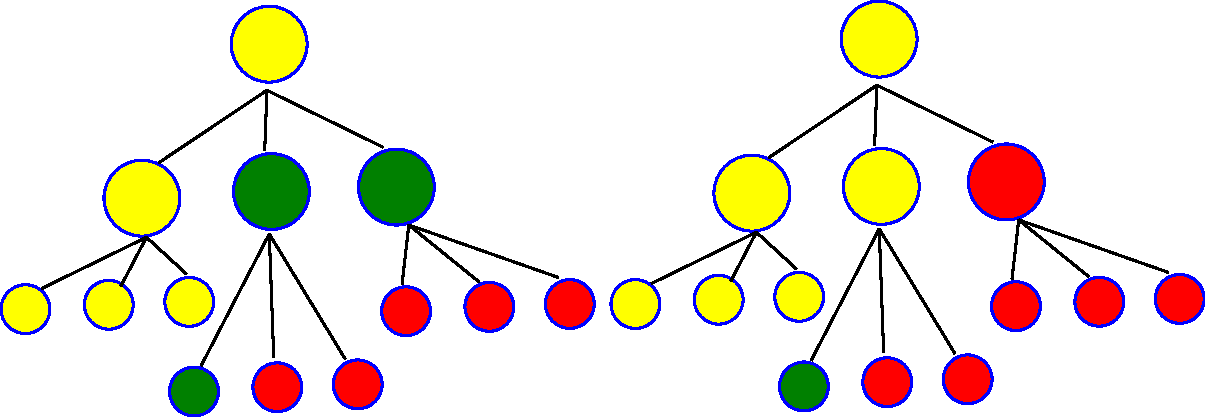
\includegraphics[width=0.8\textwidth]{51_domain-decomposition/tree-topology.pdf}
  \end{center}
  \caption{
    Two examples of a tree decomposition.
    \label{figure:51_domain-decomposition:tree-topology}
  }
\end{figure}

Some examples in Figure \ref{figure:51_domain-decomposition:tree-topology}
sketch the implications:
In the left example, the yellow tree has split up into yellow and green. The
green tree has further split into green and red.
The code usually tries to keep whole trees, i.e.~children and parents, within
one tree.
In the left example, it would be natural to make the very right green cell on
the first child level a red one, too.
This way, a whole tree would reside in red.
However, if we made this single cell red, then red would become a child of
yellow, i.e.~we would change the rank topology.
Peano never does so.

In the right example conversely, I've asked the yellow tree to split into
yellow, green and red in one rush. 
This time, the right level 1 cell becomes red already. 

Both examples show that a split of one tree into $n$ trees never
results in the fact that the original tree becomes empty.
Otherwise, we woudl again change the tree topology upon the ranks.


\section{Data flow on stationary domains}

\subsection{Horizontal data flow}

\Peano\ uses a non-overlapping domain decomposition.
Therefore, ie shares/exchanges faces and vertices between different trees.
It never shares cells of one level.
I explain the code's data exchange pattern with vertices.
Yet, the same pattern holds for faces, too.
After a code has read/written a vertex for the very last time throughout a
traversal, it sends a copy of this vertex away.
In-between two iterations, all trees exchange their data.
That is, in the next iteration any sent out data is available on the destination
rank and can be merged into the local data structures.
This merge happens on the destination prior to any other operation.


\begin{center}
 \includegraphics[width=0.5\textwidth]{51_domain-decomposition/boundary-data-flow.pdf}
\end{center}

\noindent
\Peano\ consequently realises a data exchange that is similar to Jacobi
smoothers:
Whatever you do on one tree won't be visible on the other trees in this very
tree traversal.
Prior to the next tree sweep, this information however becomes available there.


\subsection{Vertical data flow}

This yet has to be written.

\subsection{Synchronous vertical data flow}

This yet has to be written.


\section{Splits}

Whenever you split a tree, Peano creates the new trees (either as threads on
the local node or remotely via MPI). 
Each new tree receives a whole copy of the original tree. 
This is only tree data. 
User data is handled separetely.
Once the tree is replicated, the individual trees start to coarsen.
If they are not responsible for tree parts, they successively remove this part. 
After one or two iterations, each rank thus really works only on local tree.


\begin{remark}
 Peano uses information from the actively used data to decide which data to
 replicate.
 If you have cell and vertex and face data but you use some of these data only
 in some substeps of you algorithm, please ensure that those steps that trigger
 the domain decomposition and those that run immediately after this do use all
 data types.
 Otherwise, Peano can't know what data is to be replicated when it splits trees.
\end{remark}


\subsection{Temporal ordering of tree traversals}

With the information of the data flow above, any splits actually has to be
realised over two grid sweeps which internally decompose into substeps:

\begin{enumerate}
  \item The user asks a tree to split. From hereon, we have a master with some
  neighbours and a worker. The latter does not physically exist yet.
  \item The master runs through its domain and tells all neighbouring ranks that
  the new tree will drop in in the future. At this time, these neighbours are
  not yet aware of the split (the information becomes only available in the
  subsequent iteration), so they continue to send their stuff to the master even
  though it might be vertices which will, in the future, belong to the new
  worker. We say that that we have a {\bf split-triggered} in this iteration.
  \item In the next iteration, the master is {\bf splitting}. It still holds the
  ownership of all the data, as it receives for example all neighbour data.
  However, in the splitting phase, the master already sends out data to the
  worker where new domain boundaries will arise---even though the new worker
  does not exist yet. The same happens to all the neighbours. They send out
  boundary data to this new worker that will now enter the game.
  \item Once the master has terminated, the responsible rank issues a couple of
  postprocessing steps:
  \begin{enumerate}
    \item It clones the whole master tree. This is only the grid structure, but
    it is a complete clone.
    \item It instantiates the new worker with this cloned data. As we clone
    after the master's traversal has terminated, a lot of trees have already
    sent data to the new worker that we just cloned. However, this worker has
    not yet sent out any data, so we've broken the symmetry of our data
    exchange. Therefore, we run through the tree once as {\bf empty tree}. In
    this sweep, we do nothing. We only run once through the tree to ensure
    that the stack data is in the right order.
    \item Immediately after that, we do a {\bf new tree} sweep. This sweep does
    not invoke any user events. It however sends out the data the others expect
    from us.
  \end{enumerate}
\end{enumerate}


\begin{center}
 \includegraphics[width=0.35\textwidth]{51_domain-decomposition/split-data-flow.pdf}
\end{center}





\subsection{User data}

This has yet to be written.




\section{Joins}


The join of partitions in \Peano\ follows a few mantraic principles:

\begin{enumerate}
  \item We only join partitions if they do not hold refined cells. We call such
  partitions deteriorated (in a tree sense). If a partition holds a refined cell,
  it cannot be merged into its father.
  \item We hide joins from the user, i.e.~a user can split up a partition and
  thus implement load balancing, but a user is never allowed to join. Joins are
  always triggered by \Peano's core internally. The policy is as follows:
  \begin{itemize}
    \item We join a deteriorated partition if the master resides on the same rank
    and if this master would like to coarsen its domain but can't do so as this
    coarsening would violate the tree topology (see dicussion above).
    \item We join a deteriorated partition if the master resides on a different
    rank. The idea here is that such deteriorated partitions always induce quite
    some overhead.
  \end{itemize}
\end{enumerate}


\noindent
There's technical rationale behind some items:
We don't join deep trees with their master as both master and worker work with
their LET, i.e.~try to coarsen their respective mesh as aggressively as possible
after the split.
Therefore, a master does not have all grid infrastructure of a worker available.
It would require some complex zipping to bring the info of two trees together.
If I realise a deteriorated-trees-only policy, I don't need such zipping as
(almost) all information is available on the master already.



\subsection{Grid data streaming}


In principle, one might assume that no streaming is required if we merge only
deteriorated trees. 
After all, if a rank deploys some subtree to another worker, it still holds its
root node locally (though flagged as remote).
However, there's one delicate special case:
If a tree joins its master and another neighbour changes something within the
mesh, too (merges as well or splits up), then the master won't be notified of
this info.
The update information will reach the worker while it is joining into its
master.
Therefore, a merging worker does stream its vertex data immediately into the
master while it joins.
This streaming requires us to break up the join process into two distinct
traversal phases (see primary vs.~secondary remark above).


Hijack vertical stacks on grid side!


\marginpar{Rework}

Joins are completely hidden from the user, i.e.~there's no way to actively join
trees. 
To understand why Peano issues joins from time to time, it is important to
define vetoed coarsening.

\begin{definition}
 Peano vetos any coarsening, if removing some parts of the grid would affect a
 child or alter the tree topology of the ranks.
 If a coarsening is vetoed, Peano remembers this veto. 
 As soon as a rank whose master is affected by a veto hosts a tree cell which is
 unrefined, it joins/merges this cell into the master.
\end{definition}

\noindent
Vetoed coarsening typically does delay any grid coarsening.
You ask for a coarsened grid, and it first of all applies this coarsening to all
ranks that have not decomposed further.
Once these have finished their coarsening, it joins those ranks that stop
further coarsening into their master.
Once this is complete, it continues to coarsen.
This process can continue recursively.


\section{Data flow}


\section{Grid entity markers}

As pointed out above, Peano works with replica of trees and then removes per
rank those grid entites which are not adjacent to the local domain.
This implies that some cells plus their data are held redundantly.

Whenever Peano invokes an activitiy on a grid entity, it passes a marker besides
the actual data.
Markers typically hold spatial information.
In a parallel run, a marker also tells you whether the cell or vertex currently
handled is a local one, adjacent to the domain boundary, or overlaps into a
neighbouring domain which actually holds it.



%60_exahype.tex


 \part{Standard benchmarks}
 \newpage
 \chapter{Benchmark: Task priorities}
\label{chapter:benchmark:task-priorities}


This benchmark has been written as part of the Sheffield GPU Hackathon sponsored
by NVIDIA where we took part with the ExCALIBUR project ExaClaw.
It assesses whether the task realisation (incl.~priorities) is appropriate for
\Peano\ and \ExaHyPE.
That is, we have used this benchmark to uncover weaknesses in the OpenMP and TBB
backbone of \Peano\ as well as our layer on top to connect to these libraries.
The benchmark uses \ExaHyPE's Euler equation implementation in 2d.

\begin{center}
 \includegraphics[width=0.16\textwidth]{logos/EU.pdf}
 \includegraphics[width=0.2\textwidth]{logos/ExaHyPE-logo.png}
 \includegraphics[width=0.2\textwidth]{logos/excalibur.png}
 \includegraphics[width=0.2\textwidth]{logos/GPUHackathon-white-logo.png}
\end{center}


\section{Preparation}

Download \Peano\ (branch p4) and configure the code with \ExaHyPE\ support.
Choose the multithreading backend of your choice.
Depending on your system, I recommend you activate an appropriate tracing.
\Peano\ supports at least support for ITAC (Intel) 

\begin{code}
 ./configure --
\end{code}

\noindent
and NVTX (NVIDIA):

\begin{code}
 ./configure --enable-exahype --with-multithreading=omp --with-nvidia \
   CXXFLAGS=-DUseLogService=NVTXLogger
\end{code}

\noindent
All of the above examples ignore that you might have to set the appropriate
compiler (\texttt{CXXFLAGS}) and linker (\texttt{LDFLAGS}) flags as well such
that the build systems finds all required include and library files.
In particular, your \texttt{LDFLAGS} have to link to \texttt{-lnvToolsExt}.


Build the code.


\section{Set up the experiment}

Change into the examples directory hosting the Euler solver.
We rely on \Peano's Python API here:

\begin{code}
cd python/examples/exahype2/euler
\end{code}

\noindent
For the benchmark, we rely on a simple Euler setup working with a regular grid.
However, we use enclave tasking, i.e.~the task production pattern is
nevertheless already reasonably complex.
We run the code for ten iterations on a rather smallish grid:

\begin{code}
import os
import peano4
import peano4.datamodel
import peano4.solversteps

import exahype2

#
# Create a project and configure it to end up in a subnamespace (and thus
# subdirectory). 
#
project = exahype2.Project( ["examples", "exahype2", "euler"], "finitevolumes", "." )

#
# Add the Finite Volumes solver
#
patch_size     = 7
unknowns       = 5
time_step_size = 0.000001
volume_max     = 0.03
project.add_solver(  exahype2.solvers.GenericRusanovFVFixedTimeStepSizeWithEnclaves(
  "Euler", 
  patch_size, 
  unknowns, time_step_size,
  flux = True,
  ncp  = False
))


#
# Lets configure some global parameters
#
dimensions = 3
build_mode = peano4.output.CompileMode.Trace
project.set_global_simulation_parameters(
  dimensions, [0.0,0.0,0.0], [1.0,1.0,1.0],
  time_step_size * 10,           # end time
  0.0, 0                         # snapshots
)


#
# Add parallelisation
#
project.set_load_balancing( "toolbox::loadbalancing::RecursiveSubdivision" )

peano4_project = project.generate_Peano4_project()
peano4_project.constants.export( "MaxHOfVolume", volume_max )
peano4_project.output.makefile.parse_configure_script_outcome( "../../../.." )
peano4_project.output.makefile.add_library( project.get_core_library(build_mode), 
 "../../../../src/exahype2" )
peano4_project.output.makefile.add_library( "ToolboxLoadBalancing" + 
 project.get_library_postfix(build_mode),
 "../../../../src/toolbox/loadbalancing" )
peano4_project.output.makefile.set_mode(build_mode)
peano4_project.build(make_clean_first=True)
\end{code}

\noindent
The important bit here, compared to other experiments, is that you use the
tracing target.
After you have passed this config file through the Python frontend, ensure that
you have a \texttt{exahype.log-filter} file in your work directory.
It should contain at least the following statements:

\begin{code}
info tarch    -1 white
info peano4   -1 white
info examples -1 white
info exahype2 -1 white
info toolbox  -1 white

trace tarch    -1 black
trace peano4   -1 black
trace examples -1 black
trace exahype2 -1 white
trace toolbox  -1 black

trace exahype2::fv -1 black
trace peano4::parallel::SpacetreeSet -1 white
\end{code}



\section{Run the code}

Run the code without any further arguments 
\begin{code}
./peano4
\end{code}

\noindent
The command line output (it differs depending on which command line logger you
have chosen) should tell you that you have
\begin{itemize}
  \item 729 cells in total, each one hosting a patch of $7 \times 7 \times 7$
  finite volumes;
  \item These cells are split up into four segments. The default splitting
  should be something similar to 81, 216, 216, 216 cells. That means the
  partitioning is not very good.
  \item We have in total 1485 cells, i.e.~the setup suffers from a high number
  of outer cells that do not carry any information.
\end{itemize}


\section{Visualise the outcome}

\begin{center}
 \includegraphics[width=0.9\textwidth]{21_task-priorities/nsight.png}
\end{center}

\noindent
The above illustration is an illustration with NVIDIA Nsight Systems 2020.3.1.
The code did nine time steps, and each time step consists of two grid sweeps. 
We see this pattern clearly in the last thread. 
We also see that this decomposition is ill-balanced, as two threads are very
busy all the time, one is reasonably busy, and one faces quite some idle time.
This setup is ill-balanced and the task distribution does not work as it should
be.

\begin{center}
 \includegraphics[width=0.9\textwidth]{21_task-priorities/zoom-in.png}
\end{center}


\noindent
A zoom-in (remember that two blackish bars above represent one time step)
reveals that the majority of enclave tasks is handled on the first thread which
is the slowest ones.
These are the dark grey bars in the illustration below.



\subsection{What we should see}

\Peano\ splits up each time step into two mesh traversals.
Each mesh traversal runs through one of the (four) subdomains as introduced
above. 
The first traversal runs through the mesh and issues a lot of tasks.
It also solves some Finite Volume problems and issues the MPI messages (not
relevant here).
The tasks should go into the background, as they are low priority (background
tasks).
This first traversal is ill-balanced, as the mesh decomposition is slightly
ill-balanced.


In the second traversal, each thread runs again through its domain.
This time, it waits per cell for which we have issued a background task before
until its task is done.
Throughout this wait, it processes some of the tasks.
The traversals per se again are ill-balanced. 


What we should see is that three out of four traversals needs pretty much the
same time, as the grid is decomposed into three big chunks plus one smaller one.
We should also see that the background tasks (dark items) slot into the idle
time of the briefer task.


\subsection{Data flow spec}

The underlying code is realised as follows (this is a generic pattern that I
use for all implementation backends):

\begin{enumerate}
  \item The code runs through the domain parts with a big parallel for.
  \item The parallel fors spawn background tasks. They can either be real tasks
  (with low priority) or we enqueue them manually into a task container.
  \item The code issues tells the task system once that it has finished its
  traversal (see below).
  \item The code runs through the domain parts once more with a big parallel
  for.
  \item Per cell, it checks whether it has spawned a task before and whether
  this task outcome is already there.
  \item If the task is not there, the traversal processes one task from the
  background queue (it could also yield) and checks again, i.e.~the checks
  realise (logically) some kind of busy polling.
\end{enumerate}


\subsection{Code regions causing the behaviour}

All code that leads to the discussed behaviour can be found in
\texttt{src/tarch/multicore/tbb/Tasks.cpp} or
\texttt{src/tarch/multicore/omp/Tasks.cpp}, respectively.
The routine that is responsible for the parallel mesh run-through (grid
traversals) is called \texttt{tarch::multicore::spawnAndWait()}.


The handling of the parallel tasks is done in
\texttt{tarch::multicore::processPendingTasks()} which each traversal calls
\begin{itemize}
  \item once after it has finished its local traversal (with the parameter 0 to
  indicate that it is not waiting for anything but it might be a good idea go
  launch some task progression threads);
  \item every time the code waits for a background task outcome (with the
  parameter 1, as it says ``do one task and return so I can check whether the
  result I'm waiting for meanwhile has dropped in'').
\end{itemize}


\section{Flaws identified}


\subsection{OpenMP: task group}

I have used a simple OpenMP task group
\begin{code}
void tarch::multicore::spawnAndWait(
  const std::vector< Task* >&  tasks
) {
  #pragma omp taskgroup
  for (int i=1; i<tasks.size(); i++) {
    #pragma omp task
    {
      while (tasks[i]->run()) {}
      delete tasks[i];
    }
  }
}
\end{code}

\noindent
It seems that this snippet uses five threads for four subpartitions. 



\subsection{OpenMP: task group}

If I use a task group, it seems that no further OpenMP tasks are progressed
while I wait for all tasks to terminate.
Idle time is thus not used efficiently.


  
 \appendix 
 \part{Appendix}

  \chapter{Configuring Peano4 in Eclipse}


You can integrate \Peano\ straightforwardly into Eclipse. For this, please clone
the repository locally, and invoke

\begin{code}
libtoolize; aclocal; 
autoconf; autoheader; 
cp src/config.h.in .; 
automake --add-missing
\end{code}

\noindent
You might want to check these instructions against the comment in
\texttt{configure.ac}. If you have downloaded a distribution of Peano4,
i.e.~if you have not cloned the raw repository, you can omit these steps.


\section{Integrating the C++ core as project}

This step is required if and only if you want to develop core \Peano\ routines.
If you have no intention to do this, you can simple run configure and make on
your git clone and then skip this section. 
Otherwise, open the Eclipse GUI and run the following steps:

\begin{itemize}
  \item Select \texttt{New Project}.
  \item Select a C++ project with the mode \texttt{Managed Build}.
  \item Locate the project at a remote directory (where you git deposits the
  clones).
  \item Select \texttt{GNU Autotools}. The Empty Project is the right one to select.
  \item You need only one target configuration. By default, Eclipse offers you to build Build and Debug. Disable the debug variant.  
\end{itemize}

\noindent
Somee Eclipse wizards tend to overwrite Peano's \texttt{configure.ac} file. If
this is the case, replace the files through

\begin{code}
git restore  configure.ac
git restore  Makefile.am
git restore  src/Makefile.am
\end{code}

\noindent
and clean the project in Eclipse.


\section{Setting environment variables}

Most module environments on supercomputers provide you with variables such as
\texttt{TBB\_SHLIB} to link automatically to the right libraries.
Most development machines running Eclipse will lack such an environment.
Therefore, you will have to link manually. 
For TBB, add for examples

\begin{code}
 LDFLAGS = $TBBROOT/lib/intel64/gcc4.8
\end{code}

assuming that you use the Intel setup scripts (see page
\pageref{label:supercomputer:Intel-scripts}) which define \texttt{TBBROOT}.










 \chapter{Postprocessing: The visualisation toolkit, IO and \Peano\
scripts}
\label{chapter:postprocessing}

\section{Installing \Peano\ with VTK support}
Installing VTK support can be challenging. 
Here's some things you might want to consider/check:

\begin{itemize}
  \item To build the \Peano\ conversion/visualisation tools, you have to
  translate the code with \texttt{--with-vtk}. If you don't
  specify a path, then \Peano\ assumes that all VTK is installed 
  within \texttt{/usr/include}\footnote{Recent Ubuntu
  versions for example tend to place VTK in subdirectories of
  \texttt{/usr/local/include}, while SUSE et al indeed place them directly
  within \texttt{/usr/include}. In any case, you will have to select a
  subdirectory from these folders, as VTK usually goes into separate subfolder (depending on their
  version). If you have not installed VTK as stand-alone but as part of the
  Paraview developer version, e.g., then you have to search for the VTK
  directory within the Paraview folder. In any case, search for a
  filte \texttt{vtkVersion.h}. It is the folder hosting this file that we are
  searching for here.}.
  \item We next have to know which VTK version you are using. VTK builds a
  different set of libraries in each generation. \Peano\ has to know which
  version you want to use to link against the right set of libraries. The
  installation script will automatically try to detect your version, but the
  detection is not very robust. If it is the wrong version, use the
  \texttt{--with-vtk-version=x} switch to set the version manually. We currently
  support \texttt{x} 7,8,9, i.e.~we are only interested in the major version of
  your VTK installation. If you have version 8.90, it is the 8 we are interested
  in.
  \item Next, the script will search for the right libraries. By default, our
  script assumes that the libraries are have a suffix with the major dot minor
  number. So we assume that the VTK version 8.90 yields a library
  \texttt{vtkIOCore-8.90}. This is the default. The script will try to find this
  default library and give you some feedback (be careful: if it doesn't find
  the library, it will still continue as you might want to change the pathes
  later on). If your library naming convention is different---we've seen
  systems dropping the version numbers or Paraview installations which append
  something alike \texttt{pv8.90}---then specify your suffix manually through
  \texttt{--with-vtk-suffix}. If your installation does not have a version suffix,
  as is the case in Fedora, you should pass an empty string to this:
  \texttt{--with-vtk-suffix=''}
  \item If your compile passes through but fails in the linking state (object
  not found), then you have to check if the VTK libraries are in the search
  path. If they are not (very likely), then add them prior to the compile call:
\begin{code}
export LDFLAGS="-L/opt/vtk/lib64"
\end{code}
\end{itemize}


%   \item If you configure with \texttt{--with-vtk}, but the makefile cannot find
%   the headers, you have to add the correct search path\footnote.
%   You can either set the
% \begin{code}
% export CPLUS_INCLUDE_PATH=$CPLUS_INCLUDE_PATH:/usr/include/vtk
% \end{code}
%   or you set the corresponding environment variable prior to the configure
%   script. I always recommend that latter route, as our Python API inherits all of the configure
%   variables, i.e.~it will then know where to search for VTK:
% \begin{code}
% export CXXFLAGS=$CXXFLAGS:"-I/usr/local/include/vtk-8.90"
% \end{code}
%   The first setting btw stems from a Fedora system, the latter example from an
%   Ubuntu installation, while OpenSUSE in our test farm got the includes
%   automatically right.


%  Depending on the version chosen, \Peano\ will try to link against a different
%  set of library files.
    
% -with-vtk-version=


  
  
  
  
%   Many VTK installations append the version number to the library, i.e.~they create a library \texttt{libvtkCommonCore-8.90.so} instead of
%   \texttt{libvtkCommonCore.so} if you use VTK 8.9. 
%   \Peano tries to detect this version number automatically but in case it fails,
%   you can use the options \texttt{--with-vtk=<path>} and \texttt{--with-vtk-version=<MAJOR.MINORS>}
%   to specify exactly the Peano version you want to use.
%   If you are not sure, run \texttt{find / -name libvtk*.so} and see what it finds. 
%   %After that, tell the
%   %configuration explicitly which VTK extension to use:
%   %\begin{code}
%   %--with-vtk-version=8.90
%   %\end{code}
%   BTW: Not all Linux distributions install VTK with these extensions, so you
%   have to check manually on your system.

    
\section{Tweaking your pictures}

Peano's default VTK plotters project Peano's tree-based grid onto an
unstructured mesh, as VTK does not support tree meshes.
The underlying mechanism is straightforward:

\begin{enumerate}
  \item If a vertex is touched/read the first time, it is dumped as vertex of
  the unstructured output mesh if it is not refined, i.e.~if no other vertex
  does exist at the same location on a finer mesh level.
  \item If a hanging vertex is created, we add a new vertex to the output dump
  if this hanging vertex has not been written before. The plotters typically
  maintain one big hash map to bookkeep which hanging vertices have already been
  written.
  \item If the tree traversal runs into an unrefined cell, this cell is made a
  cell of the unstructured output mesh.
\end{enumerate}


The block format/the conversion tools in contrast generate all the points
multiple times.
If you have to cells sharing a vertex, the vertex is dumped twice.
For patch-based problems, this is okish, as the number of vertices that are
shared is way smaller than the total number of vertices in the domain (vertices
within a patch are not dumped multiple times).
As a consequence of the redundant vertex dumps, isosurfaces, e.g., might not
work.
If you need them, it is reasonable to project/map the actual data onto a regular
mesh first.


If your PDE has $m$ quantities, Peano's block format dumps them into a vector of
cardinality $m$ per vertex or cell, respectively. 
Most visualisation filters/tools however require data to be either scalar or 
vector data. 
In Paraview, use the calculator filter to extract only some quantities from the 
data dump.
Alternatively, you can ask the convert tool to extract only some data into the
vtu output.

\noindent
Please note that most visualisation codes (such as Paraview) do interpolate
bi-/tri-linearly within the cells. 
If a cell's face is adjacent to cells on finer levels, hanging vertices on the
face exist.
If they do not hold the linearly interpolated value, you will discover
visualisation artifacts.

\begin{remark}
  For smooth output pictures of meshes with adaptivity, you have to 
  \begin{itemize}
    \item set the plotted properties on hanging vertices due to $d$-linear
    interpolation, and
    \item you have to add the plotter mapping after you have invoked the mapping
    that does initialise the hanging vertices.
  \end{itemize}
\end{remark}


\noindent
Please note that the dumped unstructured mesh is a non-conformal mesh. 
Algorithms such as isosurface identification thus might yield invalid
results---it depends on your visualisation algorithms.


% \section{Using \Peano's Python front-end to interactively visualise data}
% 
% I've tested a couple of Python options how to visualise 3d data produced by 
% \Peano\ directly from the Python API. 
% None of them really did appeal to me or had support for Python 3 (cmp.~Mayavi2).
% The only think that seems to work is to use Paraview as a server, and to connect from your
% Python \Peano\ terminal to this server.
% \Peano's Python API offers some tools to do so.
% 
% 
% \begin{remark}
%  If you build Paraview yourself, you have to enable its Python support. If you
%  use a prepackaged Paraview, you will have to ensure that it includes the
%  developer and Python parts. For Ubuntu, e.g., we need three packages in total:
%  \texttt{paraview}, \texttt{paraview-python} and \texttt{paraview-dev}.
% \end{remark}
% 
% The tools wrap around recommendations/examples from
% \url{https://www.paraview.org/Wiki/ParaView/Python_Scripting}.
% Before launching any
% \Peano\ script, fire up your Paraview server
% \begin{code}
% > pvserver
% Waiting for client...
% Connection URL: cs://YourMachine:11111
% Accepting connection(s): YourMachine:11111
% \end{code}
% 
% \noindent
% and take note of the connection details, i.e.~URL. 
% 
% 
% \begin{code}
% 
% \end{code}
% 
% 
% \url{https://www.paraview.org/Wiki/ParaView_and_Python}
% 
% 
% #
% # Test
% #
% 
% from paraview.simple import *
% 
% reader = vtkXMLUnstructuredDataWriter( "solutionParallelEuler-0-ParallelEulerQ-domain-decomposition-fine-grid.vtu")
% 
% #cone = Cone()
% #cone.Resolution = 32
% #cone.Center = [1, 2, 3]
% GetActiveSource()
% Shrink()
% SetActiveSource(cone)
% shrinkFilter = Shrink(cone)
% shrinkFilter.UpdatePipeline()
% Show(shrinkFilter)
% Render()
% input()
% 
% 
% 
% 
% #
% # Der Teil funktioniert noch net so richtig ;-(
% # ---------------------------------------------
% 
% #servermanager.Connect( "Bad" )
% #print( str(GetActiveSource()) )
% #cone = Cone()
% #print( str(GetActiveSource()) )
% #SetActiveSource(cone)  # Braucht man wohl net
% #
% #print( str(GetActiveSource()) )
% #
% #Show()
% #Render()
% 
% #cone = Cone()
% #cone.Resolution = 32
% #cone.Center = [1, 2, 3]
% #GetActiveSource()
% #Shrink()
% #SetActiveSource(cone)
% 
% #shrinkFilter = Shrink(cone)
% #shrinkFilter.UpdatePipeline()
% #Show(shrinkFilter)
% #Render()
% #input()
% 
% #Delete(cone)
% 
% 
% #
% # Es gibt ne Datei servermanager.py, die Bespiele enthaelt. Die geht bei mir aber auch net.
% #
% #connection  = servermanager.Connect( "Bad", 11111 )
% #filters.AppendDatasets()
% #render_view = CreateRenderView()#
% 
% #input()
% 

\section{Useful scripts}

For many of \Peano's features, I offer Python/matplotlib postprocessing scripts
to translate the terminal output into graphs.
These scripts can be a reasonable starting point for more sophisticated graphs
(in papers, e.g.).


\paragraph{Load balancing toolbox.}
%
%
%
In the \texttt{loadbalancing} toolbox, you find a script \linebreak
\texttt{plot-load-distribution.py} which yields 
plots over the data distribution.

\begin{center}
  \includegraphics[width=0.7\textwidth]{80_postprocessing/shared-memory.pdf}
\end{center}

\noindent
The script works for shared and distributed memory and gives you a scatter plot
over the load distribution.
Above, you see an (outdated) screenshot of the type of plots---the up-to-date
version should have a legend that is easier to digest.


\paragraph{\ExaHyPE\ postprocessing.}
%
%
%
\ExaHyPE\ has a tailored postprocessing module in its Python API. It yields
graphs alike the one below.
The likely most interesting feature is that it works on archives of data dumps
and thus keeps the disk space usage (and disk accesses) down.


\begin{center}
  \includegraphics[width=0.7\textwidth]{80_postprocessing/distributed-memory-single-experiment.pdf}
\end{center}

\noindent
There's a couple of parameters to pass to this script to control what exactly is
presented:

\begin{itemize}
  \item Are you interested in both the grid construction and the solution time?
  \item Do you want the script to take the whole simulation time into account or
  only the last time step?
  \item \ldots
\end{itemize}



 \newpage
 \section{Peano's block-structured output format}


Peano has introduced its own block-structured output format.
Its idea is that a mesh is dumped as an unstructured set of cell where each cell
is uniquely identified through its offset and its size. 
The mesh data format lacks any topological information (connectivity).
A cell always is a patch, i.e.~holds a (topological) Cartesian mesh of
dimensions $k \times k$ or $k \times k \times k $, respectively.
If you work without patches, $k=2$. 
In this case, the block format obviously can yield a significant overhead.



\subsection{A minimal ASCII example file}
\begin{code}
#
# Peano output file
# Version 0.1
#
format ascii
dimensions 3
patch-size 6 6 6

begin vertex-values "identifier A"
  number-of-unknowns 58
  meta-data "This is some fancy meta data"  
end vertex-values

begin vertex-values "time"
  number-of-unknowns 1
  meta-data "This is some fancy meta data"  
end vertex-values

begin patch
  offset 0.0 0.0 0.0
  size   0.5 0.5 0.5
  begin vertex-values "identifier A"
    18.0 123.0 ...
  end vertex-values
  begin vertex-values "time"
    1.0 1.0 ...
  end vertex-values
end patch 

begin patch
  offset 0.5 0.0 0.0
  size   0.25 0.25 0.25
  ...
end patch 
\end{code}

\noindent
This spec file specifies a simple grid that

\begin{itemize}
  \item The actual grid plotted consists of two patches (boxes discretised with
  a small regular grid).
  \item Both small grids consist of $6 \times 6 \times 6$ cells. They all have
  the same size, i.e.~are equally spaced. 
  \item Each vertex holds two sets of unknowns. The first set is called
  \texttt{identifier A} and each entry (per vertex) comprises 58 double
  unknowns. The second set of unknowns per vertex is called \texttt{time} and is
  a scalar quantity.
  \exahype\ always writes some timestamp data.
  If you do not use local/anarchic time stepping, all time stamps
  typically are the same.
  \item The data per cube is ordered lexicographically, i.e.~we run along the
  x-axis first, then along the y-axis, and finally along the z-axis. 
  \item All data is held as SoA, i.e.~we first give all the 58 unknowns of the
  first vertex within the cube, then the 58 unknowns of the right neighbour
  vertex, and so forth.
  \item All output data is ASCII.
  \item Patches may overlap in both space and time.
\end{itemize}


\noindent
If you use Peano's/\exahype's file format, please note that you typically obtain
a bunch of files. 
A meta file whose name coincides with the one you specify in your specification
file. 
This meta file contains links to the actual data files. 
Its syntax is self-explaining and you can open it with a plain text editor.


\subsection{More sophiciated dumps}

\begin{itemize}
  \item The file format supports \texttt{cell-values}.
%   \item In our example, we stick to ASCII data. The file format however also
%   supports \texttt{binary} data in which case everything within
%   \texttt{vertex-values} and \texttt{cell-values} is dumped as binary stream.
%   Finally, we plan to provide \texttt{hdf5} data dumps in which case only one
%   integer is stored within the \texttt{vertex-values} or \texttt{cell-values}
%   sections which identifies the row in the hdf5 data dump.
%   \item Other data file fragments can be included via \texttt{include}
%   statements.
  \item Each \texttt{vertex-values} or \texttt{cell-values} section in the
  header of the file, i.e.~not embedded into a patch, may have a section
  \begin{code}
   begin mapping
     0.0 0.0 0.0
     0.1 0.1 0.1
     0.4 0.4 0.4
     ...
   end mapping
  \end{code} 
  If no mapping is present, our code dumps a regular subgrid (patch) per
  \texttt{patch} region. If a mapping is present, the mapping has exactly $(6+1)
  \cdot (6+1) \cdot (6+1)$ entries in the example from the previous section.
  Each entry is a 3d coordinate relative to the unit cube and specifies how the
  topologially regular grid prescribed within a patch is to be mapped. In
  \exahype, mappings are used to store the Gau\ss -Legendre spacing.
  \item The plotter by default always creates two types of files: The actual
  data files as described above and one meta file. The meta file solely links to
  the actual data:
  \begin{code}
# 
# Peano patch file 
# Version 0.1 
# 
format ASCII
begin dataset
  include "conserved-1-rank-0.peano-patch-file"
end dataset
begin dataset
  include "conserved-2-rank-0.peano-patch-file"
end dataset
  \end{code}
  Per snapshot (typically time step), the plotter adds on \texttt{dataset}
  entry. Each data set holds one data file per active rank. Each rank writes its
  actual data into a separate file. 
\end{itemize}


\subsection{Peano's HDF5 format}

The lack of connectivity data renders the streaming into HDF5 tables
straightforward despite the fact that we have to be able to handle dynamically
adaptive meshes.
The HDF5 files are described by a hierarchy (Figure \ref{xxxx}):

\begin{itemize}
  \item The root entry of the file holds an attribute \texttt{Number of
  datasets} which is sole integer value.
  \item For a given number of datasets, there are groups \texttt{dataset-x} with
  \texttt{x} starting from 0.
\end{itemize}

%  \newpage
%  \chapter{Performance Analysis}
\label{chapter:performance-analysis}


\Peano's support for performance analysis tools rests on two legs:
On the one hand, the code has its built-in statistics tracking which samples
statistics from a user perspective.
On the other hand, we provide support for a couple of tracing APIs.
The classes underlying both features all are located within
\texttt{tarch::logging}.
The statistics is only one class therein.
All the tracing relies on \Peano's logging interface.


\section{Statistics}

The collection of statistics is switched on by compiling with
\texttt{-DTrackStatistics}.
To configure the statistics, consult the class documentation of
\texttt{tarch::logging::Statistics}.
\Peano\ collects user-defined counters and dumps them all as a CSV file if you
invoke the dump operation on the statistics. 
You have to do so automatically\footnote{\ExaHyPE\ automatically trigger this
operation for you.}.



\section{Tracing}


All tracing relies on \Peano's internal tracing API.
That is, each instrumented function invokes the tracing functions.
The tracing then filters (does the user want to see these things or not).
``Successfull'' traces then are forwarded into the tracing backend and written
in the right format.
Section \ref{section:logging} discusses how to use the tracing.


Here's the steps you have to do:
\begin{enumerate}
  \item Set \texttt{-DUseLogService=device} as compile flag to select the
  correct tracing target. All loggers are described in Section
  \ref{section:logging:logging-devices}. I recommend to rerun \texttt{configure}
  to propagate the compiler flag all the way through.
  \item Recompile the whole code/\Peano\ core.
  \item Link against the \texttt{\_trace} libraries of \Peano\footnote{In
  \ExaHyPE, there is a corresponding target that you can select.}.
  \item Ensure your own code is compiled with \texttt{-DPeanoDebug=1} (or
  higher). See the discussion on page \pageref{section:logging}.
  \item Ensure that you have a log filter file and that those routines that you
  are interested in are whitelisted.
\end{enumerate}






 \newpage
 \chapter{FAQs (programmers' point of view)}



\section{General}


\begin{itemize}
  \item \textbf{Is there any profiling/debugging support within \Peano?} I'm
  planning to support ITAC tags/macros one day in the core, but at the moment
  there's no particular debugging support. You have to be sure you link against
  the release libraries of Peano (use the \texttt{Release} mode in your Python
  script if you use Python and select which library to link against), and you
  might want to switch to the
  Google Chrome output (Chapter \ref{section:logging:logging-devices}). The
  latter gives you some nice timelines. Please note that the release version
  still does dump some data (cmp.~Chapter
  \ref{chapter:installation:build-variants}) which you have to disable manually.
  \item To be continued \dots
\end{itemize}



\section{\ExaHyPE}


\begin{itemize}
  \item To be continued \dots
\end{itemize}



\section{C++ core}

\begin{itemize}
  \item \textbf{Where is the information whether a point or face is at the
  boundary or not?}.
  I do not provide any such feature. Many codes for example use the grid to
  represent complicated domains, and thus would need such a feature anyway. So
  what you have to do is to add a bool to each vertex/face and set this boolean
  yourself.
  \item To be continued \dots
\end{itemize}



 \newpage
 \chapter{Troubleshooting}

\section{PDT}

\begin{itemize}
  \item \textbf{ The PDT does not pass as the jar file is built with the wrong
  Java version}. Download the whole Peano project (from sourceforge via subversion),
  change into the directory \texttt{pdt/src}, and run
  \begin{code}
  make clean
  make createParser
  make compile
  make dist
  \end{code}
  Use the \texttt{pdt.jar} from the \texttt{pdt} directory now. 
\end{itemize}


%update-alterantives --config java



\section{Compilation}

Peano relies on a header \texttt{tarch/compiler/CompilerSpecificSettings.h}
whenever I find incompatibilities between different compilers. 
The header reads out some compiler preprocessor directives and then includes the
one it find most appropriate. 
You may always include your own file derived from one of the other headers in
the directory.


\begin{itemize}
  \item \textbf{ My compiler terminates with `error: unknown
   attribute 'optimize' ignored*`}. We have seen this issue notably on macOS
   with CLANG replacing GCC. Unfortunately, CLANG seems to pretend to be GNU on
   some systems and then the wrong header is included. Ensure that
   \texttt{CompilerSpecificSettings.h} includes a file such that the compiler
   \linebreak
   \texttt{CompilerCLANG} is defined.
  \item \textbf{ My compiler requires ages to translate the unit tests}. Ensure
  that the flag \linebreak \texttt{UseTestSpecificCompilerSettings} is enabled.
  This effectively disables any optimisation for the unit tests.
\end{itemize}



\section{Debugging}
\begin{itemize}
  \item \textbf{gdb says ``not in executable format: file format not
  recognized''}. automake puts the actual executable into a \texttt{.libs}
  directory and creates bash scripts invoking those guys. Change into
  \texttt{.libs} and run gdb directly on the executable. Before you do so,
  ensure that \texttt{LD\_LIBRARY\_Path} points to the directory containing the
  libraries. Again, those guys are stored in a \texttt{.libs} subdirectory, so
  the library path should point to that subdirectory. Most of these tweaks
  should not be necessary if you install Peano properly through \texttt{make
  install}.
  \item To be continued \dots
\end{itemize}




\section{Programming}

\begin{itemize}
  \item \textbf{ How can I find out the location of a cell}. See the
  documentation of the \texttt{VertexEnumerator}. The object has routines to query cell
  position, size and level in the spacetree.
  \item \textbf{ The adaptivity pattern lacks behing my adaptivity
  instructions}.
  For most refinement and erase calls, Peano needs at least one iteration to
  reliase them. It tries to do it faster, but usually needs these two
  iterations. Whenever Peano encounters regular subtrees, it tries to store 
  them separately in some arrays and process it way faster than with a classic
  tree. When a refinement command affects such a regular subregion, we first 
  have to find this region (at least one sweep), then break it up, in the
  follow-up iteration remove all veto markers that stopped the regular grid to
  be refined and then we can realise the refinement. If you have an extremely
  rapidely changing grid and you can't wait for Peano to keep pace, you should
  compile with \texttt{-DnoPersistentRegularSubtrees}. This will make the grid
  react quicker to your refinement requests but might slow down the code
  significantly.
  \item \textbf{ When does a grid coarsen?} If you invoke \texttt{erase}, Peano
  bookkeeps this coarsening requests but continues to traverse the grid. The
  actual grid then is actually coarsened in the subsequent grid sweep. If you
  trigger an erase, grid entities will not be destroyed prior to the next
  traversal. In some cases, it even can happen that an erase is neglected
  completely or postponed further:
  \begin{itemize}
    \item If your erase grid parts and refine adjacent grid parts, it can happen
    that the refine overwrites your erase (or the other way round). It depends
    which instruction can be accomodated by the grid first, i.e.~while Peano
    ensures that the grid remains valid and all events are always triggered in
    the right order, the actual grid pattern is non-deterministic from an
    application's point of view if you refine and coarsen at the same time in
    close domain regions.
    \item If you erase a grid region that is completely handled by one rank,
    then this makes the rank unemployed. If this happens, Peano first has to
    release the rank before the erase passes. In this case, you have to wait two
    or three iterations before your erase passes through. While the erase is
    bookkeeped but not realised yet, the state's \texttt{isGridStationary}
    attribute does not hold.
  \end{itemize}
  \item \textbf{ I need the state object in my mapping}. Create a copy of the
  state object in \texttt{beginIteration} and to merge this copy back in \texttt{endIteration}. 
  Peano updates the State itself and the state position in memory is not fixed.
  Do never ever hold a pointer to the state object handed into
  \texttt{beginIteration} or \texttt{endIteration}.
  \item \textbf{Peano's technical architecture uses a too precise machine
  precision}. By default, we use $10^{-12}$ as machine precision. You can change
  this however by compiling with \linebreak
  \texttt{-DMACHINE\_PRECISION=0.000001}, e.g.
\end{itemize}


\section{Application tailoring}

\begin{itemize}
  \item \textbf{ The code requires too much memory}.
  You can try to compile your code with
  \linebreak \texttt{-DnoPersistentRegularSubtrees}.
  However, this may lead to a severe performance \linebreak
  degradation---notably if you run your code with shared memory parallelisation.
\end{itemize}

\section{TBB troubleshooting}

\begin{itemize}
  \item \textbf{ I get tons of warning alike ``warning \#603: ``typeid'' is reserved for future use as a keyword'' }.
  Peano's pdt adds a compile flag \texttt{-fno-rtti} to the makefile as the core framework does 
  not need type information at runtime and codes thus become smaller and faster. TBB however 
  seems to use runtime information, so you have to remove this flag from your makefile if you 
  want to get rid of all the warning. 
\end{itemize}

\section{MPI troubleshooting}

\begin{itemize}
  \item \textbf{ Does Peano support MPI-2?}. Yes, you can switch to MPI-2 if you
  add \texttt{-DMPI2}. I have experienced some issues with MPI-2 implementations and
  user-defined datatypes and thus decided to make MPI 1.3 the default. If you
  switch to MPI-2 and experience problems, you  mgiht want to have a look into
  any \texttt{records} directory and search for \texttt{initDatatype} to
  understand where issues arise.
  \item \textbf{ I've altered my data types and MPI starts to crash}. There are
  multiple reasons why user-defined data types start to fail. Here are some
  ideas to follow-up:
    \begin{enumerate}
      \item Compile with \texttt{-DAsserts}. We augment all parts of Peano with
      lots and lots of assertions, so they might help you to hunt down bugs.
      \item We have seen some compilers fail if you label some attributes of
      (vertex) data types with \texttt{expose}. Expose does alter the
      visibility, and we came to believe that these visibility modifications
      make some compilers reorder class attributes which in turns means that the
      MPI data types hold invalid byte offsets.
    \end{enumerate}
  \item \textbf{ My MPI version complains about a datatype
  \texttt{MPI\_CXX\_BOOL}}.
    We have seen this with some older MPI versions. A quick fix is to translate
    your code with the additional argument
    \texttt{-DMPI\_CXX\_BOOL=MPI\_C\_BOOL}.
  \item \textbf{ My code deadlocks once I increase the rank count. It seems that
    the ranks cannot even register at the global node pool anymore.}
    I've seen this bug with Intel MPI and Omnipath recently. It seems that some
    MPI implementations struggle to handle many polling non-blocking operations:
    If multiple ranks are deployed on one node, $k$ of them register at the node
    pool and then eagerly poll the global master for work. As a result, the
    $k+1$th rank cannot send out its registration message. The global master in
    return does not start the actual computation before all ranks have
    registered if you use the corresponding wait call. There are multiple
    solutions/things you can try:
    \begin{enumerate}
      \item Remove the \texttt{waitForAllNodesToBecomeIdle} calls from your
      code. Your code might not need it anyway.
      \item Deploy only one MPI rank per node/interconnect.
      \item Change into the directory \texttt{tarch/compiler} and find the right
      compiler-specific header for your system. Change Peano's load balancing
      data exchange into a blocking MPI:
      \begin{code}
      #define SendAndReceiveLoadBalancingMessagesBlocking    -1
      \end{code}
    \end{enumerate}
    However, the best solution is to consult your supercomputer's documentation
    and to configure the fabric accordingly. On Durham's supercomputer, e.g., an
    additional
    \begin{code}
    export I_MPI_FABRICS="tmi"
    \end{code} 
    in the SLURM script fixes the issue.
  \item \textbf{ Once I switch to (Intel) MPI, my code seems to receive invalid
    data}. We have seen this problem with Intel's MPI (but not with OpenMPI, 
    e.g.) and it seems that this one makes very strong assumptions about the
    alignment of data within arrays to optimise the MPI message exchange. I
    recommend that you write some ping pong tests (one rank sending stuff to
    another and then this one sending stuff back where the data is compared to
    the original) and that you ping pong both single vertices and arrays of
    vertices. This typically uncovers data inconsistencies. One next step then
    is to translate your code with \texttt{-DnoPackedRecords}. While switching
    the flag on reduces the memory footprint dramatically (if you don't use
    lots of double arrays that is), its underlying skipping of the compiler's
    padding seems to cause problems for Intel MPI. If you find 
    \texttt{-DnoPackedRecords} working, roll back, i.e.~use 
    \texttt{-DPackedRecords} (which is the default), and follow Section
    \ref{section:advanced-mpi:tailor-data-exchange-format}.
  \item To be continued \ldots
\end{itemize}



\section{Tool Troubleshooting}
\begin{itemize}
  \item \textbf{The Intel tools yield invalid or messed up results}. Ensure 
    you have built your code with \texttt{-DTBB\_USE\_ASSERT -DTBB\_USE\_THREADING\_TOOLS}.
  \item \textbf{I need to find data races in my MPI code}. Run your code with
    \begin{code}
    /opt/mpi/mpirun -n 3 valgrind --tool=helgrind ./MyExec My-Args 2> myoutputfile.txt
    \end{code} 
  \item To be continued \dots
\end{itemize}




 \newpage
 \chapter{Selected HPC platforms and tools}
\label{chapter:selected-HPC-platforms}


\section{SuperMUC-NG}

% Brauchen wir -DnoPackedRecords
% 
% \begin{code}
%  ssh -X lu57zat6@skx.supermuc.lrz.de
%  cd $WORK
%  export CXX icpc
% \end{code}
% So geht es auch auf dem Login-Knoten. Aber da gehen keine Tools.
% export I_MPI_HYDRA_BOOTSTRAP=fork

All Intel tools are properly preloaded on SuperMUC-NG.
Hence, we can directly translate the code with MPI. 
However, TBB seems not to be a standard package within the Intel module anymore. 
So if you need TBB, you have to load it manually.
LRZ's module environment sets all pathes and settings coming along with TBB in
environment variables \texttt{TBB\_INC} and \texttt{TBB\_SHLIB}.
To pass these variables into Peano, map them onto \texttt{CXXFLAGS} or
\texttt{LDFLAGS}.

\begin{code}
 module load tbb
 export CXXFLAGS="$TBB_INC"
 export LDFLAGS="$TBB_SHLIB"
 ./configure --with-multithreading=tbb --with-mpi=mpiicpc
 make clean
 make -j
\end{code}


\noindent
Here's the non-MPI variant:

\begin{code}
 module load tbb
 export CXX=icpc
 export CXXFLAGS="$TBB_INC"
 export LDFLAGS="$TBB_SHLIB"
 ./configure --with-multithreading=tbb
 make clean
 make -j
\end{code}


\noindent
If you want to use the legacy DaStGen variant with Java, you have to load
Java manually.
\ExaHyPE\ for example does not need this legacy version anymore.
Python3 in contrast is preloaded by default.


\begin{remark}
 I found it reasonable to always deactivate the energy environment by the LRZ.
 In particular if you combine Peano4 with teaMPI or the Intel tools, the energy
 tools don't work anymore, as they plug into the same MPI interface (PMPI),
 i.e.~they compete for the same hook-in points. So my SLURM scripts always
 contain the line
 \begin{code}
#SBATCH --ear=off
module load slurm_setup
 \end{code}
 Please note that load of the package \texttt{slurm\_setup} which seems to be
 required, too.
 Furthermore, LRZ recommends that you use \texttt{mpiexec} rather than
 \texttt{srun}.
\end{remark}



\section{AMD MI50 test cluster}


\begin{code}
./configure --enable-exahype CXX="clang++" LDFLAGS="-lm" 
\end{code}


\section{Hamilton}

%  ssh frmh84@hamilton.dur.ac.uk
%  cd $SCRATCH

\begin{code}
 module purge
 module load intel/2019.5
 module load intelmpi/intel/2019.6
 # for the Python API
 module load python/3.6.8 
 module unload gcc/8.2.0
 module load gcc/9.3.0
 # for legacy DaStGen
 # module load java/1.8.0
 setenv CXX mpicxx
 setenv CXXFLAGS "-DLogService=ITACLogger -I/ddn/apps/Cluster-Apps/intel/2019.5/tbb/include"
 setenv LDFLAGS "-L/ddn/apps/Cluster-Apps/intel/2019.5/tbb/lib/intel64/gcc4.7 -ltbb"
 ./configure --with-multithreading=tbb --with-mpi=mpiicpc
 make clean
 make -j
\end{code}



% ./configure --with-multithreading=omp --with-intel


\begin{remark}
 It is confirmed that the Python module should not load gcc, and that this will
 be removed in future installations.
 In the meantime, the unload is required.
 If you skip it, then the Intel linker will fail.
\end{remark}

\noindent
The Java module is again required if and only if you use the legacy DaStGen
feature to model data structures.
If you decide to use the C++ multithreading, you can leave out the TBB-specific
settings.


For Intel's ITAC, we have to load the itac module and reconfigure:
\begin{code}
module itac/2020.2
setenv CXXFLAGS "-DLogService=ITACLogger -I/ddn/apps/Cluster-Apps/intel/2019.5/tbb/include -I"$ITAC_HOME"/itac_2020/intel64/include"
./configure ... --with-intel 
\end{code}



\section{COSMA/DINE (Durham Intelligent NIC Environment)}


Log into the first DINE node as by documentation (\texttt{ssh -X b101}) and run

\begin{code}
module load intel_comp/2020-update1
module load intel_mpi/2020
module unload python/2.7.15
module load python/3.6.5
./configure --with-multithreading=omp --with-mpi=mpiicpc
\end{code}



\section{Local workstations}


If you don't have a proper module file, you might have to configure your environment manually to use TBB:
\begin{code}
 export CXXFLAGS=-I/opt/intel/tbb/include
 export LDFLAGS="-L/opt/intel/tbb/lib/intel64/gcc4.7 -ltbb -pthread"
 ./configure --with-multithreading=tbb --with-mpi=/opt/mpi/mpicxx
\end{code}


If you want to build against VTK, you have to set the pathes accordingly. 
On my machine, it looks similar to
\begin{code}
 export CXXFLAGS=-I/opt/vtk/include/vtk-9.0
 export LDFLAGS=-L/opt/vtk/lib64
 ./configure --with-vtk=-9.0
\end{code}


With the Intel tools, you have to ensure that the environment is set up 
properly:
\begin{code}
source /opt/intel/bin/iccvars.sh intel64
source /opt/intel/itac/2020.0.015/bin/itacvars.sh
source /opt/intel/impi/2019.6.166/intel64/bin/mpivars.sh
\end{code}
\label{label:supercomputer:Intel-scripts}


If I wanna use the Fortran/MHD stuff, I need an additional
\begin{code}
source /opt/intel/bin/ifortvars.sh intel64
\end{code}
to make the compiler \texttt{ifort} available to \Peano.


\section{The Intel tools}
\label{section:supercomputers:IntelTools}

\paragraph{Intel's Threading Building Blocks (TBB)}

The above descriptions all include the TBB tools in the release version.
If you want to debug with TBB or to use the Intel tools, then I recommend to
link against \texttt{tbb\_debug} and to set a few extra command line arguments:

\begin{code}
 export PEANO_CXXFLAGS="-DTBB_USE_ASSERT -DTBB_USE_THREADING_TOOLS "
 export LDFLAGS="see-above   -ltbb_debug"
\end{code}

\noindent
Some systems such as SuperMUC-NG provide a dedicated debug environments,
i.e.~here you can use
\begin{code}
 export CXXFLAGS="$TBB_INC -DTBB_USE_ASSERT -DTBB_USE_THREADING_TOOLS "
 export LDFLAGS="$TBB_SHLIB_DEBUG"
\end{code}


\paragraph{Intel Trace Analyser and MPI Correctness Checks}

If you want to use the Intel tracing or the correctness checks, you have to
translate the code with the linker flags \texttt{-trace} or \texttt{check\_mpi},
respectively.
To set them, please use the \texttt{PEANO\_LDFLAGS}.
If you try to overwrite \texttt{LDFLAGS}, configure sometimes complains.


\begin{code}
 export PEANO_LDFLAGS=-trace
 export PEANO_LDFLAGS=-check_mpi
 ./configure --with-multithreading=tbb --with-mpi=mpiicpc
 make clean
 make -j
\end{code}


\noindent
As Peano consists of multiple libraries which are (partially) linked before you
include them into your executable, you have to rebuild the whole project again.
If you don't do this, you will get error messages that data is corrupted or MPI
datatypes are not defined.



\begin{remark}
 I had crashes in the code as soon as I switched
 \begin{code}
 export VT_CHECK_TRACING=on
 \end{code}
 on. So this seems not to work with Peano.
\end{remark}



\begin{remark}
 I had deadlocks in my code with
 \begin{code}
 export LD_PRELOAD=libVTfs.so
 \end{code}
 as soon as I did remove the \texttt{-check\_mpi} flag from \texttt{mpirun}.
\end{remark}



\begin{remark}
 I have not yet succeeded in running Intel's \texttt{-check\_mpi} with \ExaHyPE.
 The checker claims that the code deadlocked, even though it does not. There
 seems to be a problem with the tool (2019 version) and the nonblocking barrier
 used in \ExaHyPE\ to synchronise all ranks.
\end{remark}


\section{Using MUST}
\label{section:supercomputers:MUST}

Using MUST is straightfoward with Peano:
\begin{code}
  export PATH=/usr/local/must/bin/:$PATH
\end{code}


\noindent
You have to be careful however not to use the \texttt{-check\_mpi} flag with the
Intel tools if you want to run MUST.
With the Intel checker, MUST does not produce any output.
Once the MUST path is set properly, you replace the \texttt{mpirun} with
\texttt{mustrun}.
We've checked all core components of Peano to pass through MUST without any
problems.


% 
% \paragraph{Intel MPI}
% 
% If you you Intel MPI, it seems that you now have to add the \texttt{-parallel}
% flag to your makefile if you use the Python API. Otherwise, your linker will
% fail.
% I haven't yet found out which ``misconfiguration'' in Peano4 causes this
% dependency.
% As the flag is not required on other systems, the Python's API output does not
% by default add this field.
% So either modify the makefile manually or set it as additional \texttt{LDFLAGS}
% entry before you compile.
% The core b.t.w.~seems to be fine without the flag for whatever reason.

 
% nimm das -openmp raus aus dem Script, dann braucht es das -parallel im Linker net
% 
% -mt_mpi
% 
% 
% mpiexec is hte only support thing. no mpirun no srun
% 
% https://doku.lrz.de/display/PUBLIC/Job+Processing+with+SLURM+on+SuperMUC-NG
% 
% 
% 
% 
% https://software.intel.com/en-us/application-snapshot-user-guide-creating-configuration-file-for-intel-trace-collector
% 
% https://doku.lrz.de/display/PUBLIC/Intel+Tracing+Tools%3A+Profiling+and+Correctness+checking+of+MPI+programs#IntelTracingTools:ProfilingandCorrectnesscheckingofMPIprograms-ConfigurationFile
% 
% 
% 
% 

 \newpage
 \chapter{Configuring Peano4 in Eclipse}


You can integrate \Peano\ straightforwardly into Eclipse. For this, please clone
the repository locally, and invoke

\begin{code}
libtoolize; aclocal; 
autoconf; autoheader; 
cp src/config.h.in .; 
automake --add-missing
\end{code}

\noindent
You might want to check these instructions against the comment in
\texttt{configure.ac}. If you have downloaded a distribution of Peano4,
i.e.~if you have not cloned the raw repository, you can omit these steps.


\section{Integrating the C++ core as project}

This step is required if and only if you want to develop core \Peano\ routines.
If you have no intention to do this, you can simple run configure and make on
your git clone and then skip this section. 
Otherwise, open the Eclipse GUI and run the following steps:

\begin{itemize}
  \item Select \texttt{New Project}.
  \item Select a C++ project with the mode \texttt{Managed Build}.
  \item Locate the project at a remote directory (where you git deposits the
  clones).
  \item Select \texttt{GNU Autotools}. The Empty Project is the right one to select.
  \item You need only one target configuration. By default, Eclipse offers you to build Build and Debug. Disable the debug variant.  
\end{itemize}

\noindent
Somee Eclipse wizards tend to overwrite Peano's \texttt{configure.ac} file. If
this is the case, replace the files through

\begin{code}
git restore  configure.ac
git restore  Makefile.am
git restore  src/Makefile.am
\end{code}

\noindent
and clean the project in Eclipse.


\section{Setting environment variables}

Most module environments on supercomputers provide you with variables such as
\texttt{TBB\_SHLIB} to link automatically to the right libraries.
Most development machines running Eclipse will lack such an environment.
Therefore, you will have to link manually. 
For TBB, add for examples

\begin{code}
 LDFLAGS = $TBBROOT/lib/intel64/gcc4.8
\end{code}

assuming that you use the Intel setup scripts (see page
\pageref{label:supercomputer:Intel-scripts}) which define \texttt{TBBROOT}.










\end{document}
